\documentclass[11pt,a4paper]{article}
\usepackage[margin=23mm]{geometry}
\usepackage{fontspec}
\setmainfont{DejaVu Serif}
\setsansfont{DejaVu Sans}
\setmonofont{DejaVu Sans Mono}
\newfontfamily\cjkfont{Droid Sans Fallback}[BoldFont={Droid Sans Fallback}]
\usepackage{graphicx,xcolor,booktabs}
\usepackage[unicode,hidelinks]{hyperref}
\pdfstringdefDisableCommands{\def\cjkfont{}\def\allowbreak{}}
\hypersetup{pdftitle={Turn-table test — 2026-11-07},pdfsubject={Deutsch / English / 简体中文}}
\setlength{\parindent}{0pt}
\setlength{\parskip}{6pt}
\setlength{\emergencystretch}{3em}
\begin{document}
\setcounter{tocdepth}{2}
\makeatletter
\renewcommand*\l@subsection{\@dottedtocline{2}{1.5em}{3.2em}}
\makeatother
\renewcommand{\contentsname}{Contents / Inhaltsverzeichnis / {\cjkfont 目录}}
{\small\tableofcontents}
\clearpage
\clearpage\section{Turn-Table-Test — 07.11.2026}

\begin{quote}\ttfamily\footnotesize python3 analysis/\allowbreak{}turn\_table.py --dataset datasets/\allowbreak{}2026-11-07\\python3 analysis/\allowbreak{}build\_report.py --dataset datasets/\allowbreak{}2026-11-07\end{quote}

\subsection{Messaufbau und Methode}

P23M\_0 wird anhand der Datei {\small\texttt{P23M\_\allowbreak{}continious.nmea}} als kontinuierlich versorgte Referenz verwendet; P23M\_1, UM980 und LG290P sind die drei Outage-Receiver. Ein gemeinsamer rotierender Antennenaufbau wie beim vorigen Versuch wird gemäß Auftrag angenommen. Firmwarestände und extern protokollierte Outage-Schaltzeiten liegen nicht vor.

Es gelten dieselben Methoden wie am 03.11.2026: lokale WGS84-Koordinaten, robuster geometrischer Kreisfit, zeitgleicher Sollwinkel aus der Referenz und ausschließlich RTK-fixed-Positionen (GGA-Qualität 4). P23M\_0 liefert etwa 10 Hz, die drei Outage-Dateien etwa 1 Hz. Die UTC-Messzeiten sind maßgeblich; eine nachträgliche Zeitverschiebung wird nicht vorgenommen. Die Referenz wird im vollen verfügbaren Fixed-Datensatz gefittet. Fehlende Referenzepochen dürfen höchstens über 3 s interpoliert werden.

RMC-Daten der drei Outage-Dateien bestätigen den 07.11.2026; für P23M\_0 ohne RMC wird derselbe Tag angenommen. Alle drei Outage-Dateien enthalten 13.096 Positionen auf einem lückenlosen 1-s-Raster. In {\small\texttt{P23M\_\allowbreak{}outages.nmea}} werden 45 beschädigte Sätze mit ungültiger Prüfsumme verworfen. Diese Meldungen erzeugen keine Lücke im gültigen Positionsraster. Die übrigen Dateien haben keine erkannten Prüfsummen-/\allowbreak{}Feldfehler und keine Datei enthält doppelte Positionsepochen.

\subsection{Kreis und Rotation}

Radius: \textbf{0,304865 m}. Gemeinsamer Zeitraum: \textbf{01:40:13–05:18:28 UTC}. Mittlere Umdrehungsdauer: \textbf{181,215 s}, aus \textbf{72 vollständigen Umdrehungen}; Standardabweichung \textbf{9,240 s}, Minimum \textbf{172,530 s}, Maximum \textbf{247,429 s}. Es gibt ein zusammenhängendes zuverlässiges Referenzsegment. Von 131.115 Fixed-Referenzpositionen wird eine für die Winkelbestimmung als radialer Ausreißer ausgeschlossen; der gemeinsame Auswertezeitraum enthält 130.915 verwendbare Referenzpositionen. Unvollständige Umdrehungen sind ausgeschlossen.

\subsection{Fehlerstatistik aller verwendeten Fixed-Epochen}

\begin{center}\small\begin{tabular}{lrrrr}\toprule
Receiver & Epochen & HRMS [mm] & 95\%-Quantil [mm] & Maximum [mm]\\\midrule
P23M\_0 & 130915 & 3,75 & 7,58 & 16,12\\
P23M\_1 & 12742 & 13,90 & 28,53 & 58,91\\
UM980 & 12790 & 18,93 & 35,40 & 92,51\\
LG290P & 12732 & 14,22 & 29,27 & 67,27\\
\bottomrule\end{tabular}\end{center}

\subsection{Gemeinsamer Outage-Vergleich}

Der faire Vergleich verwendet \textbf{7.655 identische UTC-Epochen}: Alle drei Outage-Receiver sind gleichzeitig RTK-fixed und melden jeweils dAge >10 s. Der Referenzempfänger ist kein Outage-Kandidat. Anders als im November-3-Versuch müssen hier drei statt zwei Outage-Receiver gemeinsam gültig sein.

\begin{center}\small\begin{tabular}{lrrrr}\toprule
Receiver & HRMS [mm] & Median [mm] & 95\%-Quantil [mm] & Maximum [mm]\\\midrule
P23M\_1 & 17,59 & 13,74 & 32,26 & 58,91\\
UM980 & 24,06 & 18,44 & 41,59 & 92,51\\
LG290P & 17,84 & 14,08 & 32,27 & 55,61\\
\bottomrule\end{tabular}\end{center}

P23M\_1 hat den kleinsten RMS und Median sowie ein praktisch gleiches 95\%-Quantil wie LG290P. LG290P hat den kleinsten maximalen Fehler in dieser gemeinsamen Auswahl. Der RMS-Abstand zwischen P23M\_1 und LG290P beträgt nur etwa 0,25 mm (1,4 \%); ohne Untersuchung der Unsicherheit lässt sich daraus keine belastbare allgemeine Rangfolge ableiten. UM980 hat in diesem Versuch die größeren typischen Outage-Fehler.

\subsection{HRMS über dAge und lineare Fits}

Vor dem HRMS-/\allowbreak{}Fit-Diagramm steht das Streudiagramm mit allen verwendbaren Einzelwerten in Millimetern. HRMS wird je 10-s-Intervall (0,10], (10,20] usw. berechnet; dAge=0 gehört zum ersten Intervall. Die Punkte liegen beim mittleren beobachteten Alter. Jede Intervall-HRMS geht gleich gewichtet in eine Gerade mit freiem Achsenabschnitt ein. Die Geraden werden nur im belegten Altersbereich gezeichnet. Diese Tabellenwerte verwenden pro Receiver dessen eigene Fixed-Epochen, ohne gemeinsame Auswahl.

\begin{center}\small\begin{tabular}{lrrrr}\toprule
Receiver & ≤10 s [mm] & 170–180 s [mm] & 290–300 s [mm] & Steigung [mm/\allowbreak{}s]\\\midrule
P23M\_1 & 4,23 & 19,18 & 22,01 & 0,04924\\
UM980 & 5,02 & 23,81 & 32,52 & 0,07812\\
LG290P & 4,59 & 20,02 & 25,11 & 0,04664\\
\bottomrule\end{tabular}\end{center}

Die Referenz liegt nur im ersten Altersintervall; eine HRMS-Steigung ist dafür nicht bestimmbar. Die letzte Altersklasse von P23M\_1 endet tatsächlich bei 299 s (mittleres dAge 295,0 s); UM980 und LG290P erreichen 300 s (Mittel 295,5 s). LG290P hat zwar die kleinste Fitsteigung, P23M\_1 jedoch den kleineren gemessenen HRMS im letzten Intervall. Steigung und Fehlerniveau sind unterschiedliche Kennwerte.

\subsection{Bewertung anhand der früheren Untersuchung (Punkte 1–6)}

Die Gesamt- und Detaildiagramme überlagern die neuen Messwerte und Fits mit den aus Abbildung 1 auf Seite 2 von references/\allowbreak{}historical-outage-results/\allowbreak{}original.pdf rekonstruierten Kurven. Historische Kurvenkoordinaten sind Näherungen, keine Rohmesswerte. Die folgenden historischen Werte gelten ungefähr bei 300 s; die neuen Werte sind gemessene RMS-Werte aus 290 < dAge ≤300 s und keine Fitvorhersagen.

\textbf{1. Alte Referenzdaten unverändert verwenden:} Früher etwa 829 mm HRMS. Unsere 22,0–32,5 mm zeigen erheblich günstigere Ergebnisse. Das Korrekturdatenalter allein bestimmt die Genauigkeit nicht; Modellierung und Versuchsbedingungen sind wesentlich.

\textbf{2. Broadcast-Satellitenuhren berücksichtigen:} Früher etwa 687 mm. Die zeitliche Änderung der Satellitenuhren muss berücksichtigt werden; das einfache Modell allein reichte im früheren Versuch nicht aus.

\textbf{3. Relativistische Korrektur ergänzen:} Früher etwa 347 mm. Bei nicht gleichzeitigen Referenz- und Roverbeobachtungen werden Modellterme relevant, die sich bei synchronen Daten weitgehend herausheben.

\textbf{4. Ultra-Rapid-Bahnen und Uhren verwenden:} Früher etwa 134 mm. Bessere Satelliteninformationen reduzierten den Fehler deutlich. Die aktuellen Ergebnisse liegen darunter; die Ursache lässt sich ohne kontrollierten Modellvergleich nicht zuordnen.

\textbf{5. Finale präzise Bahnen verwenden:} Früher etwa 105 mm. Die zusätzliche Verbesserung war begrenzt: Bahnfehler allein erklärten den verbleibenden Fehler nicht.

\textbf{6. Finale präzise Satellitenuhren verwenden:} Früher etwa 20 mm bei 300 s. P23M\_1 mit 22,0 mm und LG290P mit 25,1 mm liegen in derselben Größenordnung, UM980 erreicht 32,5 mm. Der historische Punkt verwendet nachträglich verfügbare präzise Produkte; er definiert keine universelle Echtzeitgrenze.

\textbf{Was lernen wir?} Die verbleibenden Fehler sind klein und wachsen mit dAge; das ist mit einem Beitrag zeitabhängiger Satellitenfehler vereinbar. Kurzfristige Satellitenuhr-Nichtlinearitäten sind eine sinnvolle Prüfhypothese aus dem früheren Bericht, aber mit NMEA-Positionen allein nicht nachgewiesen. Die internen Korrekturmodelle der aktuellen Receiver sind unbekannt. Eine erreichte physikalische Genauigkeitsgrenze lässt sich nicht belegen.

Gegenüber dem 03.11.2026 sind die HRMS-Werte nahe 300 s niedriger: Damals P23A\_1 34,2 mm und UM980 36,2 mm; jetzt P23M\_1 22,0 mm, UM980 32,5 mm und LG290P 25,1 mm. Dies ist ein beschreibender Vergleich: P23M und P23A sind unterschiedlich bezeichnete Receiver, der Kreisradius und die Rotation unterscheiden sich, und auch Tag, Satellitengeometrie sowie die gemeinsame Auswahl sind nicht identisch. Eine isolierte Hardwareverbesserung ist damit nicht nachgewiesen.

\textbf{Grenzen und nächster Nachweis:} Die Sollposition stammt aus P23M\_0 und dem Kreisfit. Dessen tangentialer Eigenfehler und gemeinsame systematische Fehler sind nicht unabhängig sichtbar. Die Kennwerte gelten für erhaltene Fixed-Lösungen, nicht für vollständige Outage-Verfügbarkeit oder absolute Genauigkeit. Der nächste aussagekräftige Versuch verwendet dieselben Rohbeobachtungen mit unterschiedlichen Uhren-/\allowbreak{}Bahnmodellen, unabhängige Positionstruth und eine gesonderte Verfügbarkeitsauswertung.

\subsection{Warum heute Zentimetergenauigkeit mit Broadcast-Produkten möglich ist}

\textbf{Historischer Kontext:} Der frühere Versuch stammt vom \textbf{18.07.2005} und wurde mit \textbf{Trimble-Receivern im GPS-only-Betrieb} durchgeführt. Datum und Gerätefamilie sind ergänzende Angaben des Projektinhabers; das Erstellungsdatum der PDF im Jahr 2026 ist kein Messdatum. [R1] Die Angabe, dass die aktuellen Versuche nur Broadcast-Bahnen und -Uhren verwenden, stammt ebenfalls vom Testaufbau. Die NMEA-Positionsausgabe allein protokolliert keine vollständige Empfängerkonfiguration.

\subsubsection{Entscheidend ist die zeitliche Änderung des Restfehlers}

Ein absoluter Broadcast-Bahn- oder Uhrenfehler geht bei relativem RTK nicht unmittelbar in voller Größe in den Positionsfehler ein. Für einen kurzen Basislinienfall lässt sich der zeitabhängige Anteil schematisch als {\small\texttt{r\_\allowbreak{}s(t) \ensuremath{\approx} e\_\allowbreak{}s(t) - e\_\allowbreak{}s(t0)}} beschreiben. Dabei ist e\_s der kombinierte, nach Broadcast-Modellierung verbleibende satellitenbezogene Entfernungsfehler; weitere Satellitendifferenzen und geometrische Projektionen kommen hinzu. Ein großer, nahezu konstanter Anteil kann sich weitgehend herausheben. Eine kleinere, schnell veränderliche Abweichung kann wesentlich störender sein.

Wird die Entwicklung vor dem Ausfall geschätzt und fortgeführt, zählt zusätzlich der Vorhersagefehler: {\small\texttt{r\_\allowbreak{}s(t) \ensuremath{\approx} e\_\allowbreak{}s(t) - e\_\allowbreak{}s(t0) - Δe\_\allowbreak{}pred,s(t)}}. Diese Formel beschreibt das Prinzip, nicht den unbekannten Quellcode eines der getesteten Receiver. Bessere absolute Final-Orbits sind deshalb nicht automatisch die wirksamste Verbesserung für diesen Versuch. Das passt zu Punkt 5 des Berichts von 2005, in dem präzisere Bahnen allein nur begrenzt halfen. [R1]

\subsubsection{Der Empfänger behält seine Initialisierung und empfängt weiter Satellitensignale}

Ein Ausfall der Basisdatenverbindung ist kein Ausfall der Satellitensignale. Der Rover empfängt weiterhin aktuelle Trägerphasen und startet aus einem zuvor initialisierten Zustand mit bestimmten Mehrdeutigkeiten und geschätzten Fehlerparametern. Modellzustände können fortgeführt werden; nicht jede Epoche beginnt bei einer ungestützten Einzelpunktlösung. Ob ein konkreter Receiver einzelne Uhrenzustände, Beobachtungsmodelle oder andere kombinierte Zustände prädiziert, ist aus unseren Positionsdateien nicht erkennbar.

Quectel beschreibt RTK HOLD als Beobachtungsmodell-Vorhersage zur Überbrückung von Ausfällen; Unicore nennt für RTKKEEP Modellierung und Parameterschätzung von Bahn-, Uhren- und Atmosphäreneinflüssen. Dies belegt die Existenz entsprechender Funktionen, nicht ihre genaue interne Realisierung, Aktivierung oder eine allgemeingültige Genauigkeit in unserem Firmwarestand. Für FMI ist hier keine gleichwertige interne Algorithmusbeschreibung verfügbar. \href{https://www.quectel.com/product/gnss-lg290p/}{R5} \href{https://en.unicorecomm.com/core-technology/}{R6}

\subsubsection{Satelliten und kurzfristige Uhrstabilität sind andere geworden}

Galileo verwendet unter anderem passive Wasserstoffmaser. Eine günstigere kurzfristige Stabilität verringert die unvorhersagbare zeitliche Veränderung während eines Ausfalls; das bedeutet nicht, dass jeder moderne Satellit in jeder Situation besser sein muss. \href{https://www.esa.int/Applications/Satellite_navigation/How_the_Galileo_atomic_clocks_work}{R7}

Shu et al. berichten für die Änderung kombinierter Broadcast-Restfehler über 15 s etwa 11,2 mm für GPS und 3,0 mm für Galileo. Das sind satellitenbezogene Entfernungsfehler, keine Positions-HRMS und keine Hochrechnung auf unsere 300 s. Die Ergebnisse stützen den Mechanismus unterschiedlicher zeitlicher Fehler, nicht eine universelle 300-s-Garantie. \href{https://doi.org/10.3390/rs11101256}{R2}

\subsubsection{Mehr nutzbare Beobachtungen und Mehrfrequenzverarbeitung}

Die GGA-Sätze der drei aktuellen Outage-Receiver melden bei Fixed-Lösungen jeweils \textbf{42 Satelliten im Median}: P23M\_1 und UM980 35–46, LG290P 36–46. Das ist eine Auswertung unserer Dateien. Welche Konstellationen, Frequenzen und Gewichte tatsächlich in der Outage-Lösung verwendet werden, ist damit nicht bestimmt. Die Referenz meldet im entsprechenden GGA-Feld durchgehend 0; dieses Feld ist dort nicht als Satellitenzahl verwendbar.

Mehr geeignete Beobachtungen können die Geometrie, Fehlererkennung und Auswahl stabiler Signale verbessern. Korrelationen und systematische Fehler verhindern jedoch eine pauschale Verbesserung nach der Regel 1/\allowbreak{}sqrt(N). Eine bessere Auswahl kann ebenso wichtig sein wie die Anzahl.

Der Versuch von 2005 verwendete bereits eine ionosphärenfreie Kombination. Er war also kein einfacher Einfrequenzvergleich. Bei der klassischen GPS-L1/\allowbreak{}L2-Kombination ergeben sich bei gleich großem, unabhängigem Phasenrauschen Gewichte von etwa 2,546 und -1,546 und damit rechnerisch eine Rauschverstärkung von etwa \textbf{2,98}. Moderne Mehrfrequenzansätze erlauben andere Kombinationen und Schätzmodelle; deren Verwendung ist hier nicht nachgewiesen. Frequenzunabhängige Satellitenuhrfehler verschwinden durch zusätzliche Frequenzen allein nicht. \href{https://gssc.esa.int/navipedia/index.php?title=Combination_of_GNSS_Measurements}{R8}

\textbf{Einordnung:} Die plausibelste Erklärung ist das Zusammenspiel aus günstigeren zeitlichen Satellitenfehlern, mehr geeigneten Beobachtungen und besserer Fortführung geschätzter Zustände. Der quantitative Anteil jedes Effekts ist mit diesen NMEA-Positionen nicht identifizierbar. Der 20-mm-Punkt von 2005 ist weder eine heutige physikalische Grenze noch eine nachgewiesene Echtzeitgrenze.

\subsection{Vergleichbare veröffentlichte Arbeiten und Evidenz}

\textbf{Bhandari, O’Keefe und Lachapelle (2013):} Untersuchen Multi-GNSS-RTK bei Korrekturausfällen von Sekunden bis zu vielen Minuten. Die Arbeit belegt, dass diese Fragestellung lange etabliert ist; ihr Abstract validiert nicht unsere konkreten 300-s-HRMS-Werte. \href{https://www.ion.org/publications/abstract.cfm?articleID=11153}{R3}

\textbf{Du et al. (2019):} Tabelle 3 nennt im dynamischen Echtzeit-Szenario Komponenten-Standardabweichungen unter 3 cm für E/\allowbreak{}N über 20 min und für U über 15 min. Verwendet werden präzise beziehungsweise Ultra-Rapid-Produkte; diese Komponentenstreuungen sind keine horizontalen RMS und kein Broadcast-only-Nachweis. \href{https://doi.org/10.3390/s19153376}{R4}

\textbf{Shu et al. (2019):} Die oben genannten Kurzzeit-Ergebnisse erklären Unterschiede zwischen Konstellationen. Sie stützen unsere Hypothese zeitlicher Restfehler; die abweichenden Verzögerungen und Versuche erlauben keine direkte Genauigkeitsübertragung. \href{https://doi.org/10.3390/rs11101256}{R2}

\textbf{Quectel und Unicore:} Die Hersteller beschreiben RTK HOLD/\allowbreak{}KEEP für minutenlange Ausfälle. Das ist Funktionsdokumentation, keine unabhängige Messbestätigung der hier erreichten Zentimeterwerte. \href{https://www.quectel.com/product/gnss-lg290p/}{R5} \href{https://en.unicorecomm.com/core-technology/}{R6}

\textbf{NovAtel RTK ASSIST:} Das SMART7-Handbuch nennt typische 4 cm und eine Überbrückung bis 20 min, verwendet dabei jedoch zusätzliche TerraStar-Korrekturen über L-Band. Es ist ein Beispiel für eine andere Architektur und kein Beleg für dieselben Bedingungen ohne weitere Korrekturen. \href{https://docs.novatel.com/OEM7/Content/PDFs/PreviousVersions/SMART7_Installation_Operation_Manual_v10.pdf}{R9}

\textbf{Neuheitsbewertung:} Wir sind nicht die Ersten mit Zentimeterlösungen während RTK-Korrekturausfällen. In dieser Recherche wurde aber keine unabhängig verifizierte, methodisch identische Gegenüberstellung von FMI P23A/\allowbreak{}M, UM980 und LG290P gefunden. Eine Weltneuheit oder Marktführerschaft wird daraus nicht abgeleitet.

\subsection{Bewertung von FMI–FEYMAN P23A/\allowbreak{}M gegenüber UM980 und LG290P}

Die folgende Tabelle kombiniert mehrere klar getrennte Kennwerte. HRMS, 95\%-Quantil und Maximum verwenden die 7.655 gemeinsamen Fixed-Epochen mit dAge >10 s. Das letzte Altersintervall und die Fitsteigungen verwenden pro Receiver dessen eigene Fixed-Epochen. Der Fixed-Anteil bezieht sich auf alle 13.096 gültigen Positionsepochen der vollständigen 1-Hz-Aufzeichnung, nicht ausschließlich auf Outages.

\begin{center}\small\begin{tabular}{lrrr}\toprule
Kennwert & FMI P23M\_1 & UM980 & LG290P\\\midrule
Gemeinsamer HRMS [mm] & 17,59 & 24,06 & 17,84\\
95\%-Quantil [mm] & 32,26 & 41,59 & 32,27\\
Gemeinsames Maximum [mm] & 58,91 & 92,51 & 55,61\\
HRMS 290–300 s [mm] & 22,01 & 32,52 & 25,11\\
Steigung [mm/\allowbreak{}s] & 0,0492 & 0,0781 & 0,0466\\
Fixed-Anteil gesamt [\%] & 97,30 & 97,66 & 97,22\\
\bottomrule\end{tabular}\end{center}

\textbf{Gegenüber Unicore UM980:} FMI P23M\_1 hat in diesem Versuch etwa \textbf{26,9 \% weniger gemeinsamen Outage-HRMS} und rund \textbf{32,3 \% weniger HRMS im letzten Altersintervall}. Auch 95\%-Quantil und gemeinsames Maximum sind kleiner. Damit ist die Genauigkeit der erhaltenen Fixed-Lösungen hier klar günstiger. UM980 meldet über die Gesamtaufzeichnung allerdings den etwas höheren Fixed-Anteil; geringerer Fehler und höhere Verfügbarkeit sind verschiedene Ziele.

\textbf{Gegenüber Quectel LG290P:} P23M\_1 liegt beim gemeinsamen HRMS nur etwa \textbf{0,25 mm beziehungsweise 1,4 \%} niedriger; das 95\%-Quantil ist praktisch identisch. LG290P hat das kleinere gemeinsame Maximum und die etwas kleinere Fitsteigung, FMI den kleineren gemessenen HRMS nahe 300 s. Das ist ein enges, konkurrenzfähiges Ergebnis, kein belastbarer allgemeiner Sieg über LG290P. Eine Signifikanzanalyse wurde nicht durchgeführt.

\textbf{P23A am 03.11.2026:} Auf den dortigen 6.812 gemeinsamen Epochen betrug HRMS 18,85 mm gegenüber 26,85 mm beim UM980, also rund 29,8 \% weniger. Das maximale Einzelereignis war damals bei FMI jedoch größer: 96,47 gegenüber 79,39 mm. Beide lokalen Versuche zeigen günstige typische FMI-Abweichungen gegenüber UM980, aber keine universelle Überlegenheit bei allen Kriterien.

\textbf{Einordnung des Entwicklungsfortschritts:} Die frühere Diskussion liegt jetzt als ChatGPT-Implementierungsnotiz vom \textbf{18.10.2026} vor. Seite 11 behandelt eine diskutierte Positionsänderung von etwa \textbf{0,36 m in 120 s}, entsprechend \textbf{3 mm/\allowbreak{}s}. Das dokumentiert die frühere Diskussion und ihre Größenordnung, aber keine nachprüfbare FMI-HRMS-Messreihe oder Firmwarezuordnung. Der nachfolgende Abschnitt trennt diesen Befund von den heutigen Kennwerten. Auch P23A am 3. und P23M am 7. November lassen sich wegen unterschiedlicher Gerätebezeichnungen, Tage, Radien und Auswahlmengen nicht als isolierter Firmwarefortschritt vergleichen. [R10]

\textbf{Referenzabhängigkeit:} Beide Referenzempfänger sind selbst FMI-Geräte. Gemeinsame hersteller- oder modellabhängige Fehler könnten bei einem FMI-gegen-FMI-Vergleich stärker herausfallen; ob das hier geschieht, ist nicht nachgewiesen. Für eine herstellerneutrale absolute Rangfolge braucht es eine unabhängige Positions-/\allowbreak{}Winkelreferenz. Fixed-Status allein ist außerdem keine Integritätsgarantie. Die Fixed-Anteile oben ersetzen keine Auswertung der tatsächlichen Outage-Verfügbarkeit, Wiederanlaufzeit oder falscher Fixierungen.

\textbf{Urteil für diesen Test:} FMI P23M zeigt eine sehr konkurrenzfähige Genauigkeit bei erhaltenen Fixed-Lösungen, liegt nahe bei LG290P und weist gegenüber UM980 kleinere typische Outage-Fehler auf. Das ist ein guter Entwicklungsstand und eine belastbare Beschreibung dieses Versuchs; ein allgemeiner Produkt- oder Marktvergleich ist es noch nicht.

\subsection{Bezug zum ChatGPT-Bericht vom 18.10.2026}

[R10] ist eine \textbf{14-seitige, KI-generierte technische Implementierungsnotiz}, keine unabhängige Vergleichsmessung. Die begleitende JPG-Datei ist ein konzeptionelles Ablaufdiagramm. Der Projektinhaber ordnet diese Unterlagen der damaligen FMI-Outage-Diskussion zu; die PDF allein enthält jedoch keine eindeutig einem FMI-Modell und Firmwarestand zugeordnete Rohdatenreihe.

\subsubsection{Was die damals diskutierten 0,36 m aussagen}

Seite 11, Gleichung 11.1, nennt ungefähr 0,36 m Positionsänderung in 120 s: \textbf{3 mm/\allowbreak{}s beziehungsweise 18 cm/\allowbreak{}min}. Der Bericht interpretiert dies ausdrücklich nur als diskutierte Größenordnung. Es ist weder eine aus Rohdaten nachgerechnete HRMS-Statistik noch ein gemessener Satellitenuhrfehler. Der dort genannte range-equivalent Wert von etwa 1,20 ns ist eine Skalierung mit der Lichtgeschwindigkeit, keine direkte Uhrenmessung.

Zum Vergleich der Größenordnungen stehen unsere heutigen Messwerte im Altersintervall \textbf{110 < dAge ≤120 s} unten. Jeder Receiver hat darin 270 verwendbare Fixed-Epochen bei einem mittleren dAge von 115,5 s. Es handelt sich um HRMS über mehrere Epochen, nicht um die Verschiebung einer einzelnen Positionskurve.

\begin{center}\small\begin{tabular}{lrr}\toprule
Receiver & HRMS 110–120 s [mm] & Epochen\\\midrule
P23M\_1 & 15,63 & 270\\
UM980 & 23,23 & 270\\
LG290P & 16,23 & 270\\
\bottomrule\end{tabular}\end{center}

Ein Quotient aus den früher diskutierten 360 mm und diesen HRMS-Werten wäre \textbf{kein belastbarer Verbesserungsfaktor}. Ebenso darf die damalige mittlere Positionsänderung von 3 mm/\allowbreak{}s nicht mit der heutigen Steigung einer über dAge gebinnten HRMS-Kurve gleichgesetzt werden. Die aktuell kleinen Messabweichungen sind mit einem erheblich günstigeren Verhalten vereinbar; die ursprüngliche Messreihe, Ground Truth, Signal-/\allowbreak{}Firmwarekonfiguration und genaue Bedeutung der 0,36 m fehlen jedoch für einen kontrollierten Vorher-nachher-Nachweis.

\subsubsection{Welche technischen Prüfstellen die Notiz dokumentiert}

\textbf{Vollständige Satellitenuhränderung:} Abschnitte 3–5 verlangen die Auswertung der Uhrenmodelle an den jeweiligen Sendezeiten, mit konsistenter Zeitbasis und Differenzrichtung. Bei {\small\texttt{D\_\allowbreak{}s = clock\_\allowbreak{}model(u1) - clock\_\allowbreak{}model(u0)}} wird zur rohen asynchronen Differenz der Term \textbf{+c*D\_s} addiert. Bei einer algebraischen Anpassung ausschließlich auf der alten Referenzseite entspricht dies \textbf{-c*D\_s}. Uhrenpolynom und periodischer Relativitätsterm müssen unter der passenden Konstellationskonvention vollständig und genau einmal eingehen. Verwechslungen von Vorzeichen, Einheiten, Sendezeit und Empfangszeit oder doppelte Korrekturen sind plausible Fehlerquellen, aber hier keine nachgewiesene frühere FMI-Ursache.

\textbf{Synthetische Referenz braucht mehr als eine Uhrenkorrektur:} Abschnitt 6 fordert auch die Änderung der Satellitengeometrie, Atmosphäre und weiterer Trägerterme sowie eine konsistente Behandlung der gemeinsamen Referenzuhr. Eine feste Basisantenne bedeutet nicht konstante Satellitenentfernungen. Vorhergesagte Referenzwerte sind korrelierte Modellwerte und keine unabhängig neu gemessenen RTCM-Beobachtungen.

\textbf{Delta-Phase allein beseitigt keine systematischen Fehler:} Abschnitt 7.3 zeigt die Rohdatenidentität zwischen alter Referenzverarbeitung und am letzten RTK-Fix verankerter Delta-Phase. Bei gleicher Information und konsistenter Statistik sind dies Umformungen derselben Daten. Kleine aufeinanderfolgende Schritte lassen systematische Uhrenänderungen nicht verschwinden; ihre Summe ergibt wieder die Gesamtänderung zwischen Anfang und Ende. Das widerlegt eine Erklärung, nach der heutige Zentimetergenauigkeit allein durch den Wechsel auf Delta-Phase garantiert wäre.

\textbf{Unsicherheit und Kontinuität gehören zum Modell:} Abschnitte 8–10 betonen gemeinsame Ankerepochen, Kreuzkovarianzen, Zyklensprünge, Navigationsdatenwechsel und die Wiederaufnahme korrekter Basisdaten. Diese Punkte stützen die heutige Forderung, Genauigkeit unabhängig zu prüfen und Fixed-Status nicht als Integritätsnachweis zu behandeln.

\subsubsection{Wie sich dadurch unsere Bewertung ändert}

Die frühere Diskussion ist nun als Dokument verfügbar und wird nicht mehr als vollständig fehlend bezeichnet. Sie belegt eine damalige Problemgröße und konkrete Modellierungsfragen. Sie belegt \textbf{nicht}, welche Änderung tatsächlich in FMI implementiert wurde oder dass eine bestimmte Vorzeichen-/\allowbreak{}Relativitätskorrektur den aktuellen Erfolg verursacht hat. Die Abbildungen auf Seiten 12–13 sind reproduzierte historische Darstellungen, keine zusätzlichen FMI-Messreihen vom 18. Oktober. Der historische Clock-Plot ist derselbe Vergleich wie [R1], dessen Datum und Trimble-GPS-only-Kontext inzwischen geklärt sind.

Für FMI bleibt die Einordnung positiv: Die Novemberdaten zeigen kleine, konkurrenzfähige Fixed-Abweichungen gegenüber den gleichzeitig aufgezeichneten Mitbewerbern. Die Bezeichnung als Fortschritt gegenüber der früheren Diskussion ist qualitativ nachvollziehbar. Ein quantitativer Firmware-Fortschritt erfordert die zugehörigen früheren Rohdaten und Versionen oder einen kontrollierten Replay-Vergleich.

\subsection{Welche Folgeversuche die Ursachen trennen können}

GPS-only und Multi-GNSS mit denselben aktuellen Receivern unter vergleichbaren Bedingungen wiederholen; bei Möglichkeit Konstellationen getrennt prüfen. Rohbeobachtungen, RTCM-Ströme, Firmwarestände, Signalgruppen und aktivierte Korrektur-/\allowbreak{}Hold-Funktionen dokumentieren. Unabhängige Referenz sowie geloggte Schaltzeiten verwenden und Fehler, Fixed-Verfügbarkeit, falsche Fixierungen und Wiederanlauf getrennt bewerten. Mehrere Tage, Basislinien und Dynamiken testen. Unterschiede und Unsicherheiten über ganze Outage-Zyklen auswerten, statt korrelierte Sekundenwerte als unabhängige Wiederholungen zu behandeln.

\subsection{Referenzen und Quellenstatus}

Quellen wurden am 07.11.2026 geprüft. Wissenschaftliche Arbeiten, Herstellerangaben und eigene Messungen werden getrennt bewertet; keine Quelle repliziert exakt unseren Versuchsaufbau.

\textbf{[R1]} Sören Klose. Frühere Outage Results. Trimble GPS-only; measurement 18 July 2005 (project-owner context). Files: {\small\texttt{original.docx}}, {\small\texttt{original.pdf}}. Folder: references/\allowbreak{}historical-outage-results/\allowbreak{}.

\textbf{[R2]} Bao Shu et al. (2019). \href{https://doi.org/10.3390/rs11101256}{Analysis of Factors Affecting Asynchronous RTK Positioning with GNSS Signals}. peer-reviewed; Remote Sensing 11(10), 1256. DOI: \href{https://doi.org/10.3390/rs11101256}{10.3390/\allowbreak{}rs11101256}.

\textbf{[R3]} V. Bhandari, K. O’Keefe, G. Lachapelle (2013). \href{https://www.ion.org/publications/abstract.cfm?articleID=11153}{Assessment of Multi-constellation RTK Solutions During Differential Correction Data Outages}. research conference; ION GNSS+ 2013, pp. 3194–3204.

\textbf{[R4]} Yuan Du et al. (2019). \href{https://doi.org/10.3390/s19153376}{A New Asynchronous RTK Method to Mitigate Base Station Observation Outages}. peer-reviewed; Sensors 19(15), 3376. DOI: \href{https://doi.org/10.3390/s19153376}{10.3390/\allowbreak{}s19153376}; full text: https:/\allowbreak{}/\allowbreak{}pmc.ncbi.nlm.nih.gov/\allowbreak{}articles/\allowbreak{}PMC6696619/\allowbreak{}.

\textbf{[R5]} Quectel (accessed 2026-11-07). \href{https://www.quectel.com/product/gnss-lg290p/}{LG290P series: RTK HOLD and multi-constellation support}. manufacturer documentation, not independent validation.

\textbf{[R6]} Unicore (accessed 2026-11-07). \href{https://en.unicorecomm.com/core-technology/}{Core Technology: RTKKEEP}. manufacturer documentation, not independent validation.

\textbf{[R7]} European Space Agency (accessed 2026-11-07). \href{https://www.esa.int/Applications/Satellite_navigation/How_the_Galileo_atomic_clocks_work}{How the Galileo atomic clocks work}. technical background.

\textbf{[R8]} J. Sanz Subirana, J. M. Juan Zornoza, M. Hernández-Pajares (2011). \href{https://gssc.esa.int/navipedia/index.php?title=Combination_of_GNSS_Measurements}{Combination of GNSS Measurements}. ESA Navipedia technical reference.

\textbf{[R9]} NovAtel (User Manual v10; accessed 2026-11-07). \href{https://docs.novatel.com/OEM7/Content/PDFs/PreviousVersions/SMART7_Installation_Operation_Manual_v10.pdf}{SMART7 Installation and Operation User Manual, section 3.9, page 47: RTK ASSIST}. manufacturer documentation; uses additional TerraStar L-band corrections.

\textbf{[R10]} ChatGPT. GNSS Positioning During Reference Data Outages: Observation models, clock propagation and implementation. Technical implementation note, 18 October 2026, 14 pp.; especially pp. 3–8 and 11–14. Local file: {\small\texttt{2026-10-18.gnss-reference-outage.pdf}} in references/\allowbreak{}literature/\allowbreak{}. AI-generated discussion, not an independent FMI benchmark.

\begin{figure}[p]\centering
\resizebox{0.98\linewidth}{!}{%
\setlength{\unitlength}{1bp}\begin{picture}(680.0,715.0)
\put(0,0){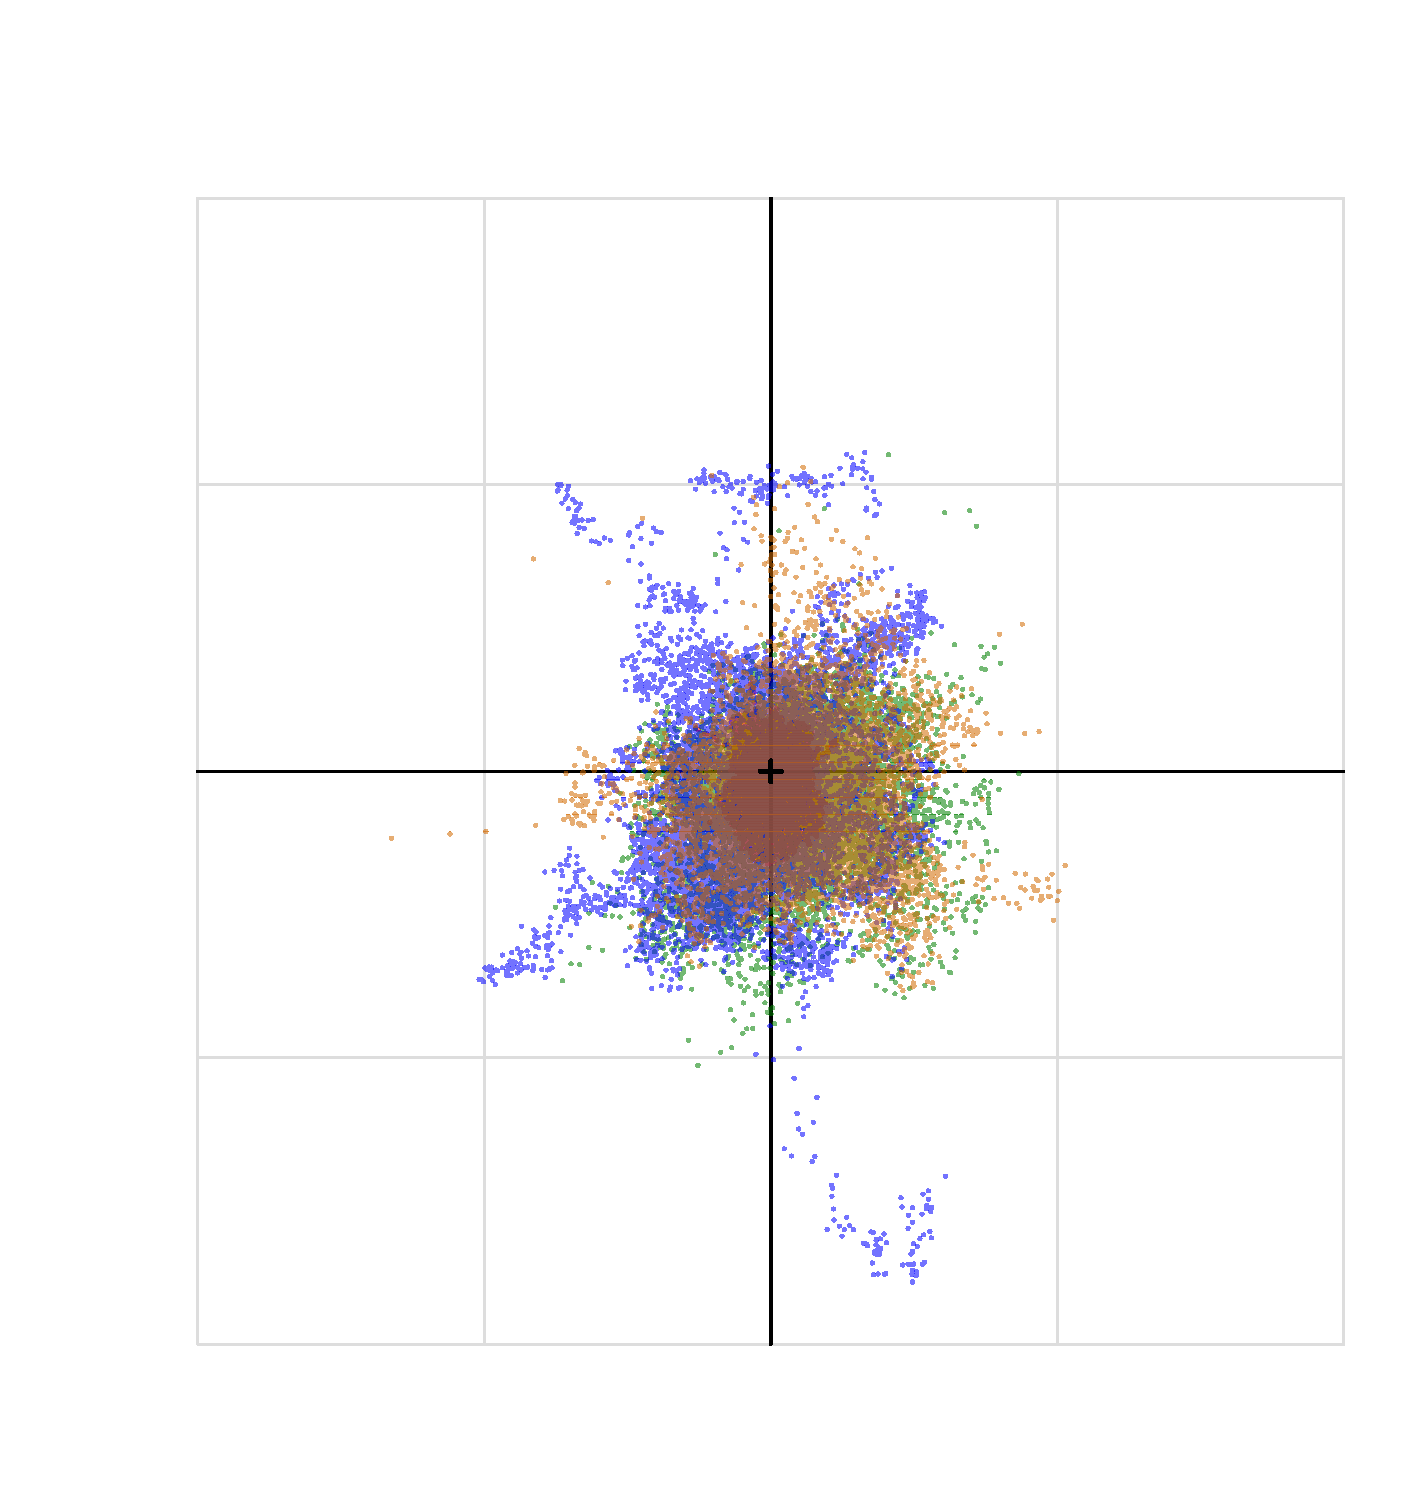
\includegraphics[width=680.0bp,height=715.0bp]{figures/horizontal.pdf}}
\put(95.0,692.0){\makebox(0,0)[lb]{\color{black}\sffamily\fontsize{16}{16}\selectfont Horizontale Abweichungen vom zeitgleichen Sollkreis}}
\put(95.0,50.0){\makebox(0,0)[cb]{\color{black}\sffamily\fontsize{12}{12}\selectfont -0.1}}
\put(232.5,50.0){\makebox(0,0)[cb]{\color{black}\sffamily\fontsize{12}{12}\selectfont -0.05}}
\put(370.0,50.0){\makebox(0,0)[cb]{\color{black}\sffamily\fontsize{12}{12}\selectfont 0}}
\put(507.50000000000006,50.0){\makebox(0,0)[cb]{\color{black}\sffamily\fontsize{12}{12}\selectfont 0.05}}
\put(645.0,50.0){\makebox(0,0)[cb]{\color{black}\sffamily\fontsize{12}{12}\selectfont 0.1}}
\put(87.0,66.0){\makebox(0,0)[rb]{\color{black}\sffamily\fontsize{12}{12}\selectfont -0.1}}
\put(87.0,203.5){\makebox(0,0)[rb]{\color{black}\sffamily\fontsize{12}{12}\selectfont -0.05}}
\put(87.0,341.0){\makebox(0,0)[rb]{\color{black}\sffamily\fontsize{12}{12}\selectfont 0}}
\put(87.0,478.50000000000006){\makebox(0,0)[rb]{\color{black}\sffamily\fontsize{12}{12}\selectfont 0.05}}
\put(87.0,616.0){\makebox(0,0)[rb]{\color{black}\sffamily\fontsize{12}{12}\selectfont 0.1}}
\put(95.0,670.0){\makebox(0,0)[lb]{\color{red}\sffamily\fontsize{12}{12}\selectfont P23M\_0}}
\put(370.0,670.0){\makebox(0,0)[lb]{\color{green}\sffamily\fontsize{12}{12}\selectfont P23M\_1}}
\put(95.0,648.0){\makebox(0,0)[lb]{\color{blue}\sffamily\fontsize{12}{12}\selectfont UM980}}
\put(370.0,648.0){\makebox(0,0)[lb]{\color[HTML]{d26900}\sffamily\fontsize{12}{12}\selectfont LG290P}}
\put(378.0,353.0){\makebox(0,0)[lb]{\color{black}\sffamily\fontsize{12}{12}\selectfont Soll (0,0)}}
\put(370.0,12.0){\makebox(0,0)[cb]{\color{black}\sffamily\fontsize{12}{12}\selectfont Ost-Abweichung [m]}}
\put(19.0,345.0){\rotatebox{90}{\makebox(0,0)[b]{\color{black}\sffamily\fontsize{12}{12}\selectfont Nord-Abweichung [m]}}}
\end{picture}}
\end{figure}
\begin{figure}[p]\centering
\resizebox{0.98\linewidth}{!}{%
\setlength{\unitlength}{1bp}\begin{picture}(680.0,715.0)
\put(0,0){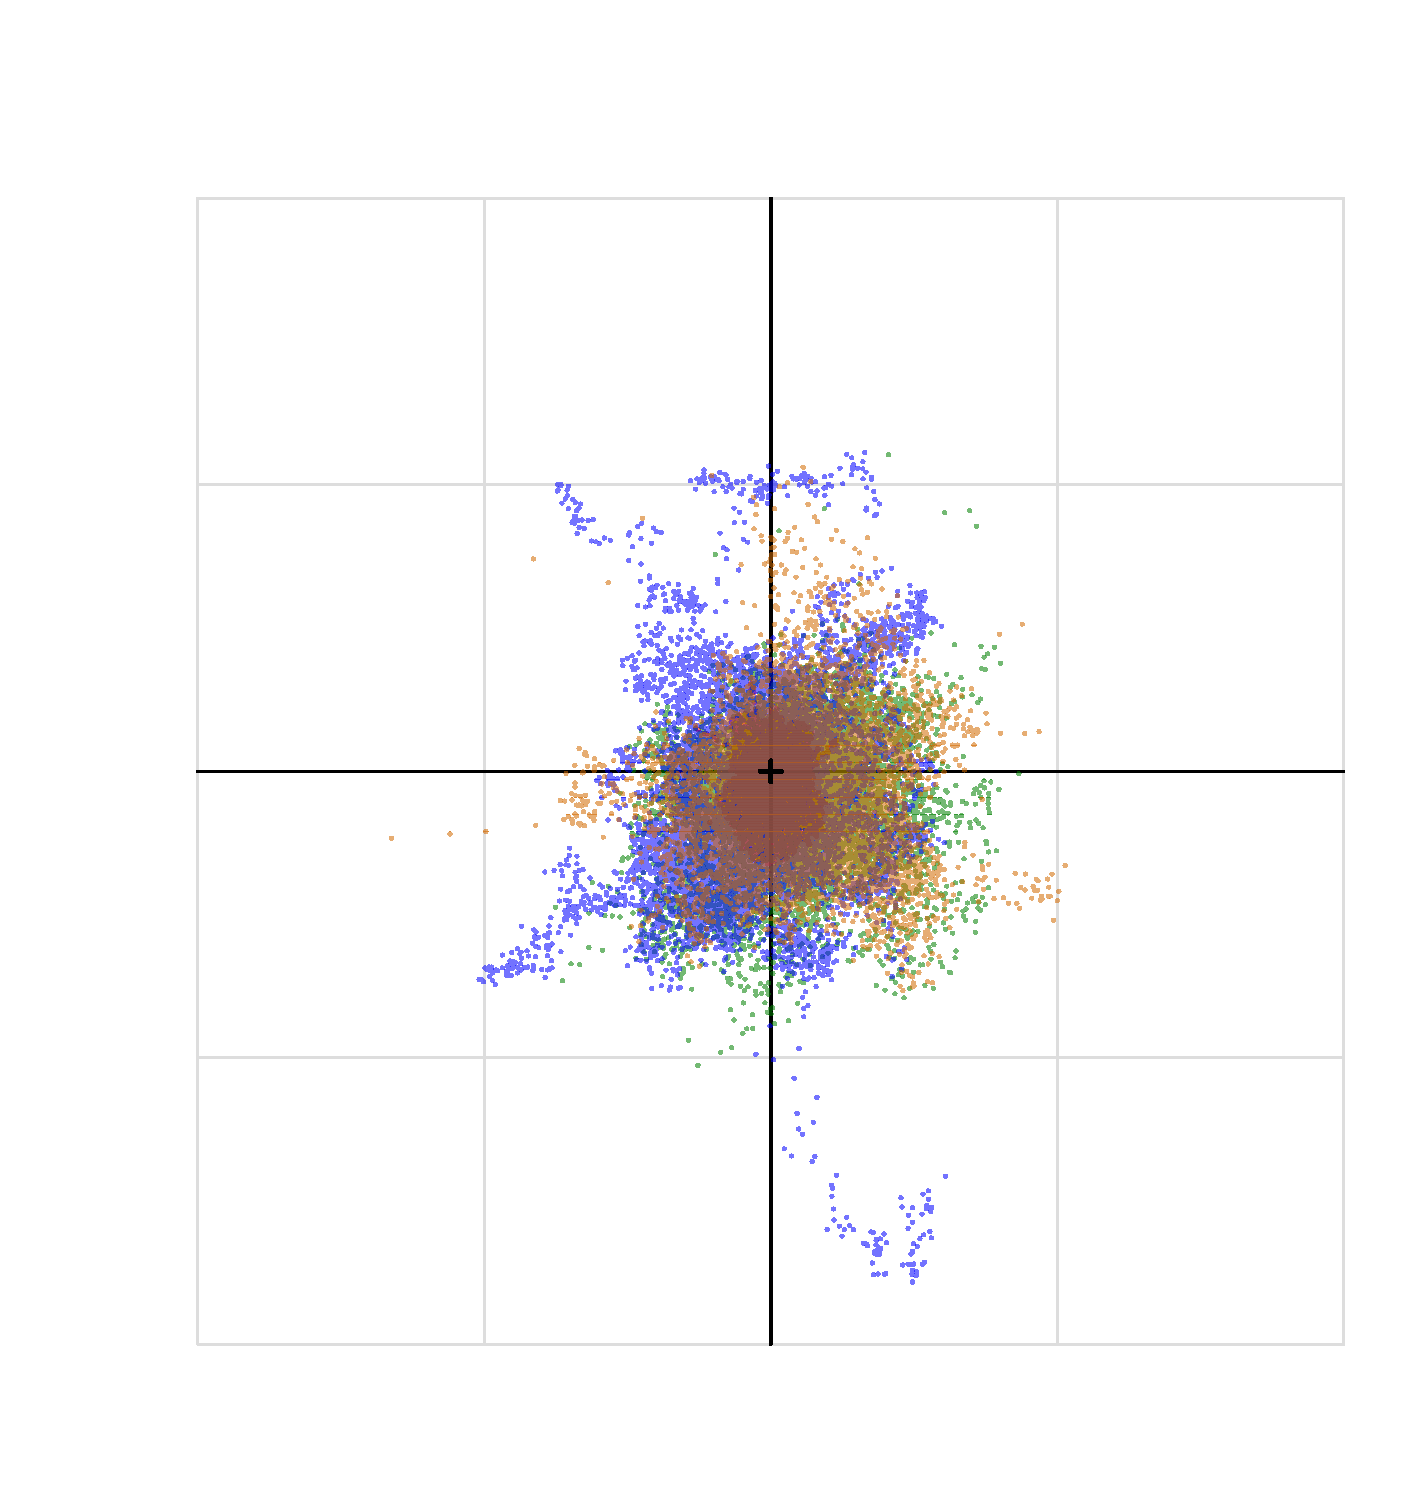
\includegraphics[width=680.0bp,height=715.0bp]{figures/horizontal_detail.pdf}}
\put(95.0,692.0){\makebox(0,0)[lb]{\color{black}\sffamily\fontsize{16}{16}\selectfont Detail ±0,10 m (größere Abweichungen ausgeblendet)}}
\put(95.0,50.0){\makebox(0,0)[cb]{\color{black}\sffamily\fontsize{12}{12}\selectfont -0.1}}
\put(232.5,50.0){\makebox(0,0)[cb]{\color{black}\sffamily\fontsize{12}{12}\selectfont -0.05}}
\put(370.0,50.0){\makebox(0,0)[cb]{\color{black}\sffamily\fontsize{12}{12}\selectfont 0}}
\put(507.50000000000006,50.0){\makebox(0,0)[cb]{\color{black}\sffamily\fontsize{12}{12}\selectfont 0.05}}
\put(645.0,50.0){\makebox(0,0)[cb]{\color{black}\sffamily\fontsize{12}{12}\selectfont 0.1}}
\put(87.0,66.0){\makebox(0,0)[rb]{\color{black}\sffamily\fontsize{12}{12}\selectfont -0.1}}
\put(87.0,203.5){\makebox(0,0)[rb]{\color{black}\sffamily\fontsize{12}{12}\selectfont -0.05}}
\put(87.0,341.0){\makebox(0,0)[rb]{\color{black}\sffamily\fontsize{12}{12}\selectfont 0}}
\put(87.0,478.50000000000006){\makebox(0,0)[rb]{\color{black}\sffamily\fontsize{12}{12}\selectfont 0.05}}
\put(87.0,616.0){\makebox(0,0)[rb]{\color{black}\sffamily\fontsize{12}{12}\selectfont 0.1}}
\put(95.0,670.0){\makebox(0,0)[lb]{\color{red}\sffamily\fontsize{12}{12}\selectfont P23M\_0}}
\put(370.0,670.0){\makebox(0,0)[lb]{\color{green}\sffamily\fontsize{12}{12}\selectfont P23M\_1}}
\put(95.0,648.0){\makebox(0,0)[lb]{\color{blue}\sffamily\fontsize{12}{12}\selectfont UM980}}
\put(370.0,648.0){\makebox(0,0)[lb]{\color[HTML]{d26900}\sffamily\fontsize{12}{12}\selectfont LG290P}}
\put(378.0,353.0){\makebox(0,0)[lb]{\color{black}\sffamily\fontsize{12}{12}\selectfont Soll (0,0)}}
\put(370.0,12.0){\makebox(0,0)[cb]{\color{black}\sffamily\fontsize{12}{12}\selectfont Ost-Abweichung [m]}}
\put(19.0,345.0){\rotatebox{90}{\makebox(0,0)[b]{\color{black}\sffamily\fontsize{12}{12}\selectfont Nord-Abweichung [m]}}}
\end{picture}}
\end{figure}
\begin{figure}[p]\centering
\resizebox{0.98\linewidth}{!}{%
\setlength{\unitlength}{1bp}\begin{picture}(1000.0,430.0)
\put(0,0){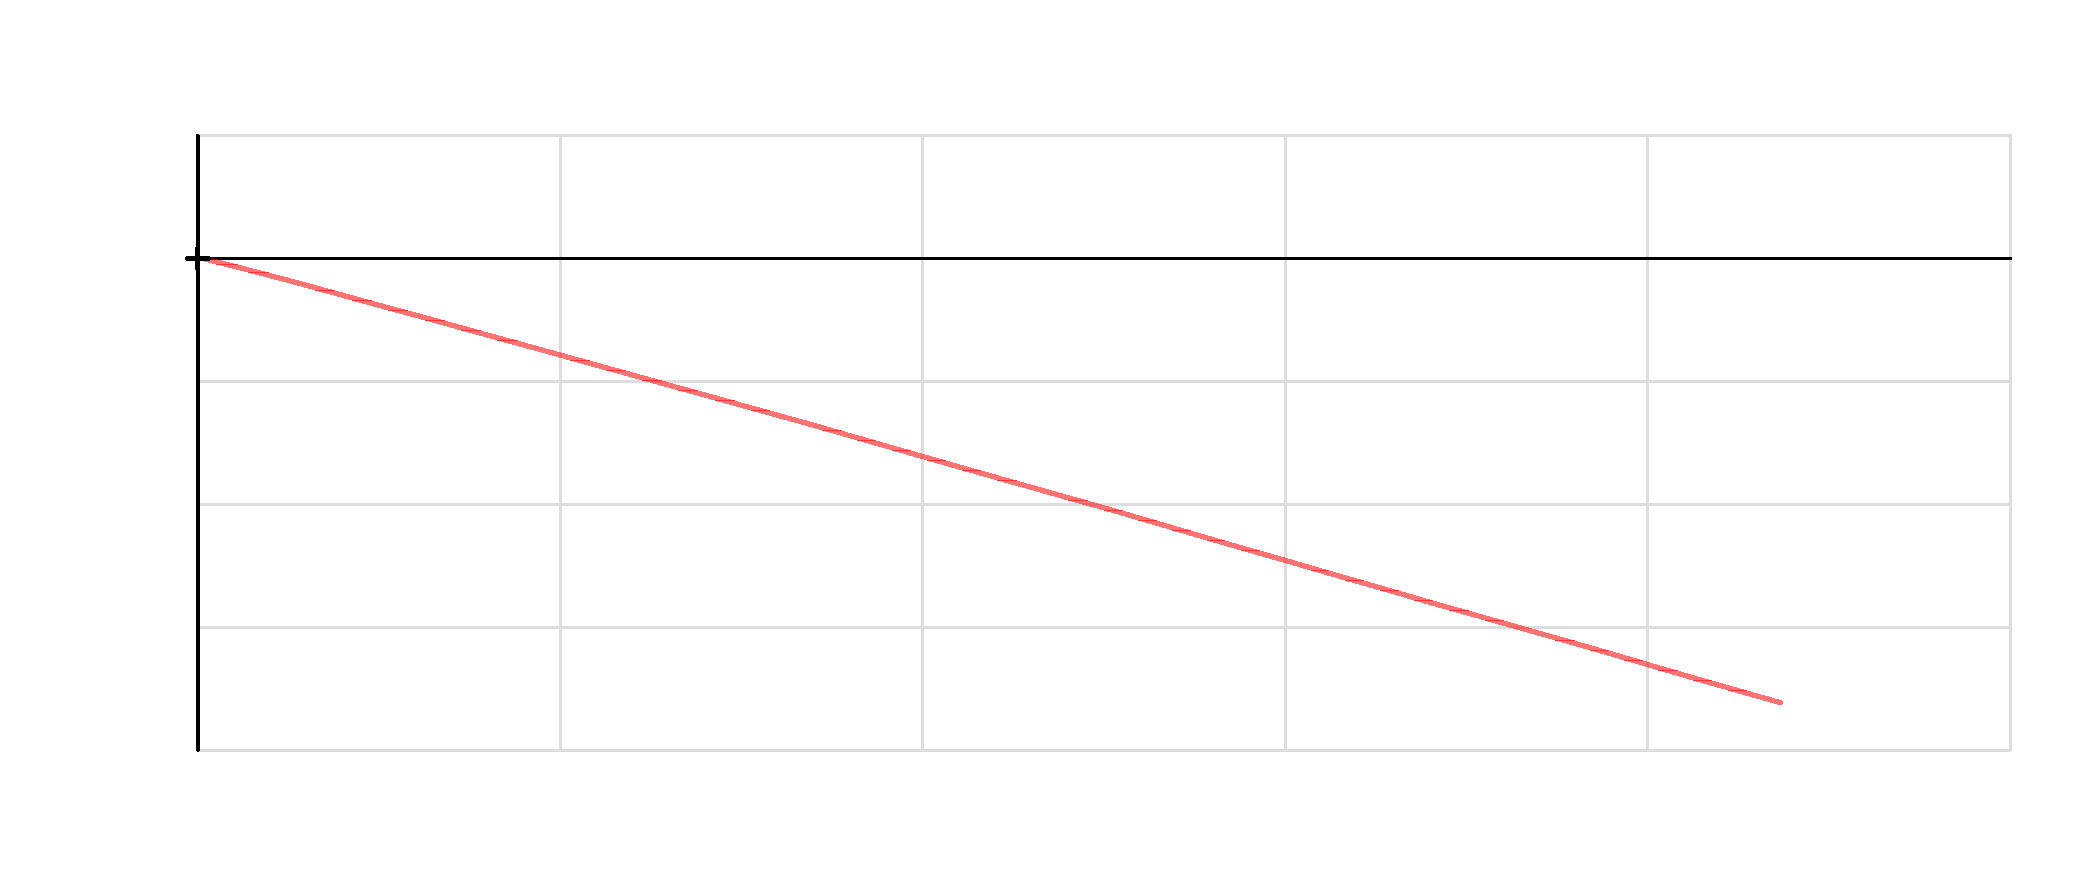
\includegraphics[width=1000.0bp,height=430.0bp]{figures/rotation.pdf}}
\put(95.0,407.0){\makebox(0,0)[lb]{\color{black}\sffamily\fontsize{16}{16}\selectfont Umdrehungen: positiv von Ost nach Nord}}
\put(95.0,50.0){\makebox(0,0)[cb]{\color{black}\sffamily\fontsize{12}{12}\selectfont 0}}
\put(269.0,50.0){\makebox(0,0)[cb]{\color{black}\sffamily\fontsize{12}{12}\selectfont 50}}
\put(443.0,50.0){\makebox(0,0)[cb]{\color{black}\sffamily\fontsize{12}{12}\selectfont 100}}
\put(617.0,50.0){\makebox(0,0)[cb]{\color{black}\sffamily\fontsize{12}{12}\selectfont 150}}
\put(791.0,50.0){\makebox(0,0)[cb]{\color{black}\sffamily\fontsize{12}{12}\selectfont 200}}
\put(965.0,50.0){\makebox(0,0)[cb]{\color{black}\sffamily\fontsize{12}{12}\selectfont 250}}
\put(87.0,66.0){\makebox(0,0)[rb]{\color{black}\sffamily\fontsize{12}{12}\selectfont -80}}
\put(87.0,125.0){\makebox(0,0)[rb]{\color{black}\sffamily\fontsize{12}{12}\selectfont -60}}
\put(87.0,184.0){\makebox(0,0)[rb]{\color{black}\sffamily\fontsize{12}{12}\selectfont -40}}
\put(87.0,243.0){\makebox(0,0)[rb]{\color{black}\sffamily\fontsize{12}{12}\selectfont -20}}
\put(87.0,302.0){\makebox(0,0)[rb]{\color{black}\sffamily\fontsize{12}{12}\selectfont 0}}
\put(87.0,361.0){\makebox(0,0)[rb]{\color{black}\sffamily\fontsize{12}{12}\selectfont 20}}
\put(95.0,385.0){\makebox(0,0)[lb]{\color{red}\sffamily\fontsize{12}{12}\selectfont P23M\_0}}
\put(103.0,314.0){\makebox(0,0)[lb]{\color{black}\sffamily\fontsize{12}{12}\selectfont (0,0)}}
\put(530.0,12.0){\makebox(0,0)[cb]{\color{black}\sffamily\fontsize{12}{12}\selectfont Zeit seit gemeinsamem Beginn [min]}}
\put(19.0,217.5){\rotatebox{90}{\makebox(0,0)[b]{\color{black}\sffamily\fontsize{12}{12}\selectfont Anzahl der Vollkreise seit erstem Referenzpunkt}}}
\end{picture}}
\end{figure}
\begin{figure}[p]\centering
\resizebox{0.98\linewidth}{!}{%
\setlength{\unitlength}{1bp}\begin{picture}(1000.0,435.0)
\put(0,0){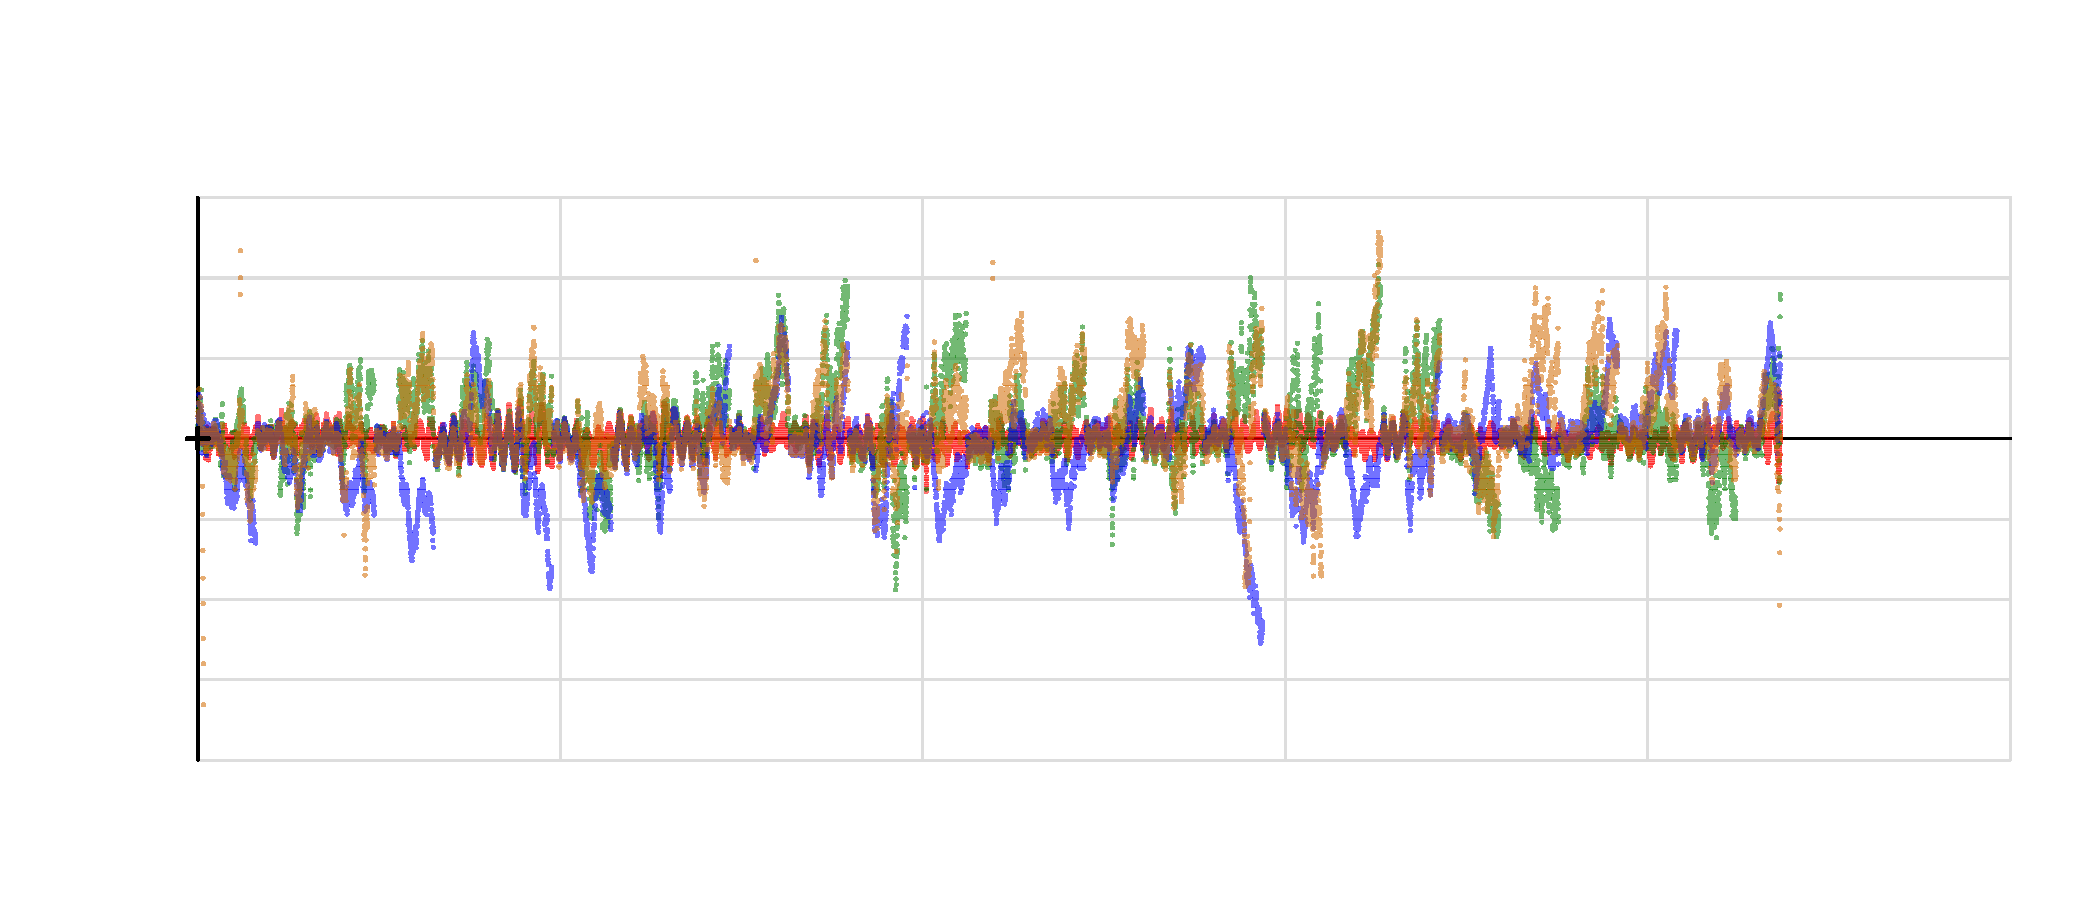
\includegraphics[width=1000.0bp,height=435.0bp]{figures/east_time.pdf}}
\put(95.0,412.0){\makebox(0,0)[lb]{\color{black}\sffamily\fontsize{16}{16}\selectfont Ost-Abweichung über der Zeit}}
\put(95.0,50.0){\makebox(0,0)[cb]{\color{black}\sffamily\fontsize{12}{12}\selectfont 0}}
\put(269.0,50.0){\makebox(0,0)[cb]{\color{black}\sffamily\fontsize{12}{12}\selectfont 50}}
\put(443.0,50.0){\makebox(0,0)[cb]{\color{black}\sffamily\fontsize{12}{12}\selectfont 100}}
\put(617.0,50.0){\makebox(0,0)[cb]{\color{black}\sffamily\fontsize{12}{12}\selectfont 150}}
\put(791.0,50.0){\makebox(0,0)[cb]{\color{black}\sffamily\fontsize{12}{12}\selectfont 200}}
\put(965.0,50.0){\makebox(0,0)[cb]{\color{black}\sffamily\fontsize{12}{12}\selectfont 250}}
\put(87.0,66.0){\makebox(0,0)[rb]{\color{black}\sffamily\fontsize{12}{12}\selectfont -0.08}}
\put(87.0,104.57142857142856){\makebox(0,0)[rb]{\color{black}\sffamily\fontsize{12}{12}\selectfont -0.06}}
\put(87.0,143.1428571428571){\makebox(0,0)[rb]{\color{black}\sffamily\fontsize{12}{12}\selectfont -0.04}}
\put(87.0,181.7142857142857){\makebox(0,0)[rb]{\color{black}\sffamily\fontsize{12}{12}\selectfont -0.02}}
\put(87.0,220.28571428571428){\makebox(0,0)[rb]{\color{black}\sffamily\fontsize{12}{12}\selectfont 0}}
\put(87.0,258.8571428571429){\makebox(0,0)[rb]{\color{black}\sffamily\fontsize{12}{12}\selectfont 0.02}}
\put(87.0,297.4285714285714){\makebox(0,0)[rb]{\color{black}\sffamily\fontsize{12}{12}\selectfont 0.04}}
\put(87.0,336.0){\makebox(0,0)[rb]{\color{black}\sffamily\fontsize{12}{12}\selectfont 0.06}}
\put(95.0,390.0){\makebox(0,0)[lb]{\color{red}\sffamily\fontsize{12}{12}\selectfont P23M\_0}}
\put(530.0,390.0){\makebox(0,0)[lb]{\color{green}\sffamily\fontsize{12}{12}\selectfont P23M\_1}}
\put(95.0,368.0){\makebox(0,0)[lb]{\color{blue}\sffamily\fontsize{12}{12}\selectfont UM980}}
\put(530.0,368.0){\makebox(0,0)[lb]{\color[HTML]{d26900}\sffamily\fontsize{12}{12}\selectfont LG290P}}
\put(103.0,232.28571428571428){\makebox(0,0)[lb]{\color{black}\sffamily\fontsize{12}{12}\selectfont (0,0)}}
\put(530.0,12.0){\makebox(0,0)[cb]{\color{black}\sffamily\fontsize{12}{12}\selectfont Zeit seit gemeinsamem Beginn [min]}}
\put(19.0,205.0){\rotatebox{90}{\makebox(0,0)[b]{\color{black}\sffamily\fontsize{12}{12}\selectfont Ost-Abweichung [m]}}}
\end{picture}}
\end{figure}
\begin{figure}[p]\centering
\resizebox{0.98\linewidth}{!}{%
\setlength{\unitlength}{1bp}\begin{picture}(1000.0,435.0)
\put(0,0){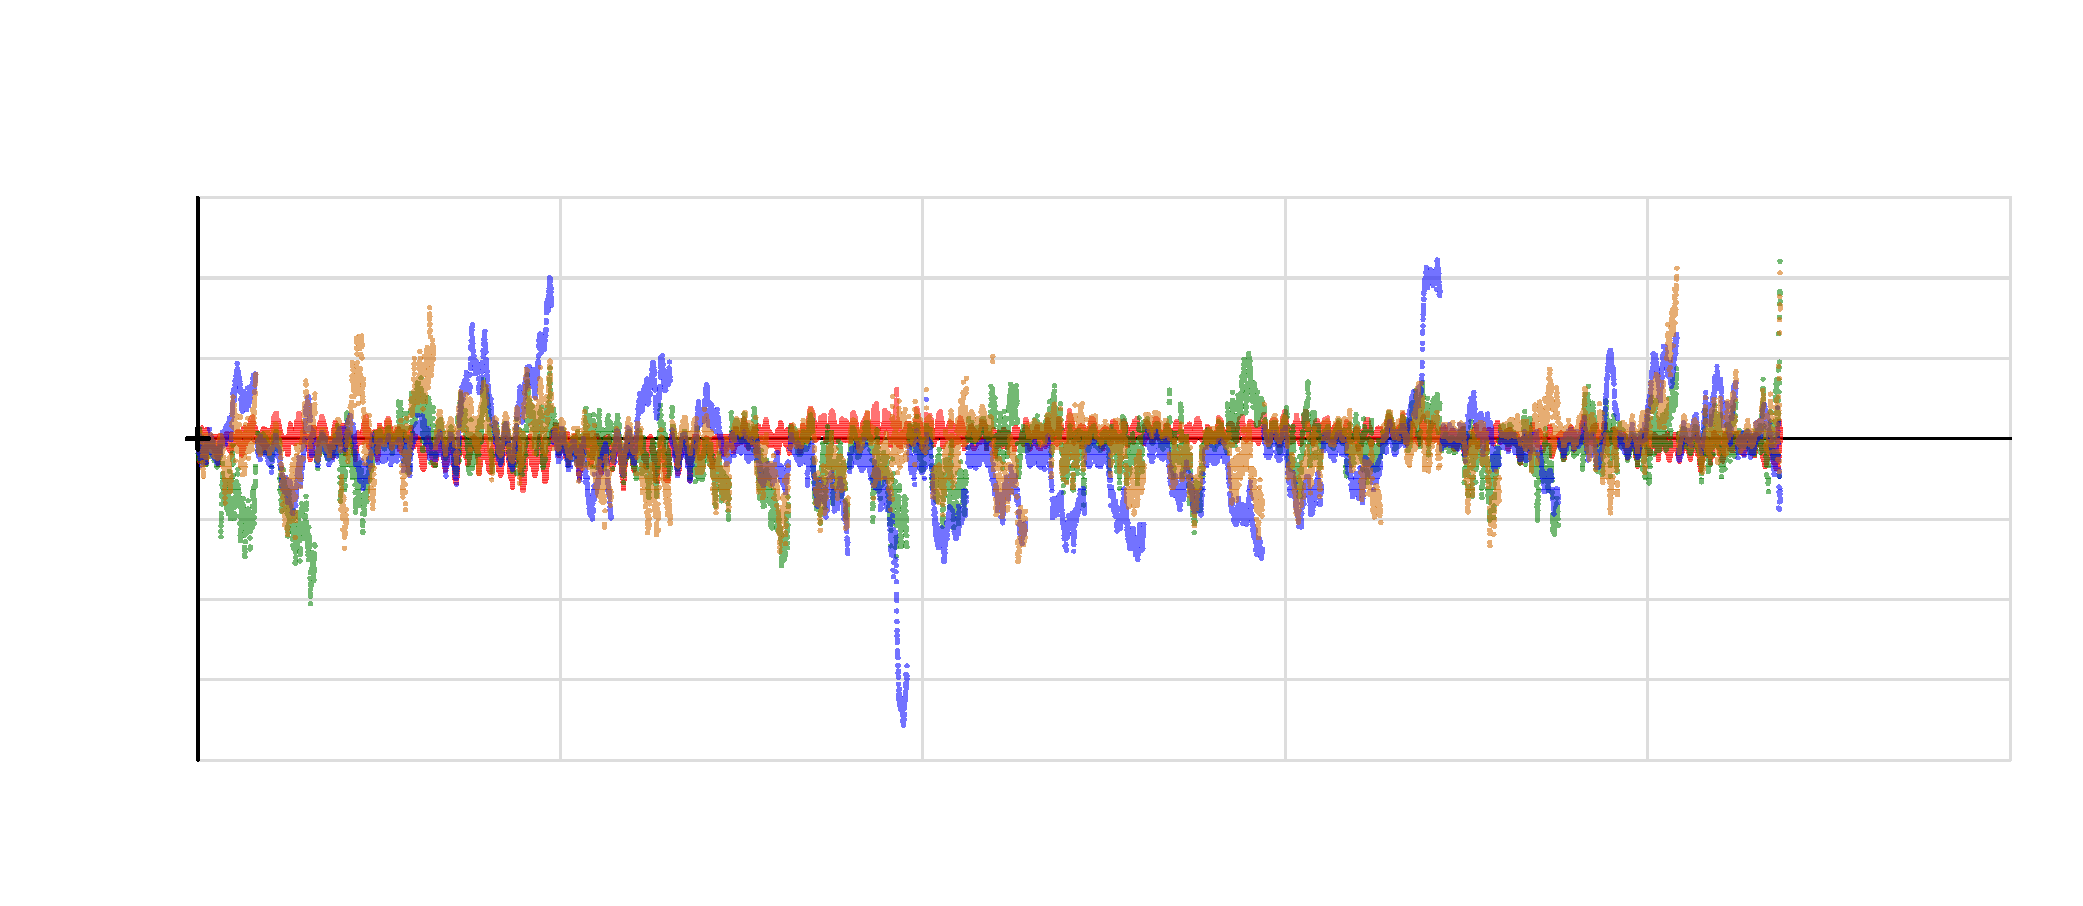
\includegraphics[width=1000.0bp,height=435.0bp]{figures/north_time.pdf}}
\put(95.0,412.0){\makebox(0,0)[lb]{\color{black}\sffamily\fontsize{16}{16}\selectfont Nord-Abweichung über der Zeit}}
\put(95.0,50.0){\makebox(0,0)[cb]{\color{black}\sffamily\fontsize{12}{12}\selectfont 0}}
\put(269.0,50.0){\makebox(0,0)[cb]{\color{black}\sffamily\fontsize{12}{12}\selectfont 50}}
\put(443.0,50.0){\makebox(0,0)[cb]{\color{black}\sffamily\fontsize{12}{12}\selectfont 100}}
\put(617.0,50.0){\makebox(0,0)[cb]{\color{black}\sffamily\fontsize{12}{12}\selectfont 150}}
\put(791.0,50.0){\makebox(0,0)[cb]{\color{black}\sffamily\fontsize{12}{12}\selectfont 200}}
\put(965.0,50.0){\makebox(0,0)[cb]{\color{black}\sffamily\fontsize{12}{12}\selectfont 250}}
\put(87.0,66.0){\makebox(0,0)[rb]{\color{black}\sffamily\fontsize{12}{12}\selectfont -0.1}}
\put(87.0,104.57142857142856){\makebox(0,0)[rb]{\color{black}\sffamily\fontsize{12}{12}\selectfont -0.075}}
\put(87.0,143.1428571428571){\makebox(0,0)[rb]{\color{black}\sffamily\fontsize{12}{12}\selectfont -0.05}}
\put(87.0,181.71428571428572){\makebox(0,0)[rb]{\color{black}\sffamily\fontsize{12}{12}\selectfont -0.025}}
\put(87.0,220.28571428571428){\makebox(0,0)[rb]{\color{black}\sffamily\fontsize{12}{12}\selectfont 0}}
\put(87.0,258.85714285714283){\makebox(0,0)[rb]{\color{black}\sffamily\fontsize{12}{12}\selectfont 0.025}}
\put(87.0,297.42857142857144){\makebox(0,0)[rb]{\color{black}\sffamily\fontsize{12}{12}\selectfont 0.05}}
\put(87.0,336.0){\makebox(0,0)[rb]{\color{black}\sffamily\fontsize{12}{12}\selectfont 0.075}}
\put(95.0,390.0){\makebox(0,0)[lb]{\color{red}\sffamily\fontsize{12}{12}\selectfont P23M\_0}}
\put(530.0,390.0){\makebox(0,0)[lb]{\color{green}\sffamily\fontsize{12}{12}\selectfont P23M\_1}}
\put(95.0,368.0){\makebox(0,0)[lb]{\color{blue}\sffamily\fontsize{12}{12}\selectfont UM980}}
\put(530.0,368.0){\makebox(0,0)[lb]{\color[HTML]{d26900}\sffamily\fontsize{12}{12}\selectfont LG290P}}
\put(103.0,232.28571428571428){\makebox(0,0)[lb]{\color{black}\sffamily\fontsize{12}{12}\selectfont (0,0)}}
\put(530.0,12.0){\makebox(0,0)[cb]{\color{black}\sffamily\fontsize{12}{12}\selectfont Zeit seit gemeinsamem Beginn [min]}}
\put(19.0,205.0){\rotatebox{90}{\makebox(0,0)[b]{\color{black}\sffamily\fontsize{12}{12}\selectfont Nord-Abweichung [m]}}}
\end{picture}}
\end{figure}
\begin{figure}[p]\centering
\resizebox{0.98\linewidth}{!}{%
\setlength{\unitlength}{1bp}\begin{picture}(1000.0,435.0)
\put(0,0){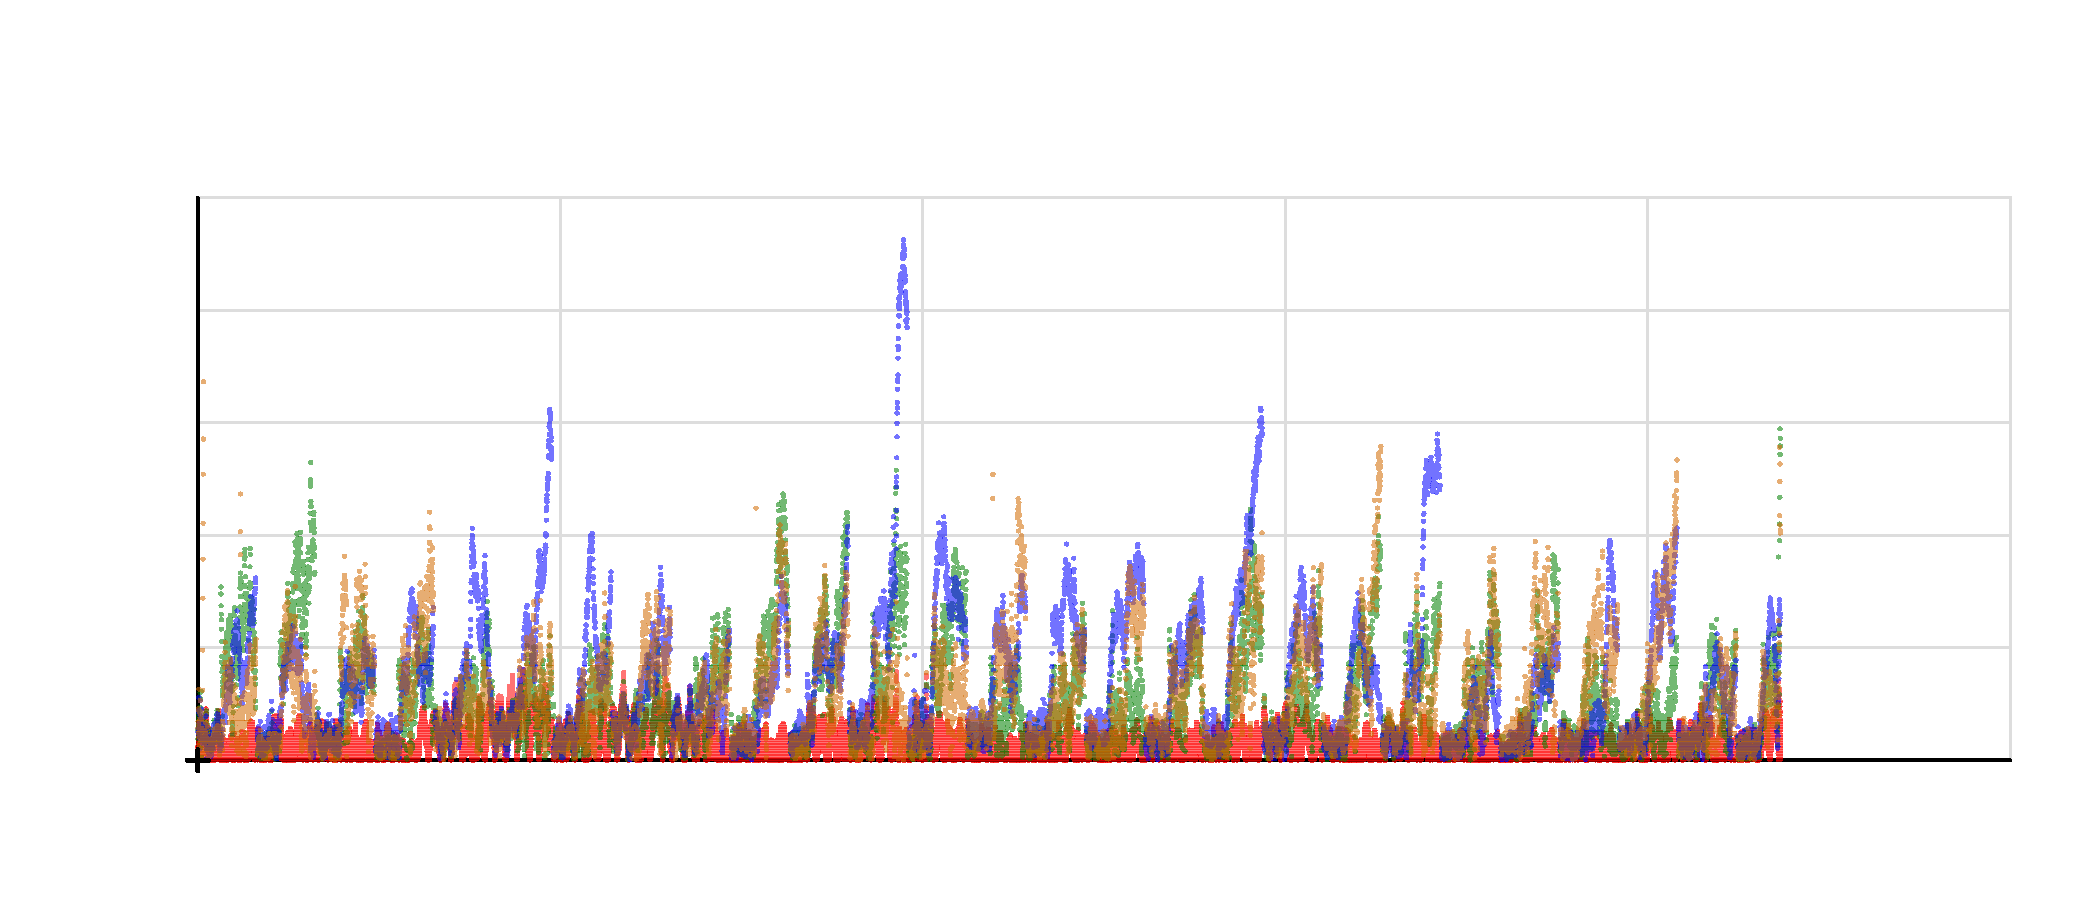
\includegraphics[width=1000.0bp,height=435.0bp]{figures/horizontal_time.pdf}}
\put(95.0,412.0){\makebox(0,0)[lb]{\color{black}\sffamily\fontsize{16}{16}\selectfont Horizontal-Abweichung über der Zeit}}
\put(95.0,50.0){\makebox(0,0)[cb]{\color{black}\sffamily\fontsize{12}{12}\selectfont 0}}
\put(269.0,50.0){\makebox(0,0)[cb]{\color{black}\sffamily\fontsize{12}{12}\selectfont 50}}
\put(443.0,50.0){\makebox(0,0)[cb]{\color{black}\sffamily\fontsize{12}{12}\selectfont 100}}
\put(617.0,50.0){\makebox(0,0)[cb]{\color{black}\sffamily\fontsize{12}{12}\selectfont 150}}
\put(791.0,50.0){\makebox(0,0)[cb]{\color{black}\sffamily\fontsize{12}{12}\selectfont 200}}
\put(965.0,50.0){\makebox(0,0)[cb]{\color{black}\sffamily\fontsize{12}{12}\selectfont 250}}
\put(87.0,66.0){\makebox(0,0)[rb]{\color{black}\sffamily\fontsize{12}{12}\selectfont 0}}
\put(87.0,120.0){\makebox(0,0)[rb]{\color{black}\sffamily\fontsize{12}{12}\selectfont 0.02}}
\put(87.0,174.0){\makebox(0,0)[rb]{\color{black}\sffamily\fontsize{12}{12}\selectfont 0.04}}
\put(87.0,228.0){\makebox(0,0)[rb]{\color{black}\sffamily\fontsize{12}{12}\selectfont 0.06}}
\put(87.0,282.0){\makebox(0,0)[rb]{\color{black}\sffamily\fontsize{12}{12}\selectfont 0.08}}
\put(87.0,336.0){\makebox(0,0)[rb]{\color{black}\sffamily\fontsize{12}{12}\selectfont 0.1}}
\put(95.0,390.0){\makebox(0,0)[lb]{\color{red}\sffamily\fontsize{12}{12}\selectfont P23M\_0}}
\put(530.0,390.0){\makebox(0,0)[lb]{\color{green}\sffamily\fontsize{12}{12}\selectfont P23M\_1}}
\put(95.0,368.0){\makebox(0,0)[lb]{\color{blue}\sffamily\fontsize{12}{12}\selectfont UM980}}
\put(530.0,368.0){\makebox(0,0)[lb]{\color[HTML]{d26900}\sffamily\fontsize{12}{12}\selectfont LG290P}}
\put(103.0,78.0){\makebox(0,0)[lb]{\color{black}\sffamily\fontsize{12}{12}\selectfont (0,0)}}
\put(530.0,12.0){\makebox(0,0)[cb]{\color{black}\sffamily\fontsize{12}{12}\selectfont Zeit seit gemeinsamem Beginn [min]}}
\put(19.0,205.0){\rotatebox{90}{\makebox(0,0)[b]{\color{black}\sffamily\fontsize{12}{12}\selectfont Horizontal-Abweichung [m]}}}
\end{picture}}
\end{figure}
\begin{figure}[p]\centering
\resizebox{0.98\linewidth}{!}{%
\setlength{\unitlength}{1bp}\begin{picture}(1000.0,435.0)
\put(0,0){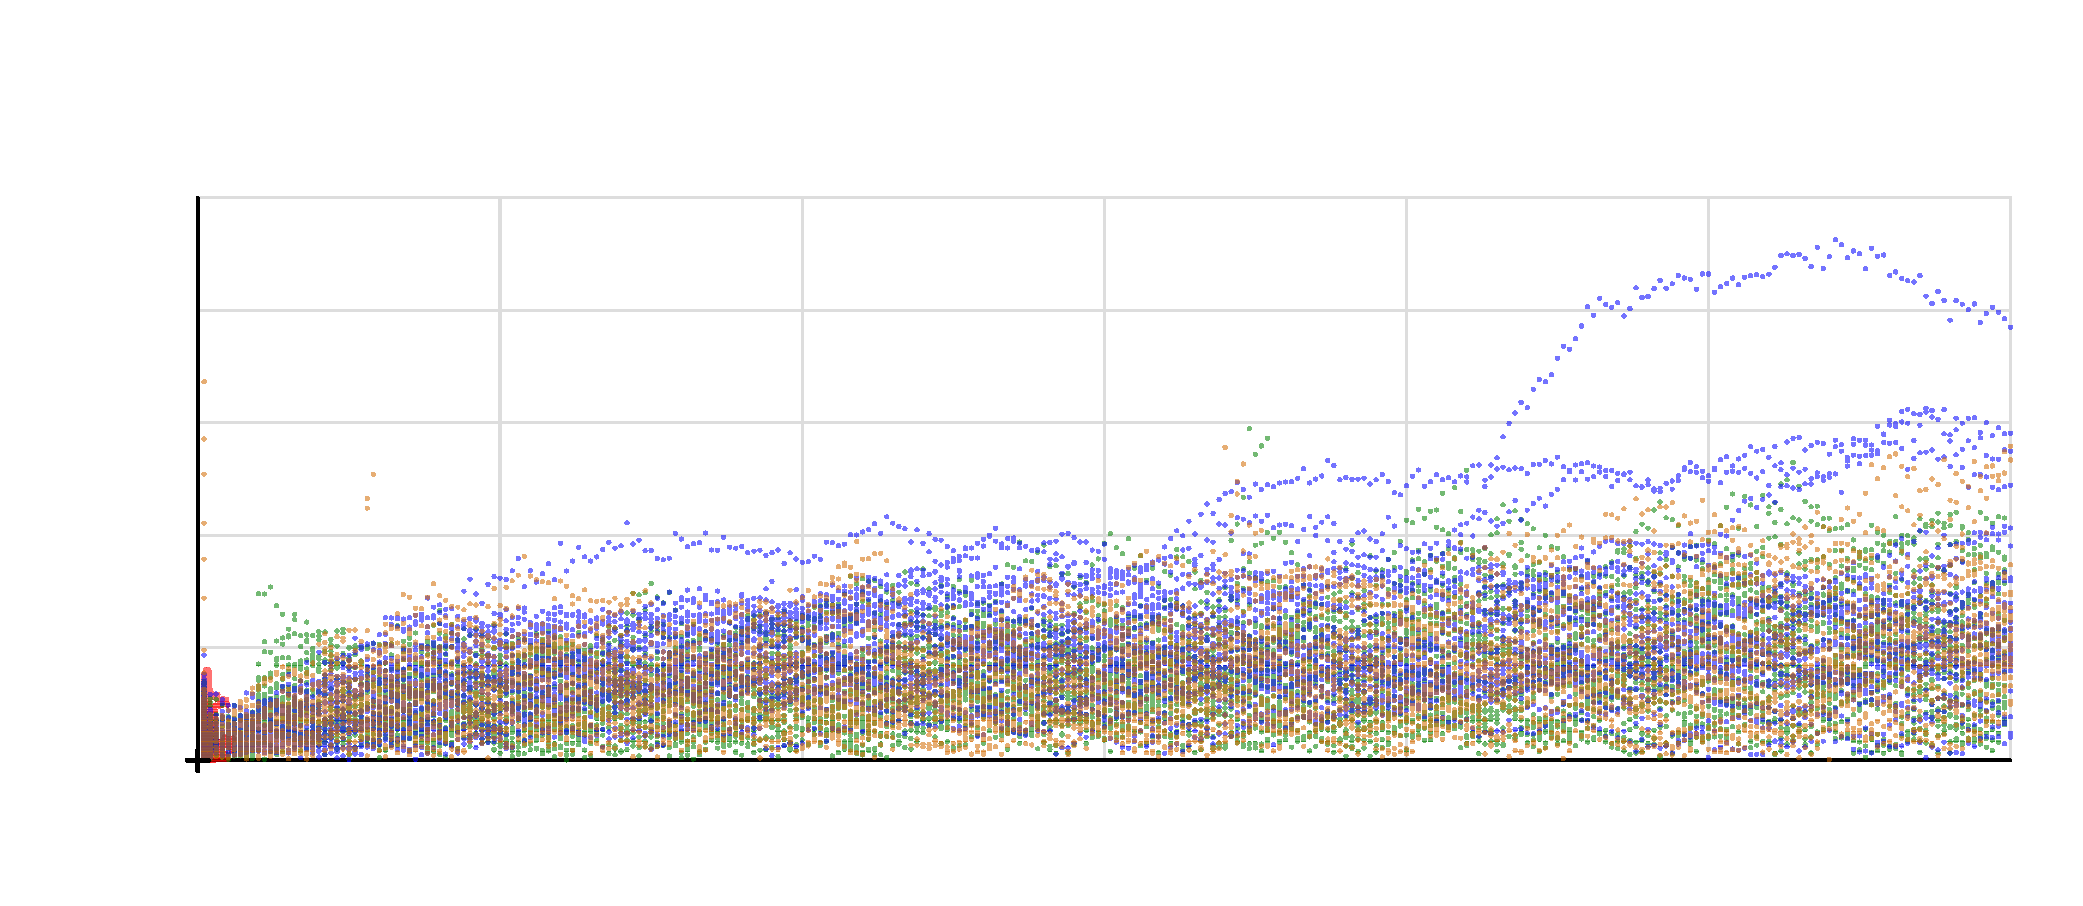
\includegraphics[width=1000.0bp,height=435.0bp]{figures/horizontal_dage_scatter.pdf}}
\put(95.0,412.0){\makebox(0,0)[lb]{\color{black}\sffamily\fontsize{16}{16}\selectfont Horizontaler Fehler über dAge: alle RTK-fixed-Einzelwerte}}
\put(95.0,50.0){\makebox(0,0)[cb]{\color{black}\sffamily\fontsize{12}{12}\selectfont 0}}
\put(240.0,50.0){\makebox(0,0)[cb]{\color{black}\sffamily\fontsize{12}{12}\selectfont 50}}
\put(385.0,50.0){\makebox(0,0)[cb]{\color{black}\sffamily\fontsize{12}{12}\selectfont 100}}
\put(530.0,50.0){\makebox(0,0)[cb]{\color{black}\sffamily\fontsize{12}{12}\selectfont 150}}
\put(675.0,50.0){\makebox(0,0)[cb]{\color{black}\sffamily\fontsize{12}{12}\selectfont 200}}
\put(820.0,50.0){\makebox(0,0)[cb]{\color{black}\sffamily\fontsize{12}{12}\selectfont 250}}
\put(965.0,50.0){\makebox(0,0)[cb]{\color{black}\sffamily\fontsize{12}{12}\selectfont 300}}
\put(87.0,66.0){\makebox(0,0)[rb]{\color{black}\sffamily\fontsize{12}{12}\selectfont 0}}
\put(87.0,120.0){\makebox(0,0)[rb]{\color{black}\sffamily\fontsize{12}{12}\selectfont 20}}
\put(87.0,174.0){\makebox(0,0)[rb]{\color{black}\sffamily\fontsize{12}{12}\selectfont 40}}
\put(87.0,228.0){\makebox(0,0)[rb]{\color{black}\sffamily\fontsize{12}{12}\selectfont 60}}
\put(87.0,282.0){\makebox(0,0)[rb]{\color{black}\sffamily\fontsize{12}{12}\selectfont 80}}
\put(87.0,336.0){\makebox(0,0)[rb]{\color{black}\sffamily\fontsize{12}{12}\selectfont 100}}
\put(95.0,390.0){\makebox(0,0)[lb]{\color{red}\sffamily\fontsize{12}{12}\selectfont P23M\_0}}
\put(530.0,390.0){\makebox(0,0)[lb]{\color{green}\sffamily\fontsize{12}{12}\selectfont P23M\_1}}
\put(95.0,368.0){\makebox(0,0)[lb]{\color{blue}\sffamily\fontsize{12}{12}\selectfont UM980}}
\put(530.0,368.0){\makebox(0,0)[lb]{\color[HTML]{d26900}\sffamily\fontsize{12}{12}\selectfont LG290P}}
\put(103.0,78.0){\makebox(0,0)[lb]{\color{black}\sffamily\fontsize{12}{12}\selectfont (0,0)}}
\put(530.0,12.0){\makebox(0,0)[cb]{\color{black}\sffamily\fontsize{12}{12}\selectfont Korrekturdatenalter dAge [s]}}
\put(19.0,205.0){\rotatebox{90}{\makebox(0,0)[b]{\color{black}\sffamily\fontsize{12}{12}\selectfont Horizontaler Fehler [mm]}}}
\end{picture}}
\end{figure}
\begin{figure}[p]\centering
\resizebox{0.98\linewidth}{!}{%
\setlength{\unitlength}{1bp}\begin{picture}(1000.0,479.0)
\put(0,0){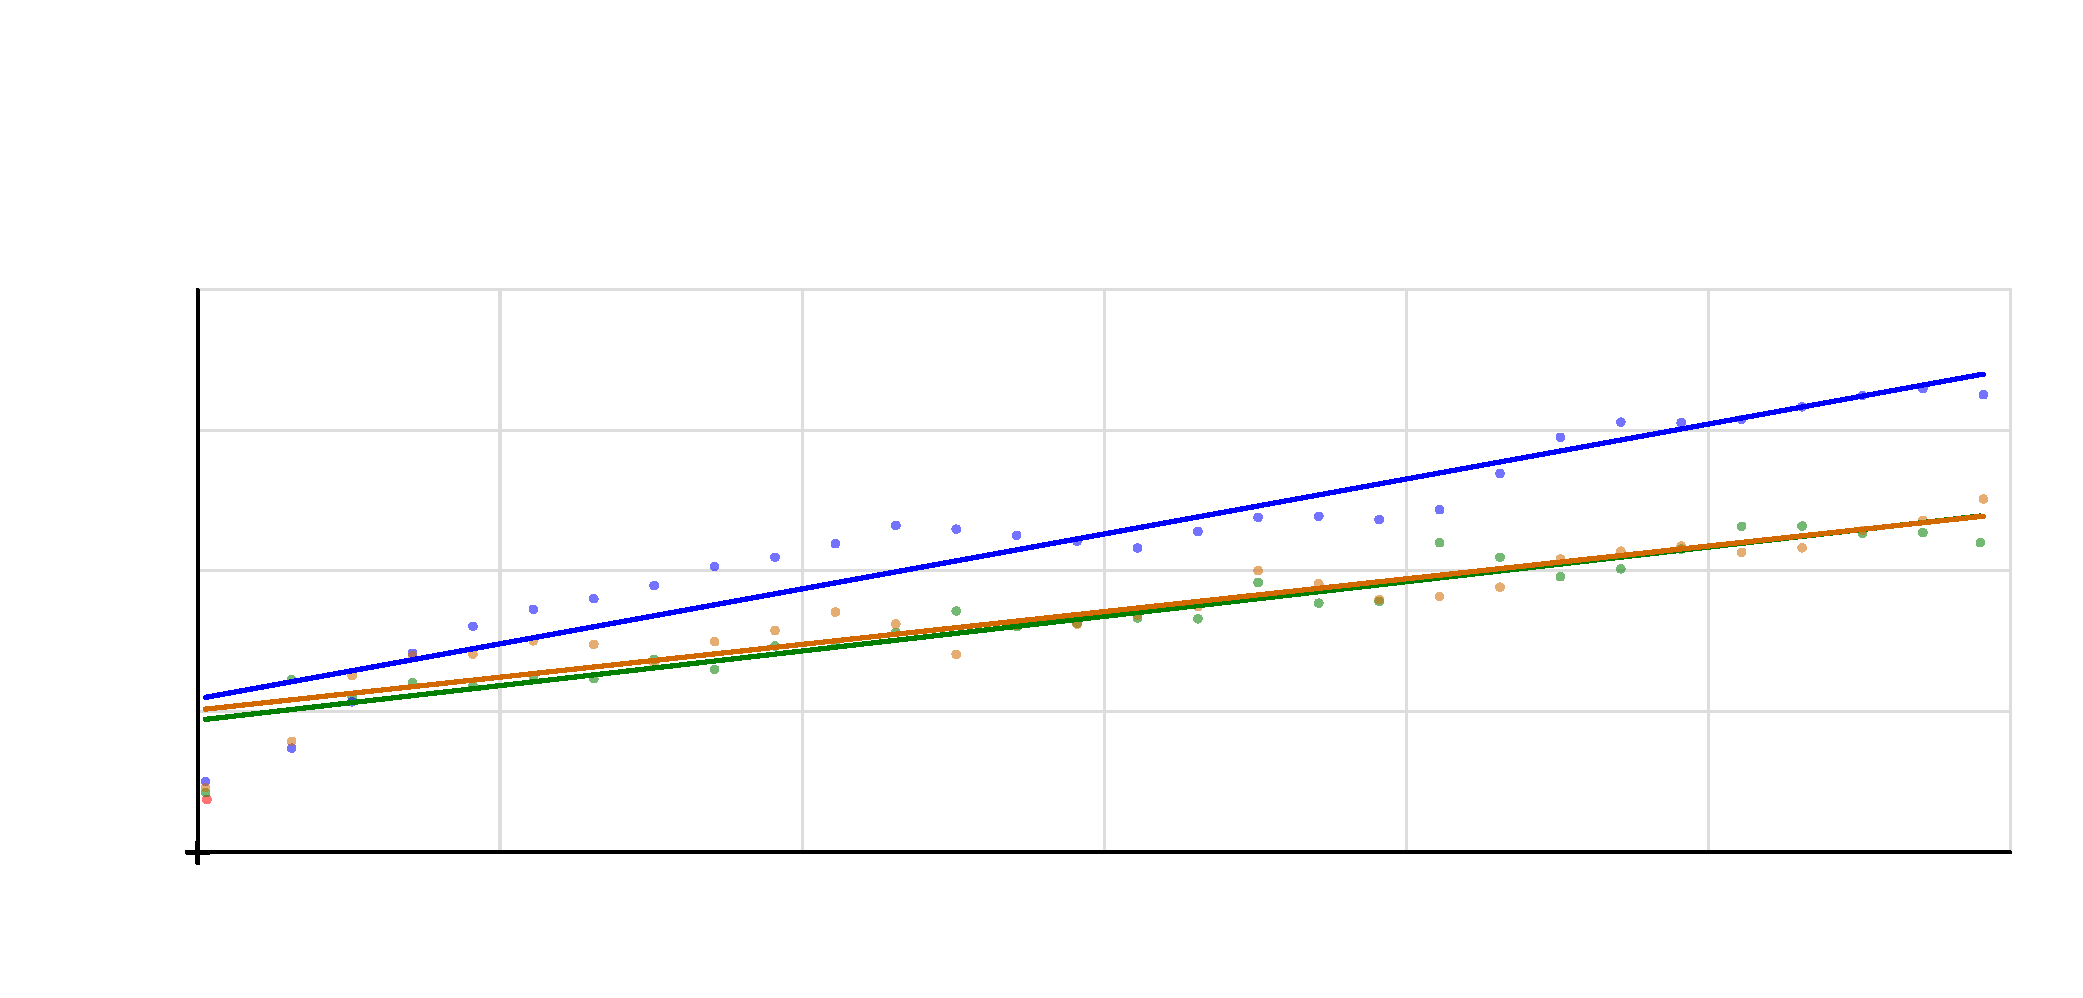
\includegraphics[width=1000.0bp,height=479.0bp]{figures/horizontal_dage.pdf}}
\put(95.0,456.0){\makebox(0,0)[lb]{\color{black}\sffamily\fontsize{16}{16}\selectfont HRMS über dAge: 10-s-Intervalle und linearer Fit}}
\put(95.0,50.0){\makebox(0,0)[cb]{\color{black}\sffamily\fontsize{12}{12}\selectfont 0}}
\put(240.0,50.0){\makebox(0,0)[cb]{\color{black}\sffamily\fontsize{12}{12}\selectfont 50}}
\put(385.0,50.0){\makebox(0,0)[cb]{\color{black}\sffamily\fontsize{12}{12}\selectfont 100}}
\put(530.0,50.0){\makebox(0,0)[cb]{\color{black}\sffamily\fontsize{12}{12}\selectfont 150}}
\put(675.0,50.0){\makebox(0,0)[cb]{\color{black}\sffamily\fontsize{12}{12}\selectfont 200}}
\put(820.0,50.0){\makebox(0,0)[cb]{\color{black}\sffamily\fontsize{12}{12}\selectfont 250}}
\put(965.0,50.0){\makebox(0,0)[cb]{\color{black}\sffamily\fontsize{12}{12}\selectfont 300}}
\put(87.0,66.0){\makebox(0,0)[rb]{\color{black}\sffamily\fontsize{12}{12}\selectfont 0}}
\put(87.0,133.5){\makebox(0,0)[rb]{\color{black}\sffamily\fontsize{12}{12}\selectfont 10}}
\put(87.0,201.0){\makebox(0,0)[rb]{\color{black}\sffamily\fontsize{12}{12}\selectfont 20}}
\put(87.0,268.5){\makebox(0,0)[rb]{\color{black}\sffamily\fontsize{12}{12}\selectfont 30}}
\put(87.0,336.0){\makebox(0,0)[rb]{\color{black}\sffamily\fontsize{12}{12}\selectfont 40}}
\put(95.0,434.0){\makebox(0,0)[lb]{\color{red}\sffamily\fontsize{12}{12}\selectfont P23M\_0}}
\put(530.0,434.0){\makebox(0,0)[lb]{\color{green}\sffamily\fontsize{12}{12}\selectfont P23M\_1}}
\put(95.0,412.0){\makebox(0,0)[lb]{\color{blue}\sffamily\fontsize{12}{12}\selectfont UM980}}
\put(530.0,412.0){\makebox(0,0)[lb]{\color[HTML]{d26900}\sffamily\fontsize{12}{12}\selectfont LG290P}}
\put(95.0,390.0){\makebox(0,0)[lb]{\color{green}\sffamily\fontsize{12}{12}\selectfont P23M\_1: +0.0492 mm/\allowbreak{}s}}
\put(530.0,390.0){\makebox(0,0)[lb]{\color{blue}\sffamily\fontsize{12}{12}\selectfont UM980: +0.0781 mm/\allowbreak{}s}}
\put(95.0,368.0){\makebox(0,0)[lb]{\color[HTML]{d26900}\sffamily\fontsize{12}{12}\selectfont LG290P: +0.0466 mm/\allowbreak{}s}}
\put(103.0,78.0){\makebox(0,0)[lb]{\color{black}\sffamily\fontsize{12}{12}\selectfont (0,0)}}
\put(530.0,12.0){\makebox(0,0)[cb]{\color{black}\sffamily\fontsize{12}{12}\selectfont Korrekturdatenalter dAge [s]}}
\put(19.0,205.0){\rotatebox{90}{\makebox(0,0)[b]{\color{black}\sffamily\fontsize{12}{12}\selectfont Horizontaler RMS-Fehler HRMS [mm]}}}
\end{picture}}
\end{figure}
\begin{figure}[p]\centering
\resizebox{0.98\linewidth}{!}{%
\setlength{\unitlength}{1bp}\begin{picture}(1000.0,545.0)
\put(0,0){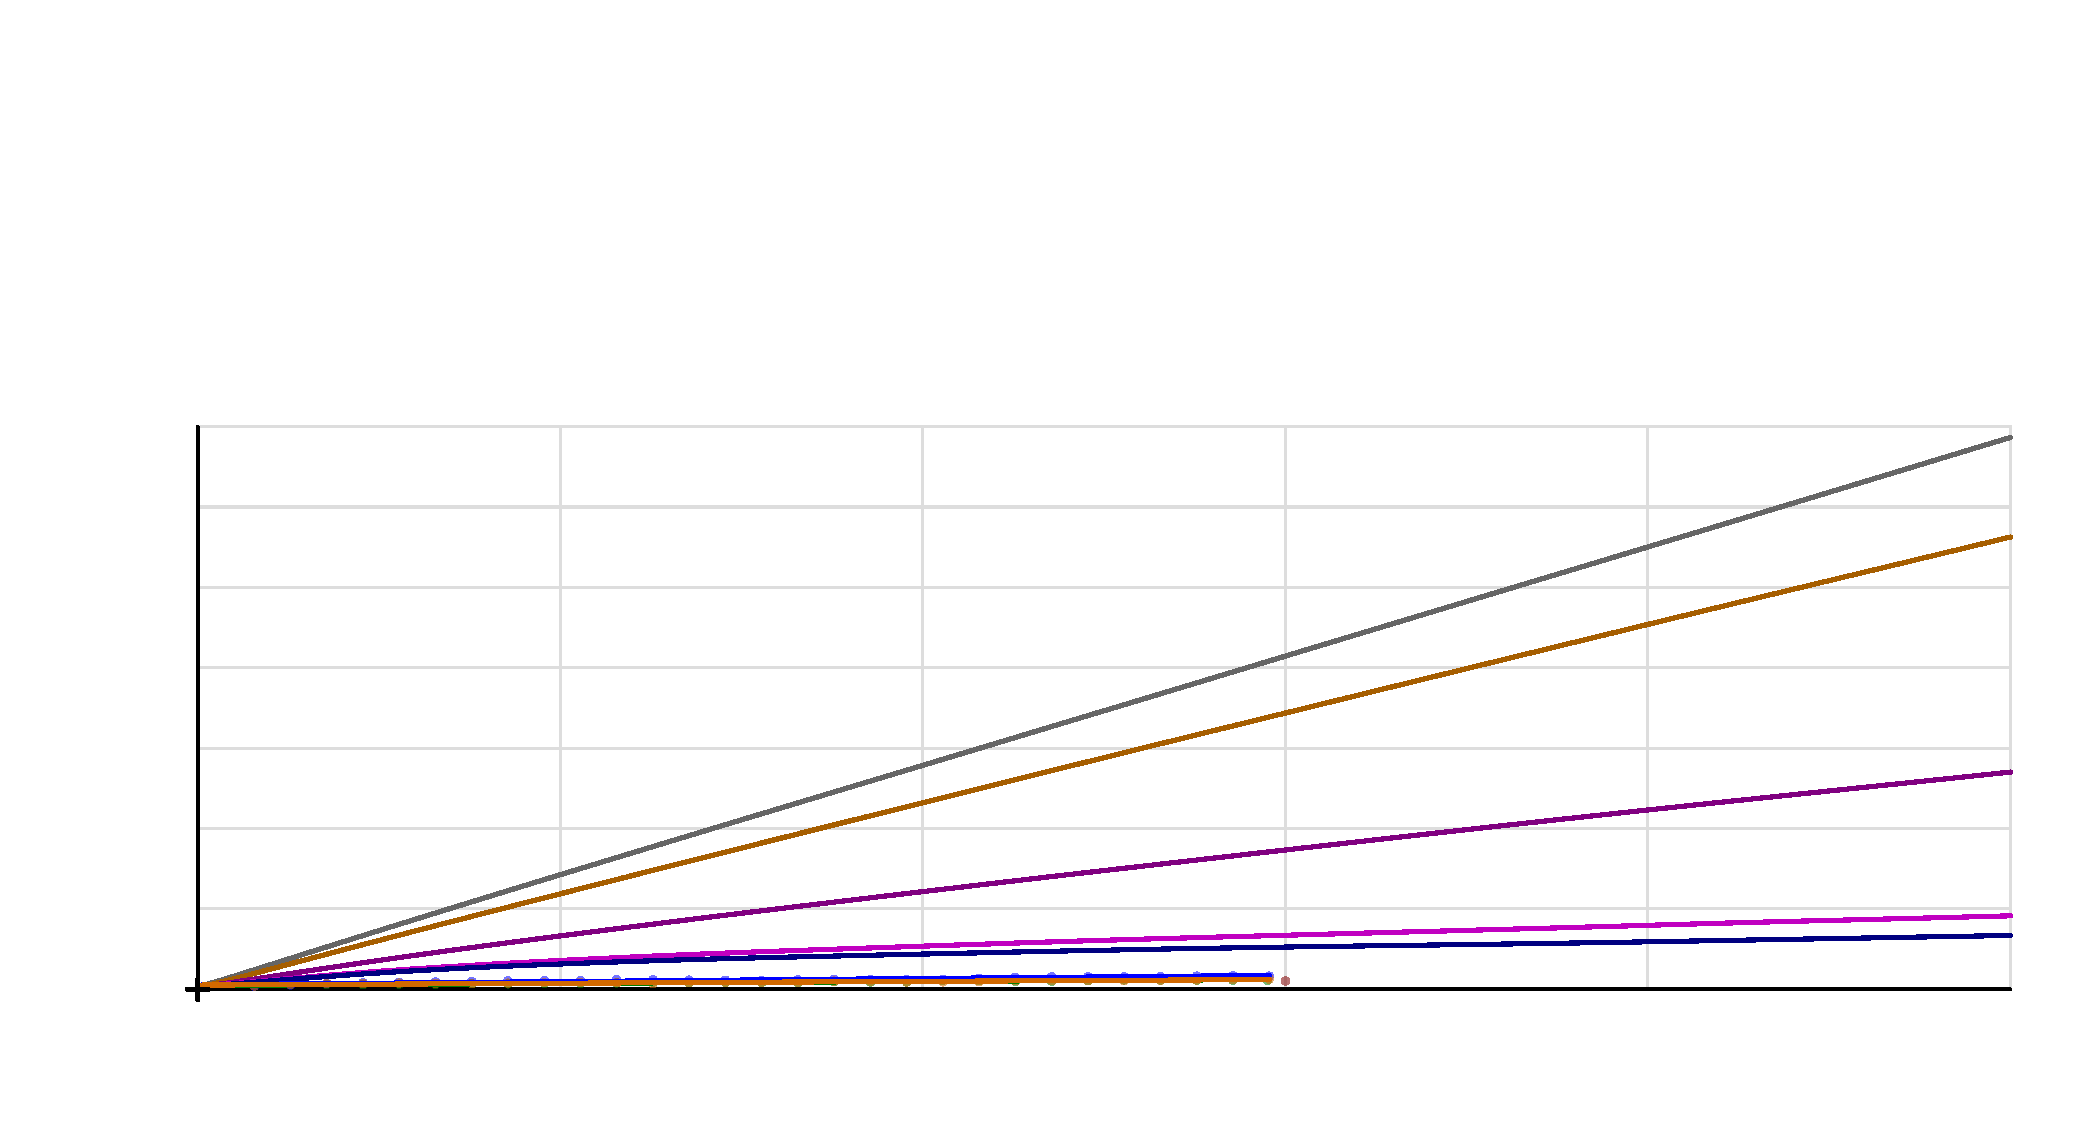
\includegraphics[width=1000.0bp,height=545.0bp]{figures/historical_comparison.pdf}}
\put(95.0,522.0){\makebox(0,0)[lb]{\color{black}\sffamily\fontsize{16}{16}\selectfont HRMS(dAge): frühere Untersuchung und neue Ergebnisse}}
\put(95.0,50.0){\makebox(0,0)[cb]{\color{black}\sffamily\fontsize{12}{12}\selectfont 0}}
\put(269.0,50.0){\makebox(0,0)[cb]{\color{black}\sffamily\fontsize{12}{12}\selectfont 100}}
\put(443.0,50.0){\makebox(0,0)[cb]{\color{black}\sffamily\fontsize{12}{12}\selectfont 200}}
\put(617.0,50.0){\makebox(0,0)[cb]{\color{black}\sffamily\fontsize{12}{12}\selectfont 300}}
\put(791.0,50.0){\makebox(0,0)[cb]{\color{black}\sffamily\fontsize{12}{12}\selectfont 400}}
\put(965.0,50.0){\makebox(0,0)[cb]{\color{black}\sffamily\fontsize{12}{12}\selectfont 500}}
\put(87.0,66.0){\makebox(0,0)[rb]{\color{black}\sffamily\fontsize{12}{12}\selectfont 0}}
\put(87.0,104.57142857142856){\makebox(0,0)[rb]{\color{black}\sffamily\fontsize{12}{12}\selectfont 200}}
\put(87.0,143.1428571428571){\makebox(0,0)[rb]{\color{black}\sffamily\fontsize{12}{12}\selectfont 400}}
\put(87.0,181.71428571428572){\makebox(0,0)[rb]{\color{black}\sffamily\fontsize{12}{12}\selectfont 600}}
\put(87.0,220.28571428571428){\makebox(0,0)[rb]{\color{black}\sffamily\fontsize{12}{12}\selectfont 800}}
\put(87.0,258.8571428571429){\makebox(0,0)[rb]{\color{black}\sffamily\fontsize{12}{12}\selectfont 1000}}
\put(87.0,297.42857142857144){\makebox(0,0)[rb]{\color{black}\sffamily\fontsize{12}{12}\selectfont 1200}}
\put(87.0,336.0){\makebox(0,0)[rb]{\color{black}\sffamily\fontsize{12}{12}\selectfont 1400}}
\put(95.0,500.0){\makebox(0,0)[lb]{\color{red}\sffamily\fontsize{12}{12}\selectfont P23M\_0}}
\put(530.0,500.0){\makebox(0,0)[lb]{\color{green}\sffamily\fontsize{12}{12}\selectfont P23M\_1}}
\put(95.0,478.0){\makebox(0,0)[lb]{\color{blue}\sffamily\fontsize{12}{12}\selectfont UM980}}
\put(530.0,478.0){\makebox(0,0)[lb]{\color[HTML]{d26900}\sffamily\fontsize{12}{12}\selectfont LG290P}}
\put(95.0,456.0){\makebox(0,0)[lb]{\color[HTML]{800000}\sffamily\fontsize{12}{12}\selectfont Alt: präzise Uhren (ein Punkt)}}
\put(95.0,434.0){\makebox(0,0)[lb]{\color[HTML]{666666}\sffamily\fontsize{12}{12}\selectfont Alt: ohne SV-Uhr}}
\put(530.0,434.0){\makebox(0,0)[lb]{\color[HTML]{a65e00}\sffamily\fontsize{12}{12}\selectfont Alt: SV-Uhr}}
\put(95.0,412.0){\makebox(0,0)[lb]{\color[HTML]{800080}\sffamily\fontsize{12}{12}\selectfont Alt: SV-Uhr + Relativität}}
\put(530.0,412.0){\makebox(0,0)[lb]{\color[HTML]{c000c0}\sffamily\fontsize{12}{12}\selectfont Alt: + Ultra-Rapid}}
\put(95.0,390.0){\makebox(0,0)[lb]{\color[HTML]{000080}\sffamily\fontsize{12}{12}\selectfont Alt: + präzise Bahnen}}
\put(530.0,390.0){\makebox(0,0)[lb]{\color{green}\sffamily\fontsize{12}{12}\selectfont P23M\_1: +0.0492 mm/\allowbreak{}s}}
\put(95.0,368.0){\makebox(0,0)[lb]{\color{blue}\sffamily\fontsize{12}{12}\selectfont UM980: +0.0781 mm/\allowbreak{}s}}
\put(530.0,368.0){\makebox(0,0)[lb]{\color[HTML]{d26900}\sffamily\fontsize{12}{12}\selectfont LG290P: +0.0466 mm/\allowbreak{}s}}
\put(103.0,78.0){\makebox(0,0)[lb]{\color{black}\sffamily\fontsize{12}{12}\selectfont (0,0)}}
\put(530.0,12.0){\makebox(0,0)[cb]{\color{black}\sffamily\fontsize{12}{12}\selectfont Korrekturdatenalter dAge [s]}}
\put(19.0,205.0){\rotatebox{90}{\makebox(0,0)[b]{\color{black}\sffamily\fontsize{12}{12}\selectfont Horizontaler RMS-Fehler HRMS [mm]}}}
\end{picture}}
\end{figure}
\begin{figure}[p]\centering
\resizebox{0.98\linewidth}{!}{%
\setlength{\unitlength}{1bp}\begin{picture}(1000.0,523.0)
\put(0,0){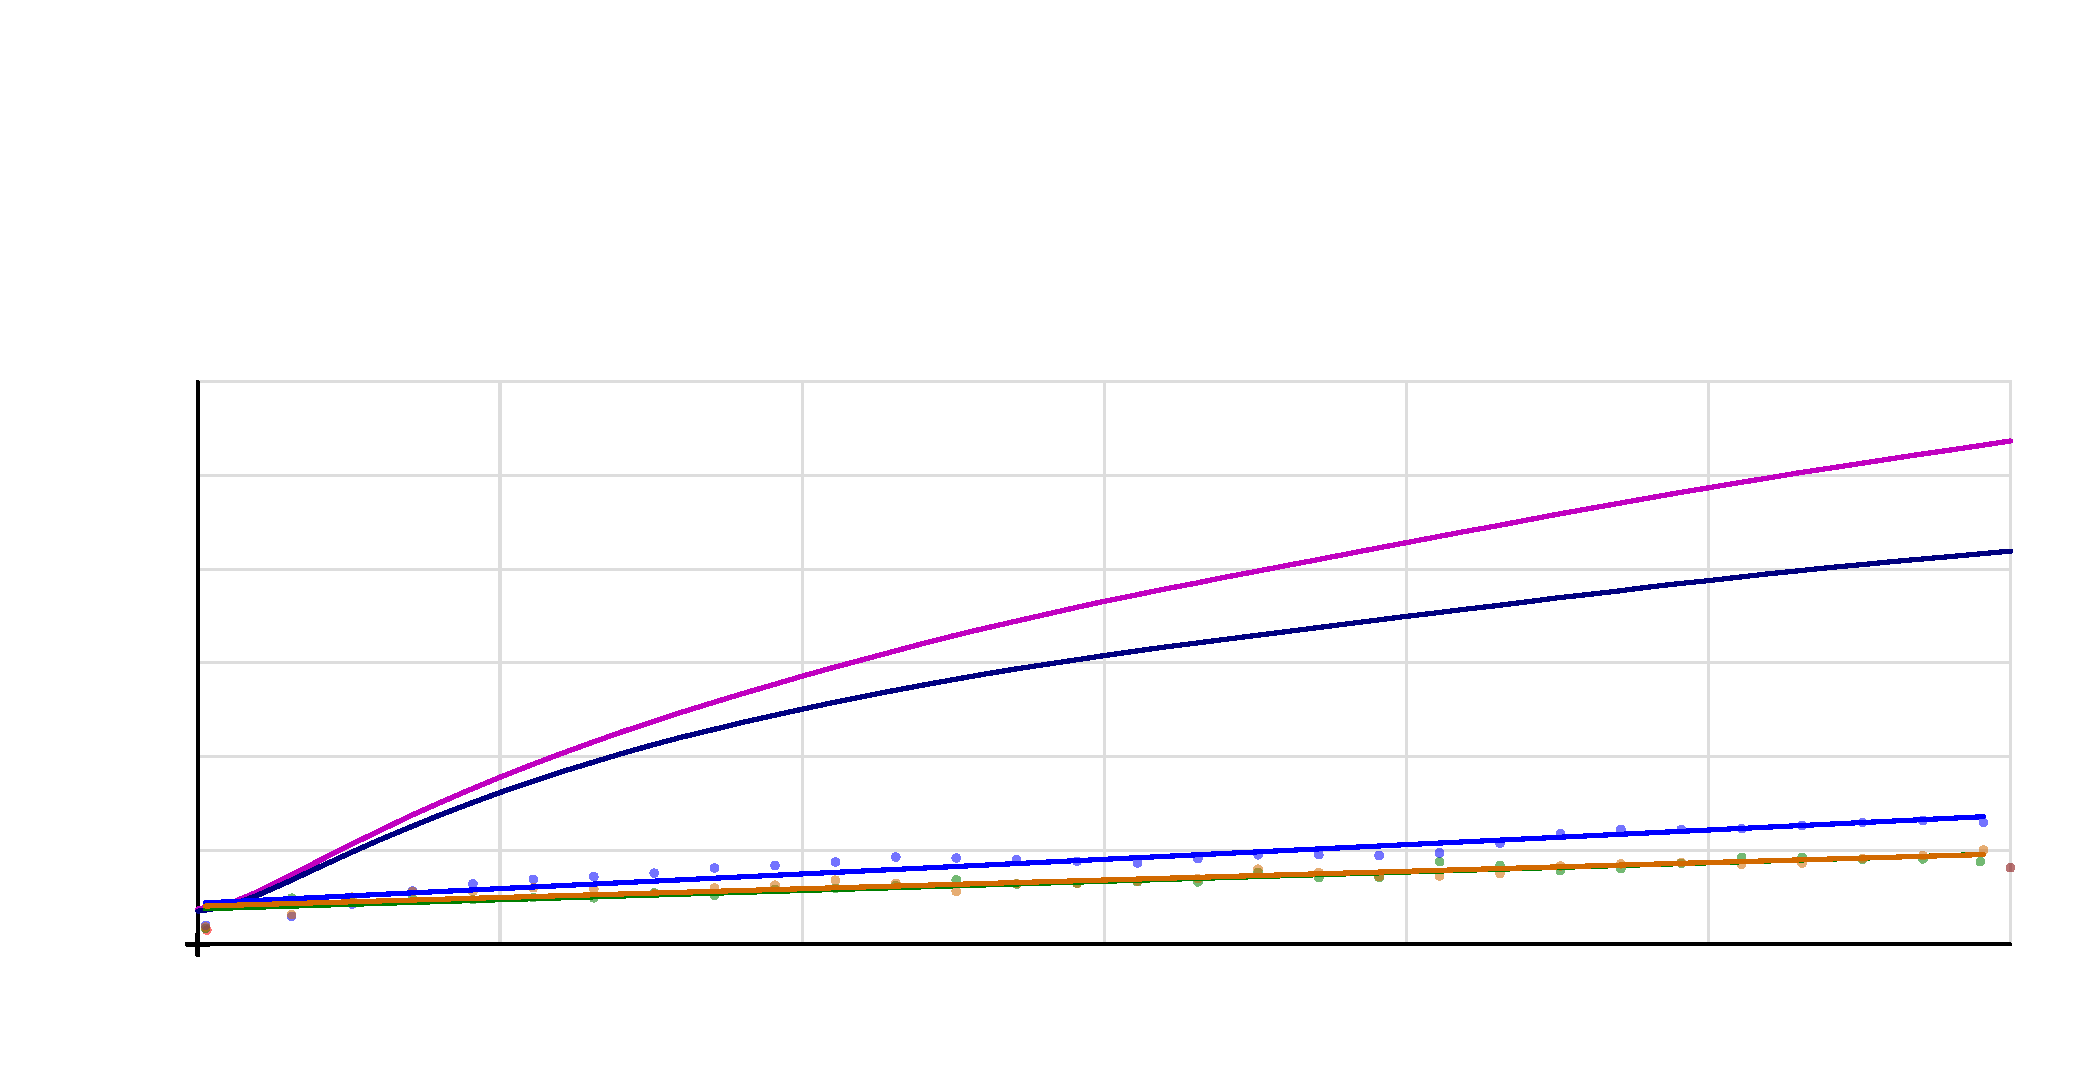
\includegraphics[width=1000.0bp,height=523.0bp]{figures/historical_comparison_detail.pdf}}
\put(95.0,500.0){\makebox(0,0)[lb]{\color{black}\sffamily\fontsize{16}{16}\selectfont HRMS(dAge): Vergleich im Detail (0–300 s, 0–150 mm)}}
\put(95.0,50.0){\makebox(0,0)[cb]{\color{black}\sffamily\fontsize{12}{12}\selectfont 0}}
\put(240.0,50.0){\makebox(0,0)[cb]{\color{black}\sffamily\fontsize{12}{12}\selectfont 50}}
\put(385.0,50.0){\makebox(0,0)[cb]{\color{black}\sffamily\fontsize{12}{12}\selectfont 100}}
\put(530.0,50.0){\makebox(0,0)[cb]{\color{black}\sffamily\fontsize{12}{12}\selectfont 150}}
\put(675.0,50.0){\makebox(0,0)[cb]{\color{black}\sffamily\fontsize{12}{12}\selectfont 200}}
\put(820.0,50.0){\makebox(0,0)[cb]{\color{black}\sffamily\fontsize{12}{12}\selectfont 250}}
\put(965.0,50.0){\makebox(0,0)[cb]{\color{black}\sffamily\fontsize{12}{12}\selectfont 300}}
\put(87.0,66.0){\makebox(0,0)[rb]{\color{black}\sffamily\fontsize{12}{12}\selectfont 0}}
\put(87.0,111.0){\makebox(0,0)[rb]{\color{black}\sffamily\fontsize{12}{12}\selectfont 25}}
\put(87.0,156.0){\makebox(0,0)[rb]{\color{black}\sffamily\fontsize{12}{12}\selectfont 50}}
\put(87.0,201.0){\makebox(0,0)[rb]{\color{black}\sffamily\fontsize{12}{12}\selectfont 75}}
\put(87.0,246.0){\makebox(0,0)[rb]{\color{black}\sffamily\fontsize{12}{12}\selectfont 100}}
\put(87.0,291.0){\makebox(0,0)[rb]{\color{black}\sffamily\fontsize{12}{12}\selectfont 125}}
\put(87.0,336.0){\makebox(0,0)[rb]{\color{black}\sffamily\fontsize{12}{12}\selectfont 150}}
\put(95.0,478.0){\makebox(0,0)[lb]{\color{red}\sffamily\fontsize{12}{12}\selectfont P23M\_0}}
\put(530.0,478.0){\makebox(0,0)[lb]{\color{green}\sffamily\fontsize{12}{12}\selectfont P23M\_1}}
\put(95.0,456.0){\makebox(0,0)[lb]{\color{blue}\sffamily\fontsize{12}{12}\selectfont UM980}}
\put(530.0,456.0){\makebox(0,0)[lb]{\color[HTML]{d26900}\sffamily\fontsize{12}{12}\selectfont LG290P}}
\put(95.0,434.0){\makebox(0,0)[lb]{\color[HTML]{800000}\sffamily\fontsize{12}{12}\selectfont Alt: präzise Uhren (ein Punkt)}}
\put(95.0,412.0){\makebox(0,0)[lb]{\color[HTML]{c000c0}\sffamily\fontsize{12}{12}\selectfont Alt: + Ultra-Rapid}}
\put(530.0,412.0){\makebox(0,0)[lb]{\color[HTML]{000080}\sffamily\fontsize{12}{12}\selectfont Alt: + präzise Bahnen}}
\put(95.0,390.0){\makebox(0,0)[lb]{\color{green}\sffamily\fontsize{12}{12}\selectfont P23M\_1: +0.0492 mm/\allowbreak{}s}}
\put(530.0,390.0){\makebox(0,0)[lb]{\color{blue}\sffamily\fontsize{12}{12}\selectfont UM980: +0.0781 mm/\allowbreak{}s}}
\put(95.0,368.0){\makebox(0,0)[lb]{\color[HTML]{d26900}\sffamily\fontsize{12}{12}\selectfont LG290P: +0.0466 mm/\allowbreak{}s}}
\put(103.0,78.0){\makebox(0,0)[lb]{\color{black}\sffamily\fontsize{12}{12}\selectfont (0,0)}}
\put(530.0,12.0){\makebox(0,0)[cb]{\color{black}\sffamily\fontsize{12}{12}\selectfont Korrekturdatenalter dAge [s]}}
\put(19.0,205.0){\rotatebox{90}{\makebox(0,0)[b]{\color{black}\sffamily\fontsize{12}{12}\selectfont Horizontaler RMS-Fehler HRMS [mm]}}}
\end{picture}}
\end{figure}\clearpage
\clearpage\section{English — Turn-table test — 2026-11-07}

\begin{quote}\ttfamily\footnotesize python3 analysis/\allowbreak{}turn\_table.py --dataset datasets/\allowbreak{}2026-11-07\\python3 analysis/\allowbreak{}build\_report.py --dataset datasets/\allowbreak{}2026-11-07\end{quote}

\subsection{Setup and method}

P23M\_0 is the continuously corrected reference, inferred from {\small\texttt{P23M\_\allowbreak{}continious.nmea}}. P23M\_1, UM980 and LG290P are the three outage receivers. A shared rotating antenna setup as in the previous experiment is assumed as requested. Firmware versions and independently logged outage switching times are unavailable.

The same method as on 2026-11-03 is used: local WGS84 coordinates, robust geometric circle fitting, reference-derived time-aligned angles, and RTK-fixed positions only (GGA quality 4). P23M\_0 provides approximately 10 Hz, the outage receivers approximately 1 Hz. Alignment uses UTC measurement epochs without fitted time shifts. The reference circle uses its full available fixed recording. Reference interpolation is limited to gaps of at most 3 s.

RMC dates in all three outage files confirm 2026-11-07; the same day is assumed for P23M\_0, which has no RMC date. Each outage file has 13,096 positions on a complete 1-s grid. {\small\texttt{P23M\_\allowbreak{}outages.nmea}} contains 45 corrupted sentences rejected for invalid checksums, without gaps in its valid position grid. The other files have no detected checksum/\allowbreak{}field errors. There are no duplicate position epochs.

\subsection{Circle and rotation}

Radius: \textbf{0.304865 m}. Common interval: \textbf{01:40:13–05:18:28 UTC}. Mean rotation period: \textbf{181.215 s}, from \textbf{72 complete revolutions}; standard deviation \textbf{9.240 s}, minimum \textbf{172.530 s}, maximum \textbf{247.429 s}. There is one continuous reliable reference segment. Of 131,115 fixed reference positions, one radial outlier is excluded from angle estimation; 130,915 reference positions are retained within the common interval. Incomplete revolutions are excluded.

\subsection{Errors across all retained fixed epochs}

\begin{center}\small\begin{tabular}{lrrrr}\toprule
Receiver & Epochs & HRMS [mm] & 95th percentile [mm] & Maximum [mm]\\\midrule
P23M\_0 & 130915 & 3.75 & 7.58 & 16.12\\
P23M\_1 & 12742 & 13.90 & 28.53 & 58.91\\
UM980 & 12790 & 18.93 & 35.40 & 92.51\\
LG290P & 12732 & 14.22 & 29.27 & 67.27\\
\bottomrule\end{tabular}\end{center}

\subsection{Common outage comparison}

The fair comparison uses \textbf{7,655 identical UTC epochs} where all three outage receivers are RTK-fixed and each reports dAge >10 s. The reference is not an outage candidate. This requires three simultaneously valid outage receivers, compared with two in the November 3 experiment.

\begin{center}\small\begin{tabular}{lrrrr}\toprule
Receiver & HRMS [mm] & Median [mm] & 95th percentile [mm] & Maximum [mm]\\\midrule
P23M\_1 & 17.59 & 13.74 & 32.26 & 58.91\\
UM980 & 24.06 & 18.44 & 41.59 & 92.51\\
LG290P & 17.84 & 14.08 & 32.27 & 55.61\\
\bottomrule\end{tabular}\end{center}

P23M\_1 has the lowest RMS and median; its 95th percentile is practically identical to LG290P. LG290P has the lowest maximum error within this common selection. The RMS difference between P23M\_1 and LG290P is only about 0.25 mm (1.4\%); without an uncertainty analysis this does not establish a reliable general ranking. UM980 has larger typical outage errors in this experiment.

\subsection{HRMS versus dAge and linear fits}

The full scatter plot precedes the HRMS/\allowbreak{}fit plot, with errors in millimetres. HRMS is computed in 10-s intervals (0,10], (10,20], etc.; zero age belongs to the first interval. Points use the mean observed age. Bin HRMS values receive equal weight in a straight-line fit with a free intercept. Lines stop at observed ages. This table uses each receiver’s retained fixed epochs independently, without a common-epoch selection.

\begin{center}\small\begin{tabular}{lrrrr}\toprule
Receiver & ≤10 s [mm] & 170–180 s [mm] & 290–300 s [mm] & Slope [mm/\allowbreak{}s]\\\midrule
P23M\_1 & 4.23 & 19.18 & 22.01 & 0.04924\\
UM980 & 5.02 & 23.81 & 32.52 & 0.07812\\
LG290P & 4.59 & 20.02 & 25.11 & 0.04664\\
\bottomrule\end{tabular}\end{center}

The reference occupies only the first age bin, so its HRMS slope cannot be estimated. P23M\_1 ends at 299 s (last-bin mean age 295.0 s); UM980 and LG290P reach 300 s (mean 295.5 s). LG290P has the lowest fitted slope, but P23M\_1 has the lower observed HRMS in the last interval. Slope and error level measure different properties.

\subsection{Assessment against the earlier study (steps 1–6)}

Full and detailed plots overlay current bins and fits with reconstructed curves from Figure 1, page 2 of references/\allowbreak{}historical-outage-results/\allowbreak{}original.pdf. Historical coordinates are approximate plotted values, not raw observations. Historical numbers below refer approximately to 300 s; current numbers are measured RMS values in 290 < dAge ≤300 s, not fit predictions.

\textbf{1. Use outdated reference data unchanged:} Earlier HRMS was about 829 mm. Current 22.0–32.5 mm results are substantially lower. Correction age alone does not determine accuracy; modelling and experimental conditions matter.

\textbf{2. Apply broadcast satellite clock models:} Earlier HRMS was about 687 mm. Satellite clock evolution matters, but the simple model alone was insufficient in the earlier experiment.

\textbf{3. Add the relativistic correction:} Earlier HRMS was about 347 mm. Model terms that largely cancel for simultaneous observations become relevant when reference and rover epochs differ.

\textbf{4. Use ultra-rapid orbits and clocks:} Earlier HRMS was about 134 mm. Improved satellite information substantially reduced errors. Current results are lower, but the reason cannot be identified without a controlled model comparison.

\textbf{5. Use final precise orbits:} Earlier HRMS was about 105 mm. The additional improvement was limited: orbit errors alone did not explain the residual.

\textbf{6. Use final precise satellite clocks:} Earlier HRMS was about 20 mm at 300 s. Current P23M\_1 at 22.0 mm and LG290P at 25.1 mm are of the same order; UM980 reaches 32.5 mm. The historical point uses precise products available after the experiment and does not define a universal real-time limit.

\textbf{What do we learn?} Residual errors are small and increase with dAge, consistent with a contribution from time-dependent satellite errors. The earlier report makes short-term satellite clock nonlinearity a useful hypothesis to test, not a cause established by NMEA positions alone. Current internal correction models are unknown. These results do not establish a physical accuracy limit.

Near 300 s, HRMS values are lower than on November 3: earlier P23A\_1 was 34.2 mm and UM980 36.2 mm; now P23M\_1 is 22.0 mm, UM980 32.5 mm and LG290P 25.1 mm. This comparison is descriptive: P23M and P23A are differently named receivers, circle radius and rotation differ, and the date, satellite geometry and common selection are not identical. An isolated hardware improvement is not established.

\textbf{Limits and next verification:} Expected positions come from P23M\_0 and the fitted circle. Its tangential error and shared systematic errors are not independently observable. Statistics concern retained fixed solutions, not full outage availability or absolute accuracy. A controlled follow-up would process the same raw observations with different clock/\allowbreak{}orbit models, independent position truth and a separate availability assessment.

\subsection{Why centimetre accuracy is possible today with broadcast products}

\textbf{Historical context:} The earlier experiment dates to \textbf{18 July 2005}, using \textbf{Trimble receivers in GPS-only operation}. Date and receiver family were supplied by the project owner; the PDF creation date in 2026 is not the acquisition date. [R1] Broadcast-only operation in the current experiment is also supplied setup information. NMEA position outputs do not record the complete receiver configuration.

\subsubsection{Temporal residual change matters more than absolute error}

An absolute broadcast orbit or clock error does not enter relative RTK at its full magnitude. For a short baseline, a schematic temporal contribution is {\small\texttt{r\_\allowbreak{}s(t) \ensuremath{\approx} e\_\allowbreak{}s(t) - e\_\allowbreak{}s(t0)}}, where e\_s is the remaining combined satellite-related range error after broadcast modelling; satellite differencing and geometric projections also apply. A large, almost constant component can largely cancel, while a smaller rapidly changing error can matter more.

If its development is estimated before the outage and propagated, the prediction residual matters: {\small\texttt{r\_\allowbreak{}s(t) \ensuremath{\approx} e\_\allowbreak{}s(t) - e\_\allowbreak{}s(t0) - Δe\_\allowbreak{}pred,s(t)}}. This illustrates the principle, not any tested receiver's unknown source code. Better absolute final orbits are therefore not automatically the most effective improvement here. This agrees with step 5 of the 2005 report, where better orbits alone produced limited additional benefit. [R1]

\subsubsection{The rover retains its initialisation and continues receiving satellites}

A base-data link outage is not a satellite-signal outage. The rover still observes current carrier phases and starts from an initialised solution with resolved ambiguities and estimated error parameters. States can be propagated; each epoch does not restart as unaided single-point positioning. Our position files cannot identify whether an implementation predicts individual clock states, observation models or other combined states.

Quectel describes RTK HOLD as observation-model prediction; Unicore describes RTKKEEP as modelling and parameter estimation for orbit, clock and atmospheric effects. These document available functions, not their exact implementation, activation or universally applicable accuracy in the firmware tested. Comparable internal algorithm documentation for FMI is unavailable here. \href{https://www.quectel.com/product/gnss-lg290p/}{R5} \href{https://en.unicorecomm.com/core-technology/}{R6}

\subsubsection{Satellite populations and short-term clock stability have changed}

Galileo uses passive hydrogen masers among its onboard clocks. Better short-term stability reduces unpredictable change during an outage; this does not imply every modern satellite is always better. \href{https://www.esa.int/Applications/Satellite_navigation/How_the_Galileo_atomic_clocks_work}{R7}

Shu et al. report approximately 11.2 mm for GPS versus 3.0 mm for Galileo in combined broadcast residual changes over 15 s. These are satellite-related range errors, not position HRMS or a 300-s extrapolation. They support the temporal-error mechanism, not a universal 300-s guarantee. \href{https://doi.org/10.3390/rs11101256}{R2}

\subsubsection{More suitable observations and multi-frequency processing}

Our three outage receivers each report a \textbf{median of 42 satellites} in fixed GGA sentences: ranges are 35–46 for P23M\_1 and UM980 and 36–46 for LG290P. These are measurements from our files. They do not identify the constellations, frequencies or weights actually used in the outage solution. The reference reports zero throughout this GGA field, so it cannot be used as a reference satellite count.

Additional suitable observations can improve geometry, fault detection and selection of stable signals. Correlations and systematic errors prevent a blanket 1/\allowbreak{}sqrt(N) accuracy improvement. Selection can matter as much as observation count.

The 2005 experiment already used an ionosphere-free combination; it was not a simple single-frequency comparison. For classical GPS L1/\allowbreak{}L2, equal independent phase noise and coefficients near 2.546 and -1.546 imply a calculated noise amplification of about \textbf{2.98}. Modern multi-frequency processing permits other combinations and estimation models, but their use here is unverified. Additional frequencies alone do not remove frequency-independent satellite clock errors. \href{https://gssc.esa.int/navipedia/index.php?title=Combination_of_GNSS_Measurements}{R8}

\textbf{Interpretation:} The most plausible explanation combines more favourable temporal satellite errors, more suitable observations and better propagation of estimated states. Their individual quantitative contributions cannot be identified from these NMEA positions. The 2005 20-mm point is neither a current physical limit nor an established real-time bound.

\subsection{Comparable published work and strength of evidence}

\textbf{Bhandari, O’Keefe and Lachapelle (2013):} Investigate multi-GNSS RTK correction outages from seconds to many minutes. This establishes longstanding prior work; the abstract does not validate our specific 300-s HRMS values. \href{https://www.ion.org/publications/abstract.cfm?articleID=11153}{R3}

\textbf{Du et al. (2019):} Table 3 reports dynamic real-time-scenario component standard deviations below 3 cm for E/\allowbreak{}N over 20 min and U over 15 min. Precise/\allowbreak{}final or ultra-rapid products are used; component standard deviations are not horizontal RMS and this is not broadcast-only replication. \href{https://doi.org/10.3390/s19153376}{R4}

\textbf{Shu et al. (2019):} The short-delay results above explain constellation differences. They support a temporal residual-error hypothesis, but different delays and experiments prevent direct accuracy transfer. \href{https://doi.org/10.3390/rs11101256}{R2}

\textbf{Quectel and Unicore:} Describe RTK HOLD/\allowbreak{}KEEP for minute-long outages. These are manufacturer function descriptions, not independent confirmation of the centimetre values measured here. \href{https://www.quectel.com/product/gnss-lg290p/}{R5} \href{https://en.unicorecomm.com/core-technology/}{R6}

\textbf{NovAtel RTK ASSIST:} The SMART7 manual quotes typical 4 cm and bridging up to 20 min, using additional TerraStar L-band corrections. This is a different architecture, not evidence for equivalent performance without further corrections. \href{https://docs.novatel.com/OEM7/Content/PDFs/PreviousVersions/SMART7_Installation_Operation_Manual_v10.pdf}{R9}

\textbf{Novelty:} We are not the first to obtain centimetre solutions during RTK correction outages. No independently verified, method-matched comparison of FMI P23A/\allowbreak{}M, UM980 and LG290P was identified in this search. No world-first or market-leadership claim follows.

\subsection{Assessment of FMI–FEYMAN P23A/\allowbreak{}M versus UM980 and LG290P}

The table separates distinct metrics. HRMS, 95th percentile and maximum use 7,655 common fixed epochs with dAge >10 s. The last age interval and fitted slopes use each receiver's fixed epochs separately. Fixed fractions use all 13,096 valid epochs in the complete 1-Hz recording, not outages alone.

\begin{center}\small\begin{tabular}{lrrr}\toprule
Metric & FMI P23M\_1 & UM980 & LG290P\\\midrule
Common HRMS [mm] & 17.59 & 24.06 & 17.84\\
95th percentile [mm] & 32.26 & 41.59 & 32.27\\
Common maximum [mm] & 58.91 & 92.51 & 55.61\\
HRMS 290–300 s [mm] & 22.01 & 32.52 & 25.11\\
Slope [mm/\allowbreak{}s] & 0.0492 & 0.0781 & 0.0466\\
Whole-record fixed [\%] & 97.30 & 97.66 & 97.22\\
\bottomrule\end{tabular}\end{center}

\textbf{Against Unicore UM980:} FMI P23M\_1 has about \textbf{26.9\% lower common outage HRMS} and \textbf{32.3\% lower HRMS in the last age interval}. Its 95th percentile and common maximum are also lower. Retained-fixed accuracy is clearly more favourable here. UM980 nevertheless reports a slightly higher fixed fraction across the whole recording; smaller error and greater availability are different objectives.

\textbf{Against Quectel LG290P:} P23M\_1's common HRMS is only \textbf{0.25 mm, or 1.4\%, lower}, with an essentially identical 95th percentile. LG290P has the smaller common maximum and fitted slope; FMI has the lower measured HRMS near 300 s. This is a close, competitive result, not a reliable general victory over LG290P. No significance analysis was performed.

\textbf{P23A on 3 November 2026:} On 6,812 common epochs, HRMS was 18.85 mm versus UM980's 26.85 mm, about 29.8\% lower. FMI's maximum event was larger then: 96.47 versus 79.39 mm. Both local experiments show favourable typical FMI errors against UM980, not universal superiority on every criterion.

\textbf{Development progress:} The earlier discussion is now available as a ChatGPT implementation note dated \textbf{18 October 2026}. Page 11 discusses an approximate position change of \textbf{0.36 m over 120 s}, or \textbf{3 mm/\allowbreak{}s}. This documents the earlier discussion and its scale, not an independently verifiable FMI HRMS series or firmware attribution. The next section separates that observation from current metrics. P23A on November 3 versus P23M on November 7 likewise cannot isolate firmware progress because device labels, dates, radii and selections differ. [R10]

\textbf{Reference dependence:} Both reference receivers are themselves FMI units. Shared manufacturer- or model-dependent errors might cancel more strongly in an FMI-versus-FMI comparison; whether this occurs here is unproven. A manufacturer-neutral absolute ranking requires independent position/\allowbreak{}angle truth. Fixed status is not an integrity guarantee. Whole-record fixed fractions do not replace analysis of actual outage availability, recovery time or incorrect fixes.

\textbf{Verdict for this test:} FMI P23M delivers very competitive retained-fixed accuracy, close to LG290P and with smaller typical outage errors than UM980. This demonstrates a strong development state and describes this experiment defensibly; it is not yet a general product or market ranking.

\subsection{Relation to the ChatGPT report dated 18 October 2026}

[R10] is a \textbf{14-page AI-generated technical implementation note}, not an independent comparative experiment. Its companion JPG is a conceptual workflow diagram. The project owner associates these documents with the earlier FMI outage discussion, but the PDF itself contains no raw series unambiguously attributed to an FMI model and firmware version.

\subsubsection{What the discussed 0.36 m actually establishes}

Page 11, equation 11.1, discusses approximately 0.36 m of position change over 120 s: \textbf{3 mm/\allowbreak{}s or 18 cm/\allowbreak{}min}. It explicitly treats this as a discussed scale, not a raw-data-derived HRMS statistic or measured satellite clock error. Its approximately 1.20 ns range-equivalent value is a speed-of-light conversion, not a direct clock observation.

For scale only, current measurements in \textbf{110 < dAge ≤120 s} are shown below. Each receiver has 270 retained fixed epochs with mean age 115.5 s. These are HRMS values over multiple epochs, not the displacement of an individual position curve.

\begin{center}\small\begin{tabular}{lrr}\toprule
Receiver & HRMS 110–120 s [mm] & Epochs\\\midrule
P23M\_1 & 15.63 & 270\\
UM980 & 23.23 & 270\\
LG290P & 16.23 & 270\\
\bottomrule\end{tabular}\end{center}

Dividing the previously discussed 360 mm by these HRMS values would \textbf{not establish a defensible improvement factor}. Nor is the previous average position-change rate of 3 mm/\allowbreak{}s equivalent to today's slope of binned HRMS versus age. Current small errors are consistent with substantially more favourable behaviour, but the original observations, ground truth, signal/\allowbreak{}firmware configuration and exact meaning of 0.36 m are unavailable for a controlled before/\allowbreak{}after test.

\subsubsection{Technical checks documented in the note}

\textbf{Full satellite clock change:} Sections 3–5 evaluate clock models at the relevant transmission times with consistent time scales and differencing direction. For {\small\texttt{D\_\allowbreak{}s = clock\_\allowbreak{}model(u1) - clock\_\allowbreak{}model(u0)}}, add \textbf{+c*D\_s} to the raw asynchronous difference. An algebraic adjustment on the old reference side alone uses \textbf{-c*D\_s}. The polynomial and periodic relativistic terms must be applied completely and exactly once under the constellation's conventions. Sign, unit, transmit/\allowbreak{}receive-time and double-correction mistakes are plausible failure modes, not established historical FMI causes.

\textbf{Synthetic reference prediction needs more than a clock correction:} Section 6 includes changes in satellite geometry, atmosphere and other carrier terms, plus a consistent treatment of the common reference clock. A stationary base antenna does not imply constant satellite ranges. Predicted reference values are correlated model quantities, not independently observed fresh RTCM data.

\textbf{Delta-phase alone does not remove systematic errors:} Section 7.3 gives the raw-observation identity between old-reference processing and delta-phase anchored at the last RTK fix. With the same information and consistent statistics, these rearrange the same data. Small successive steps do not erase systematic clock changes: their sum is the total change between endpoints. Switching to delta-phase alone therefore cannot guarantee today's centimetre performance.

\textbf{Uncertainty and continuity are part of the model:} Sections 8–10 address shared anchor epochs, cross-covariances, cycle slips, navigation changes and recovery. They support independent accuracy validation rather than treating fixed status as an integrity guarantee.

\subsubsection{How this changes the assessment}

The earlier discussion is now available as a document and is no longer described as wholly missing. It records a discussed problem scale and specific modelling questions. It does \textbf{not} identify which change was actually implemented in FMI or establish that a particular sign/\allowbreak{}relativity fix caused current performance. Figures on pages 12–13 reproduce historical material; they are not additional FMI measurement series acquired on October 18. The clock plot is the same comparison as [R1], whose date and Trimble GPS-only context are now known.

The FMI assessment remains positive: November data demonstrate small, competitive retained-fixed errors against simultaneously recorded competitors. A qualitative description of progress relative to the earlier discussion is understandable. Quantifying firmware progress requires the earlier raw observations and versions or a controlled replay experiment.

\subsection{Follow-up experiments that can separate the causes}

Repeat GPS-only and multi-GNSS runs with the same modern receivers under comparable conditions, separating constellations where possible. Record raw observations, RTCM streams, firmware versions, signal groups and enabled correction/\allowbreak{}hold functions. Use independent truth and logged switching times; assess errors, fixed availability, incorrect fixes and recovery separately. Repeat across days, baselines and dynamics. Evaluate uncertainty over complete outage cycles rather than treating correlated seconds as independent repetitions.

\subsection{References and evidence status}

Sources checked on 7 November 2026. Research, manufacturer claims and our measurements have different evidential roles; none exactly replicates this experiment.

\textbf{[R1]} Sören Klose. Frühere Outage Results. Trimble GPS-only; measurement 18 July 2005 (project-owner context). Files: {\small\texttt{original.docx}}, {\small\texttt{original.pdf}}. Folder: references/\allowbreak{}historical-outage-results/\allowbreak{}.

\textbf{[R2]} Bao Shu et al. (2019). \href{https://doi.org/10.3390/rs11101256}{Analysis of Factors Affecting Asynchronous RTK Positioning with GNSS Signals}. peer-reviewed; Remote Sensing 11(10), 1256. DOI: \href{https://doi.org/10.3390/rs11101256}{10.3390/\allowbreak{}rs11101256}.

\textbf{[R3]} V. Bhandari, K. O’Keefe, G. Lachapelle (2013). \href{https://www.ion.org/publications/abstract.cfm?articleID=11153}{Assessment of Multi-constellation RTK Solutions During Differential Correction Data Outages}. research conference; ION GNSS+ 2013, pp. 3194–3204.

\textbf{[R4]} Yuan Du et al. (2019). \href{https://doi.org/10.3390/s19153376}{A New Asynchronous RTK Method to Mitigate Base Station Observation Outages}. peer-reviewed; Sensors 19(15), 3376. DOI: \href{https://doi.org/10.3390/s19153376}{10.3390/\allowbreak{}s19153376}; full text: https:/\allowbreak{}/\allowbreak{}pmc.ncbi.nlm.nih.gov/\allowbreak{}articles/\allowbreak{}PMC6696619/\allowbreak{}.

\textbf{[R5]} Quectel (accessed 2026-11-07). \href{https://www.quectel.com/product/gnss-lg290p/}{LG290P series: RTK HOLD and multi-constellation support}. manufacturer documentation, not independent validation.

\textbf{[R6]} Unicore (accessed 2026-11-07). \href{https://en.unicorecomm.com/core-technology/}{Core Technology: RTKKEEP}. manufacturer documentation, not independent validation.

\textbf{[R7]} European Space Agency (accessed 2026-11-07). \href{https://www.esa.int/Applications/Satellite_navigation/How_the_Galileo_atomic_clocks_work}{How the Galileo atomic clocks work}. technical background.

\textbf{[R8]} J. Sanz Subirana, J. M. Juan Zornoza, M. Hernández-Pajares (2011). \href{https://gssc.esa.int/navipedia/index.php?title=Combination_of_GNSS_Measurements}{Combination of GNSS Measurements}. ESA Navipedia technical reference.

\textbf{[R9]} NovAtel (User Manual v10; accessed 2026-11-07). \href{https://docs.novatel.com/OEM7/Content/PDFs/PreviousVersions/SMART7_Installation_Operation_Manual_v10.pdf}{SMART7 Installation and Operation User Manual, section 3.9, page 47: RTK ASSIST}. manufacturer documentation; uses additional TerraStar L-band corrections.

\textbf{[R10]} ChatGPT. GNSS Positioning During Reference Data Outages: Observation models, clock propagation and implementation. Technical implementation note, 18 October 2026, 14 pp.; especially pp. 3–8 and 11–14. Local file: {\small\texttt{2026-10-18.gnss-reference-outage.pdf}} in references/\allowbreak{}literature/\allowbreak{}. AI-generated discussion, not an independent FMI benchmark.

\begin{figure}[p]\centering
\resizebox{0.98\linewidth}{!}{%
\setlength{\unitlength}{1bp}\begin{picture}(680.0,715.0)
\put(0,0){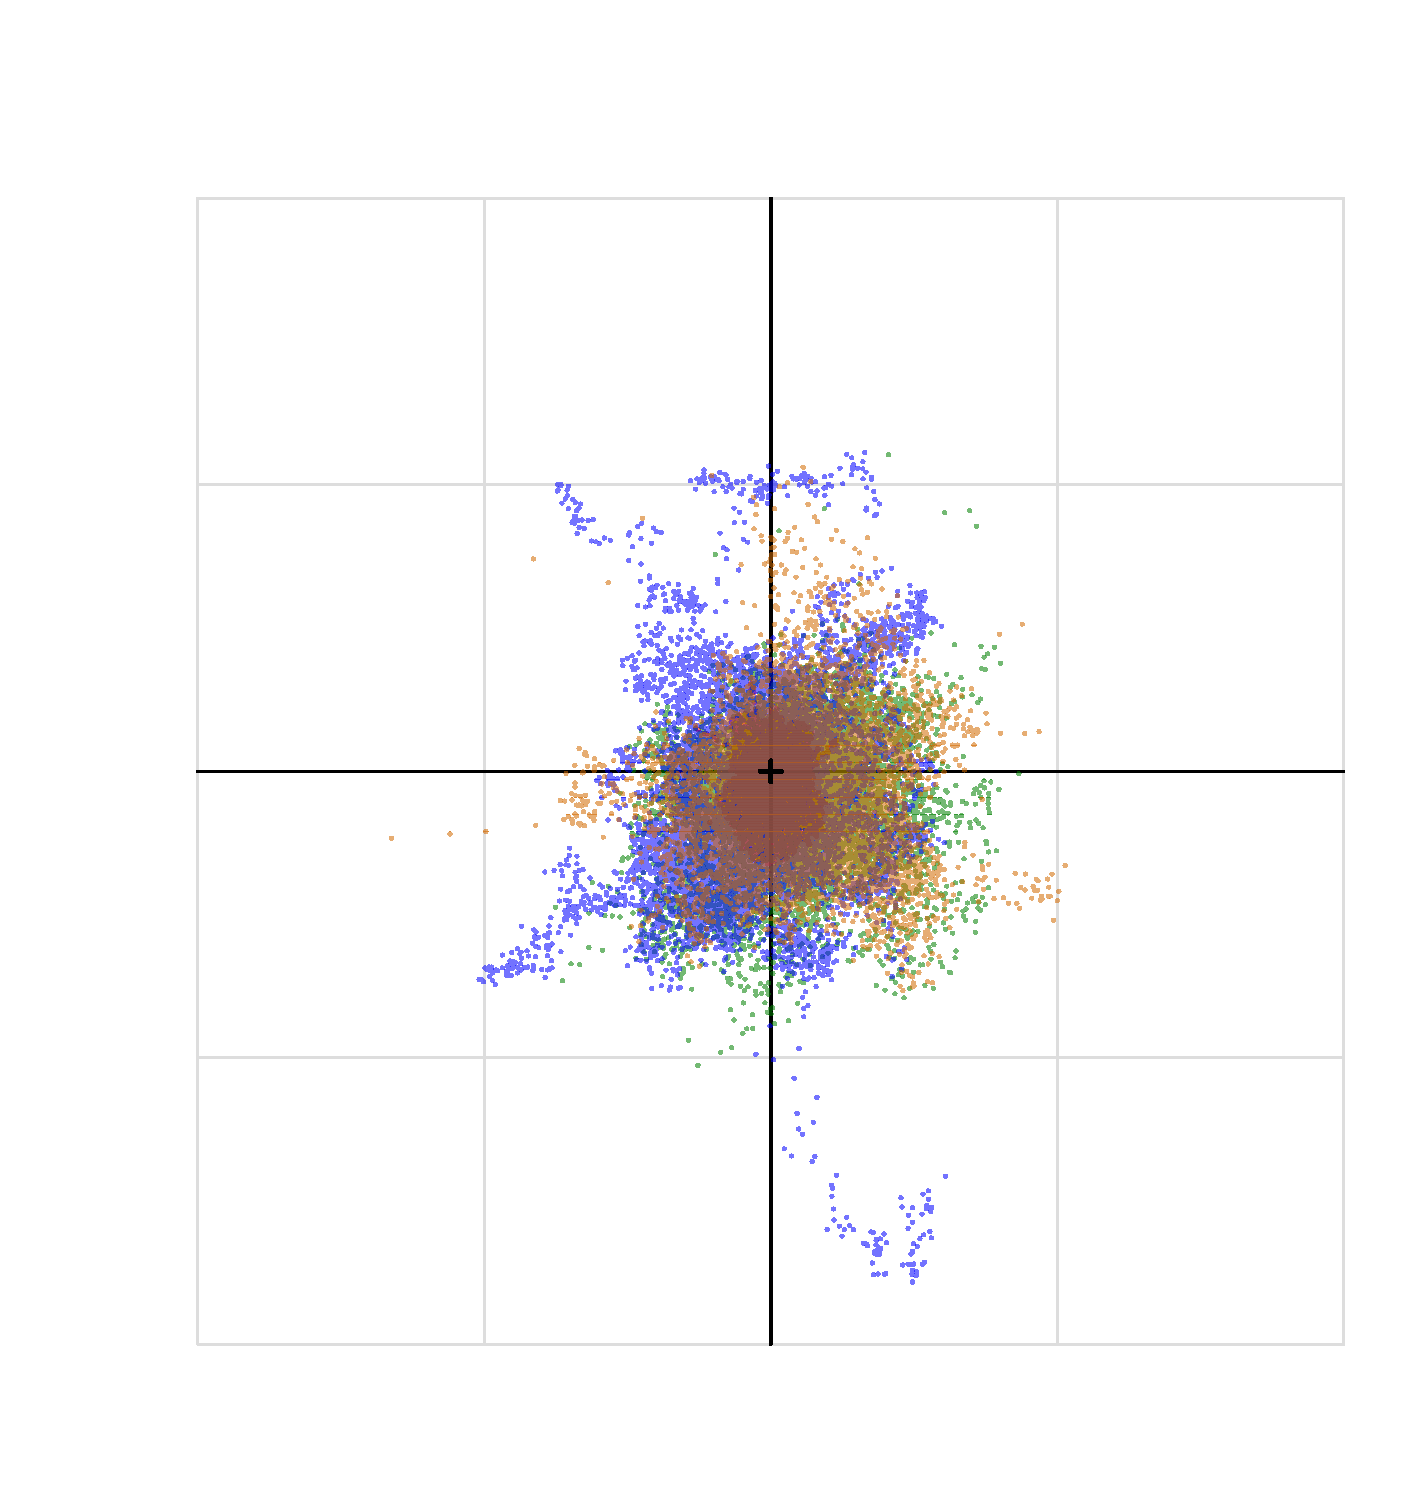
\includegraphics[width=680.0bp,height=715.0bp]{figures/horizontal_en.pdf}}
\put(95.0,692.0){\makebox(0,0)[lb]{\color{black}\sffamily\fontsize{16}{16}\selectfont Horizontal errors relative to the time-aligned expected circle}}
\put(95.0,50.0){\makebox(0,0)[cb]{\color{black}\sffamily\fontsize{12}{12}\selectfont -0.1}}
\put(232.5,50.0){\makebox(0,0)[cb]{\color{black}\sffamily\fontsize{12}{12}\selectfont -0.05}}
\put(370.0,50.0){\makebox(0,0)[cb]{\color{black}\sffamily\fontsize{12}{12}\selectfont 0}}
\put(507.50000000000006,50.0){\makebox(0,0)[cb]{\color{black}\sffamily\fontsize{12}{12}\selectfont 0.05}}
\put(645.0,50.0){\makebox(0,0)[cb]{\color{black}\sffamily\fontsize{12}{12}\selectfont 0.1}}
\put(87.0,66.0){\makebox(0,0)[rb]{\color{black}\sffamily\fontsize{12}{12}\selectfont -0.1}}
\put(87.0,203.5){\makebox(0,0)[rb]{\color{black}\sffamily\fontsize{12}{12}\selectfont -0.05}}
\put(87.0,341.0){\makebox(0,0)[rb]{\color{black}\sffamily\fontsize{12}{12}\selectfont 0}}
\put(87.0,478.50000000000006){\makebox(0,0)[rb]{\color{black}\sffamily\fontsize{12}{12}\selectfont 0.05}}
\put(87.0,616.0){\makebox(0,0)[rb]{\color{black}\sffamily\fontsize{12}{12}\selectfont 0.1}}
\put(95.0,670.0){\makebox(0,0)[lb]{\color{red}\sffamily\fontsize{12}{12}\selectfont P23M\_0}}
\put(370.0,670.0){\makebox(0,0)[lb]{\color{green}\sffamily\fontsize{12}{12}\selectfont P23M\_1}}
\put(95.0,648.0){\makebox(0,0)[lb]{\color{blue}\sffamily\fontsize{12}{12}\selectfont UM980}}
\put(370.0,648.0){\makebox(0,0)[lb]{\color[HTML]{d26900}\sffamily\fontsize{12}{12}\selectfont LG290P}}
\put(378.0,353.0){\makebox(0,0)[lb]{\color{black}\sffamily\fontsize{12}{12}\selectfont Expected (0,0)}}
\put(370.0,12.0){\makebox(0,0)[cb]{\color{black}\sffamily\fontsize{12}{12}\selectfont East error [m]}}
\put(19.0,345.0){\rotatebox{90}{\makebox(0,0)[b]{\color{black}\sffamily\fontsize{12}{12}\selectfont North error [m]}}}
\end{picture}}
\end{figure}
\begin{figure}[p]\centering
\resizebox{0.98\linewidth}{!}{%
\setlength{\unitlength}{1bp}\begin{picture}(680.0,715.0)
\put(0,0){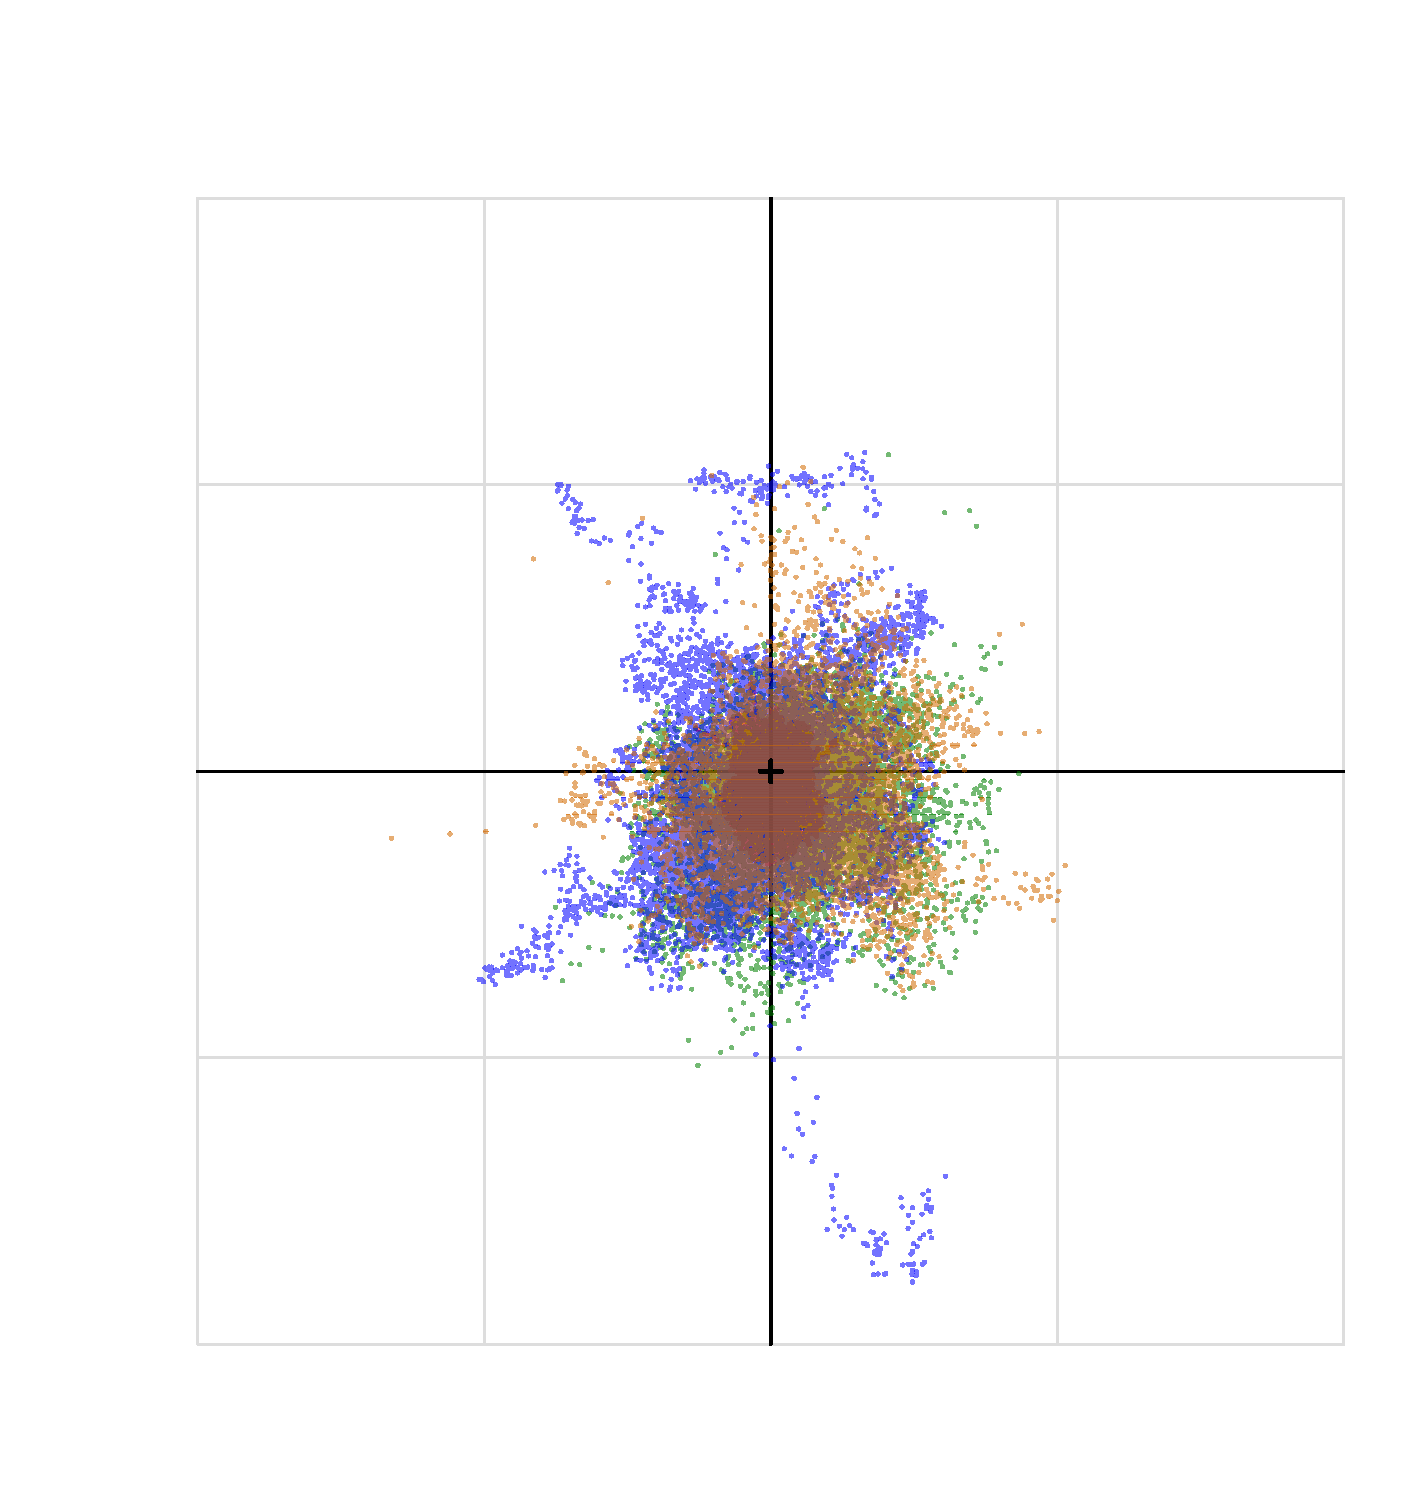
\includegraphics[width=680.0bp,height=715.0bp]{figures/horizontal_detail_en.pdf}}
\put(95.0,692.0){\makebox(0,0)[lb]{\color{black}\sffamily\fontsize{16}{16}\selectfont Detail ±0.10 m (larger errors hidden)}}
\put(95.0,50.0){\makebox(0,0)[cb]{\color{black}\sffamily\fontsize{12}{12}\selectfont -0.1}}
\put(232.5,50.0){\makebox(0,0)[cb]{\color{black}\sffamily\fontsize{12}{12}\selectfont -0.05}}
\put(370.0,50.0){\makebox(0,0)[cb]{\color{black}\sffamily\fontsize{12}{12}\selectfont 0}}
\put(507.50000000000006,50.0){\makebox(0,0)[cb]{\color{black}\sffamily\fontsize{12}{12}\selectfont 0.05}}
\put(645.0,50.0){\makebox(0,0)[cb]{\color{black}\sffamily\fontsize{12}{12}\selectfont 0.1}}
\put(87.0,66.0){\makebox(0,0)[rb]{\color{black}\sffamily\fontsize{12}{12}\selectfont -0.1}}
\put(87.0,203.5){\makebox(0,0)[rb]{\color{black}\sffamily\fontsize{12}{12}\selectfont -0.05}}
\put(87.0,341.0){\makebox(0,0)[rb]{\color{black}\sffamily\fontsize{12}{12}\selectfont 0}}
\put(87.0,478.50000000000006){\makebox(0,0)[rb]{\color{black}\sffamily\fontsize{12}{12}\selectfont 0.05}}
\put(87.0,616.0){\makebox(0,0)[rb]{\color{black}\sffamily\fontsize{12}{12}\selectfont 0.1}}
\put(95.0,670.0){\makebox(0,0)[lb]{\color{red}\sffamily\fontsize{12}{12}\selectfont P23M\_0}}
\put(370.0,670.0){\makebox(0,0)[lb]{\color{green}\sffamily\fontsize{12}{12}\selectfont P23M\_1}}
\put(95.0,648.0){\makebox(0,0)[lb]{\color{blue}\sffamily\fontsize{12}{12}\selectfont UM980}}
\put(370.0,648.0){\makebox(0,0)[lb]{\color[HTML]{d26900}\sffamily\fontsize{12}{12}\selectfont LG290P}}
\put(378.0,353.0){\makebox(0,0)[lb]{\color{black}\sffamily\fontsize{12}{12}\selectfont Expected (0,0)}}
\put(370.0,12.0){\makebox(0,0)[cb]{\color{black}\sffamily\fontsize{12}{12}\selectfont East error [m]}}
\put(19.0,345.0){\rotatebox{90}{\makebox(0,0)[b]{\color{black}\sffamily\fontsize{12}{12}\selectfont North error [m]}}}
\end{picture}}
\end{figure}
\begin{figure}[p]\centering
\resizebox{0.98\linewidth}{!}{%
\setlength{\unitlength}{1bp}\begin{picture}(1000.0,430.0)
\put(0,0){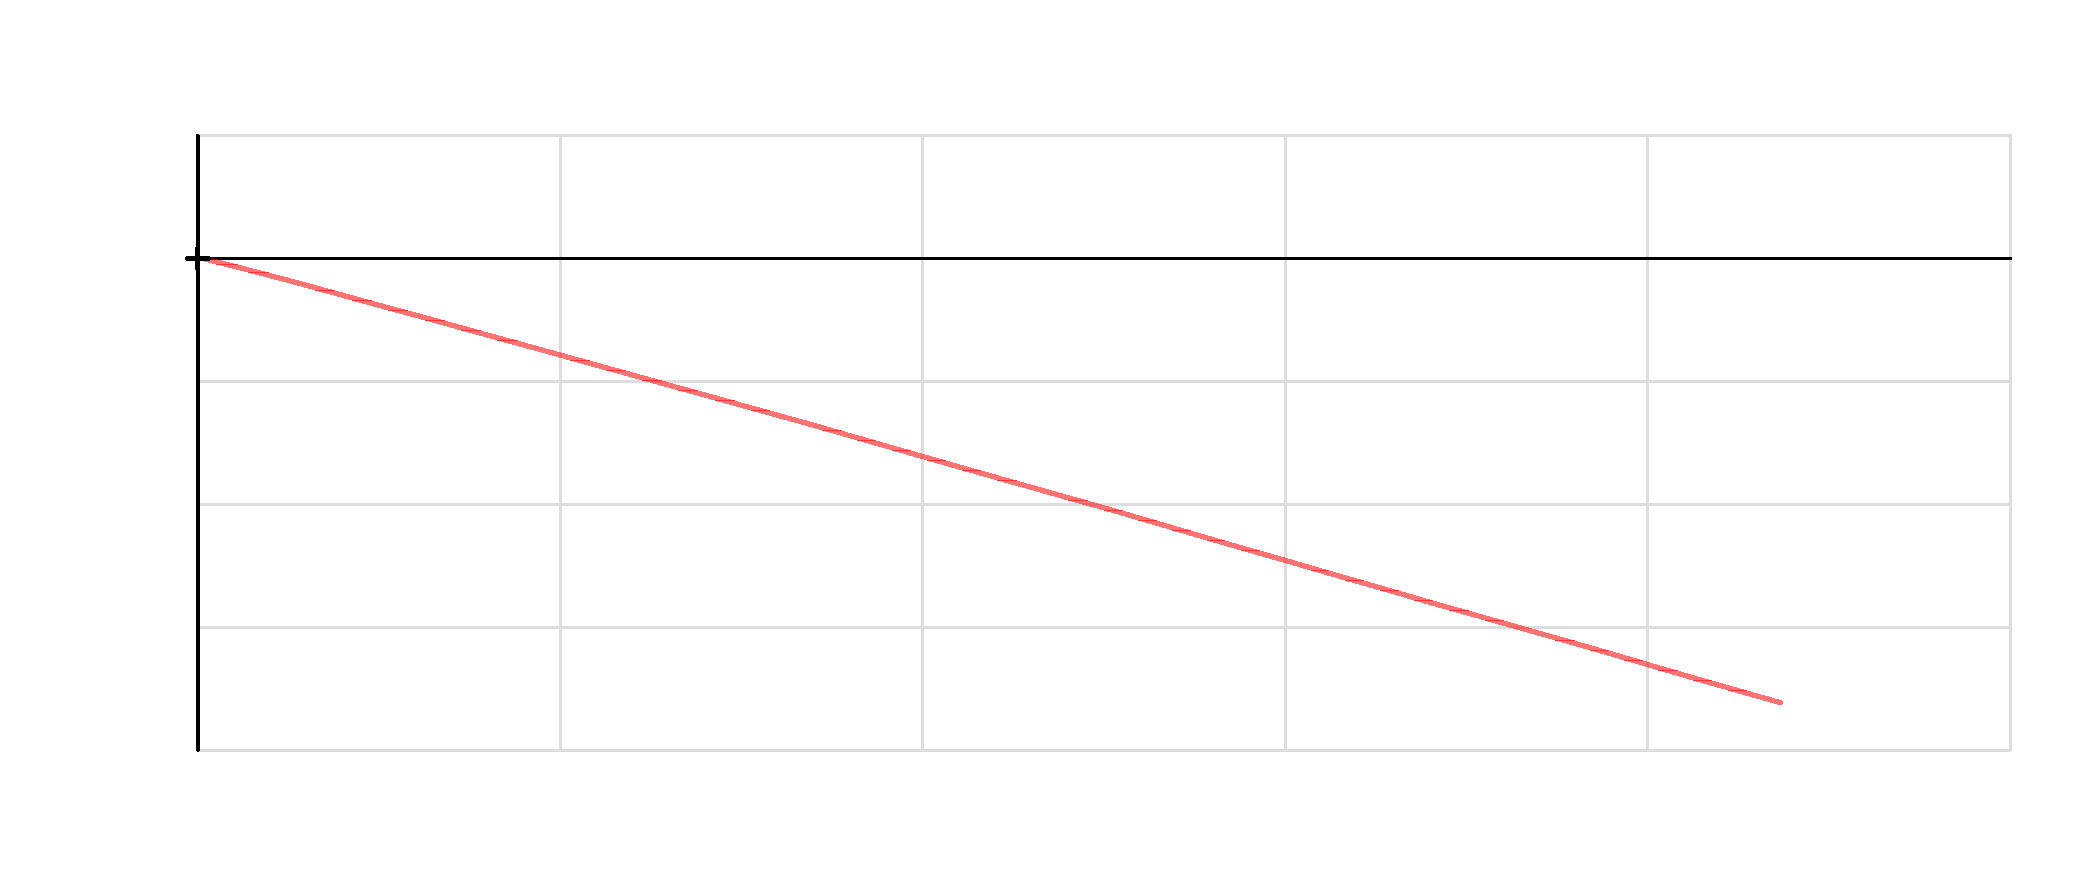
\includegraphics[width=1000.0bp,height=430.0bp]{figures/rotation_en.pdf}}
\put(95.0,407.0){\makebox(0,0)[lb]{\color{black}\sffamily\fontsize{16}{16}\selectfont Revolutions: positive from east towards north}}
\put(95.0,50.0){\makebox(0,0)[cb]{\color{black}\sffamily\fontsize{12}{12}\selectfont 0}}
\put(269.0,50.0){\makebox(0,0)[cb]{\color{black}\sffamily\fontsize{12}{12}\selectfont 50}}
\put(443.0,50.0){\makebox(0,0)[cb]{\color{black}\sffamily\fontsize{12}{12}\selectfont 100}}
\put(617.0,50.0){\makebox(0,0)[cb]{\color{black}\sffamily\fontsize{12}{12}\selectfont 150}}
\put(791.0,50.0){\makebox(0,0)[cb]{\color{black}\sffamily\fontsize{12}{12}\selectfont 200}}
\put(965.0,50.0){\makebox(0,0)[cb]{\color{black}\sffamily\fontsize{12}{12}\selectfont 250}}
\put(87.0,66.0){\makebox(0,0)[rb]{\color{black}\sffamily\fontsize{12}{12}\selectfont -80}}
\put(87.0,125.0){\makebox(0,0)[rb]{\color{black}\sffamily\fontsize{12}{12}\selectfont -60}}
\put(87.0,184.0){\makebox(0,0)[rb]{\color{black}\sffamily\fontsize{12}{12}\selectfont -40}}
\put(87.0,243.0){\makebox(0,0)[rb]{\color{black}\sffamily\fontsize{12}{12}\selectfont -20}}
\put(87.0,302.0){\makebox(0,0)[rb]{\color{black}\sffamily\fontsize{12}{12}\selectfont 0}}
\put(87.0,361.0){\makebox(0,0)[rb]{\color{black}\sffamily\fontsize{12}{12}\selectfont 20}}
\put(95.0,385.0){\makebox(0,0)[lb]{\color{red}\sffamily\fontsize{12}{12}\selectfont P23M\_0}}
\put(103.0,314.0){\makebox(0,0)[lb]{\color{black}\sffamily\fontsize{12}{12}\selectfont (0,0)}}
\put(530.0,12.0){\makebox(0,0)[cb]{\color{black}\sffamily\fontsize{12}{12}\selectfont Time since common start [min]}}
\put(19.0,217.5){\rotatebox{90}{\makebox(0,0)[b]{\color{black}\sffamily\fontsize{12}{12}\selectfont Revolutions since first reference point}}}
\end{picture}}
\end{figure}
\begin{figure}[p]\centering
\resizebox{0.98\linewidth}{!}{%
\setlength{\unitlength}{1bp}\begin{picture}(1000.0,435.0)
\put(0,0){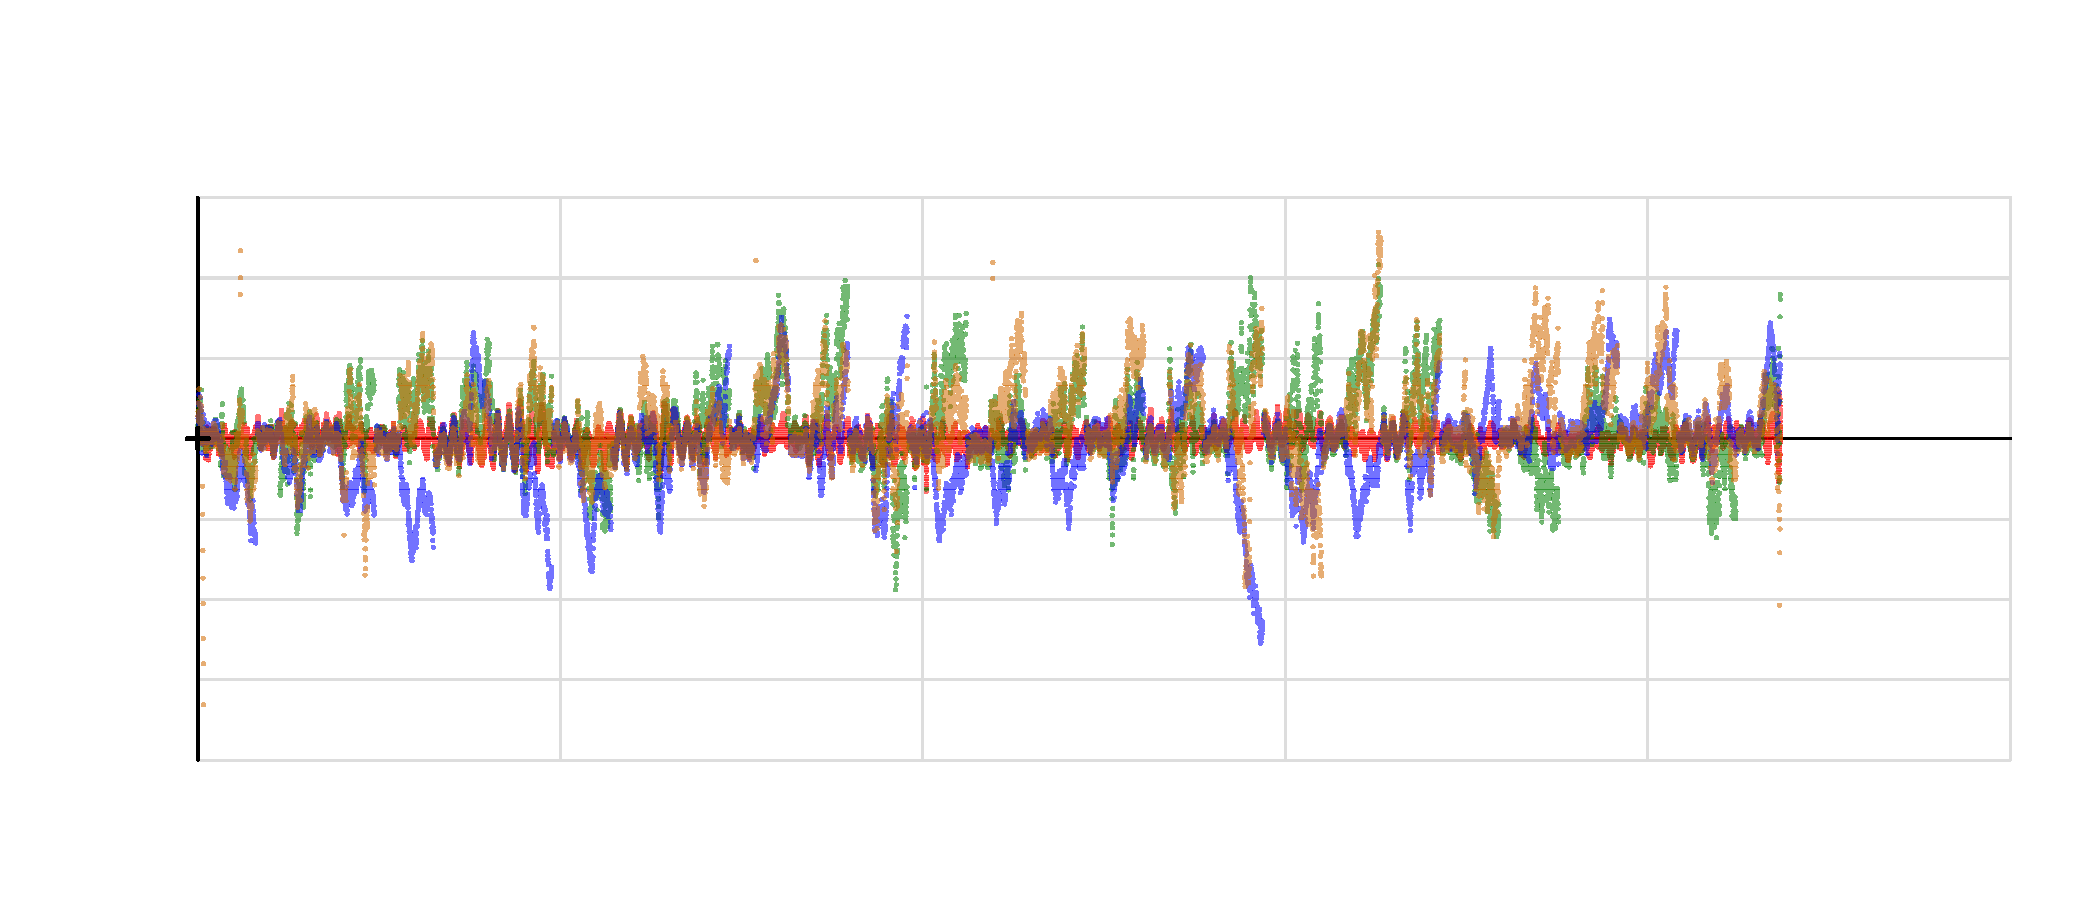
\includegraphics[width=1000.0bp,height=435.0bp]{figures/east_time_en.pdf}}
\put(95.0,412.0){\makebox(0,0)[lb]{\color{black}\sffamily\fontsize{16}{16}\selectfont East error over time}}
\put(95.0,50.0){\makebox(0,0)[cb]{\color{black}\sffamily\fontsize{12}{12}\selectfont 0}}
\put(269.0,50.0){\makebox(0,0)[cb]{\color{black}\sffamily\fontsize{12}{12}\selectfont 50}}
\put(443.0,50.0){\makebox(0,0)[cb]{\color{black}\sffamily\fontsize{12}{12}\selectfont 100}}
\put(617.0,50.0){\makebox(0,0)[cb]{\color{black}\sffamily\fontsize{12}{12}\selectfont 150}}
\put(791.0,50.0){\makebox(0,0)[cb]{\color{black}\sffamily\fontsize{12}{12}\selectfont 200}}
\put(965.0,50.0){\makebox(0,0)[cb]{\color{black}\sffamily\fontsize{12}{12}\selectfont 250}}
\put(87.0,66.0){\makebox(0,0)[rb]{\color{black}\sffamily\fontsize{12}{12}\selectfont -0.08}}
\put(87.0,104.57142857142856){\makebox(0,0)[rb]{\color{black}\sffamily\fontsize{12}{12}\selectfont -0.06}}
\put(87.0,143.1428571428571){\makebox(0,0)[rb]{\color{black}\sffamily\fontsize{12}{12}\selectfont -0.04}}
\put(87.0,181.7142857142857){\makebox(0,0)[rb]{\color{black}\sffamily\fontsize{12}{12}\selectfont -0.02}}
\put(87.0,220.28571428571428){\makebox(0,0)[rb]{\color{black}\sffamily\fontsize{12}{12}\selectfont 0}}
\put(87.0,258.8571428571429){\makebox(0,0)[rb]{\color{black}\sffamily\fontsize{12}{12}\selectfont 0.02}}
\put(87.0,297.4285714285714){\makebox(0,0)[rb]{\color{black}\sffamily\fontsize{12}{12}\selectfont 0.04}}
\put(87.0,336.0){\makebox(0,0)[rb]{\color{black}\sffamily\fontsize{12}{12}\selectfont 0.06}}
\put(95.0,390.0){\makebox(0,0)[lb]{\color{red}\sffamily\fontsize{12}{12}\selectfont P23M\_0}}
\put(530.0,390.0){\makebox(0,0)[lb]{\color{green}\sffamily\fontsize{12}{12}\selectfont P23M\_1}}
\put(95.0,368.0){\makebox(0,0)[lb]{\color{blue}\sffamily\fontsize{12}{12}\selectfont UM980}}
\put(530.0,368.0){\makebox(0,0)[lb]{\color[HTML]{d26900}\sffamily\fontsize{12}{12}\selectfont LG290P}}
\put(103.0,232.28571428571428){\makebox(0,0)[lb]{\color{black}\sffamily\fontsize{12}{12}\selectfont (0,0)}}
\put(530.0,12.0){\makebox(0,0)[cb]{\color{black}\sffamily\fontsize{12}{12}\selectfont Time since common start [min]}}
\put(19.0,205.0){\rotatebox{90}{\makebox(0,0)[b]{\color{black}\sffamily\fontsize{12}{12}\selectfont East error [m]}}}
\end{picture}}
\end{figure}
\begin{figure}[p]\centering
\resizebox{0.98\linewidth}{!}{%
\setlength{\unitlength}{1bp}\begin{picture}(1000.0,435.0)
\put(0,0){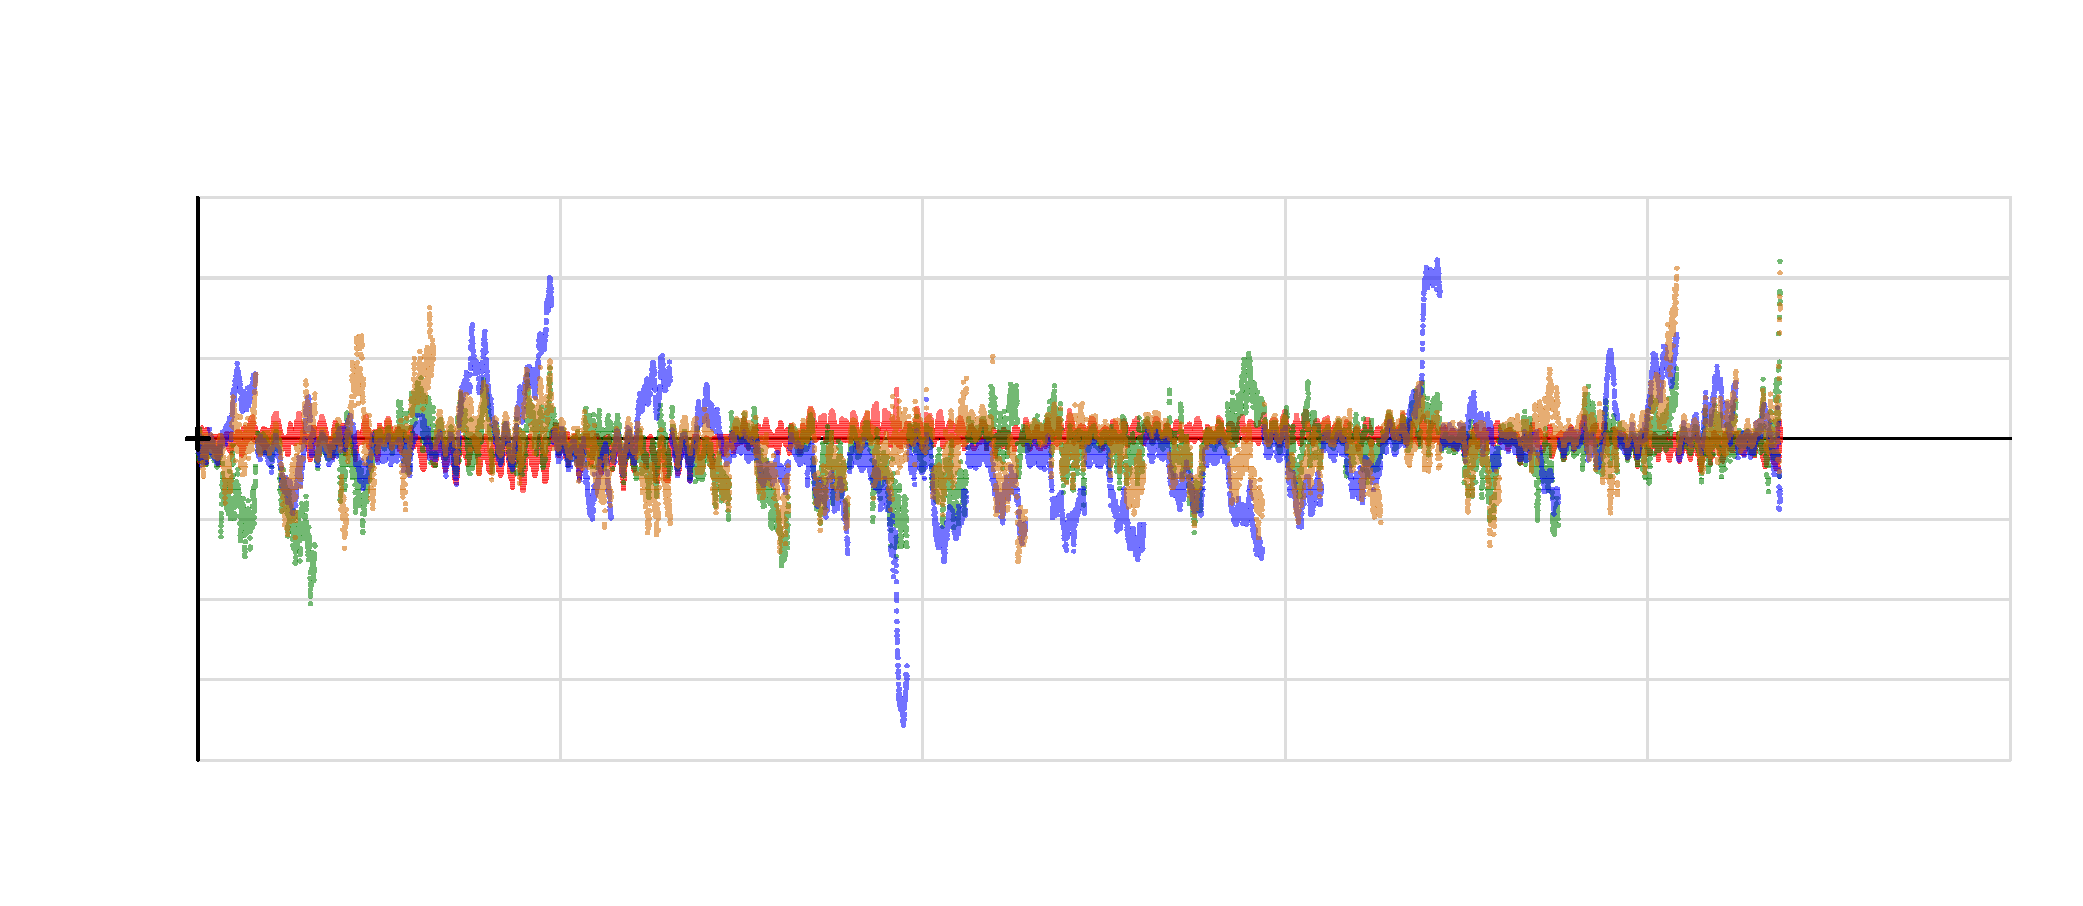
\includegraphics[width=1000.0bp,height=435.0bp]{figures/north_time_en.pdf}}
\put(95.0,412.0){\makebox(0,0)[lb]{\color{black}\sffamily\fontsize{16}{16}\selectfont North error over time}}
\put(95.0,50.0){\makebox(0,0)[cb]{\color{black}\sffamily\fontsize{12}{12}\selectfont 0}}
\put(269.0,50.0){\makebox(0,0)[cb]{\color{black}\sffamily\fontsize{12}{12}\selectfont 50}}
\put(443.0,50.0){\makebox(0,0)[cb]{\color{black}\sffamily\fontsize{12}{12}\selectfont 100}}
\put(617.0,50.0){\makebox(0,0)[cb]{\color{black}\sffamily\fontsize{12}{12}\selectfont 150}}
\put(791.0,50.0){\makebox(0,0)[cb]{\color{black}\sffamily\fontsize{12}{12}\selectfont 200}}
\put(965.0,50.0){\makebox(0,0)[cb]{\color{black}\sffamily\fontsize{12}{12}\selectfont 250}}
\put(87.0,66.0){\makebox(0,0)[rb]{\color{black}\sffamily\fontsize{12}{12}\selectfont -0.1}}
\put(87.0,104.57142857142856){\makebox(0,0)[rb]{\color{black}\sffamily\fontsize{12}{12}\selectfont -0.075}}
\put(87.0,143.1428571428571){\makebox(0,0)[rb]{\color{black}\sffamily\fontsize{12}{12}\selectfont -0.05}}
\put(87.0,181.71428571428572){\makebox(0,0)[rb]{\color{black}\sffamily\fontsize{12}{12}\selectfont -0.025}}
\put(87.0,220.28571428571428){\makebox(0,0)[rb]{\color{black}\sffamily\fontsize{12}{12}\selectfont 0}}
\put(87.0,258.85714285714283){\makebox(0,0)[rb]{\color{black}\sffamily\fontsize{12}{12}\selectfont 0.025}}
\put(87.0,297.42857142857144){\makebox(0,0)[rb]{\color{black}\sffamily\fontsize{12}{12}\selectfont 0.05}}
\put(87.0,336.0){\makebox(0,0)[rb]{\color{black}\sffamily\fontsize{12}{12}\selectfont 0.075}}
\put(95.0,390.0){\makebox(0,0)[lb]{\color{red}\sffamily\fontsize{12}{12}\selectfont P23M\_0}}
\put(530.0,390.0){\makebox(0,0)[lb]{\color{green}\sffamily\fontsize{12}{12}\selectfont P23M\_1}}
\put(95.0,368.0){\makebox(0,0)[lb]{\color{blue}\sffamily\fontsize{12}{12}\selectfont UM980}}
\put(530.0,368.0){\makebox(0,0)[lb]{\color[HTML]{d26900}\sffamily\fontsize{12}{12}\selectfont LG290P}}
\put(103.0,232.28571428571428){\makebox(0,0)[lb]{\color{black}\sffamily\fontsize{12}{12}\selectfont (0,0)}}
\put(530.0,12.0){\makebox(0,0)[cb]{\color{black}\sffamily\fontsize{12}{12}\selectfont Time since common start [min]}}
\put(19.0,205.0){\rotatebox{90}{\makebox(0,0)[b]{\color{black}\sffamily\fontsize{12}{12}\selectfont North error [m]}}}
\end{picture}}
\end{figure}
\begin{figure}[p]\centering
\resizebox{0.98\linewidth}{!}{%
\setlength{\unitlength}{1bp}\begin{picture}(1000.0,435.0)
\put(0,0){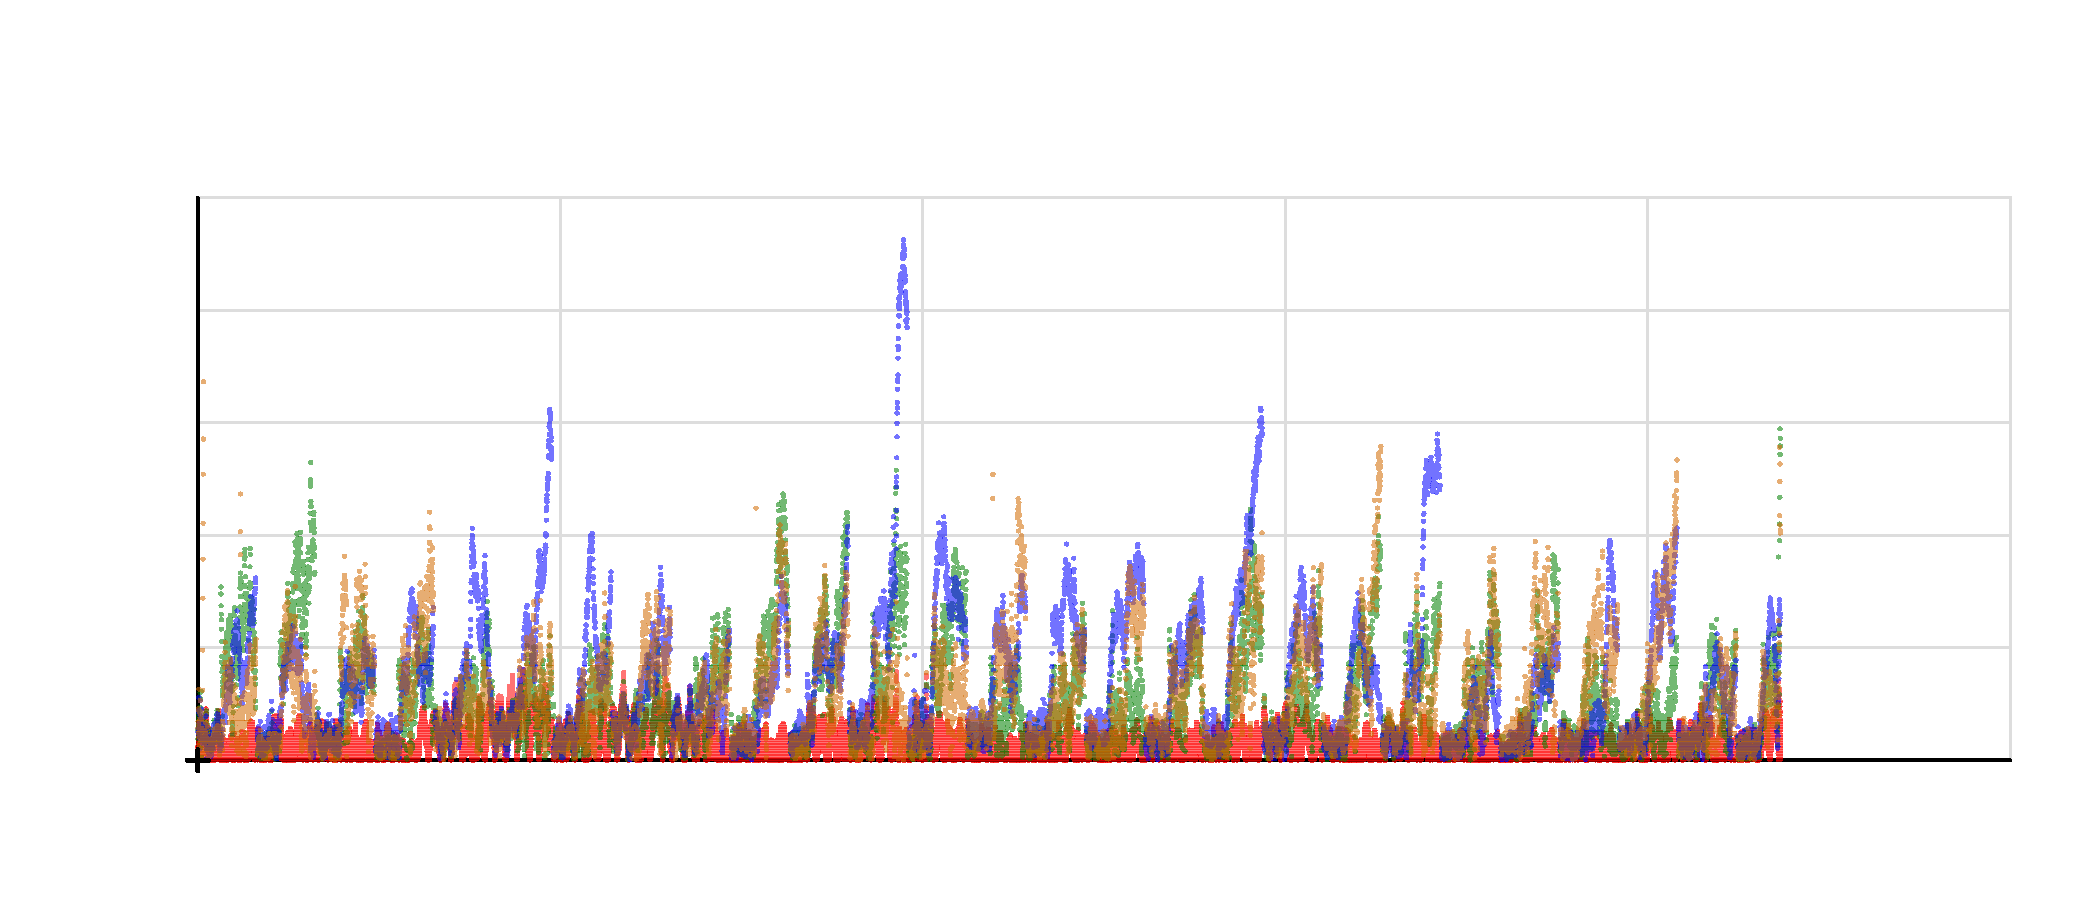
\includegraphics[width=1000.0bp,height=435.0bp]{figures/horizontal_time_en.pdf}}
\put(95.0,412.0){\makebox(0,0)[lb]{\color{black}\sffamily\fontsize{16}{16}\selectfont Horizontal error over time}}
\put(95.0,50.0){\makebox(0,0)[cb]{\color{black}\sffamily\fontsize{12}{12}\selectfont 0}}
\put(269.0,50.0){\makebox(0,0)[cb]{\color{black}\sffamily\fontsize{12}{12}\selectfont 50}}
\put(443.0,50.0){\makebox(0,0)[cb]{\color{black}\sffamily\fontsize{12}{12}\selectfont 100}}
\put(617.0,50.0){\makebox(0,0)[cb]{\color{black}\sffamily\fontsize{12}{12}\selectfont 150}}
\put(791.0,50.0){\makebox(0,0)[cb]{\color{black}\sffamily\fontsize{12}{12}\selectfont 200}}
\put(965.0,50.0){\makebox(0,0)[cb]{\color{black}\sffamily\fontsize{12}{12}\selectfont 250}}
\put(87.0,66.0){\makebox(0,0)[rb]{\color{black}\sffamily\fontsize{12}{12}\selectfont 0}}
\put(87.0,120.0){\makebox(0,0)[rb]{\color{black}\sffamily\fontsize{12}{12}\selectfont 0.02}}
\put(87.0,174.0){\makebox(0,0)[rb]{\color{black}\sffamily\fontsize{12}{12}\selectfont 0.04}}
\put(87.0,228.0){\makebox(0,0)[rb]{\color{black}\sffamily\fontsize{12}{12}\selectfont 0.06}}
\put(87.0,282.0){\makebox(0,0)[rb]{\color{black}\sffamily\fontsize{12}{12}\selectfont 0.08}}
\put(87.0,336.0){\makebox(0,0)[rb]{\color{black}\sffamily\fontsize{12}{12}\selectfont 0.1}}
\put(95.0,390.0){\makebox(0,0)[lb]{\color{red}\sffamily\fontsize{12}{12}\selectfont P23M\_0}}
\put(530.0,390.0){\makebox(0,0)[lb]{\color{green}\sffamily\fontsize{12}{12}\selectfont P23M\_1}}
\put(95.0,368.0){\makebox(0,0)[lb]{\color{blue}\sffamily\fontsize{12}{12}\selectfont UM980}}
\put(530.0,368.0){\makebox(0,0)[lb]{\color[HTML]{d26900}\sffamily\fontsize{12}{12}\selectfont LG290P}}
\put(103.0,78.0){\makebox(0,0)[lb]{\color{black}\sffamily\fontsize{12}{12}\selectfont (0,0)}}
\put(530.0,12.0){\makebox(0,0)[cb]{\color{black}\sffamily\fontsize{12}{12}\selectfont Time since common start [min]}}
\put(19.0,205.0){\rotatebox{90}{\makebox(0,0)[b]{\color{black}\sffamily\fontsize{12}{12}\selectfont Horizontal error [m]}}}
\end{picture}}
\end{figure}
\begin{figure}[p]\centering
\resizebox{0.98\linewidth}{!}{%
\setlength{\unitlength}{1bp}\begin{picture}(1000.0,435.0)
\put(0,0){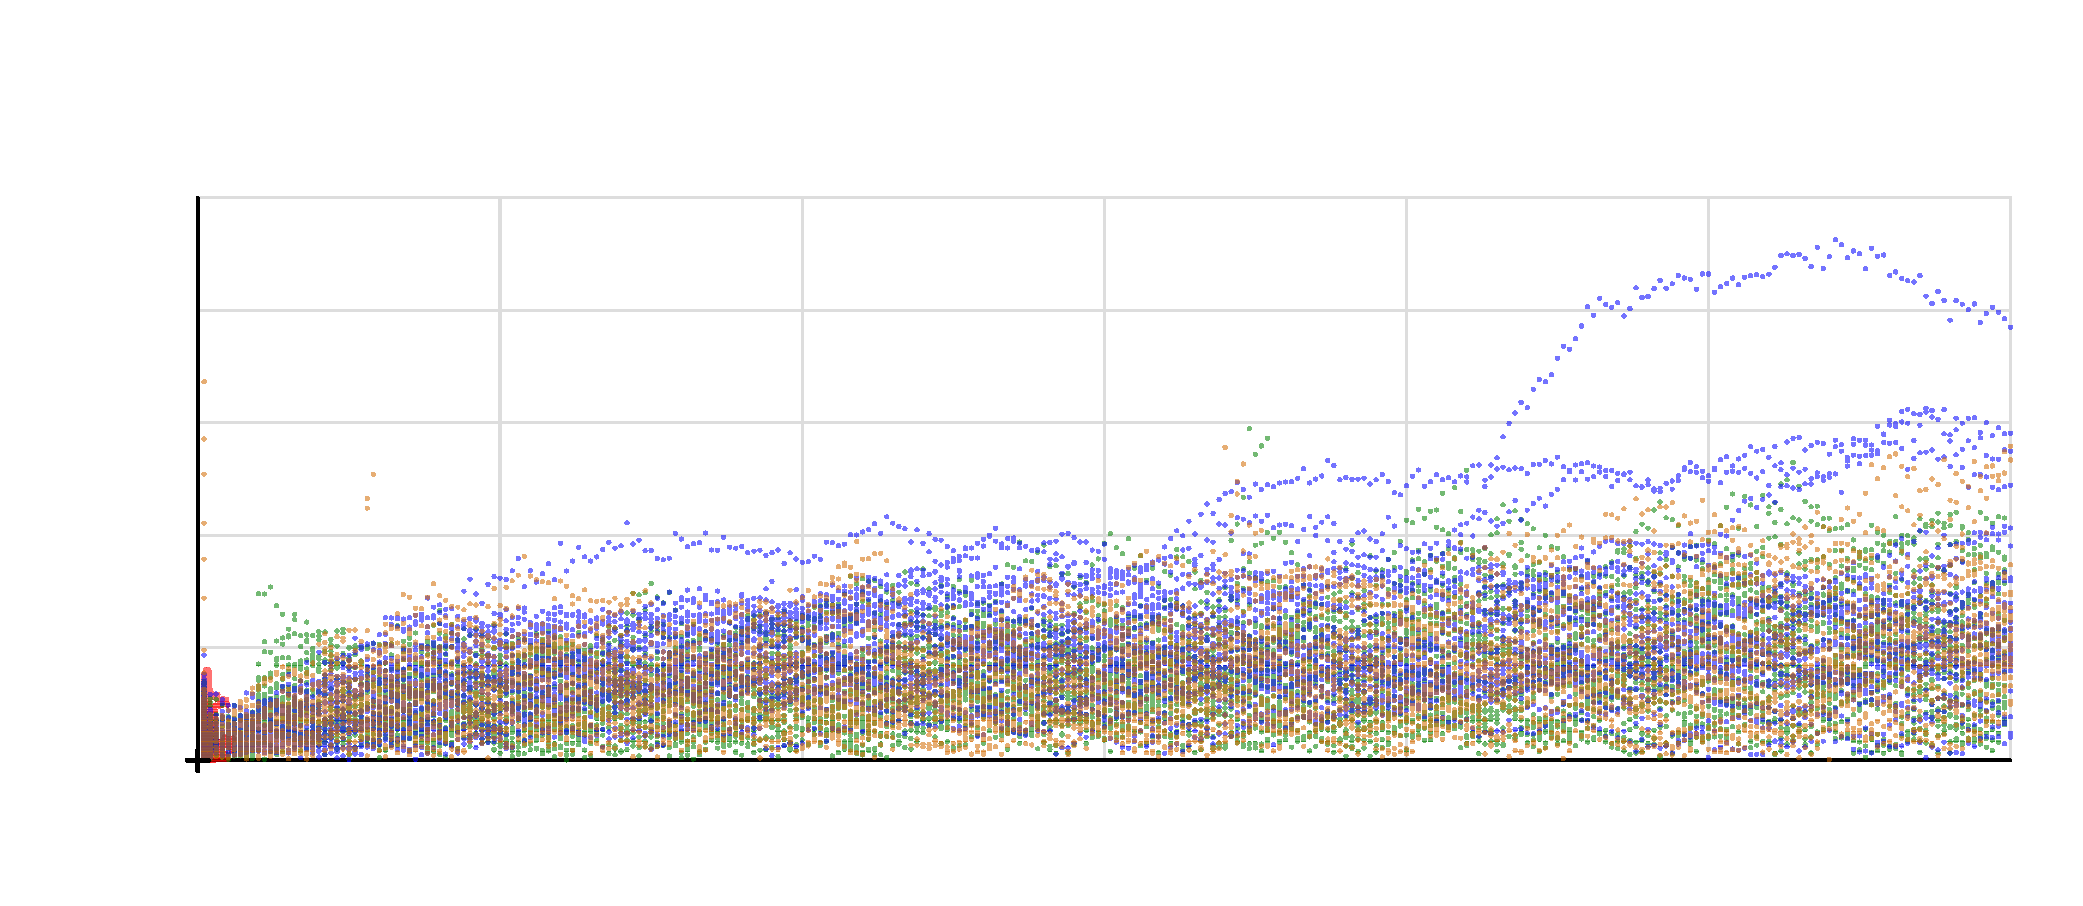
\includegraphics[width=1000.0bp,height=435.0bp]{figures/horizontal_dage_scatter_en.pdf}}
\put(95.0,412.0){\makebox(0,0)[lb]{\color{black}\sffamily\fontsize{16}{16}\selectfont Horizontal error versus dAge: all RTK-fixed samples}}
\put(95.0,50.0){\makebox(0,0)[cb]{\color{black}\sffamily\fontsize{12}{12}\selectfont 0}}
\put(240.0,50.0){\makebox(0,0)[cb]{\color{black}\sffamily\fontsize{12}{12}\selectfont 50}}
\put(385.0,50.0){\makebox(0,0)[cb]{\color{black}\sffamily\fontsize{12}{12}\selectfont 100}}
\put(530.0,50.0){\makebox(0,0)[cb]{\color{black}\sffamily\fontsize{12}{12}\selectfont 150}}
\put(675.0,50.0){\makebox(0,0)[cb]{\color{black}\sffamily\fontsize{12}{12}\selectfont 200}}
\put(820.0,50.0){\makebox(0,0)[cb]{\color{black}\sffamily\fontsize{12}{12}\selectfont 250}}
\put(965.0,50.0){\makebox(0,0)[cb]{\color{black}\sffamily\fontsize{12}{12}\selectfont 300}}
\put(87.0,66.0){\makebox(0,0)[rb]{\color{black}\sffamily\fontsize{12}{12}\selectfont 0}}
\put(87.0,120.0){\makebox(0,0)[rb]{\color{black}\sffamily\fontsize{12}{12}\selectfont 20}}
\put(87.0,174.0){\makebox(0,0)[rb]{\color{black}\sffamily\fontsize{12}{12}\selectfont 40}}
\put(87.0,228.0){\makebox(0,0)[rb]{\color{black}\sffamily\fontsize{12}{12}\selectfont 60}}
\put(87.0,282.0){\makebox(0,0)[rb]{\color{black}\sffamily\fontsize{12}{12}\selectfont 80}}
\put(87.0,336.0){\makebox(0,0)[rb]{\color{black}\sffamily\fontsize{12}{12}\selectfont 100}}
\put(95.0,390.0){\makebox(0,0)[lb]{\color{red}\sffamily\fontsize{12}{12}\selectfont P23M\_0}}
\put(530.0,390.0){\makebox(0,0)[lb]{\color{green}\sffamily\fontsize{12}{12}\selectfont P23M\_1}}
\put(95.0,368.0){\makebox(0,0)[lb]{\color{blue}\sffamily\fontsize{12}{12}\selectfont UM980}}
\put(530.0,368.0){\makebox(0,0)[lb]{\color[HTML]{d26900}\sffamily\fontsize{12}{12}\selectfont LG290P}}
\put(103.0,78.0){\makebox(0,0)[lb]{\color{black}\sffamily\fontsize{12}{12}\selectfont (0,0)}}
\put(530.0,12.0){\makebox(0,0)[cb]{\color{black}\sffamily\fontsize{12}{12}\selectfont Correction age dAge [s]}}
\put(19.0,205.0){\rotatebox{90}{\makebox(0,0)[b]{\color{black}\sffamily\fontsize{12}{12}\selectfont Horizontal error [mm]}}}
\end{picture}}
\end{figure}
\begin{figure}[p]\centering
\resizebox{0.98\linewidth}{!}{%
\setlength{\unitlength}{1bp}\begin{picture}(1000.0,479.0)
\put(0,0){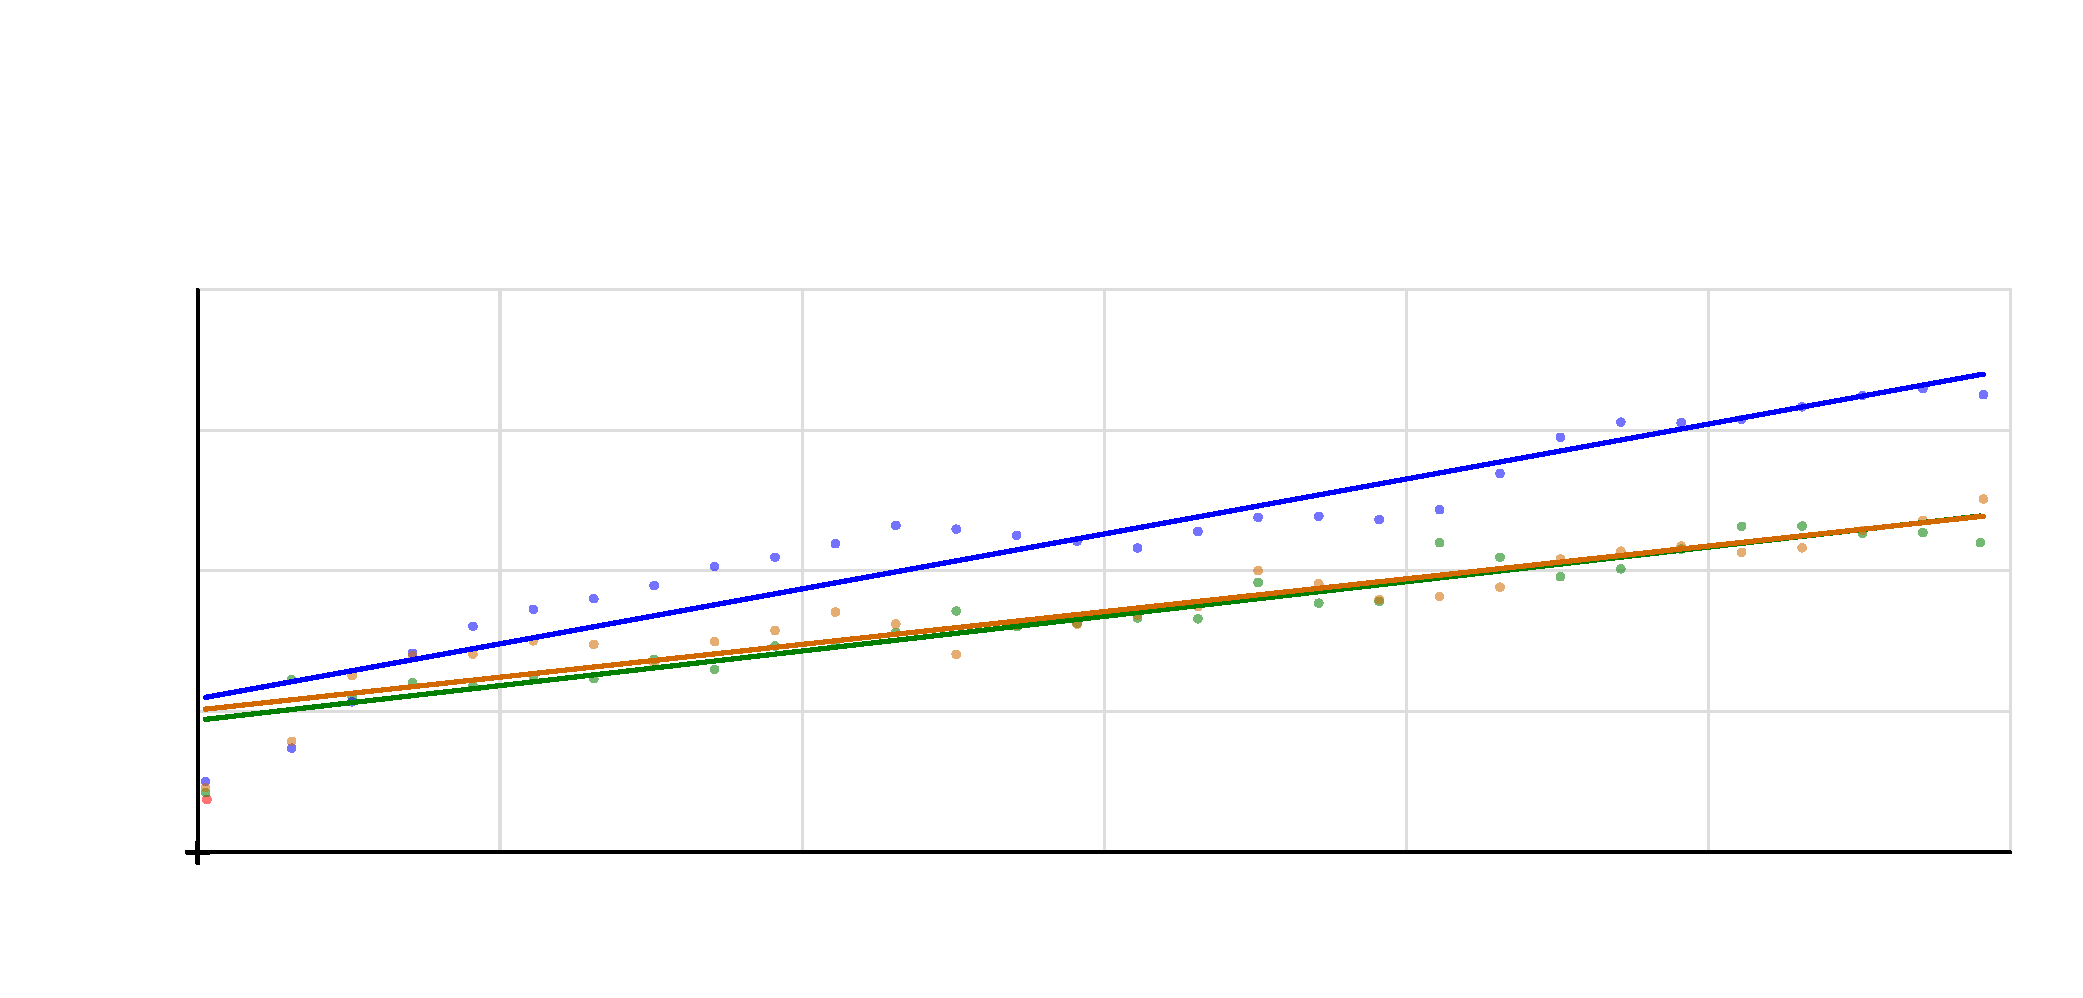
\includegraphics[width=1000.0bp,height=479.0bp]{figures/horizontal_dage_en.pdf}}
\put(95.0,456.0){\makebox(0,0)[lb]{\color{black}\sffamily\fontsize{16}{16}\selectfont HRMS versus dAge: 10-s bins and linear fit}}
\put(95.0,50.0){\makebox(0,0)[cb]{\color{black}\sffamily\fontsize{12}{12}\selectfont 0}}
\put(240.0,50.0){\makebox(0,0)[cb]{\color{black}\sffamily\fontsize{12}{12}\selectfont 50}}
\put(385.0,50.0){\makebox(0,0)[cb]{\color{black}\sffamily\fontsize{12}{12}\selectfont 100}}
\put(530.0,50.0){\makebox(0,0)[cb]{\color{black}\sffamily\fontsize{12}{12}\selectfont 150}}
\put(675.0,50.0){\makebox(0,0)[cb]{\color{black}\sffamily\fontsize{12}{12}\selectfont 200}}
\put(820.0,50.0){\makebox(0,0)[cb]{\color{black}\sffamily\fontsize{12}{12}\selectfont 250}}
\put(965.0,50.0){\makebox(0,0)[cb]{\color{black}\sffamily\fontsize{12}{12}\selectfont 300}}
\put(87.0,66.0){\makebox(0,0)[rb]{\color{black}\sffamily\fontsize{12}{12}\selectfont 0}}
\put(87.0,133.5){\makebox(0,0)[rb]{\color{black}\sffamily\fontsize{12}{12}\selectfont 10}}
\put(87.0,201.0){\makebox(0,0)[rb]{\color{black}\sffamily\fontsize{12}{12}\selectfont 20}}
\put(87.0,268.5){\makebox(0,0)[rb]{\color{black}\sffamily\fontsize{12}{12}\selectfont 30}}
\put(87.0,336.0){\makebox(0,0)[rb]{\color{black}\sffamily\fontsize{12}{12}\selectfont 40}}
\put(95.0,434.0){\makebox(0,0)[lb]{\color{red}\sffamily\fontsize{12}{12}\selectfont P23M\_0}}
\put(530.0,434.0){\makebox(0,0)[lb]{\color{green}\sffamily\fontsize{12}{12}\selectfont P23M\_1}}
\put(95.0,412.0){\makebox(0,0)[lb]{\color{blue}\sffamily\fontsize{12}{12}\selectfont UM980}}
\put(530.0,412.0){\makebox(0,0)[lb]{\color[HTML]{d26900}\sffamily\fontsize{12}{12}\selectfont LG290P}}
\put(95.0,390.0){\makebox(0,0)[lb]{\color{green}\sffamily\fontsize{12}{12}\selectfont P23M\_1: +0.0492 mm/\allowbreak{}s}}
\put(530.0,390.0){\makebox(0,0)[lb]{\color{blue}\sffamily\fontsize{12}{12}\selectfont UM980: +0.0781 mm/\allowbreak{}s}}
\put(95.0,368.0){\makebox(0,0)[lb]{\color[HTML]{d26900}\sffamily\fontsize{12}{12}\selectfont LG290P: +0.0466 mm/\allowbreak{}s}}
\put(103.0,78.0){\makebox(0,0)[lb]{\color{black}\sffamily\fontsize{12}{12}\selectfont (0,0)}}
\put(530.0,12.0){\makebox(0,0)[cb]{\color{black}\sffamily\fontsize{12}{12}\selectfont Correction age dAge [s]}}
\put(19.0,205.0){\rotatebox{90}{\makebox(0,0)[b]{\color{black}\sffamily\fontsize{12}{12}\selectfont Horizontal RMS error HRMS [mm]}}}
\end{picture}}
\end{figure}
\begin{figure}[p]\centering
\resizebox{0.98\linewidth}{!}{%
\setlength{\unitlength}{1bp}\begin{picture}(1000.0,545.0)
\put(0,0){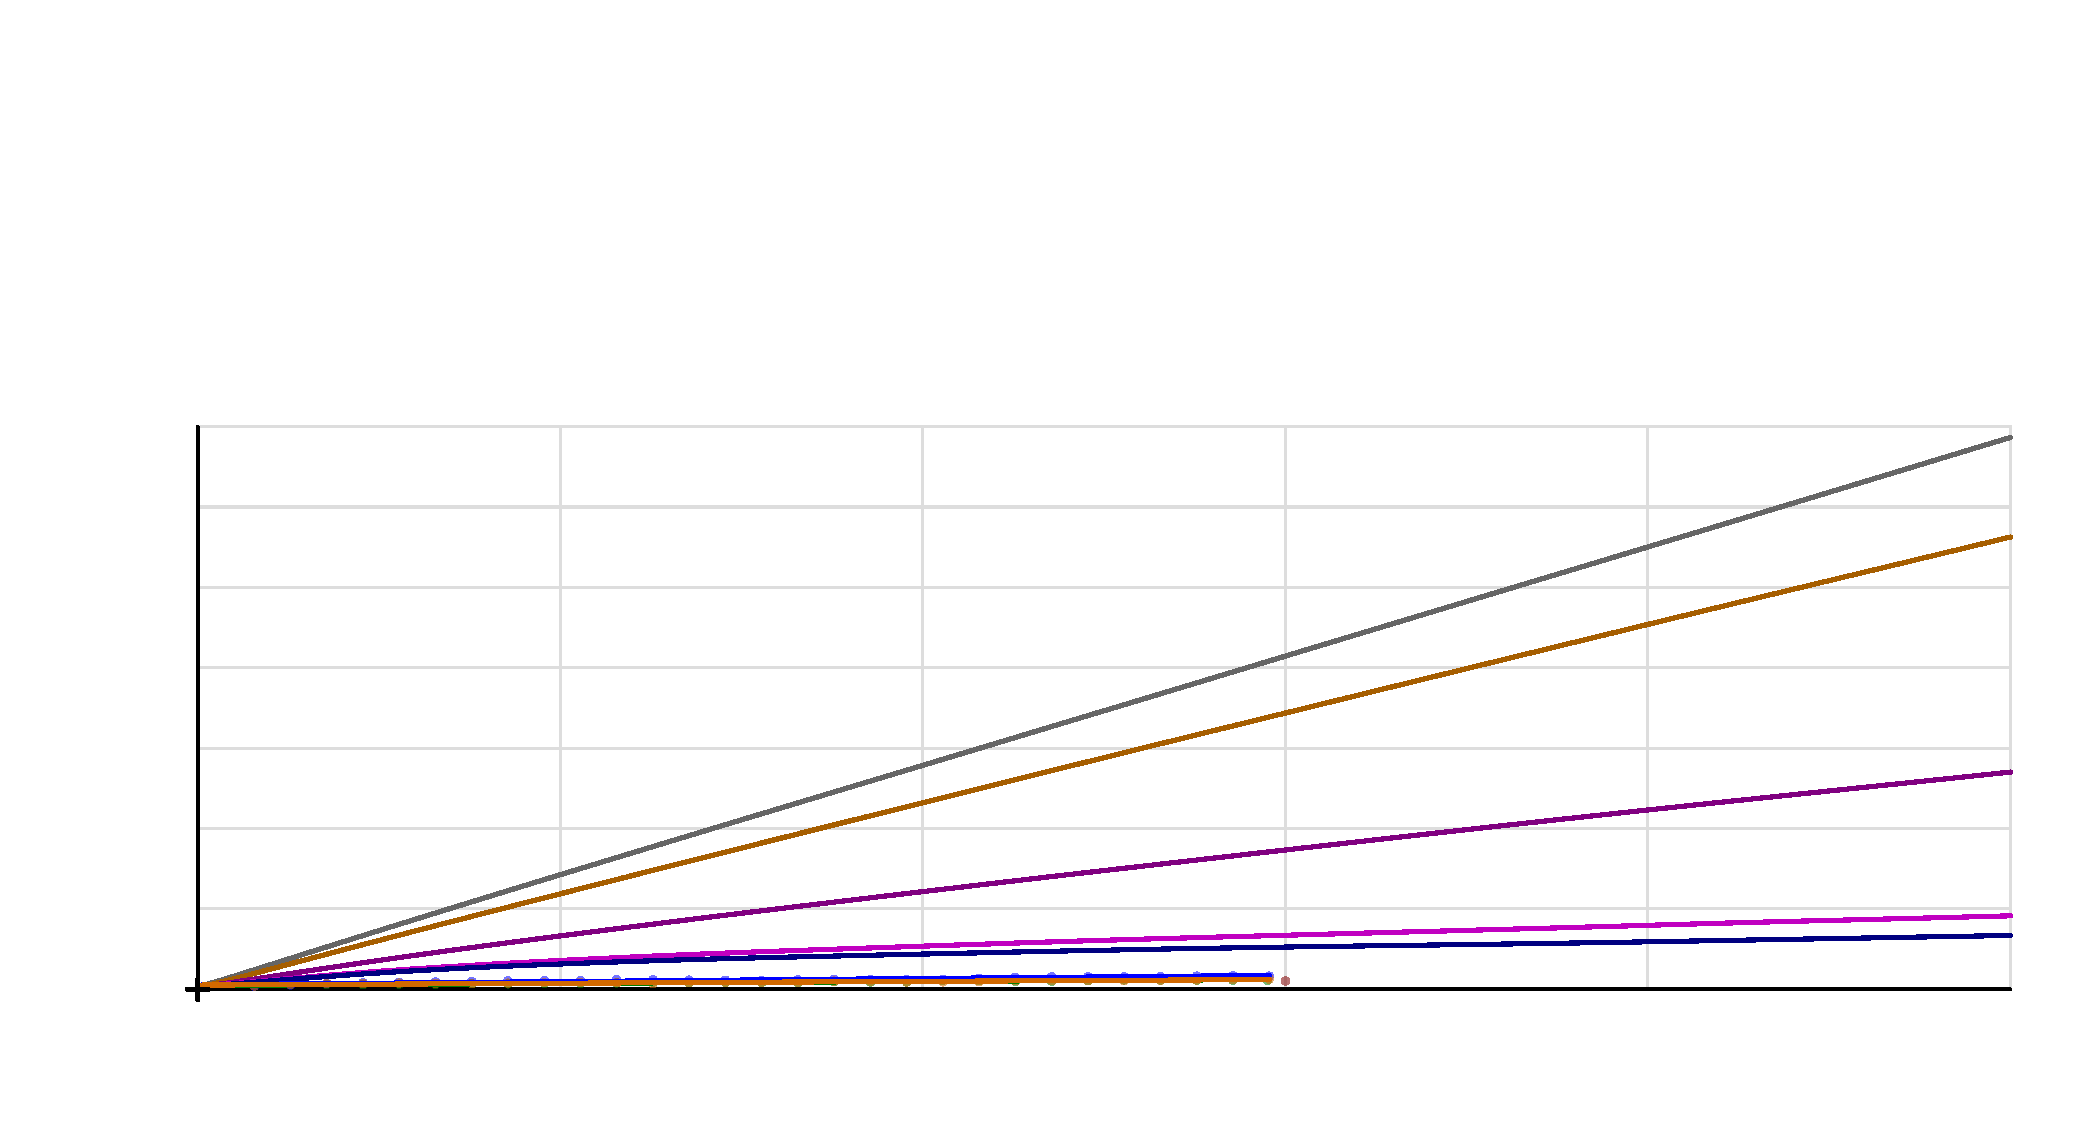
\includegraphics[width=1000.0bp,height=545.0bp]{figures/historical_comparison_en.pdf}}
\put(95.0,522.0){\makebox(0,0)[lb]{\color{black}\sffamily\fontsize{16}{16}\selectfont HRMS(dAge): earlier study and new results}}
\put(95.0,50.0){\makebox(0,0)[cb]{\color{black}\sffamily\fontsize{12}{12}\selectfont 0}}
\put(269.0,50.0){\makebox(0,0)[cb]{\color{black}\sffamily\fontsize{12}{12}\selectfont 100}}
\put(443.0,50.0){\makebox(0,0)[cb]{\color{black}\sffamily\fontsize{12}{12}\selectfont 200}}
\put(617.0,50.0){\makebox(0,0)[cb]{\color{black}\sffamily\fontsize{12}{12}\selectfont 300}}
\put(791.0,50.0){\makebox(0,0)[cb]{\color{black}\sffamily\fontsize{12}{12}\selectfont 400}}
\put(965.0,50.0){\makebox(0,0)[cb]{\color{black}\sffamily\fontsize{12}{12}\selectfont 500}}
\put(87.0,66.0){\makebox(0,0)[rb]{\color{black}\sffamily\fontsize{12}{12}\selectfont 0}}
\put(87.0,104.57142857142856){\makebox(0,0)[rb]{\color{black}\sffamily\fontsize{12}{12}\selectfont 200}}
\put(87.0,143.1428571428571){\makebox(0,0)[rb]{\color{black}\sffamily\fontsize{12}{12}\selectfont 400}}
\put(87.0,181.71428571428572){\makebox(0,0)[rb]{\color{black}\sffamily\fontsize{12}{12}\selectfont 600}}
\put(87.0,220.28571428571428){\makebox(0,0)[rb]{\color{black}\sffamily\fontsize{12}{12}\selectfont 800}}
\put(87.0,258.8571428571429){\makebox(0,0)[rb]{\color{black}\sffamily\fontsize{12}{12}\selectfont 1000}}
\put(87.0,297.42857142857144){\makebox(0,0)[rb]{\color{black}\sffamily\fontsize{12}{12}\selectfont 1200}}
\put(87.0,336.0){\makebox(0,0)[rb]{\color{black}\sffamily\fontsize{12}{12}\selectfont 1400}}
\put(95.0,500.0){\makebox(0,0)[lb]{\color{red}\sffamily\fontsize{12}{12}\selectfont P23M\_0}}
\put(530.0,500.0){\makebox(0,0)[lb]{\color{green}\sffamily\fontsize{12}{12}\selectfont P23M\_1}}
\put(95.0,478.0){\makebox(0,0)[lb]{\color{blue}\sffamily\fontsize{12}{12}\selectfont UM980}}
\put(530.0,478.0){\makebox(0,0)[lb]{\color[HTML]{d26900}\sffamily\fontsize{12}{12}\selectfont LG290P}}
\put(95.0,456.0){\makebox(0,0)[lb]{\color[HTML]{800000}\sffamily\fontsize{12}{12}\selectfont Earlier: precise clocks (one point)}}
\put(95.0,434.0){\makebox(0,0)[lb]{\color[HTML]{666666}\sffamily\fontsize{12}{12}\selectfont Earlier: no SV clock}}
\put(530.0,434.0){\makebox(0,0)[lb]{\color[HTML]{a65e00}\sffamily\fontsize{12}{12}\selectfont Earlier: SV clock}}
\put(95.0,412.0){\makebox(0,0)[lb]{\color[HTML]{800080}\sffamily\fontsize{12}{12}\selectfont Earlier: SV clock + relativity}}
\put(530.0,412.0){\makebox(0,0)[lb]{\color[HTML]{c000c0}\sffamily\fontsize{12}{12}\selectfont Earlier: + ultra-rapid}}
\put(95.0,390.0){\makebox(0,0)[lb]{\color[HTML]{000080}\sffamily\fontsize{12}{12}\selectfont Earlier: + precise orbits}}
\put(530.0,390.0){\makebox(0,0)[lb]{\color{green}\sffamily\fontsize{12}{12}\selectfont P23M\_1: +0.0492 mm/\allowbreak{}s}}
\put(95.0,368.0){\makebox(0,0)[lb]{\color{blue}\sffamily\fontsize{12}{12}\selectfont UM980: +0.0781 mm/\allowbreak{}s}}
\put(530.0,368.0){\makebox(0,0)[lb]{\color[HTML]{d26900}\sffamily\fontsize{12}{12}\selectfont LG290P: +0.0466 mm/\allowbreak{}s}}
\put(103.0,78.0){\makebox(0,0)[lb]{\color{black}\sffamily\fontsize{12}{12}\selectfont (0,0)}}
\put(530.0,12.0){\makebox(0,0)[cb]{\color{black}\sffamily\fontsize{12}{12}\selectfont Correction age dAge [s]}}
\put(19.0,205.0){\rotatebox{90}{\makebox(0,0)[b]{\color{black}\sffamily\fontsize{12}{12}\selectfont Horizontal RMS error HRMS [mm]}}}
\end{picture}}
\end{figure}
\begin{figure}[p]\centering
\resizebox{0.98\linewidth}{!}{%
\setlength{\unitlength}{1bp}\begin{picture}(1000.0,523.0)
\put(0,0){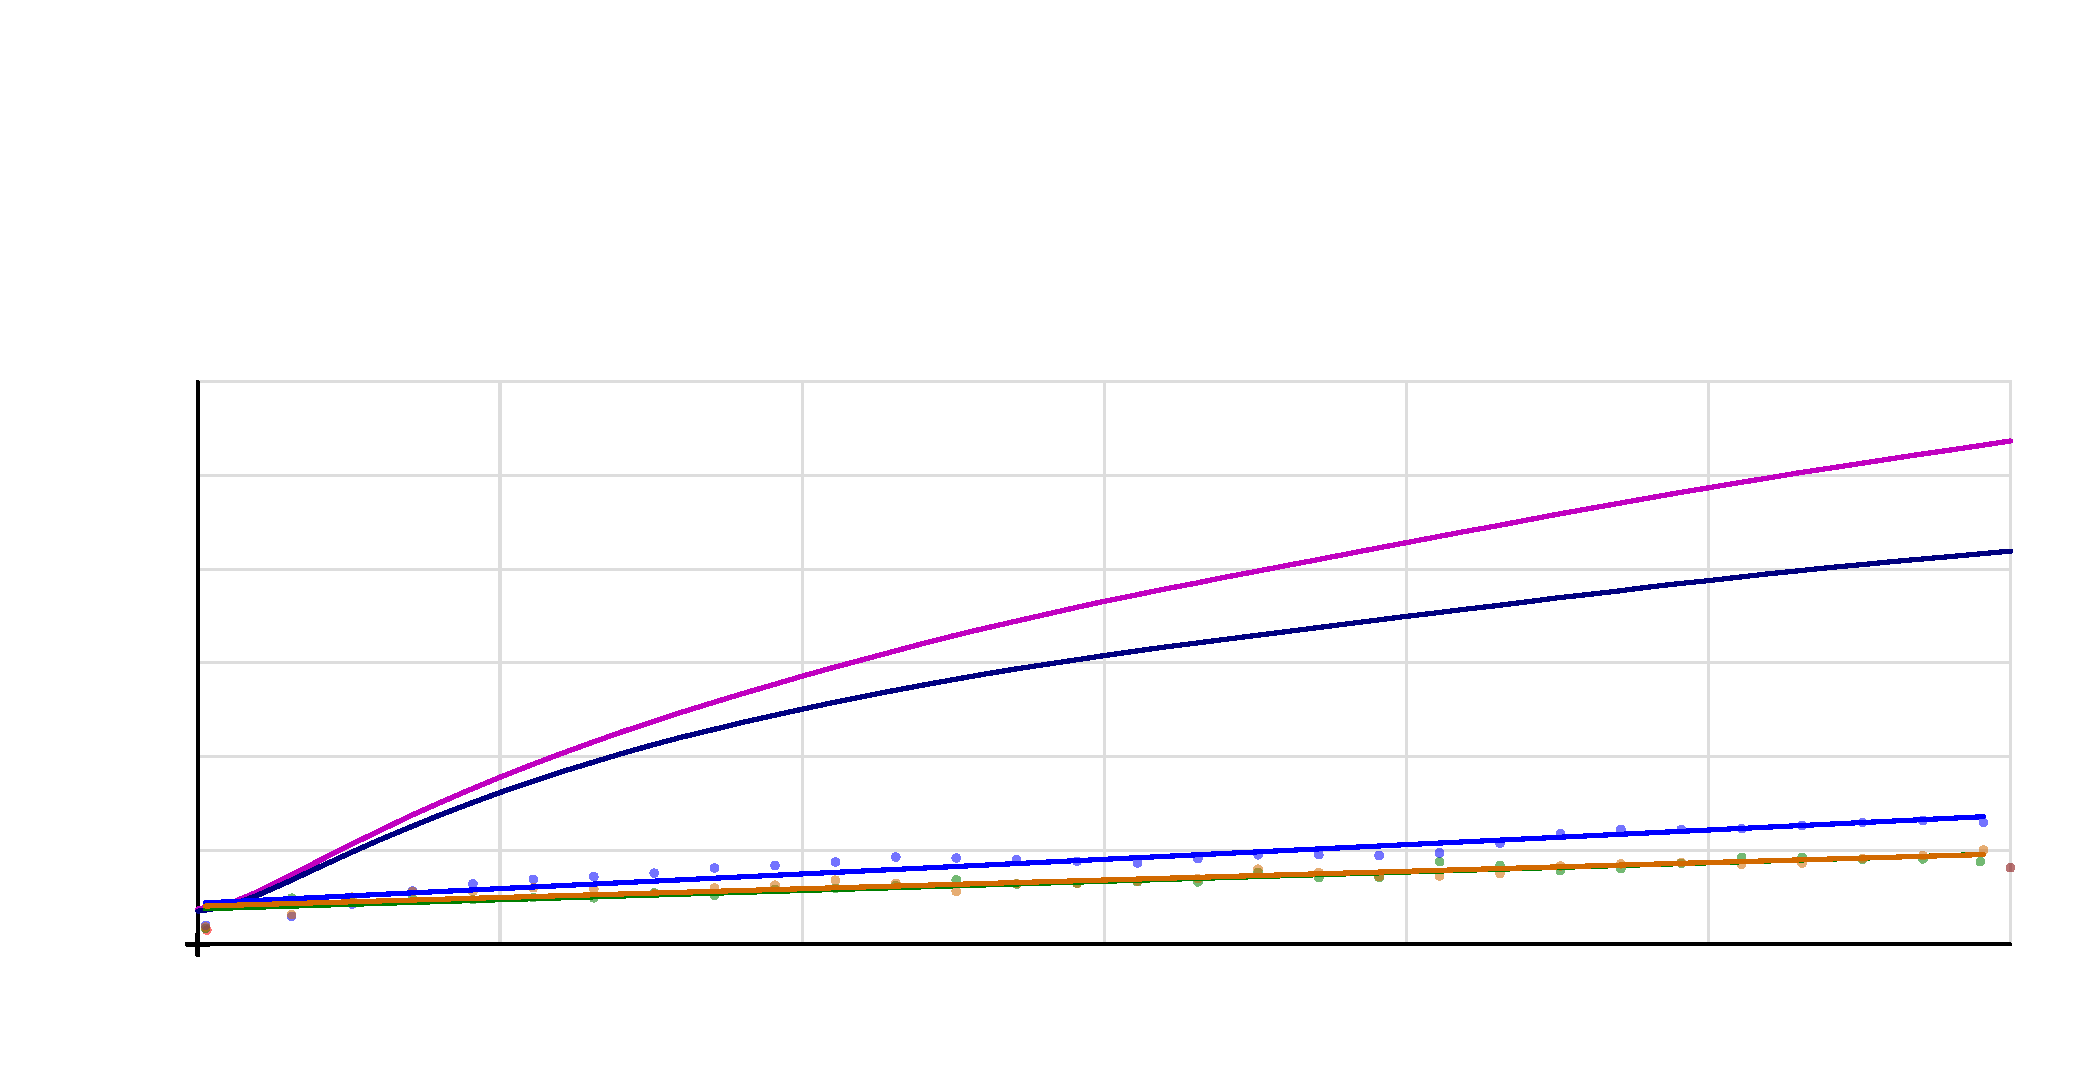
\includegraphics[width=1000.0bp,height=523.0bp]{figures/historical_comparison_detail_en.pdf}}
\put(95.0,500.0){\makebox(0,0)[lb]{\color{black}\sffamily\fontsize{16}{16}\selectfont HRMS(dAge): comparison detail (0–300 s, 0–150 mm)}}
\put(95.0,50.0){\makebox(0,0)[cb]{\color{black}\sffamily\fontsize{12}{12}\selectfont 0}}
\put(240.0,50.0){\makebox(0,0)[cb]{\color{black}\sffamily\fontsize{12}{12}\selectfont 50}}
\put(385.0,50.0){\makebox(0,0)[cb]{\color{black}\sffamily\fontsize{12}{12}\selectfont 100}}
\put(530.0,50.0){\makebox(0,0)[cb]{\color{black}\sffamily\fontsize{12}{12}\selectfont 150}}
\put(675.0,50.0){\makebox(0,0)[cb]{\color{black}\sffamily\fontsize{12}{12}\selectfont 200}}
\put(820.0,50.0){\makebox(0,0)[cb]{\color{black}\sffamily\fontsize{12}{12}\selectfont 250}}
\put(965.0,50.0){\makebox(0,0)[cb]{\color{black}\sffamily\fontsize{12}{12}\selectfont 300}}
\put(87.0,66.0){\makebox(0,0)[rb]{\color{black}\sffamily\fontsize{12}{12}\selectfont 0}}
\put(87.0,111.0){\makebox(0,0)[rb]{\color{black}\sffamily\fontsize{12}{12}\selectfont 25}}
\put(87.0,156.0){\makebox(0,0)[rb]{\color{black}\sffamily\fontsize{12}{12}\selectfont 50}}
\put(87.0,201.0){\makebox(0,0)[rb]{\color{black}\sffamily\fontsize{12}{12}\selectfont 75}}
\put(87.0,246.0){\makebox(0,0)[rb]{\color{black}\sffamily\fontsize{12}{12}\selectfont 100}}
\put(87.0,291.0){\makebox(0,0)[rb]{\color{black}\sffamily\fontsize{12}{12}\selectfont 125}}
\put(87.0,336.0){\makebox(0,0)[rb]{\color{black}\sffamily\fontsize{12}{12}\selectfont 150}}
\put(95.0,478.0){\makebox(0,0)[lb]{\color{red}\sffamily\fontsize{12}{12}\selectfont P23M\_0}}
\put(530.0,478.0){\makebox(0,0)[lb]{\color{green}\sffamily\fontsize{12}{12}\selectfont P23M\_1}}
\put(95.0,456.0){\makebox(0,0)[lb]{\color{blue}\sffamily\fontsize{12}{12}\selectfont UM980}}
\put(530.0,456.0){\makebox(0,0)[lb]{\color[HTML]{d26900}\sffamily\fontsize{12}{12}\selectfont LG290P}}
\put(95.0,434.0){\makebox(0,0)[lb]{\color[HTML]{800000}\sffamily\fontsize{12}{12}\selectfont Earlier: precise clocks (one point)}}
\put(95.0,412.0){\makebox(0,0)[lb]{\color[HTML]{c000c0}\sffamily\fontsize{12}{12}\selectfont Earlier: + ultra-rapid}}
\put(530.0,412.0){\makebox(0,0)[lb]{\color[HTML]{000080}\sffamily\fontsize{12}{12}\selectfont Earlier: + precise orbits}}
\put(95.0,390.0){\makebox(0,0)[lb]{\color{green}\sffamily\fontsize{12}{12}\selectfont P23M\_1: +0.0492 mm/\allowbreak{}s}}
\put(530.0,390.0){\makebox(0,0)[lb]{\color{blue}\sffamily\fontsize{12}{12}\selectfont UM980: +0.0781 mm/\allowbreak{}s}}
\put(95.0,368.0){\makebox(0,0)[lb]{\color[HTML]{d26900}\sffamily\fontsize{12}{12}\selectfont LG290P: +0.0466 mm/\allowbreak{}s}}
\put(103.0,78.0){\makebox(0,0)[lb]{\color{black}\sffamily\fontsize{12}{12}\selectfont (0,0)}}
\put(530.0,12.0){\makebox(0,0)[cb]{\color{black}\sffamily\fontsize{12}{12}\selectfont Correction age dAge [s]}}
\put(19.0,205.0){\rotatebox{90}{\makebox(0,0)[b]{\color{black}\sffamily\fontsize{12}{12}\selectfont Horizontal RMS error HRMS [mm]}}}
\end{picture}}
\end{figure}\clearpage
\clearpage\section{{\cjkfont 中}\allowbreak{}{\cjkfont 文}\allowbreak{}{\cjkfont （}\allowbreak{}{\cjkfont 简}\allowbreak{}{\cjkfont 体}\allowbreak{}{\cjkfont ）}\allowbreak{}— {\cjkfont 转}\allowbreak{}{\cjkfont 台}\allowbreak{}{\cjkfont 测}\allowbreak{}{\cjkfont 试}\allowbreak{} — 2026{\cjkfont 年}\allowbreak{}11{\cjkfont 月}\allowbreak{}7{\cjkfont 日}\allowbreak{}}

\begin{quote}\ttfamily\footnotesize python3 analysis/\allowbreak{}turn\_table.py --dataset datasets/\allowbreak{}2026-11-07\\python3 analysis/\allowbreak{}build\_report.py --dataset datasets/\allowbreak{}2026-11-07\end{quote}

\subsection{{\cjkfont 测}\allowbreak{}{\cjkfont 试}\allowbreak{}{\cjkfont 设}\allowbreak{}{\cjkfont 置}\allowbreak{}{\cjkfont 与}\allowbreak{}{\cjkfont 方}\allowbreak{}{\cjkfont 法}\allowbreak{}}

{\cjkfont 根}\allowbreak{}{\cjkfont 据}\allowbreak{} {\small\texttt{P23M\_\allowbreak{}continious.nmea}} {\cjkfont 文}\allowbreak{}{\cjkfont 件}\allowbreak{}{\cjkfont 名}\allowbreak{}{\cjkfont ，}\allowbreak{}{\cjkfont 将}\allowbreak{} P23M\_0 {\cjkfont 作}\allowbreak{}{\cjkfont 为}\allowbreak{}{\cjkfont 持}\allowbreak{}{\cjkfont 续}\allowbreak{}{\cjkfont 接}\allowbreak{}{\cjkfont 收}\allowbreak{}{\cjkfont 改}\allowbreak{}{\cjkfont 正}\allowbreak{}{\cjkfont 的}\allowbreak{}{\cjkfont 参}\allowbreak{}{\cjkfont 考}\allowbreak{}{\cjkfont 接}\allowbreak{}{\cjkfont 收}\allowbreak{}{\cjkfont 机}\allowbreak{}{\cjkfont ；}\allowbreak{}P23M\_1{\cjkfont 、}\allowbreak{}UM980 {\cjkfont 和}\allowbreak{} LG290P {\cjkfont 为}\allowbreak{}{\cjkfont 三}\allowbreak{}{\cjkfont 个}\allowbreak{}{\cjkfont 中}\allowbreak{}{\cjkfont 断}\allowbreak{}{\cjkfont 接}\allowbreak{}{\cjkfont 收}\allowbreak{}{\cjkfont 机}\allowbreak{}{\cjkfont 。}\allowbreak{}{\cjkfont 按}\allowbreak{}{\cjkfont 任}\allowbreak{}{\cjkfont 务}\allowbreak{}{\cjkfont 要}\allowbreak{}{\cjkfont 求}\allowbreak{}{\cjkfont ，}\allowbreak{}{\cjkfont 假}\allowbreak{}{\cjkfont 定}\allowbreak{}{\cjkfont 采}\allowbreak{}{\cjkfont 用}\allowbreak{}{\cjkfont 与}\allowbreak{}{\cjkfont 之}\allowbreak{}{\cjkfont 前}\allowbreak{}{\cjkfont 相}\allowbreak{}{\cjkfont 同}\allowbreak{}{\cjkfont 的}\allowbreak{}{\cjkfont 共}\allowbreak{}{\cjkfont 用}\allowbreak{}{\cjkfont 旋}\allowbreak{}{\cjkfont 转}\allowbreak{}{\cjkfont 天}\allowbreak{}{\cjkfont 线}\allowbreak{}{\cjkfont 方}\allowbreak{}{\cjkfont 案}\allowbreak{}{\cjkfont 。}\allowbreak{}{\cjkfont 固}\allowbreak{}{\cjkfont 件}\allowbreak{}{\cjkfont 版}\allowbreak{}{\cjkfont 本}\allowbreak{}{\cjkfont 和}\allowbreak{}{\cjkfont 独}\allowbreak{}{\cjkfont 立}\allowbreak{}{\cjkfont 记}\allowbreak{}{\cjkfont 录}\allowbreak{}{\cjkfont 的}\allowbreak{}{\cjkfont 中}\allowbreak{}{\cjkfont 断}\allowbreak{}{\cjkfont 切}\allowbreak{}{\cjkfont 换}\allowbreak{}{\cjkfont 时}\allowbreak{}{\cjkfont 间}\allowbreak{}{\cjkfont 未}\allowbreak{}{\cjkfont 知}\allowbreak{}{\cjkfont 。}\allowbreak{}

{\cjkfont 采}\allowbreak{}{\cjkfont 用}\allowbreak{}{\cjkfont 与}\allowbreak{} 2026{\cjkfont 年}\allowbreak{}11{\cjkfont 月}\allowbreak{}3{\cjkfont 日}\allowbreak{}{\cjkfont 相}\allowbreak{}{\cjkfont 同}\allowbreak{}{\cjkfont 的}\allowbreak{}{\cjkfont 方}\allowbreak{}{\cjkfont 法}\allowbreak{}{\cjkfont ：}\allowbreak{}{\cjkfont 局}\allowbreak{}{\cjkfont 部}\allowbreak{} WGS84 {\cjkfont 坐}\allowbreak{}{\cjkfont 标}\allowbreak{}{\cjkfont 、}\allowbreak{}{\cjkfont 稳}\allowbreak{}{\cjkfont 健}\allowbreak{}{\cjkfont 几}\allowbreak{}{\cjkfont 何}\allowbreak{}{\cjkfont 圆}\allowbreak{}{\cjkfont 拟}\allowbreak{}{\cjkfont 合}\allowbreak{}{\cjkfont 、}\allowbreak{}{\cjkfont 由}\allowbreak{}{\cjkfont 参}\allowbreak{}{\cjkfont 考}\allowbreak{}{\cjkfont 接}\allowbreak{}{\cjkfont 收}\allowbreak{}{\cjkfont 机}\allowbreak{}{\cjkfont 推}\allowbreak{}{\cjkfont 导}\allowbreak{}{\cjkfont 的}\allowbreak{}{\cjkfont 同}\allowbreak{}{\cjkfont 时}\allowbreak{}{\cjkfont 刻}\allowbreak{}{\cjkfont 角}\allowbreak{}{\cjkfont 度}\allowbreak{}{\cjkfont ，}\allowbreak{}{\cjkfont 以}\allowbreak{}{\cjkfont 及}\allowbreak{}{\cjkfont 仅}\allowbreak{}{\cjkfont 使}\allowbreak{}{\cjkfont 用}\allowbreak{} RTK {\cjkfont 固}\allowbreak{}{\cjkfont 定}\allowbreak{}{\cjkfont 解}\allowbreak{}{\cjkfont （}\allowbreak{}GGA {\cjkfont 质}\allowbreak{}{\cjkfont 量}\allowbreak{} 4{\cjkfont ）}\allowbreak{}{\cjkfont 。}\allowbreak{}P23M\_0 {\cjkfont 约}\allowbreak{}{\cjkfont 为}\allowbreak{} 10 Hz{\cjkfont ，}\allowbreak{}{\cjkfont 三}\allowbreak{}{\cjkfont 个}\allowbreak{}{\cjkfont 中}\allowbreak{}{\cjkfont 断}\allowbreak{}{\cjkfont 接}\allowbreak{}{\cjkfont 收}\allowbreak{}{\cjkfont 机}\allowbreak{}{\cjkfont 约}\allowbreak{}{\cjkfont 为}\allowbreak{} 1 Hz{\cjkfont 。}\allowbreak{}{\cjkfont 按}\allowbreak{} UTC {\cjkfont 测}\allowbreak{}{\cjkfont 量}\allowbreak{}{\cjkfont 历}\allowbreak{}{\cjkfont 元}\allowbreak{}{\cjkfont 对}\allowbreak{}{\cjkfont 齐}\allowbreak{}{\cjkfont ，}\allowbreak{}{\cjkfont 不}\allowbreak{}{\cjkfont 进}\allowbreak{}{\cjkfont 行}\allowbreak{}{\cjkfont 事}\allowbreak{}{\cjkfont 后}\allowbreak{}{\cjkfont 时}\allowbreak{}{\cjkfont 间}\allowbreak{}{\cjkfont 平}\allowbreak{}{\cjkfont 移}\allowbreak{}{\cjkfont 。}\allowbreak{}{\cjkfont 圆}\allowbreak{}{\cjkfont 拟}\allowbreak{}{\cjkfont 合}\allowbreak{}{\cjkfont 使}\allowbreak{}{\cjkfont 用}\allowbreak{}{\cjkfont 参}\allowbreak{}{\cjkfont 考}\allowbreak{}{\cjkfont 接}\allowbreak{}{\cjkfont 收}\allowbreak{}{\cjkfont 机}\allowbreak{}{\cjkfont 全}\allowbreak{}{\cjkfont 部}\allowbreak{}{\cjkfont 可}\allowbreak{}{\cjkfont 用}\allowbreak{}{\cjkfont 固}\allowbreak{}{\cjkfont 定}\allowbreak{}{\cjkfont 解}\allowbreak{}{\cjkfont ；}\allowbreak{}{\cjkfont 参}\allowbreak{}{\cjkfont 考}\allowbreak{}{\cjkfont 插}\allowbreak{}{\cjkfont 值}\allowbreak{}{\cjkfont 仅}\allowbreak{}{\cjkfont 允}\allowbreak{}{\cjkfont 许}\allowbreak{}{\cjkfont 不}\allowbreak{}{\cjkfont 超}\allowbreak{}{\cjkfont 过}\allowbreak{} 3 {\cjkfont 秒}\allowbreak{}{\cjkfont 的}\allowbreak{}{\cjkfont 缺}\allowbreak{}{\cjkfont 口}\allowbreak{}{\cjkfont 。}\allowbreak{}

{\cjkfont 三}\allowbreak{}{\cjkfont 个}\allowbreak{}{\cjkfont 中}\allowbreak{}{\cjkfont 断}\allowbreak{}{\cjkfont 文}\allowbreak{}{\cjkfont 件}\allowbreak{}{\cjkfont 的}\allowbreak{} RMC {\cjkfont 日}\allowbreak{}{\cjkfont 期}\allowbreak{}{\cjkfont 均}\allowbreak{}{\cjkfont 确}\allowbreak{}{\cjkfont 认}\allowbreak{} 2026{\cjkfont 年}\allowbreak{}11{\cjkfont 月}\allowbreak{}7{\cjkfont 日}\allowbreak{}{\cjkfont ；}\allowbreak{}P23M\_0 {\cjkfont 没}\allowbreak{}{\cjkfont 有}\allowbreak{} RMC {\cjkfont 日}\allowbreak{}{\cjkfont 期}\allowbreak{}{\cjkfont ，}\allowbreak{}{\cjkfont 假}\allowbreak{}{\cjkfont 定}\allowbreak{}{\cjkfont 同}\allowbreak{}{\cjkfont 日}\allowbreak{}{\cjkfont 。}\allowbreak{}{\cjkfont 每}\allowbreak{}{\cjkfont 个}\allowbreak{}{\cjkfont 中}\allowbreak{}{\cjkfont 断}\allowbreak{}{\cjkfont 文}\allowbreak{}{\cjkfont 件}\allowbreak{}{\cjkfont 均}\allowbreak{}{\cjkfont 有}\allowbreak{} 13,096 {\cjkfont 个}\allowbreak{}{\cjkfont 位}\allowbreak{}{\cjkfont 置}\allowbreak{}{\cjkfont ，}\allowbreak{}{\cjkfont 构}\allowbreak{}{\cjkfont 成}\allowbreak{}{\cjkfont 完}\allowbreak{}{\cjkfont 整}\allowbreak{}{\cjkfont 的}\allowbreak{} 1 {\cjkfont 秒}\allowbreak{}{\cjkfont 网}\allowbreak{}{\cjkfont 格}\allowbreak{}{\cjkfont 。}\allowbreak{}{\small\texttt{P23M\_\allowbreak{}outages.nmea}} {\cjkfont 中}\allowbreak{}{\cjkfont 有}\allowbreak{} 45 {\cjkfont 条}\allowbreak{}{\cjkfont 损}\allowbreak{}{\cjkfont 坏}\allowbreak{}{\cjkfont 语}\allowbreak{}{\cjkfont 句}\allowbreak{}{\cjkfont 因}\allowbreak{}{\cjkfont 校}\allowbreak{}{\cjkfont 验}\allowbreak{}{\cjkfont 和}\allowbreak{}{\cjkfont 无}\allowbreak{}{\cjkfont 效}\allowbreak{}{\cjkfont 被}\allowbreak{}{\cjkfont 排}\allowbreak{}{\cjkfont 除}\allowbreak{}{\cjkfont ，}\allowbreak{}{\cjkfont 但}\allowbreak{}{\cjkfont 未}\allowbreak{}{\cjkfont 造}\allowbreak{}{\cjkfont 成}\allowbreak{}{\cjkfont 有}\allowbreak{}{\cjkfont 效}\allowbreak{}{\cjkfont 位}\allowbreak{}{\cjkfont 置}\allowbreak{}{\cjkfont 网}\allowbreak{}{\cjkfont 格}\allowbreak{}{\cjkfont 缺}\allowbreak{}{\cjkfont 口}\allowbreak{}{\cjkfont 。}\allowbreak{}{\cjkfont 其}\allowbreak{}{\cjkfont 他}\allowbreak{}{\cjkfont 文}\allowbreak{}{\cjkfont 件}\allowbreak{}{\cjkfont 无}\allowbreak{}{\cjkfont 检}\allowbreak{}{\cjkfont 测}\allowbreak{}{\cjkfont 到}\allowbreak{}{\cjkfont 的}\allowbreak{}{\cjkfont 校}\allowbreak{}{\cjkfont 验}\allowbreak{}{\cjkfont 和}\allowbreak{}{\cjkfont 或}\allowbreak{}{\cjkfont 字}\allowbreak{}{\cjkfont 段}\allowbreak{}{\cjkfont 错}\allowbreak{}{\cjkfont 误}\allowbreak{}{\cjkfont ，}\allowbreak{}{\cjkfont 全}\allowbreak{}{\cjkfont 部}\allowbreak{}{\cjkfont 文}\allowbreak{}{\cjkfont 件}\allowbreak{}{\cjkfont 均}\allowbreak{}{\cjkfont 无}\allowbreak{}{\cjkfont 重}\allowbreak{}{\cjkfont 复}\allowbreak{}{\cjkfont 位}\allowbreak{}{\cjkfont 置}\allowbreak{}{\cjkfont 历}\allowbreak{}{\cjkfont 元}\allowbreak{}{\cjkfont 。}\allowbreak{}

\subsection{{\cjkfont 圆}\allowbreak{}{\cjkfont 周}\allowbreak{}{\cjkfont 与}\allowbreak{}{\cjkfont 旋}\allowbreak{}{\cjkfont 转}\allowbreak{}}

{\cjkfont 半}\allowbreak{}{\cjkfont 径}\allowbreak{}{\cjkfont ：}\allowbreak{}\textbf{0.304865 m}{\cjkfont 。}\allowbreak{}{\cjkfont 共}\allowbreak{}{\cjkfont 同}\allowbreak{}{\cjkfont 时}\allowbreak{}{\cjkfont 间}\allowbreak{}{\cjkfont 段}\allowbreak{}{\cjkfont ：}\allowbreak{}\textbf{01:40:13–05:18:28 UTC}{\cjkfont 。}\allowbreak{}{\cjkfont 平}\allowbreak{}{\cjkfont 均}\allowbreak{}{\cjkfont 旋}\allowbreak{}{\cjkfont 转}\allowbreak{}{\cjkfont 周}\allowbreak{}{\cjkfont 期}\allowbreak{}{\cjkfont ：}\allowbreak{}\textbf{181.215 s}{\cjkfont ，}\allowbreak{}{\cjkfont 来}\allowbreak{}{\cjkfont 自}\allowbreak{} \textbf{72 {\cjkfont 次}\allowbreak{}{\cjkfont 完}\allowbreak{}{\cjkfont 整}\allowbreak{}{\cjkfont 旋}\allowbreak{}{\cjkfont 转}\allowbreak{}}{\cjkfont ；}\allowbreak{}{\cjkfont 标}\allowbreak{}{\cjkfont 准}\allowbreak{}{\cjkfont 差}\allowbreak{} \textbf{9.240 s}{\cjkfont ，}\allowbreak{}{\cjkfont 最}\allowbreak{}{\cjkfont 小}\allowbreak{}{\cjkfont 值}\allowbreak{} \textbf{172.530 s}{\cjkfont ，}\allowbreak{}{\cjkfont 最}\allowbreak{}{\cjkfont 大}\allowbreak{}{\cjkfont 值}\allowbreak{} \textbf{247.429 s}{\cjkfont 。}\allowbreak{}{\cjkfont 可}\allowbreak{}{\cjkfont 靠}\allowbreak{}{\cjkfont 参}\allowbreak{}{\cjkfont 考}\allowbreak{}{\cjkfont 数}\allowbreak{}{\cjkfont 据}\allowbreak{}{\cjkfont 只}\allowbreak{}{\cjkfont 有}\allowbreak{}{\cjkfont 一}\allowbreak{}{\cjkfont 个}\allowbreak{}{\cjkfont 连}\allowbreak{}{\cjkfont 续}\allowbreak{}{\cjkfont 段}\allowbreak{}{\cjkfont 。}\allowbreak{}131,115 {\cjkfont 个}\allowbreak{}{\cjkfont 固}\allowbreak{}{\cjkfont 定}\allowbreak{}{\cjkfont 解}\allowbreak{}{\cjkfont 参}\allowbreak{}{\cjkfont 考}\allowbreak{}{\cjkfont 位}\allowbreak{}{\cjkfont 置}\allowbreak{}{\cjkfont 中}\allowbreak{}{\cjkfont ，}\allowbreak{}1 {\cjkfont 个}\allowbreak{}{\cjkfont 径}\allowbreak{}{\cjkfont 向}\allowbreak{}{\cjkfont 离}\allowbreak{}{\cjkfont 群}\allowbreak{}{\cjkfont 点}\allowbreak{}{\cjkfont 未}\allowbreak{}{\cjkfont 用}\allowbreak{}{\cjkfont 于}\allowbreak{}{\cjkfont 角}\allowbreak{}{\cjkfont 度}\allowbreak{}{\cjkfont 估}\allowbreak{}{\cjkfont 计}\allowbreak{}{\cjkfont ；}\allowbreak{}{\cjkfont 共}\allowbreak{}{\cjkfont 同}\allowbreak{}{\cjkfont 时}\allowbreak{}{\cjkfont 间}\allowbreak{}{\cjkfont 段}\allowbreak{}{\cjkfont 内}\allowbreak{}{\cjkfont 保}\allowbreak{}{\cjkfont 留}\allowbreak{} 130,915 {\cjkfont 个}\allowbreak{}{\cjkfont 参}\allowbreak{}{\cjkfont 考}\allowbreak{}{\cjkfont 位}\allowbreak{}{\cjkfont 置}\allowbreak{}{\cjkfont 。}\allowbreak{}{\cjkfont 不}\allowbreak{}{\cjkfont 完}\allowbreak{}{\cjkfont 整}\allowbreak{}{\cjkfont 旋}\allowbreak{}{\cjkfont 转}\allowbreak{}{\cjkfont 不}\allowbreak{}{\cjkfont 计}\allowbreak{}{\cjkfont 入}\allowbreak{}{\cjkfont 。}\allowbreak{}

\subsection{{\cjkfont 全}\allowbreak{}{\cjkfont 部}\allowbreak{}{\cjkfont 保}\allowbreak{}{\cjkfont 留}\allowbreak{}{\cjkfont 固}\allowbreak{}{\cjkfont 定}\allowbreak{}{\cjkfont 解}\allowbreak{}{\cjkfont 历}\allowbreak{}{\cjkfont 元}\allowbreak{}{\cjkfont 的}\allowbreak{}{\cjkfont 误}\allowbreak{}{\cjkfont 差}\allowbreak{}}

\begin{center}\small\begin{tabular}{lrrrr}\toprule
{\cjkfont 接}\allowbreak{}{\cjkfont 收}\allowbreak{}{\cjkfont 机}\allowbreak{} & {\cjkfont 历}\allowbreak{}{\cjkfont 元}\allowbreak{}{\cjkfont 数}\allowbreak{} & HRMS [mm] & {\cjkfont 第}\allowbreak{}95{\cjkfont 百}\allowbreak{}{\cjkfont 分}\allowbreak{}{\cjkfont 位}\allowbreak{}{\cjkfont 数}\allowbreak{} [mm] & {\cjkfont 最}\allowbreak{}{\cjkfont 大}\allowbreak{}{\cjkfont 值}\allowbreak{} [mm]\\\midrule
P23M\_0 & 130915 & 3.75 & 7.58 & 16.12\\
P23M\_1 & 12742 & 13.90 & 28.53 & 58.91\\
UM980 & 12790 & 18.93 & 35.40 & 92.51\\
LG290P & 12732 & 14.22 & 29.27 & 67.27\\
\bottomrule\end{tabular}\end{center}

\subsection{{\cjkfont 共}\allowbreak{}{\cjkfont 同}\allowbreak{}{\cjkfont 中}\allowbreak{}{\cjkfont 断}\allowbreak{}{\cjkfont 历}\allowbreak{}{\cjkfont 元}\allowbreak{}{\cjkfont 对}\allowbreak{}{\cjkfont 比}\allowbreak{}}

{\cjkfont 公}\allowbreak{}{\cjkfont 平}\allowbreak{}{\cjkfont 对}\allowbreak{}{\cjkfont 比}\allowbreak{}{\cjkfont 采}\allowbreak{}{\cjkfont 用}\allowbreak{} \textbf{7,655 {\cjkfont 个}\allowbreak{}{\cjkfont 相}\allowbreak{}{\cjkfont 同}\allowbreak{} UTC {\cjkfont 历}\allowbreak{}{\cjkfont 元}\allowbreak{}}{\cjkfont ，}\allowbreak{}{\cjkfont 要}\allowbreak{}{\cjkfont 求}\allowbreak{}{\cjkfont 全}\allowbreak{}{\cjkfont 部}\allowbreak{}{\cjkfont 三}\allowbreak{}{\cjkfont 个}\allowbreak{}{\cjkfont 中}\allowbreak{}{\cjkfont 断}\allowbreak{}{\cjkfont 接}\allowbreak{}{\cjkfont 收}\allowbreak{}{\cjkfont 机}\allowbreak{}{\cjkfont 同}\allowbreak{}{\cjkfont 时}\allowbreak{}{\cjkfont 为}\allowbreak{} RTK {\cjkfont 固}\allowbreak{}{\cjkfont 定}\allowbreak{}{\cjkfont 解}\allowbreak{}{\cjkfont ，}\allowbreak{}{\cjkfont 且}\allowbreak{}{\cjkfont 各}\allowbreak{}{\cjkfont 自}\allowbreak{} dAge >10 {\cjkfont 秒}\allowbreak{}{\cjkfont 。}\allowbreak{}{\cjkfont 参}\allowbreak{}{\cjkfont 考}\allowbreak{}{\cjkfont 接}\allowbreak{}{\cjkfont 收}\allowbreak{}{\cjkfont 机}\allowbreak{}{\cjkfont 不}\allowbreak{}{\cjkfont 参}\allowbreak{}{\cjkfont 与}\allowbreak{}{\cjkfont 中}\allowbreak{}{\cjkfont 断}\allowbreak{}{\cjkfont 排}\allowbreak{}{\cjkfont 名}\allowbreak{}{\cjkfont 。}\allowbreak{}{\cjkfont 与}\allowbreak{}11{\cjkfont 月}\allowbreak{}3{\cjkfont 日}\allowbreak{}{\cjkfont 要}\allowbreak{}{\cjkfont 求}\allowbreak{}{\cjkfont 两}\allowbreak{}{\cjkfont 个}\allowbreak{}{\cjkfont 中}\allowbreak{}{\cjkfont 断}\allowbreak{}{\cjkfont 接}\allowbreak{}{\cjkfont 收}\allowbreak{}{\cjkfont 机}\allowbreak{}{\cjkfont 同}\allowbreak{}{\cjkfont 时}\allowbreak{}{\cjkfont 有}\allowbreak{}{\cjkfont 效}\allowbreak{}{\cjkfont 不}\allowbreak{}{\cjkfont 同}\allowbreak{}{\cjkfont ，}\allowbreak{}{\cjkfont 本}\allowbreak{}{\cjkfont 次}\allowbreak{}{\cjkfont 要}\allowbreak{}{\cjkfont 求}\allowbreak{}{\cjkfont 三}\allowbreak{}{\cjkfont 个}\allowbreak{}{\cjkfont 。}\allowbreak{}

\begin{center}\small\begin{tabular}{lrrrr}\toprule
{\cjkfont 接}\allowbreak{}{\cjkfont 收}\allowbreak{}{\cjkfont 机}\allowbreak{} & HRMS [mm] & {\cjkfont 中}\allowbreak{}{\cjkfont 位}\allowbreak{}{\cjkfont 数}\allowbreak{} [mm] & {\cjkfont 第}\allowbreak{}95{\cjkfont 百}\allowbreak{}{\cjkfont 分}\allowbreak{}{\cjkfont 位}\allowbreak{}{\cjkfont 数}\allowbreak{} [mm] & {\cjkfont 最}\allowbreak{}{\cjkfont 大}\allowbreak{}{\cjkfont 值}\allowbreak{} [mm]\\\midrule
P23M\_1 & 17.59 & 13.74 & 32.26 & 58.91\\
UM980 & 24.06 & 18.44 & 41.59 & 92.51\\
LG290P & 17.84 & 14.08 & 32.27 & 55.61\\
\bottomrule\end{tabular}\end{center}

P23M\_1 {\cjkfont 的}\allowbreak{}{\cjkfont 均}\allowbreak{}{\cjkfont 方}\allowbreak{}{\cjkfont 根}\allowbreak{}{\cjkfont 和}\allowbreak{}{\cjkfont 中}\allowbreak{}{\cjkfont 位}\allowbreak{}{\cjkfont 数}\allowbreak{}{\cjkfont 最}\allowbreak{}{\cjkfont 低}\allowbreak{}{\cjkfont ，}\allowbreak{}{\cjkfont 其}\allowbreak{}{\cjkfont 第}\allowbreak{}95{\cjkfont 百}\allowbreak{}{\cjkfont 分}\allowbreak{}{\cjkfont 位}\allowbreak{}{\cjkfont 数}\allowbreak{}{\cjkfont 与}\allowbreak{} LG290P {\cjkfont 实}\allowbreak{}{\cjkfont 际}\allowbreak{}{\cjkfont 相}\allowbreak{}{\cjkfont 同}\allowbreak{}{\cjkfont 。}\allowbreak{}LG290P {\cjkfont 在}\allowbreak{}{\cjkfont 共}\allowbreak{}{\cjkfont 同}\allowbreak{}{\cjkfont 选}\allowbreak{}{\cjkfont 择}\allowbreak{}{\cjkfont 中}\allowbreak{}{\cjkfont 的}\allowbreak{}{\cjkfont 最}\allowbreak{}{\cjkfont 大}\allowbreak{}{\cjkfont 误}\allowbreak{}{\cjkfont 差}\allowbreak{}{\cjkfont 最}\allowbreak{}{\cjkfont 低}\allowbreak{}{\cjkfont 。}\allowbreak{}P23M\_1 {\cjkfont 与}\allowbreak{} LG290P {\cjkfont 的}\allowbreak{}{\cjkfont 均}\allowbreak{}{\cjkfont 方}\allowbreak{}{\cjkfont 根}\allowbreak{}{\cjkfont 仅}\allowbreak{}{\cjkfont 相}\allowbreak{}{\cjkfont 差}\allowbreak{}{\cjkfont 约}\allowbreak{} 0.25 mm{\cjkfont （}\allowbreak{}1.4\%{\cjkfont ）}\allowbreak{}{\cjkfont ，}\allowbreak{}{\cjkfont 未}\allowbreak{}{\cjkfont 经}\allowbreak{}{\cjkfont 不}\allowbreak{}{\cjkfont 确}\allowbreak{}{\cjkfont 定}\allowbreak{}{\cjkfont 度}\allowbreak{}{\cjkfont 分}\allowbreak{}{\cjkfont 析}\allowbreak{}{\cjkfont ，}\allowbreak{}{\cjkfont 不}\allowbreak{}{\cjkfont 能}\allowbreak{}{\cjkfont 据}\allowbreak{}{\cjkfont 此}\allowbreak{}{\cjkfont 建}\allowbreak{}{\cjkfont 立}\allowbreak{}{\cjkfont 可}\allowbreak{}{\cjkfont 靠}\allowbreak{}{\cjkfont 的}\allowbreak{}{\cjkfont 一}\allowbreak{}{\cjkfont 般}\allowbreak{}{\cjkfont 排}\allowbreak{}{\cjkfont 名}\allowbreak{}{\cjkfont 。}\allowbreak{}UM980 {\cjkfont 在}\allowbreak{}{\cjkfont 本}\allowbreak{}{\cjkfont 次}\allowbreak{}{\cjkfont 实}\allowbreak{}{\cjkfont 验}\allowbreak{}{\cjkfont 中}\allowbreak{}{\cjkfont 的}\allowbreak{}{\cjkfont 典}\allowbreak{}{\cjkfont 型}\allowbreak{}{\cjkfont 中}\allowbreak{}{\cjkfont 断}\allowbreak{}{\cjkfont 误}\allowbreak{}{\cjkfont 差}\allowbreak{}{\cjkfont 更}\allowbreak{}{\cjkfont 大}\allowbreak{}{\cjkfont 。}\allowbreak{}

\subsection{HRMS {\cjkfont 随}\allowbreak{} dAge {\cjkfont 的}\allowbreak{}{\cjkfont 变}\allowbreak{}{\cjkfont 化}\allowbreak{}{\cjkfont 及}\allowbreak{}{\cjkfont 线}\allowbreak{}{\cjkfont 性}\allowbreak{}{\cjkfont 拟}\allowbreak{}{\cjkfont 合}\allowbreak{}}

{\cjkfont 完}\allowbreak{}{\cjkfont 整}\allowbreak{}{\cjkfont 散}\allowbreak{}{\cjkfont 点}\allowbreak{}{\cjkfont 图}\allowbreak{}{\cjkfont 位}\allowbreak{}{\cjkfont 于}\allowbreak{} HRMS {\cjkfont 及}\allowbreak{}{\cjkfont 拟}\allowbreak{}{\cjkfont 合}\allowbreak{}{\cjkfont 图}\allowbreak{}{\cjkfont 之}\allowbreak{}{\cjkfont 前}\allowbreak{}{\cjkfont ，}\allowbreak{}{\cjkfont 误}\allowbreak{}{\cjkfont 差}\allowbreak{}{\cjkfont 单}\allowbreak{}{\cjkfont 位}\allowbreak{}{\cjkfont 为}\allowbreak{}{\cjkfont 毫}\allowbreak{}{\cjkfont 米}\allowbreak{}{\cjkfont 。}\allowbreak{}{\cjkfont 按}\allowbreak{} 10 {\cjkfont 秒}\allowbreak{}{\cjkfont 区}\allowbreak{}{\cjkfont 间}\allowbreak{} (0,10]{\cjkfont 、}\allowbreak{}(10,20] {\cjkfont 等}\allowbreak{}{\cjkfont 计}\allowbreak{}{\cjkfont 算}\allowbreak{} HRMS{\cjkfont ，}\allowbreak{}{\cjkfont 零}\allowbreak{}{\cjkfont 龄}\allowbreak{}{\cjkfont 期}\allowbreak{}{\cjkfont 计}\allowbreak{}{\cjkfont 入}\allowbreak{}{\cjkfont 首}\allowbreak{}{\cjkfont 个}\allowbreak{}{\cjkfont 区}\allowbreak{}{\cjkfont 间}\allowbreak{}{\cjkfont 。}\allowbreak{}{\cjkfont 点}\allowbreak{}{\cjkfont 采}\allowbreak{}{\cjkfont 用}\allowbreak{}{\cjkfont 实}\allowbreak{}{\cjkfont 际}\allowbreak{}{\cjkfont 平}\allowbreak{}{\cjkfont 均}\allowbreak{}{\cjkfont 龄}\allowbreak{}{\cjkfont 期}\allowbreak{}{\cjkfont ；}\allowbreak{}{\cjkfont 各}\allowbreak{}{\cjkfont 区}\allowbreak{}{\cjkfont 间}\allowbreak{} HRMS {\cjkfont 等}\allowbreak{}{\cjkfont 权}\allowbreak{}{\cjkfont 拟}\allowbreak{}{\cjkfont 合}\allowbreak{}{\cjkfont 截}\allowbreak{}{\cjkfont 距}\allowbreak{}{\cjkfont 自}\allowbreak{}{\cjkfont 由}\allowbreak{}{\cjkfont 的}\allowbreak{}{\cjkfont 直}\allowbreak{}{\cjkfont 线}\allowbreak{}{\cjkfont ，}\allowbreak{}{\cjkfont 绘}\allowbreak{}{\cjkfont 制}\allowbreak{}{\cjkfont 范}\allowbreak{}{\cjkfont 围}\allowbreak{}{\cjkfont 限}\allowbreak{}{\cjkfont 于}\allowbreak{}{\cjkfont 实}\allowbreak{}{\cjkfont 际}\allowbreak{}{\cjkfont 龄}\allowbreak{}{\cjkfont 期}\allowbreak{}{\cjkfont 。}\allowbreak{}{\cjkfont 本}\allowbreak{}{\cjkfont 表}\allowbreak{}{\cjkfont 分}\allowbreak{}{\cjkfont 别}\allowbreak{}{\cjkfont 使}\allowbreak{}{\cjkfont 用}\allowbreak{}{\cjkfont 各}\allowbreak{}{\cjkfont 接}\allowbreak{}{\cjkfont 收}\allowbreak{}{\cjkfont 机}\allowbreak{}{\cjkfont 保}\allowbreak{}{\cjkfont 留}\allowbreak{}{\cjkfont 的}\allowbreak{}{\cjkfont 固}\allowbreak{}{\cjkfont 定}\allowbreak{}{\cjkfont 解}\allowbreak{}{\cjkfont 历}\allowbreak{}{\cjkfont 元}\allowbreak{}{\cjkfont ，}\allowbreak{}{\cjkfont 不}\allowbreak{}{\cjkfont 要}\allowbreak{}{\cjkfont 求}\allowbreak{}{\cjkfont 共}\allowbreak{}{\cjkfont 同}\allowbreak{}{\cjkfont 历}\allowbreak{}{\cjkfont 元}\allowbreak{}{\cjkfont 。}\allowbreak{}

\begin{center}\small\begin{tabular}{lrrrr}\toprule
{\cjkfont 接}\allowbreak{}{\cjkfont 收}\allowbreak{}{\cjkfont 机}\allowbreak{} & ≤10 s [mm] & 170–180 s [mm] & 290–300 s [mm] & {\cjkfont 斜}\allowbreak{}{\cjkfont 率}\allowbreak{} [mm/\allowbreak{}s]\\\midrule
P23M\_1 & 4.23 & 19.18 & 22.01 & 0.04924\\
UM980 & 5.02 & 23.81 & 32.52 & 0.07812\\
LG290P & 4.59 & 20.02 & 25.11 & 0.04664\\
\bottomrule\end{tabular}\end{center}

{\cjkfont 参}\allowbreak{}{\cjkfont 考}\allowbreak{}{\cjkfont 接}\allowbreak{}{\cjkfont 收}\allowbreak{}{\cjkfont 机}\allowbreak{}{\cjkfont 仅}\allowbreak{}{\cjkfont 占}\allowbreak{}{\cjkfont 首}\allowbreak{}{\cjkfont 个}\allowbreak{}{\cjkfont 龄}\allowbreak{}{\cjkfont 期}\allowbreak{}{\cjkfont 区}\allowbreak{}{\cjkfont 间}\allowbreak{}{\cjkfont ，}\allowbreak{}{\cjkfont 无}\allowbreak{}{\cjkfont 法}\allowbreak{}{\cjkfont 估}\allowbreak{}{\cjkfont 计}\allowbreak{} HRMS {\cjkfont 斜}\allowbreak{}{\cjkfont 率}\allowbreak{}{\cjkfont 。}\allowbreak{}P23M\_1 {\cjkfont 到}\allowbreak{} 299 {\cjkfont 秒}\allowbreak{}{\cjkfont （}\allowbreak{}{\cjkfont 最}\allowbreak{}{\cjkfont 后}\allowbreak{}{\cjkfont 区}\allowbreak{}{\cjkfont 间}\allowbreak{}{\cjkfont 平}\allowbreak{}{\cjkfont 均}\allowbreak{} 295.0 {\cjkfont 秒}\allowbreak{}{\cjkfont ）}\allowbreak{}{\cjkfont ；}\allowbreak{}UM980 {\cjkfont 和}\allowbreak{} LG290P {\cjkfont 到}\allowbreak{} 300 {\cjkfont 秒}\allowbreak{}{\cjkfont （}\allowbreak{}{\cjkfont 平}\allowbreak{}{\cjkfont 均}\allowbreak{} 295.5 {\cjkfont 秒}\allowbreak{}{\cjkfont ）}\allowbreak{}{\cjkfont 。}\allowbreak{}LG290P {\cjkfont 的}\allowbreak{}{\cjkfont 拟}\allowbreak{}{\cjkfont 合}\allowbreak{}{\cjkfont 斜}\allowbreak{}{\cjkfont 率}\allowbreak{}{\cjkfont 最}\allowbreak{}{\cjkfont 低}\allowbreak{}{\cjkfont ，}\allowbreak{}{\cjkfont 但}\allowbreak{} P23M\_1 {\cjkfont 在}\allowbreak{}{\cjkfont 最}\allowbreak{}{\cjkfont 后}\allowbreak{}{\cjkfont 区}\allowbreak{}{\cjkfont 间}\allowbreak{}{\cjkfont 的}\allowbreak{}{\cjkfont 实}\allowbreak{}{\cjkfont 测}\allowbreak{} HRMS {\cjkfont 更}\allowbreak{}{\cjkfont 低}\allowbreak{}{\cjkfont 。}\allowbreak{}{\cjkfont 斜}\allowbreak{}{\cjkfont 率}\allowbreak{}{\cjkfont 和}\allowbreak{}{\cjkfont 误}\allowbreak{}{\cjkfont 差}\allowbreak{}{\cjkfont 水}\allowbreak{}{\cjkfont 平}\allowbreak{}{\cjkfont 是}\allowbreak{}{\cjkfont 不}\allowbreak{}{\cjkfont 同}\allowbreak{}{\cjkfont 指}\allowbreak{}{\cjkfont 标}\allowbreak{}{\cjkfont 。}\allowbreak{}

\subsection{{\cjkfont 对}\allowbreak{}{\cjkfont 照}\allowbreak{}{\cjkfont 历}\allowbreak{}{\cjkfont 史}\allowbreak{}{\cjkfont 研}\allowbreak{}{\cjkfont 究}\allowbreak{}{\cjkfont 的}\allowbreak{}{\cjkfont 评}\allowbreak{}{\cjkfont 价}\allowbreak{}{\cjkfont （}\allowbreak{}{\cjkfont 步}\allowbreak{}{\cjkfont 骤}\allowbreak{} 1–6{\cjkfont ）}\allowbreak{}}

{\cjkfont 完}\allowbreak{}{\cjkfont 整}\allowbreak{}{\cjkfont 图}\allowbreak{}{\cjkfont 和}\allowbreak{}{\cjkfont 局}\allowbreak{}{\cjkfont 部}\allowbreak{}{\cjkfont 图}\allowbreak{}{\cjkfont 将}\allowbreak{}{\cjkfont 新}\allowbreak{}{\cjkfont 结}\allowbreak{}{\cjkfont 果}\allowbreak{}{\cjkfont 与}\allowbreak{} references/\allowbreak{}historical-outage-results/\allowbreak{}original.pdf {\cjkfont 第}\allowbreak{} 2 {\cjkfont 页}\allowbreak{}{\cjkfont 图}\allowbreak{} 1 {\cjkfont 的}\allowbreak{}{\cjkfont 重}\allowbreak{}{\cjkfont 建}\allowbreak{}{\cjkfont 曲}\allowbreak{}{\cjkfont 线}\allowbreak{}{\cjkfont 叠}\allowbreak{}{\cjkfont 加}\allowbreak{}{\cjkfont 。}\allowbreak{}{\cjkfont 历}\allowbreak{}{\cjkfont 史}\allowbreak{}{\cjkfont 坐}\allowbreak{}{\cjkfont 标}\allowbreak{}{\cjkfont 是}\allowbreak{}{\cjkfont 图}\allowbreak{}{\cjkfont 中}\allowbreak{}{\cjkfont 曲}\allowbreak{}{\cjkfont 线}\allowbreak{}{\cjkfont 的}\allowbreak{}{\cjkfont 近}\allowbreak{}{\cjkfont 似}\allowbreak{}{\cjkfont 值}\allowbreak{}{\cjkfont ，}\allowbreak{}{\cjkfont 并}\allowbreak{}{\cjkfont 非}\allowbreak{}{\cjkfont 原}\allowbreak{}{\cjkfont 始}\allowbreak{}{\cjkfont 观}\allowbreak{}{\cjkfont 测}\allowbreak{}{\cjkfont 。}\allowbreak{}{\cjkfont 以}\allowbreak{}{\cjkfont 下}\allowbreak{}{\cjkfont 历}\allowbreak{}{\cjkfont 史}\allowbreak{}{\cjkfont 值}\allowbreak{}{\cjkfont 约}\allowbreak{}{\cjkfont 对}\allowbreak{}{\cjkfont 应}\allowbreak{} 300 {\cjkfont 秒}\allowbreak{}{\cjkfont ；}\allowbreak{}{\cjkfont 当}\allowbreak{}{\cjkfont 前}\allowbreak{}{\cjkfont 值}\allowbreak{}{\cjkfont 是}\allowbreak{} 290 < dAge ≤300 {\cjkfont 秒}\allowbreak{}{\cjkfont 的}\allowbreak{}{\cjkfont 实}\allowbreak{}{\cjkfont 测}\allowbreak{}{\cjkfont 均}\allowbreak{}{\cjkfont 方}\allowbreak{}{\cjkfont 根}\allowbreak{}{\cjkfont ，}\allowbreak{}{\cjkfont 并}\allowbreak{}{\cjkfont 非}\allowbreak{}{\cjkfont 拟}\allowbreak{}{\cjkfont 合}\allowbreak{}{\cjkfont 预}\allowbreak{}{\cjkfont 测}\allowbreak{}{\cjkfont 值}\allowbreak{}{\cjkfont 。}\allowbreak{}

\textbf{1. {\cjkfont 直}\allowbreak{}{\cjkfont 接}\allowbreak{}{\cjkfont 使}\allowbreak{}{\cjkfont 用}\allowbreak{}{\cjkfont 过}\allowbreak{}{\cjkfont 时}\allowbreak{}{\cjkfont 参}\allowbreak{}{\cjkfont 考}\allowbreak{}{\cjkfont 数}\allowbreak{}{\cjkfont 据}\allowbreak{}:} {\cjkfont 历}\allowbreak{}{\cjkfont 史}\allowbreak{}{\cjkfont 约}\allowbreak{}{\cjkfont 为}\allowbreak{} 829 mm HRMS{\cjkfont ，}\allowbreak{}{\cjkfont 当}\allowbreak{}{\cjkfont 前}\allowbreak{} 22.0–32.5 mm {\cjkfont 明}\allowbreak{}{\cjkfont 显}\allowbreak{}{\cjkfont 更}\allowbreak{}{\cjkfont 低}\allowbreak{}{\cjkfont 。}\allowbreak{}{\cjkfont 改}\allowbreak{}{\cjkfont 正}\allowbreak{}{\cjkfont 龄}\allowbreak{}{\cjkfont 期}\allowbreak{}{\cjkfont 本}\allowbreak{}{\cjkfont 身}\allowbreak{}{\cjkfont 不}\allowbreak{}{\cjkfont 决}\allowbreak{}{\cjkfont 定}\allowbreak{}{\cjkfont 精}\allowbreak{}{\cjkfont 度}\allowbreak{}{\cjkfont ，}\allowbreak{}{\cjkfont 建}\allowbreak{}{\cjkfont 模}\allowbreak{}{\cjkfont 和}\allowbreak{}{\cjkfont 测}\allowbreak{}{\cjkfont 试}\allowbreak{}{\cjkfont 条}\allowbreak{}{\cjkfont 件}\allowbreak{}{\cjkfont 同}\allowbreak{}{\cjkfont 样}\allowbreak{}{\cjkfont 重}\allowbreak{}{\cjkfont 要}\allowbreak{}{\cjkfont 。}\allowbreak{}

\textbf{2. {\cjkfont 应}\allowbreak{}{\cjkfont 用}\allowbreak{}{\cjkfont 广}\allowbreak{}{\cjkfont 播}\allowbreak{}{\cjkfont 卫}\allowbreak{}{\cjkfont 星}\allowbreak{}{\cjkfont 钟}\allowbreak{}{\cjkfont 差}\allowbreak{}{\cjkfont 模}\allowbreak{}{\cjkfont 型}\allowbreak{}:} {\cjkfont 历}\allowbreak{}{\cjkfont 史}\allowbreak{}{\cjkfont 约}\allowbreak{}{\cjkfont 为}\allowbreak{} 687 mm{\cjkfont 。}\allowbreak{}{\cjkfont 卫}\allowbreak{}{\cjkfont 星}\allowbreak{}{\cjkfont 钟}\allowbreak{}{\cjkfont 差}\allowbreak{}{\cjkfont 的}\allowbreak{}{\cjkfont 时}\allowbreak{}{\cjkfont 间}\allowbreak{}{\cjkfont 变}\allowbreak{}{\cjkfont 化}\allowbreak{}{\cjkfont 很}\allowbreak{}{\cjkfont 重}\allowbreak{}{\cjkfont 要}\allowbreak{}{\cjkfont ，}\allowbreak{}{\cjkfont 但}\allowbreak{}{\cjkfont 简}\allowbreak{}{\cjkfont 单}\allowbreak{}{\cjkfont 模}\allowbreak{}{\cjkfont 型}\allowbreak{}{\cjkfont 在}\allowbreak{}{\cjkfont 历}\allowbreak{}{\cjkfont 史}\allowbreak{}{\cjkfont 实}\allowbreak{}{\cjkfont 验}\allowbreak{}{\cjkfont 中}\allowbreak{}{\cjkfont 不}\allowbreak{}{\cjkfont 足}\allowbreak{}{\cjkfont 以}\allowbreak{}{\cjkfont 解}\allowbreak{}{\cjkfont 决}\allowbreak{}{\cjkfont 问}\allowbreak{}{\cjkfont 题}\allowbreak{}{\cjkfont 。}\allowbreak{}

\textbf{3. {\cjkfont 加}\allowbreak{}{\cjkfont 入}\allowbreak{}{\cjkfont 相}\allowbreak{}{\cjkfont 对}\allowbreak{}{\cjkfont 论}\allowbreak{}{\cjkfont 修}\allowbreak{}{\cjkfont 正}\allowbreak{}:} {\cjkfont 历}\allowbreak{}{\cjkfont 史}\allowbreak{}{\cjkfont 约}\allowbreak{}{\cjkfont 为}\allowbreak{} 347 mm{\cjkfont 。}\allowbreak{}{\cjkfont 参}\allowbreak{}{\cjkfont 考}\allowbreak{}{\cjkfont 站}\allowbreak{}{\cjkfont 和}\allowbreak{}{\cjkfont 流}\allowbreak{}{\cjkfont 动}\allowbreak{}{\cjkfont 站}\allowbreak{}{\cjkfont 不}\allowbreak{}{\cjkfont 同}\allowbreak{}{\cjkfont 步}\allowbreak{}{\cjkfont 时}\allowbreak{}{\cjkfont ，}\allowbreak{}{\cjkfont 同}\allowbreak{}{\cjkfont 步}\allowbreak{}{\cjkfont 观}\allowbreak{}{\cjkfont 测}\allowbreak{}{\cjkfont 中}\allowbreak{}{\cjkfont 大}\allowbreak{}{\cjkfont 幅}\allowbreak{}{\cjkfont 抵}\allowbreak{}{\cjkfont 消}\allowbreak{}{\cjkfont 的}\allowbreak{}{\cjkfont 模}\allowbreak{}{\cjkfont 型}\allowbreak{}{\cjkfont 项}\allowbreak{}{\cjkfont 会}\allowbreak{}{\cjkfont 变}\allowbreak{}{\cjkfont 得}\allowbreak{}{\cjkfont 重}\allowbreak{}{\cjkfont 要}\allowbreak{}{\cjkfont 。}\allowbreak{}

\textbf{4. {\cjkfont 使}\allowbreak{}{\cjkfont 用}\allowbreak{}{\cjkfont 超}\allowbreak{}{\cjkfont 快}\allowbreak{}{\cjkfont 速}\allowbreak{}{\cjkfont 轨}\allowbreak{}{\cjkfont 道}\allowbreak{}{\cjkfont 和}\allowbreak{}{\cjkfont 钟}\allowbreak{}{\cjkfont 差}\allowbreak{}:} {\cjkfont 历}\allowbreak{}{\cjkfont 史}\allowbreak{}{\cjkfont 约}\allowbreak{}{\cjkfont 为}\allowbreak{} 134 mm{\cjkfont 。}\allowbreak{}{\cjkfont 更}\allowbreak{}{\cjkfont 好}\allowbreak{}{\cjkfont 的}\allowbreak{}{\cjkfont 卫}\allowbreak{}{\cjkfont 星}\allowbreak{}{\cjkfont 信}\allowbreak{}{\cjkfont 息}\allowbreak{}{\cjkfont 显}\allowbreak{}{\cjkfont 著}\allowbreak{}{\cjkfont 降}\allowbreak{}{\cjkfont 低}\allowbreak{}{\cjkfont 误}\allowbreak{}{\cjkfont 差}\allowbreak{}{\cjkfont 。}\allowbreak{}{\cjkfont 当}\allowbreak{}{\cjkfont 前}\allowbreak{}{\cjkfont 结}\allowbreak{}{\cjkfont 果}\allowbreak{}{\cjkfont 更}\allowbreak{}{\cjkfont 低}\allowbreak{}{\cjkfont ，}\allowbreak{}{\cjkfont 但}\allowbreak{}{\cjkfont 未}\allowbreak{}{\cjkfont 经}\allowbreak{}{\cjkfont 受}\allowbreak{}{\cjkfont 控}\allowbreak{}{\cjkfont 模}\allowbreak{}{\cjkfont 型}\allowbreak{}{\cjkfont 对}\allowbreak{}{\cjkfont 比}\allowbreak{}{\cjkfont ，}\allowbreak{}{\cjkfont 无}\allowbreak{}{\cjkfont 法}\allowbreak{}{\cjkfont 确}\allowbreak{}{\cjkfont 定}\allowbreak{}{\cjkfont 原}\allowbreak{}{\cjkfont 因}\allowbreak{}{\cjkfont 。}\allowbreak{}

\textbf{5. {\cjkfont 使}\allowbreak{}{\cjkfont 用}\allowbreak{}{\cjkfont 最}\allowbreak{}{\cjkfont 终}\allowbreak{}{\cjkfont 精}\allowbreak{}{\cjkfont 密}\allowbreak{}{\cjkfont 轨}\allowbreak{}{\cjkfont 道}\allowbreak{}:} {\cjkfont 历}\allowbreak{}{\cjkfont 史}\allowbreak{}{\cjkfont 约}\allowbreak{}{\cjkfont 为}\allowbreak{} 105 mm{\cjkfont 。}\allowbreak{}{\cjkfont 额}\allowbreak{}{\cjkfont 外}\allowbreak{}{\cjkfont 改}\allowbreak{}{\cjkfont 善}\allowbreak{}{\cjkfont 有}\allowbreak{}{\cjkfont 限}\allowbreak{}{\cjkfont ，}\allowbreak{}{\cjkfont 轨}\allowbreak{}{\cjkfont 道}\allowbreak{}{\cjkfont 误}\allowbreak{}{\cjkfont 差}\allowbreak{}{\cjkfont 本}\allowbreak{}{\cjkfont 身}\allowbreak{}{\cjkfont 无}\allowbreak{}{\cjkfont 法}\allowbreak{}{\cjkfont 解}\allowbreak{}{\cjkfont 释}\allowbreak{}{\cjkfont 全}\allowbreak{}{\cjkfont 部}\allowbreak{}{\cjkfont 残}\allowbreak{}{\cjkfont 差}\allowbreak{}{\cjkfont 。}\allowbreak{}

\textbf{6. {\cjkfont 使}\allowbreak{}{\cjkfont 用}\allowbreak{}{\cjkfont 最}\allowbreak{}{\cjkfont 终}\allowbreak{}{\cjkfont 精}\allowbreak{}{\cjkfont 密}\allowbreak{}{\cjkfont 卫}\allowbreak{}{\cjkfont 星}\allowbreak{}{\cjkfont 钟}\allowbreak{}{\cjkfont 差}\allowbreak{}:} {\cjkfont 历}\allowbreak{}{\cjkfont 史}\allowbreak{}{\cjkfont 在}\allowbreak{} 300 {\cjkfont 秒}\allowbreak{}{\cjkfont 时}\allowbreak{}{\cjkfont 约}\allowbreak{}{\cjkfont 为}\allowbreak{} 20 mm{\cjkfont 。}\allowbreak{}{\cjkfont 当}\allowbreak{}{\cjkfont 前}\allowbreak{} P23M\_1 {\cjkfont 为}\allowbreak{} 22.0 mm{\cjkfont ，}\allowbreak{}LG290P {\cjkfont 为}\allowbreak{} 25.1 mm{\cjkfont ，}\allowbreak{}{\cjkfont 处}\allowbreak{}{\cjkfont 于}\allowbreak{}{\cjkfont 同}\allowbreak{}{\cjkfont 一}\allowbreak{}{\cjkfont 量}\allowbreak{}{\cjkfont 级}\allowbreak{}{\cjkfont ；}\allowbreak{}UM980 {\cjkfont 为}\allowbreak{} 32.5 mm{\cjkfont 。}\allowbreak{}{\cjkfont 历}\allowbreak{}{\cjkfont 史}\allowbreak{}{\cjkfont 点}\allowbreak{}{\cjkfont 使}\allowbreak{}{\cjkfont 用}\allowbreak{}{\cjkfont 事}\allowbreak{}{\cjkfont 后}\allowbreak{}{\cjkfont 精}\allowbreak{}{\cjkfont 密}\allowbreak{}{\cjkfont 产}\allowbreak{}{\cjkfont 品}\allowbreak{}{\cjkfont ，}\allowbreak{}{\cjkfont 不}\allowbreak{}{\cjkfont 能}\allowbreak{}{\cjkfont 定}\allowbreak{}{\cjkfont 义}\allowbreak{}{\cjkfont 普}\allowbreak{}{\cjkfont 适}\allowbreak{}{\cjkfont 的}\allowbreak{}{\cjkfont 实}\allowbreak{}{\cjkfont 时}\allowbreak{}{\cjkfont 极}\allowbreak{}{\cjkfont 限}\allowbreak{}{\cjkfont 。}\allowbreak{}

\textbf{{\cjkfont 我}\allowbreak{}{\cjkfont 们}\allowbreak{}{\cjkfont 学}\allowbreak{}{\cjkfont 到}\allowbreak{}{\cjkfont 了}\allowbreak{}{\cjkfont 什}\allowbreak{}{\cjkfont 么}\allowbreak{}{\cjkfont ？}\allowbreak{}} {\cjkfont 剩}\allowbreak{}{\cjkfont 余}\allowbreak{}{\cjkfont 误}\allowbreak{}{\cjkfont 差}\allowbreak{}{\cjkfont 较}\allowbreak{}{\cjkfont 小}\allowbreak{}{\cjkfont 且}\allowbreak{}{\cjkfont 随}\allowbreak{} dAge {\cjkfont 增}\allowbreak{}{\cjkfont 长}\allowbreak{}{\cjkfont ，}\allowbreak{}{\cjkfont 与}\allowbreak{}{\cjkfont 时}\allowbreak{}{\cjkfont 间}\allowbreak{}{\cjkfont 相}\allowbreak{}{\cjkfont 关}\allowbreak{}{\cjkfont 卫}\allowbreak{}{\cjkfont 星}\allowbreak{}{\cjkfont 误}\allowbreak{}{\cjkfont 差}\allowbreak{}{\cjkfont 的}\allowbreak{}{\cjkfont 贡}\allowbreak{}{\cjkfont 献}\allowbreak{}{\cjkfont 相}\allowbreak{}{\cjkfont 容}\allowbreak{}{\cjkfont 。}\allowbreak{}{\cjkfont 根}\allowbreak{}{\cjkfont 据}\allowbreak{}{\cjkfont 历}\allowbreak{}{\cjkfont 史}\allowbreak{}{\cjkfont 报}\allowbreak{}{\cjkfont 告}\allowbreak{}{\cjkfont ，}\allowbreak{}{\cjkfont 卫}\allowbreak{}{\cjkfont 星}\allowbreak{}{\cjkfont 钟}\allowbreak{}{\cjkfont 差}\allowbreak{}{\cjkfont 短}\allowbreak{}{\cjkfont 期}\allowbreak{}{\cjkfont 非}\allowbreak{}{\cjkfont 线}\allowbreak{}{\cjkfont 性}\allowbreak{}{\cjkfont 是}\allowbreak{}{\cjkfont 合}\allowbreak{}{\cjkfont 理}\allowbreak{}{\cjkfont 的}\allowbreak{}{\cjkfont 待}\allowbreak{}{\cjkfont 检}\allowbreak{}{\cjkfont 验}\allowbreak{}{\cjkfont 假}\allowbreak{}{\cjkfont 设}\allowbreak{}{\cjkfont ，}\allowbreak{}{\cjkfont 但}\allowbreak{}{\cjkfont 不}\allowbreak{}{\cjkfont 能}\allowbreak{}{\cjkfont 仅}\allowbreak{}{\cjkfont 凭}\allowbreak{} NMEA {\cjkfont 位}\allowbreak{}{\cjkfont 置}\allowbreak{}{\cjkfont 证}\allowbreak{}{\cjkfont 实}\allowbreak{}{\cjkfont 。}\allowbreak{}{\cjkfont 当}\allowbreak{}{\cjkfont 前}\allowbreak{}{\cjkfont 接}\allowbreak{}{\cjkfont 收}\allowbreak{}{\cjkfont 机}\allowbreak{}{\cjkfont 内}\allowbreak{}{\cjkfont 部}\allowbreak{}{\cjkfont 改}\allowbreak{}{\cjkfont 正}\allowbreak{}{\cjkfont 模}\allowbreak{}{\cjkfont 型}\allowbreak{}{\cjkfont 未}\allowbreak{}{\cjkfont 知}\allowbreak{}{\cjkfont ，}\allowbreak{}{\cjkfont 尚}\allowbreak{}{\cjkfont 不}\allowbreak{}{\cjkfont 能}\allowbreak{}{\cjkfont 证}\allowbreak{}{\cjkfont 明}\allowbreak{}{\cjkfont 已}\allowbreak{}{\cjkfont 经}\allowbreak{}{\cjkfont 达}\allowbreak{}{\cjkfont 到}\allowbreak{}{\cjkfont 物}\allowbreak{}{\cjkfont 理}\allowbreak{}{\cjkfont 精}\allowbreak{}{\cjkfont 度}\allowbreak{}{\cjkfont 极}\allowbreak{}{\cjkfont 限}\allowbreak{}{\cjkfont 。}\allowbreak{}

{\cjkfont 接}\allowbreak{}{\cjkfont 近}\allowbreak{} 300 {\cjkfont 秒}\allowbreak{}{\cjkfont 时}\allowbreak{}{\cjkfont ，}\allowbreak{}HRMS {\cjkfont 低}\allowbreak{}{\cjkfont 于}\allowbreak{}11{\cjkfont 月}\allowbreak{}3{\cjkfont 日}\allowbreak{}{\cjkfont ：}\allowbreak{}{\cjkfont 之}\allowbreak{}{\cjkfont 前}\allowbreak{} P23A\_1 {\cjkfont 为}\allowbreak{} 34.2 mm{\cjkfont 、}\allowbreak{}UM980 {\cjkfont 为}\allowbreak{} 36.2 mm{\cjkfont ；}\allowbreak{}{\cjkfont 现}\allowbreak{}{\cjkfont 在}\allowbreak{} P23M\_1 {\cjkfont 为}\allowbreak{} 22.0 mm{\cjkfont 、}\allowbreak{}UM980 {\cjkfont 为}\allowbreak{} 32.5 mm{\cjkfont 、}\allowbreak{}LG290P {\cjkfont 为}\allowbreak{} 25.1 mm{\cjkfont 。}\allowbreak{}{\cjkfont 这}\allowbreak{}{\cjkfont 是}\allowbreak{}{\cjkfont 描}\allowbreak{}{\cjkfont 述}\allowbreak{}{\cjkfont 性}\allowbreak{}{\cjkfont 比}\allowbreak{}{\cjkfont 较}\allowbreak{}{\cjkfont ：}\allowbreak{}P23M {\cjkfont 和}\allowbreak{} P23A {\cjkfont 名}\allowbreak{}{\cjkfont 称}\allowbreak{}{\cjkfont 不}\allowbreak{}{\cjkfont 同}\allowbreak{}{\cjkfont ，}\allowbreak{}{\cjkfont 圆}\allowbreak{}{\cjkfont 半}\allowbreak{}{\cjkfont 径}\allowbreak{}{\cjkfont 、}\allowbreak{}{\cjkfont 旋}\allowbreak{}{\cjkfont 转}\allowbreak{}{\cjkfont 、}\allowbreak{}{\cjkfont 日}\allowbreak{}{\cjkfont 期}\allowbreak{}{\cjkfont 、}\allowbreak{}{\cjkfont 卫}\allowbreak{}{\cjkfont 星}\allowbreak{}{\cjkfont 几}\allowbreak{}{\cjkfont 何}\allowbreak{}{\cjkfont 和}\allowbreak{}{\cjkfont 共}\allowbreak{}{\cjkfont 同}\allowbreak{}{\cjkfont 选}\allowbreak{}{\cjkfont 择}\allowbreak{}{\cjkfont 也}\allowbreak{}{\cjkfont 不}\allowbreak{}{\cjkfont 同}\allowbreak{}{\cjkfont ，}\allowbreak{}{\cjkfont 不}\allowbreak{}{\cjkfont 能}\allowbreak{}{\cjkfont 据}\allowbreak{}{\cjkfont 此}\allowbreak{}{\cjkfont 单}\allowbreak{}{\cjkfont 独}\allowbreak{}{\cjkfont 证}\allowbreak{}{\cjkfont 明}\allowbreak{}{\cjkfont 硬}\allowbreak{}{\cjkfont 件}\allowbreak{}{\cjkfont 改}\allowbreak{}{\cjkfont 进}\allowbreak{}{\cjkfont 。}\allowbreak{}

\textbf{{\cjkfont 限}\allowbreak{}{\cjkfont 制}\allowbreak{}{\cjkfont 与}\allowbreak{}{\cjkfont 下}\allowbreak{}{\cjkfont 一}\allowbreak{}{\cjkfont 步}\allowbreak{}{\cjkfont 验}\allowbreak{}{\cjkfont 证}\allowbreak{}{\cjkfont ：}\allowbreak{}} {\cjkfont 理}\allowbreak{}{\cjkfont 论}\allowbreak{}{\cjkfont 位}\allowbreak{}{\cjkfont 置}\allowbreak{}{\cjkfont 来}\allowbreak{}{\cjkfont 自}\allowbreak{} P23M\_0 {\cjkfont 和}\allowbreak{}{\cjkfont 圆}\allowbreak{}{\cjkfont 拟}\allowbreak{}{\cjkfont 合}\allowbreak{}{\cjkfont ，}\allowbreak{}{\cjkfont 其}\allowbreak{}{\cjkfont 切}\allowbreak{}{\cjkfont 向}\allowbreak{}{\cjkfont 误}\allowbreak{}{\cjkfont 差}\allowbreak{}{\cjkfont 与}\allowbreak{}{\cjkfont 共}\allowbreak{}{\cjkfont 同}\allowbreak{}{\cjkfont 系}\allowbreak{}{\cjkfont 统}\allowbreak{}{\cjkfont 误}\allowbreak{}{\cjkfont 差}\allowbreak{}{\cjkfont 无}\allowbreak{}{\cjkfont 法}\allowbreak{}{\cjkfont 独}\allowbreak{}{\cjkfont 立}\allowbreak{}{\cjkfont 观}\allowbreak{}{\cjkfont 测}\allowbreak{}{\cjkfont 。}\allowbreak{}{\cjkfont 统}\allowbreak{}{\cjkfont 计}\allowbreak{}{\cjkfont 仅}\allowbreak{}{\cjkfont 针}\allowbreak{}{\cjkfont 对}\allowbreak{}{\cjkfont 保}\allowbreak{}{\cjkfont 留}\allowbreak{}{\cjkfont 固}\allowbreak{}{\cjkfont 定}\allowbreak{}{\cjkfont 解}\allowbreak{}{\cjkfont ，}\allowbreak{}{\cjkfont 并}\allowbreak{}{\cjkfont 非}\allowbreak{}{\cjkfont 全}\allowbreak{}{\cjkfont 部}\allowbreak{}{\cjkfont 中}\allowbreak{}{\cjkfont 断}\allowbreak{}{\cjkfont 可}\allowbreak{}{\cjkfont 用}\allowbreak{}{\cjkfont 性}\allowbreak{}{\cjkfont 或}\allowbreak{}{\cjkfont 绝}\allowbreak{}{\cjkfont 对}\allowbreak{}{\cjkfont 精}\allowbreak{}{\cjkfont 度}\allowbreak{}{\cjkfont 。}\allowbreak{}{\cjkfont 下}\allowbreak{}{\cjkfont 一}\allowbreak{}{\cjkfont 步}\allowbreak{}{\cjkfont 应}\allowbreak{}{\cjkfont 对}\allowbreak{}{\cjkfont 同}\allowbreak{}{\cjkfont 一}\allowbreak{}{\cjkfont 组}\allowbreak{}{\cjkfont 原}\allowbreak{}{\cjkfont 始}\allowbreak{}{\cjkfont 观}\allowbreak{}{\cjkfont 测}\allowbreak{}{\cjkfont 使}\allowbreak{}{\cjkfont 用}\allowbreak{}{\cjkfont 不}\allowbreak{}{\cjkfont 同}\allowbreak{}{\cjkfont 钟}\allowbreak{}{\cjkfont 差}\allowbreak{}{\cjkfont 和}\allowbreak{}{\cjkfont 轨}\allowbreak{}{\cjkfont 道}\allowbreak{}{\cjkfont 模}\allowbreak{}{\cjkfont 型}\allowbreak{}{\cjkfont 、}\allowbreak{}{\cjkfont 独}\allowbreak{}{\cjkfont 立}\allowbreak{}{\cjkfont 位}\allowbreak{}{\cjkfont 置}\allowbreak{}{\cjkfont 真}\allowbreak{}{\cjkfont 值}\allowbreak{}{\cjkfont ，}\allowbreak{}{\cjkfont 并}\allowbreak{}{\cjkfont 单}\allowbreak{}{\cjkfont 独}\allowbreak{}{\cjkfont 评}\allowbreak{}{\cjkfont 价}\allowbreak{}{\cjkfont 可}\allowbreak{}{\cjkfont 用}\allowbreak{}{\cjkfont 性}\allowbreak{}{\cjkfont 。}\allowbreak{}

\subsection{{\cjkfont 为}\allowbreak{}{\cjkfont 什}\allowbreak{}{\cjkfont 么}\allowbreak{}{\cjkfont 今}\allowbreak{}{\cjkfont 天}\allowbreak{}{\cjkfont 仅}\allowbreak{}{\cjkfont 用}\allowbreak{}{\cjkfont 广}\allowbreak{}{\cjkfont 播}\allowbreak{}{\cjkfont 产}\allowbreak{}{\cjkfont 品}\allowbreak{}{\cjkfont 也}\allowbreak{}{\cjkfont 能}\allowbreak{}{\cjkfont 达}\allowbreak{}{\cjkfont 到}\allowbreak{}{\cjkfont 厘}\allowbreak{}{\cjkfont 米}\allowbreak{}{\cjkfont 级}\allowbreak{}{\cjkfont 精}\allowbreak{}{\cjkfont 度}\allowbreak{}}

\textbf{{\cjkfont 历}\allowbreak{}{\cjkfont 史}\allowbreak{}{\cjkfont 背}\allowbreak{}{\cjkfont 景}\allowbreak{}{\cjkfont ：}\allowbreak{}} {\cjkfont 早}\allowbreak{}{\cjkfont 期}\allowbreak{}{\cjkfont 实}\allowbreak{}{\cjkfont 验}\allowbreak{}{\cjkfont 日}\allowbreak{}{\cjkfont 期}\allowbreak{}{\cjkfont 为}\allowbreak{} \textbf{2005{\cjkfont 年}\allowbreak{}7{\cjkfont 月}\allowbreak{}18{\cjkfont 日}\allowbreak{}}{\cjkfont ，}\allowbreak{}{\cjkfont 采}\allowbreak{}{\cjkfont 用}\allowbreak{} \textbf{Trimble {\cjkfont 接}\allowbreak{}{\cjkfont 收}\allowbreak{}{\cjkfont 机}\allowbreak{}{\cjkfont 、}\allowbreak{}{\cjkfont 仅}\allowbreak{} GPS {\cjkfont 模}\allowbreak{}{\cjkfont 式}\allowbreak{}}{\cjkfont 。}\allowbreak{}{\cjkfont 日}\allowbreak{}{\cjkfont 期}\allowbreak{}{\cjkfont 和}\allowbreak{}{\cjkfont 设}\allowbreak{}{\cjkfont 备}\allowbreak{}{\cjkfont 系}\allowbreak{}{\cjkfont 列}\allowbreak{}{\cjkfont 由}\allowbreak{}{\cjkfont 项}\allowbreak{}{\cjkfont 目}\allowbreak{}{\cjkfont 负}\allowbreak{}{\cjkfont 责}\allowbreak{}{\cjkfont 人}\allowbreak{}{\cjkfont 补}\allowbreak{}{\cjkfont 充}\allowbreak{}{\cjkfont ，}\allowbreak{}2026{\cjkfont 年}\allowbreak{}{\cjkfont 的}\allowbreak{} PDF {\cjkfont 创}\allowbreak{}{\cjkfont 建}\allowbreak{}{\cjkfont 日}\allowbreak{}{\cjkfont 期}\allowbreak{}{\cjkfont 不}\allowbreak{}{\cjkfont 是}\allowbreak{}{\cjkfont 测}\allowbreak{}{\cjkfont 量}\allowbreak{}{\cjkfont 日}\allowbreak{}{\cjkfont 期}\allowbreak{}{\cjkfont 。}\allowbreak{}[R1] {\cjkfont 当}\allowbreak{}{\cjkfont 前}\allowbreak{}{\cjkfont 实}\allowbreak{}{\cjkfont 验}\allowbreak{}{\cjkfont 仅}\allowbreak{}{\cjkfont 使}\allowbreak{}{\cjkfont 用}\allowbreak{}{\cjkfont 广}\allowbreak{}{\cjkfont 播}\allowbreak{}{\cjkfont 轨}\allowbreak{}{\cjkfont 道}\allowbreak{}{\cjkfont 和}\allowbreak{}{\cjkfont 钟}\allowbreak{}{\cjkfont 差}\allowbreak{}{\cjkfont 的}\allowbreak{}{\cjkfont 说}\allowbreak{}{\cjkfont 明}\allowbreak{}{\cjkfont 同}\allowbreak{}{\cjkfont 样}\allowbreak{}{\cjkfont 来}\allowbreak{}{\cjkfont 自}\allowbreak{}{\cjkfont 测}\allowbreak{}{\cjkfont 试}\allowbreak{}{\cjkfont 设}\allowbreak{}{\cjkfont 置}\allowbreak{}{\cjkfont ，}\allowbreak{}NMEA {\cjkfont 位}\allowbreak{}{\cjkfont 置}\allowbreak{}{\cjkfont 输}\allowbreak{}{\cjkfont 出}\allowbreak{}{\cjkfont 并}\allowbreak{}{\cjkfont 不}\allowbreak{}{\cjkfont 记}\allowbreak{}{\cjkfont 录}\allowbreak{}{\cjkfont 完}\allowbreak{}{\cjkfont 整}\allowbreak{}{\cjkfont 接}\allowbreak{}{\cjkfont 收}\allowbreak{}{\cjkfont 机}\allowbreak{}{\cjkfont 配}\allowbreak{}{\cjkfont 置}\allowbreak{}{\cjkfont 。}\allowbreak{}

\subsubsection{{\cjkfont 关}\allowbreak{}{\cjkfont 键}\allowbreak{}{\cjkfont 是}\allowbreak{}{\cjkfont 残}\allowbreak{}{\cjkfont 差}\allowbreak{}{\cjkfont 随}\allowbreak{}{\cjkfont 时}\allowbreak{}{\cjkfont 间}\allowbreak{}{\cjkfont 的}\allowbreak{}{\cjkfont 变}\allowbreak{}{\cjkfont 化}\allowbreak{}{\cjkfont ，}\allowbreak{}{\cjkfont 而}\allowbreak{}{\cjkfont 非}\allowbreak{}{\cjkfont 绝}\allowbreak{}{\cjkfont 对}\allowbreak{}{\cjkfont 误}\allowbreak{}{\cjkfont 差}\allowbreak{}}

{\cjkfont 广}\allowbreak{}{\cjkfont 播}\allowbreak{}{\cjkfont 轨}\allowbreak{}{\cjkfont 道}\allowbreak{}{\cjkfont 或}\allowbreak{}{\cjkfont 钟}\allowbreak{}{\cjkfont 差}\allowbreak{}{\cjkfont 的}\allowbreak{}{\cjkfont 绝}\allowbreak{}{\cjkfont 对}\allowbreak{}{\cjkfont 误}\allowbreak{}{\cjkfont 差}\allowbreak{}{\cjkfont 不}\allowbreak{}{\cjkfont 会}\allowbreak{}{\cjkfont 完}\allowbreak{}{\cjkfont 整}\allowbreak{}{\cjkfont 地}\allowbreak{}{\cjkfont 传}\allowbreak{}{\cjkfont 入}\allowbreak{}{\cjkfont 相}\allowbreak{}{\cjkfont 对}\allowbreak{} RTK {\cjkfont 位}\allowbreak{}{\cjkfont 置}\allowbreak{}{\cjkfont 。}\allowbreak{}{\cjkfont 对}\allowbreak{}{\cjkfont 短}\allowbreak{}{\cjkfont 基}\allowbreak{}{\cjkfont 线}\allowbreak{}{\cjkfont ，}\allowbreak{}{\cjkfont 可}\allowbreak{}{\cjkfont 将}\allowbreak{}{\cjkfont 时}\allowbreak{}{\cjkfont 间}\allowbreak{}{\cjkfont 相}\allowbreak{}{\cjkfont 关}\allowbreak{}{\cjkfont 项}\allowbreak{}{\cjkfont 简}\allowbreak{}{\cjkfont 化}\allowbreak{}{\cjkfont 表}\allowbreak{}{\cjkfont 示}\allowbreak{}{\cjkfont 为}\allowbreak{} {\small\texttt{r\_\allowbreak{}s(t) \ensuremath{\approx} e\_\allowbreak{}s(t) - e\_\allowbreak{}s(t0)}}{\cjkfont ；}\allowbreak{}e\_s {\cjkfont 是}\allowbreak{}{\cjkfont 广}\allowbreak{}{\cjkfont 播}\allowbreak{}{\cjkfont 模}\allowbreak{}{\cjkfont 型}\allowbreak{}{\cjkfont 处}\allowbreak{}{\cjkfont 理}\allowbreak{}{\cjkfont 后}\allowbreak{}{\cjkfont 剩}\allowbreak{}{\cjkfont 余}\allowbreak{}{\cjkfont 的}\allowbreak{}{\cjkfont 卫}\allowbreak{}{\cjkfont 星}\allowbreak{}{\cjkfont 相}\allowbreak{}{\cjkfont 关}\allowbreak{}{\cjkfont 组}\allowbreak{}{\cjkfont 合}\allowbreak{}{\cjkfont 测}\allowbreak{}{\cjkfont 距}\allowbreak{}{\cjkfont 误}\allowbreak{}{\cjkfont 差}\allowbreak{}{\cjkfont ，}\allowbreak{}{\cjkfont 此}\allowbreak{}{\cjkfont 外}\allowbreak{}{\cjkfont 还}\allowbreak{}{\cjkfont 涉}\allowbreak{}{\cjkfont 及}\allowbreak{}{\cjkfont 星}\allowbreak{}{\cjkfont 间}\allowbreak{}{\cjkfont 差}\allowbreak{}{\cjkfont 分}\allowbreak{}{\cjkfont 和}\allowbreak{}{\cjkfont 几}\allowbreak{}{\cjkfont 何}\allowbreak{}{\cjkfont 投}\allowbreak{}{\cjkfont 影}\allowbreak{}{\cjkfont 。}\allowbreak{}{\cjkfont 较}\allowbreak{}{\cjkfont 大}\allowbreak{}{\cjkfont 但}\allowbreak{}{\cjkfont 近}\allowbreak{}{\cjkfont 乎}\allowbreak{}{\cjkfont 恒}\allowbreak{}{\cjkfont 定}\allowbreak{}{\cjkfont 的}\allowbreak{}{\cjkfont 误}\allowbreak{}{\cjkfont 差}\allowbreak{}{\cjkfont 可}\allowbreak{}{\cjkfont 以}\allowbreak{}{\cjkfont 大}\allowbreak{}{\cjkfont 幅}\allowbreak{}{\cjkfont 抵}\allowbreak{}{\cjkfont 消}\allowbreak{}{\cjkfont ，}\allowbreak{}{\cjkfont 较}\allowbreak{}{\cjkfont 小}\allowbreak{}{\cjkfont 但}\allowbreak{}{\cjkfont 快}\allowbreak{}{\cjkfont 速}\allowbreak{}{\cjkfont 变}\allowbreak{}{\cjkfont 化}\allowbreak{}{\cjkfont 的}\allowbreak{}{\cjkfont 误}\allowbreak{}{\cjkfont 差}\allowbreak{}{\cjkfont 可}\allowbreak{}{\cjkfont 能}\allowbreak{}{\cjkfont 更}\allowbreak{}{\cjkfont 重}\allowbreak{}{\cjkfont 要}\allowbreak{}{\cjkfont 。}\allowbreak{}

{\cjkfont 如}\allowbreak{}{\cjkfont 果}\allowbreak{}{\cjkfont 中}\allowbreak{}{\cjkfont 断}\allowbreak{}{\cjkfont 前}\allowbreak{}{\cjkfont 估}\allowbreak{}{\cjkfont 计}\allowbreak{}{\cjkfont 了}\allowbreak{}{\cjkfont 误}\allowbreak{}{\cjkfont 差}\allowbreak{}{\cjkfont 变}\allowbreak{}{\cjkfont 化}\allowbreak{}{\cjkfont 并}\allowbreak{}{\cjkfont 向}\allowbreak{}{\cjkfont 前}\allowbreak{}{\cjkfont 传}\allowbreak{}{\cjkfont 播}\allowbreak{}{\cjkfont ，}\allowbreak{}{\cjkfont 则}\allowbreak{}{\cjkfont 关}\allowbreak{}{\cjkfont 注}\allowbreak{}{\cjkfont 预}\allowbreak{}{\cjkfont 测}\allowbreak{}{\cjkfont 残}\allowbreak{}{\cjkfont 差}\allowbreak{}{\cjkfont ：}\allowbreak{}{\small\texttt{r\_\allowbreak{}s(t) \ensuremath{\approx} e\_\allowbreak{}s(t) - e\_\allowbreak{}s(t0) - Δe\_\allowbreak{}pred,s(t)}}{\cjkfont 。}\allowbreak{}{\cjkfont 这}\allowbreak{}{\cjkfont 说}\allowbreak{}{\cjkfont 明}\allowbreak{}{\cjkfont 原}\allowbreak{}{\cjkfont 理}\allowbreak{}{\cjkfont ，}\allowbreak{}{\cjkfont 并}\allowbreak{}{\cjkfont 不}\allowbreak{}{\cjkfont 代}\allowbreak{}{\cjkfont 表}\allowbreak{}{\cjkfont 任}\allowbreak{}{\cjkfont 一}\allowbreak{}{\cjkfont 测}\allowbreak{}{\cjkfont 试}\allowbreak{}{\cjkfont 接}\allowbreak{}{\cjkfont 收}\allowbreak{}{\cjkfont 机}\allowbreak{}{\cjkfont 的}\allowbreak{}{\cjkfont 未}\allowbreak{}{\cjkfont 知}\allowbreak{}{\cjkfont 源}\allowbreak{}{\cjkfont 代}\allowbreak{}{\cjkfont 码}\allowbreak{}{\cjkfont 。}\allowbreak{}{\cjkfont 因}\allowbreak{}{\cjkfont 此}\allowbreak{}{\cjkfont ，}\allowbreak{}{\cjkfont 提}\allowbreak{}{\cjkfont 高}\allowbreak{}{\cjkfont 绝}\allowbreak{}{\cjkfont 对}\allowbreak{}{\cjkfont 最}\allowbreak{}{\cjkfont 终}\allowbreak{}{\cjkfont 轨}\allowbreak{}{\cjkfont 道}\allowbreak{}{\cjkfont 精}\allowbreak{}{\cjkfont 度}\allowbreak{}{\cjkfont 未}\allowbreak{}{\cjkfont 必}\allowbreak{}{\cjkfont 是}\allowbreak{}{\cjkfont 本}\allowbreak{}{\cjkfont 实}\allowbreak{}{\cjkfont 验}\allowbreak{}{\cjkfont 最}\allowbreak{}{\cjkfont 有}\allowbreak{}{\cjkfont 效}\allowbreak{}{\cjkfont 的}\allowbreak{}{\cjkfont 改}\allowbreak{}{\cjkfont 善}\allowbreak{}{\cjkfont 方}\allowbreak{}{\cjkfont 式}\allowbreak{}{\cjkfont 。}\allowbreak{}{\cjkfont 这}\allowbreak{}{\cjkfont 与}\allowbreak{}2005{\cjkfont 年}\allowbreak{}{\cjkfont 报}\allowbreak{}{\cjkfont 告}\allowbreak{}{\cjkfont 第}\allowbreak{}5{\cjkfont 点}\allowbreak{}{\cjkfont 一}\allowbreak{}{\cjkfont 致}\allowbreak{}{\cjkfont ：}\allowbreak{}{\cjkfont 仅}\allowbreak{}{\cjkfont 提}\allowbreak{}{\cjkfont 高}\allowbreak{}{\cjkfont 轨}\allowbreak{}{\cjkfont 道}\allowbreak{}{\cjkfont 精}\allowbreak{}{\cjkfont 度}\allowbreak{}{\cjkfont 的}\allowbreak{}{\cjkfont 额}\allowbreak{}{\cjkfont 外}\allowbreak{}{\cjkfont 收}\allowbreak{}{\cjkfont 益}\allowbreak{}{\cjkfont 有}\allowbreak{}{\cjkfont 限}\allowbreak{}{\cjkfont 。}\allowbreak{}[R1]

\subsubsection{{\cjkfont 接}\allowbreak{}{\cjkfont 收}\allowbreak{}{\cjkfont 机}\allowbreak{}{\cjkfont 保}\allowbreak{}{\cjkfont 留}\allowbreak{}{\cjkfont 初}\allowbreak{}{\cjkfont 始}\allowbreak{}{\cjkfont 化}\allowbreak{}{\cjkfont 状}\allowbreak{}{\cjkfont 态}\allowbreak{}{\cjkfont ，}\allowbreak{}{\cjkfont 并}\allowbreak{}{\cjkfont 继}\allowbreak{}{\cjkfont 续}\allowbreak{}{\cjkfont 接}\allowbreak{}{\cjkfont 收}\allowbreak{}{\cjkfont 卫}\allowbreak{}{\cjkfont 星}\allowbreak{}{\cjkfont 信}\allowbreak{}{\cjkfont 号}\allowbreak{}}

{\cjkfont 基}\allowbreak{}{\cjkfont 站}\allowbreak{}{\cjkfont 数}\allowbreak{}{\cjkfont 据}\allowbreak{}{\cjkfont 链}\allowbreak{}{\cjkfont 中}\allowbreak{}{\cjkfont 断}\allowbreak{}{\cjkfont 不}\allowbreak{}{\cjkfont 等}\allowbreak{}{\cjkfont 于}\allowbreak{}{\cjkfont 卫}\allowbreak{}{\cjkfont 星}\allowbreak{}{\cjkfont 信}\allowbreak{}{\cjkfont 号}\allowbreak{}{\cjkfont 中}\allowbreak{}{\cjkfont 断}\allowbreak{}{\cjkfont 。}\allowbreak{}{\cjkfont 流}\allowbreak{}{\cjkfont 动}\allowbreak{}{\cjkfont 站}\allowbreak{}{\cjkfont 仍}\allowbreak{}{\cjkfont 在}\allowbreak{}{\cjkfont 观}\allowbreak{}{\cjkfont 测}\allowbreak{}{\cjkfont 当}\allowbreak{}{\cjkfont 前}\allowbreak{}{\cjkfont 载}\allowbreak{}{\cjkfont 波}\allowbreak{}{\cjkfont 相}\allowbreak{}{\cjkfont 位}\allowbreak{}{\cjkfont ，}\allowbreak{}{\cjkfont 并}\allowbreak{}{\cjkfont 从}\allowbreak{}{\cjkfont 已}\allowbreak{}{\cjkfont 初}\allowbreak{}{\cjkfont 始}\allowbreak{}{\cjkfont 化}\allowbreak{}{\cjkfont 的}\allowbreak{}{\cjkfont 解}\allowbreak{}{\cjkfont 、}\allowbreak{}{\cjkfont 已}\allowbreak{}{\cjkfont 确}\allowbreak{}{\cjkfont 定}\allowbreak{}{\cjkfont 的}\allowbreak{}{\cjkfont 模}\allowbreak{}{\cjkfont 糊}\allowbreak{}{\cjkfont 度}\allowbreak{}{\cjkfont 和}\allowbreak{}{\cjkfont 已}\allowbreak{}{\cjkfont 估}\allowbreak{}{\cjkfont 计}\allowbreak{}{\cjkfont 误}\allowbreak{}{\cjkfont 差}\allowbreak{}{\cjkfont 参}\allowbreak{}{\cjkfont 数}\allowbreak{}{\cjkfont 出}\allowbreak{}{\cjkfont 发}\allowbreak{}{\cjkfont 。}\allowbreak{}{\cjkfont 状}\allowbreak{}{\cjkfont 态}\allowbreak{}{\cjkfont 可}\allowbreak{}{\cjkfont 以}\allowbreak{}{\cjkfont 传}\allowbreak{}{\cjkfont 播}\allowbreak{}{\cjkfont ，}\allowbreak{}{\cjkfont 而}\allowbreak{}{\cjkfont 非}\allowbreak{}{\cjkfont 每}\allowbreak{}{\cjkfont 个}\allowbreak{}{\cjkfont 历}\allowbreak{}{\cjkfont 元}\allowbreak{}{\cjkfont 重}\allowbreak{}{\cjkfont 新}\allowbreak{}{\cjkfont 开}\allowbreak{}{\cjkfont 始}\allowbreak{}{\cjkfont 无}\allowbreak{}{\cjkfont 辅}\allowbreak{}{\cjkfont 助}\allowbreak{}{\cjkfont 单}\allowbreak{}{\cjkfont 点}\allowbreak{}{\cjkfont 定}\allowbreak{}{\cjkfont 位}\allowbreak{}{\cjkfont 。}\allowbreak{}{\cjkfont 当}\allowbreak{}{\cjkfont 前}\allowbreak{}{\cjkfont 位}\allowbreak{}{\cjkfont 置}\allowbreak{}{\cjkfont 文}\allowbreak{}{\cjkfont 件}\allowbreak{}{\cjkfont 无}\allowbreak{}{\cjkfont 法}\allowbreak{}{\cjkfont 确}\allowbreak{}{\cjkfont 定}\allowbreak{}{\cjkfont 具}\allowbreak{}{\cjkfont 体}\allowbreak{}{\cjkfont 实}\allowbreak{}{\cjkfont 现}\allowbreak{}{\cjkfont 是}\allowbreak{}{\cjkfont 否}\allowbreak{}{\cjkfont 预}\allowbreak{}{\cjkfont 测}\allowbreak{}{\cjkfont 独}\allowbreak{}{\cjkfont 立}\allowbreak{}{\cjkfont 钟}\allowbreak{}{\cjkfont 差}\allowbreak{}{\cjkfont 状}\allowbreak{}{\cjkfont 态}\allowbreak{}{\cjkfont 、}\allowbreak{}{\cjkfont 观}\allowbreak{}{\cjkfont 测}\allowbreak{}{\cjkfont 模}\allowbreak{}{\cjkfont 型}\allowbreak{}{\cjkfont 或}\allowbreak{}{\cjkfont 其}\allowbreak{}{\cjkfont 他}\allowbreak{}{\cjkfont 组}\allowbreak{}{\cjkfont 合}\allowbreak{}{\cjkfont 状}\allowbreak{}{\cjkfont 态}\allowbreak{}{\cjkfont 。}\allowbreak{}

Quectel {\cjkfont 将}\allowbreak{} RTK HOLD {\cjkfont 描}\allowbreak{}{\cjkfont 述}\allowbreak{}{\cjkfont 为}\allowbreak{}{\cjkfont 观}\allowbreak{}{\cjkfont 测}\allowbreak{}{\cjkfont 模}\allowbreak{}{\cjkfont 型}\allowbreak{}{\cjkfont 预}\allowbreak{}{\cjkfont 测}\allowbreak{}{\cjkfont ；}\allowbreak{}Unicore {\cjkfont 将}\allowbreak{} RTKKEEP {\cjkfont 描}\allowbreak{}{\cjkfont 述}\allowbreak{}{\cjkfont 为}\allowbreak{}{\cjkfont 轨}\allowbreak{}{\cjkfont 道}\allowbreak{}{\cjkfont 、}\allowbreak{}{\cjkfont 钟}\allowbreak{}{\cjkfont 差}\allowbreak{}{\cjkfont 和}\allowbreak{}{\cjkfont 大}\allowbreak{}{\cjkfont 气}\allowbreak{}{\cjkfont 影}\allowbreak{}{\cjkfont 响}\allowbreak{}{\cjkfont 的}\allowbreak{}{\cjkfont 建}\allowbreak{}{\cjkfont 模}\allowbreak{}{\cjkfont 与}\allowbreak{}{\cjkfont 参}\allowbreak{}{\cjkfont 数}\allowbreak{}{\cjkfont 估}\allowbreak{}{\cjkfont 计}\allowbreak{}{\cjkfont 。}\allowbreak{}{\cjkfont 这}\allowbreak{}{\cjkfont 些}\allowbreak{}{\cjkfont 资}\allowbreak{}{\cjkfont 料}\allowbreak{}{\cjkfont 证}\allowbreak{}{\cjkfont 明}\allowbreak{}{\cjkfont 存}\allowbreak{}{\cjkfont 在}\allowbreak{}{\cjkfont 相}\allowbreak{}{\cjkfont 应}\allowbreak{}{\cjkfont 功}\allowbreak{}{\cjkfont 能}\allowbreak{}{\cjkfont ，}\allowbreak{}{\cjkfont 但}\allowbreak{}{\cjkfont 不}\allowbreak{}{\cjkfont 证}\allowbreak{}{\cjkfont 明}\allowbreak{}{\cjkfont 测}\allowbreak{}{\cjkfont 试}\allowbreak{}{\cjkfont 固}\allowbreak{}{\cjkfont 件}\allowbreak{}{\cjkfont 的}\allowbreak{}{\cjkfont 具}\allowbreak{}{\cjkfont 体}\allowbreak{}{\cjkfont 实}\allowbreak{}{\cjkfont 现}\allowbreak{}{\cjkfont 、}\allowbreak{}{\cjkfont 启}\allowbreak{}{\cjkfont 用}\allowbreak{}{\cjkfont 状}\allowbreak{}{\cjkfont 态}\allowbreak{}{\cjkfont 或}\allowbreak{}{\cjkfont 普}\allowbreak{}{\cjkfont 适}\allowbreak{}{\cjkfont 精}\allowbreak{}{\cjkfont 度}\allowbreak{}{\cjkfont 。}\allowbreak{}{\cjkfont 这}\allowbreak{}{\cjkfont 里}\allowbreak{}{\cjkfont 没}\allowbreak{}{\cjkfont 有}\allowbreak{} FMI {\cjkfont 内}\allowbreak{}{\cjkfont 部}\allowbreak{}{\cjkfont 算}\allowbreak{}{\cjkfont 法}\allowbreak{}{\cjkfont 的}\allowbreak{}{\cjkfont 同}\allowbreak{}{\cjkfont 等}\allowbreak{}{\cjkfont 详}\allowbreak{}{\cjkfont 细}\allowbreak{}{\cjkfont 资}\allowbreak{}{\cjkfont 料}\allowbreak{}{\cjkfont 。}\allowbreak{}\href{https://www.quectel.com/product/gnss-lg290p/}{R5} \href{https://en.unicorecomm.com/core-technology/}{R6}

\subsubsection{{\cjkfont 卫}\allowbreak{}{\cjkfont 星}\allowbreak{}{\cjkfont 群}\allowbreak{}{\cjkfont 和}\allowbreak{}{\cjkfont 短}\allowbreak{}{\cjkfont 期}\allowbreak{}{\cjkfont 钟}\allowbreak{}{\cjkfont 稳}\allowbreak{}{\cjkfont 定}\allowbreak{}{\cjkfont 性}\allowbreak{}{\cjkfont 已}\allowbreak{}{\cjkfont 经}\allowbreak{}{\cjkfont 变}\allowbreak{}{\cjkfont 化}\allowbreak{}}

Galileo {\cjkfont 的}\allowbreak{}{\cjkfont 星}\allowbreak{}{\cjkfont 载}\allowbreak{}{\cjkfont 钟}\allowbreak{}{\cjkfont 包}\allowbreak{}{\cjkfont 括}\allowbreak{}{\cjkfont 被}\allowbreak{}{\cjkfont 动}\allowbreak{}{\cjkfont 氢}\allowbreak{}{\cjkfont 钟}\allowbreak{}{\cjkfont 。}\allowbreak{}{\cjkfont 较}\allowbreak{}{\cjkfont 好}\allowbreak{}{\cjkfont 的}\allowbreak{}{\cjkfont 短}\allowbreak{}{\cjkfont 期}\allowbreak{}{\cjkfont 稳}\allowbreak{}{\cjkfont 定}\allowbreak{}{\cjkfont 性}\allowbreak{}{\cjkfont 有}\allowbreak{}{\cjkfont 助}\allowbreak{}{\cjkfont 于}\allowbreak{}{\cjkfont 减}\allowbreak{}{\cjkfont 小}\allowbreak{}{\cjkfont 中}\allowbreak{}{\cjkfont 断}\allowbreak{}{\cjkfont 期}\allowbreak{}{\cjkfont 间}\allowbreak{}{\cjkfont 不}\allowbreak{}{\cjkfont 可}\allowbreak{}{\cjkfont 预}\allowbreak{}{\cjkfont 测}\allowbreak{}{\cjkfont 的}\allowbreak{}{\cjkfont 变}\allowbreak{}{\cjkfont 化}\allowbreak{}{\cjkfont ，}\allowbreak{}{\cjkfont 但}\allowbreak{}{\cjkfont 并}\allowbreak{}{\cjkfont 不}\allowbreak{}{\cjkfont 意}\allowbreak{}{\cjkfont 味}\allowbreak{}{\cjkfont 着}\allowbreak{}{\cjkfont 每}\allowbreak{}{\cjkfont 颗}\allowbreak{}{\cjkfont 现}\allowbreak{}{\cjkfont 代}\allowbreak{}{\cjkfont 卫}\allowbreak{}{\cjkfont 星}\allowbreak{}{\cjkfont 在}\allowbreak{}{\cjkfont 所}\allowbreak{}{\cjkfont 有}\allowbreak{}{\cjkfont 情}\allowbreak{}{\cjkfont 况}\allowbreak{}{\cjkfont 下}\allowbreak{}{\cjkfont 都}\allowbreak{}{\cjkfont 更}\allowbreak{}{\cjkfont 好}\allowbreak{}{\cjkfont 。}\allowbreak{}\href{https://www.esa.int/Applications/Satellite_navigation/How_the_Galileo_atomic_clocks_work}{R7}

Shu {\cjkfont 等}\allowbreak{}{\cjkfont 报}\allowbreak{}{\cjkfont 告}\allowbreak{}15{\cjkfont 秒}\allowbreak{}{\cjkfont 内}\allowbreak{}{\cjkfont 广}\allowbreak{}{\cjkfont 播}\allowbreak{}{\cjkfont 组}\allowbreak{}{\cjkfont 合}\allowbreak{}{\cjkfont 残}\allowbreak{}{\cjkfont 差}\allowbreak{}{\cjkfont 变}\allowbreak{}{\cjkfont 化}\allowbreak{}{\cjkfont 约}\allowbreak{}{\cjkfont 为}\allowbreak{} GPS 11.2 mm{\cjkfont 、}\allowbreak{}Galileo 3.0 mm{\cjkfont 。}\allowbreak{}{\cjkfont 这}\allowbreak{}{\cjkfont 些}\allowbreak{}{\cjkfont 是}\allowbreak{}{\cjkfont 卫}\allowbreak{}{\cjkfont 星}\allowbreak{}{\cjkfont 相}\allowbreak{}{\cjkfont 关}\allowbreak{}{\cjkfont 测}\allowbreak{}{\cjkfont 距}\allowbreak{}{\cjkfont 误}\allowbreak{}{\cjkfont 差}\allowbreak{}{\cjkfont ，}\allowbreak{}{\cjkfont 不}\allowbreak{}{\cjkfont 是}\allowbreak{}{\cjkfont 位}\allowbreak{}{\cjkfont 置}\allowbreak{} HRMS{\cjkfont ，}\allowbreak{}{\cjkfont 也}\allowbreak{}{\cjkfont 不}\allowbreak{}{\cjkfont 能}\allowbreak{}{\cjkfont 外}\allowbreak{}{\cjkfont 推}\allowbreak{}{\cjkfont 到}\allowbreak{}300{\cjkfont 秒}\allowbreak{}{\cjkfont 。}\allowbreak{}{\cjkfont 它}\allowbreak{}{\cjkfont 们}\allowbreak{}{\cjkfont 支}\allowbreak{}{\cjkfont 持}\allowbreak{}{\cjkfont 时}\allowbreak{}{\cjkfont 间}\allowbreak{}{\cjkfont 误}\allowbreak{}{\cjkfont 差}\allowbreak{}{\cjkfont 机}\allowbreak{}{\cjkfont 制}\allowbreak{}{\cjkfont ，}\allowbreak{}{\cjkfont 而}\allowbreak{}{\cjkfont 非}\allowbreak{}{\cjkfont 普}\allowbreak{}{\cjkfont 适}\allowbreak{}{\cjkfont 的}\allowbreak{}300{\cjkfont 秒}\allowbreak{}{\cjkfont 保}\allowbreak{}{\cjkfont 证}\allowbreak{}{\cjkfont 。}\allowbreak{}\href{https://doi.org/10.3390/rs11101256}{R2}

\subsubsection{{\cjkfont 更}\allowbreak{}{\cjkfont 多}\allowbreak{}{\cjkfont 合}\allowbreak{}{\cjkfont 适}\allowbreak{}{\cjkfont 观}\allowbreak{}{\cjkfont 测}\allowbreak{}{\cjkfont 和}\allowbreak{}{\cjkfont 多}\allowbreak{}{\cjkfont 频}\allowbreak{}{\cjkfont 处}\allowbreak{}{\cjkfont 理}\allowbreak{}}

{\cjkfont 本}\allowbreak{}{\cjkfont 次}\allowbreak{}{\cjkfont 三}\allowbreak{}{\cjkfont 个}\allowbreak{}{\cjkfont 中}\allowbreak{}{\cjkfont 断}\allowbreak{}{\cjkfont 接}\allowbreak{}{\cjkfont 收}\allowbreak{}{\cjkfont 机}\allowbreak{}{\cjkfont 在}\allowbreak{}{\cjkfont 固}\allowbreak{}{\cjkfont 定}\allowbreak{}{\cjkfont 解}\allowbreak{} GGA {\cjkfont 中}\allowbreak{}{\cjkfont 均}\allowbreak{}{\cjkfont 报}\allowbreak{}{\cjkfont 告}\allowbreak{} \textbf{{\cjkfont 卫}\allowbreak{}{\cjkfont 星}\allowbreak{}{\cjkfont 数}\allowbreak{}{\cjkfont 中}\allowbreak{}{\cjkfont 位}\allowbreak{}{\cjkfont 数}\allowbreak{}{\cjkfont 为}\allowbreak{}42}{\cjkfont ：}\allowbreak{}P23M\_1 {\cjkfont 和}\allowbreak{} UM980 {\cjkfont 范}\allowbreak{}{\cjkfont 围}\allowbreak{}35–46{\cjkfont ，}\allowbreak{}LG290P {\cjkfont 为}\allowbreak{}36–46{\cjkfont 。}\allowbreak{}{\cjkfont 这}\allowbreak{}{\cjkfont 是}\allowbreak{}{\cjkfont 对}\allowbreak{}{\cjkfont 本}\allowbreak{}{\cjkfont 项}\allowbreak{}{\cjkfont 目}\allowbreak{}{\cjkfont 文}\allowbreak{}{\cjkfont 件}\allowbreak{}{\cjkfont 的}\allowbreak{}{\cjkfont 统}\allowbreak{}{\cjkfont 计}\allowbreak{}{\cjkfont ，}\allowbreak{}{\cjkfont 不}\allowbreak{}{\cjkfont 能}\allowbreak{}{\cjkfont 确}\allowbreak{}{\cjkfont 定}\allowbreak{}{\cjkfont 中}\allowbreak{}{\cjkfont 断}\allowbreak{}{\cjkfont 解}\allowbreak{}{\cjkfont 实}\allowbreak{}{\cjkfont 际}\allowbreak{}{\cjkfont 使}\allowbreak{}{\cjkfont 用}\allowbreak{}{\cjkfont 的}\allowbreak{}{\cjkfont 星}\allowbreak{}{\cjkfont 座}\allowbreak{}{\cjkfont 、}\allowbreak{}{\cjkfont 频}\allowbreak{}{\cjkfont 点}\allowbreak{}{\cjkfont 和}\allowbreak{}{\cjkfont 权}\allowbreak{}{\cjkfont 重}\allowbreak{}{\cjkfont 。}\allowbreak{}{\cjkfont 参}\allowbreak{}{\cjkfont 考}\allowbreak{}{\cjkfont 接}\allowbreak{}{\cjkfont 收}\allowbreak{}{\cjkfont 机}\allowbreak{}{\cjkfont 该}\allowbreak{} GGA {\cjkfont 字}\allowbreak{}{\cjkfont 段}\allowbreak{}{\cjkfont 始}\allowbreak{}{\cjkfont 终}\allowbreak{}{\cjkfont 为}\allowbreak{}0{\cjkfont ，}\allowbreak{}{\cjkfont 不}\allowbreak{}{\cjkfont 能}\allowbreak{}{\cjkfont 用}\allowbreak{}{\cjkfont 于}\allowbreak{}{\cjkfont 确}\allowbreak{}{\cjkfont 定}\allowbreak{}{\cjkfont 其}\allowbreak{}{\cjkfont 卫}\allowbreak{}{\cjkfont 星}\allowbreak{}{\cjkfont 数}\allowbreak{}{\cjkfont 。}\allowbreak{}

{\cjkfont 更}\allowbreak{}{\cjkfont 多}\allowbreak{}{\cjkfont 合}\allowbreak{}{\cjkfont 适}\allowbreak{}{\cjkfont 观}\allowbreak{}{\cjkfont 测}\allowbreak{}{\cjkfont 可}\allowbreak{}{\cjkfont 以}\allowbreak{}{\cjkfont 改}\allowbreak{}{\cjkfont 善}\allowbreak{}{\cjkfont 几}\allowbreak{}{\cjkfont 何}\allowbreak{}{\cjkfont 、}\allowbreak{}{\cjkfont 故}\allowbreak{}{\cjkfont 障}\allowbreak{}{\cjkfont 检}\allowbreak{}{\cjkfont 测}\allowbreak{}{\cjkfont 和}\allowbreak{}{\cjkfont 稳}\allowbreak{}{\cjkfont 定}\allowbreak{}{\cjkfont 信}\allowbreak{}{\cjkfont 号}\allowbreak{}{\cjkfont 选}\allowbreak{}{\cjkfont 择}\allowbreak{}{\cjkfont 。}\allowbreak{}{\cjkfont 相}\allowbreak{}{\cjkfont 关}\allowbreak{}{\cjkfont 性}\allowbreak{}{\cjkfont 和}\allowbreak{}{\cjkfont 系}\allowbreak{}{\cjkfont 统}\allowbreak{}{\cjkfont 误}\allowbreak{}{\cjkfont 差}\allowbreak{}{\cjkfont 使}\allowbreak{}{\cjkfont 精}\allowbreak{}{\cjkfont 度}\allowbreak{}{\cjkfont 不}\allowbreak{}{\cjkfont 能}\allowbreak{}{\cjkfont 简}\allowbreak{}{\cjkfont 单}\allowbreak{}{\cjkfont 按}\allowbreak{} 1/\allowbreak{}sqrt(N) {\cjkfont 提}\allowbreak{}{\cjkfont 升}\allowbreak{}{\cjkfont ；}\allowbreak{}{\cjkfont 选}\allowbreak{}{\cjkfont 择}\allowbreak{}{\cjkfont 可}\allowbreak{}{\cjkfont 能}\allowbreak{}{\cjkfont 与}\allowbreak{}{\cjkfont 数}\allowbreak{}{\cjkfont 量}\allowbreak{}{\cjkfont 同}\allowbreak{}{\cjkfont 样}\allowbreak{}{\cjkfont 重}\allowbreak{}{\cjkfont 要}\allowbreak{}{\cjkfont 。}\allowbreak{}

2005{\cjkfont 年}\allowbreak{}{\cjkfont 实}\allowbreak{}{\cjkfont 验}\allowbreak{}{\cjkfont 已}\allowbreak{}{\cjkfont 使}\allowbreak{}{\cjkfont 用}\allowbreak{}{\cjkfont 无}\allowbreak{}{\cjkfont 电}\allowbreak{}{\cjkfont 离}\allowbreak{}{\cjkfont 层}\allowbreak{}{\cjkfont 组}\allowbreak{}{\cjkfont 合}\allowbreak{}{\cjkfont ，}\allowbreak{}{\cjkfont 并}\allowbreak{}{\cjkfont 非}\allowbreak{}{\cjkfont 简}\allowbreak{}{\cjkfont 单}\allowbreak{}{\cjkfont 单}\allowbreak{}{\cjkfont 频}\allowbreak{}{\cjkfont 对}\allowbreak{}{\cjkfont 比}\allowbreak{}{\cjkfont 。}\allowbreak{}{\cjkfont 经}\allowbreak{}{\cjkfont 典}\allowbreak{} GPS L1/\allowbreak{}L2 {\cjkfont 组}\allowbreak{}{\cjkfont 合}\allowbreak{}{\cjkfont 在}\allowbreak{}{\cjkfont 等}\allowbreak{}{\cjkfont 大}\allowbreak{}{\cjkfont 独}\allowbreak{}{\cjkfont 立}\allowbreak{}{\cjkfont 相}\allowbreak{}{\cjkfont 位}\allowbreak{}{\cjkfont 噪}\allowbreak{}{\cjkfont 声}\allowbreak{}{\cjkfont 下}\allowbreak{}{\cjkfont ，}\allowbreak{}{\cjkfont 约}\allowbreak{}2.546{\cjkfont 和}\allowbreak{}-1.546{\cjkfont 的}\allowbreak{}{\cjkfont 系}\allowbreak{}{\cjkfont 数}\allowbreak{}{\cjkfont 对}\allowbreak{}{\cjkfont 应}\allowbreak{}{\cjkfont 计}\allowbreak{}{\cjkfont 算}\allowbreak{}{\cjkfont 噪}\allowbreak{}{\cjkfont 声}\allowbreak{}{\cjkfont 放}\allowbreak{}{\cjkfont 大}\allowbreak{}{\cjkfont 约}\allowbreak{} \textbf{2.98}{\cjkfont 。}\allowbreak{}{\cjkfont 现}\allowbreak{}{\cjkfont 代}\allowbreak{}{\cjkfont 多}\allowbreak{}{\cjkfont 频}\allowbreak{}{\cjkfont 处}\allowbreak{}{\cjkfont 理}\allowbreak{}{\cjkfont 允}\allowbreak{}{\cjkfont 许}\allowbreak{}{\cjkfont 其}\allowbreak{}{\cjkfont 他}\allowbreak{}{\cjkfont 组}\allowbreak{}{\cjkfont 合}\allowbreak{}{\cjkfont 和}\allowbreak{}{\cjkfont 估}\allowbreak{}{\cjkfont 计}\allowbreak{}{\cjkfont 模}\allowbreak{}{\cjkfont 型}\allowbreak{}{\cjkfont ，}\allowbreak{}{\cjkfont 但}\allowbreak{}{\cjkfont 未}\allowbreak{}{\cjkfont 证}\allowbreak{}{\cjkfont 实}\allowbreak{}{\cjkfont 本}\allowbreak{}{\cjkfont 次}\allowbreak{}{\cjkfont 实}\allowbreak{}{\cjkfont 际}\allowbreak{}{\cjkfont 使}\allowbreak{}{\cjkfont 用}\allowbreak{}{\cjkfont 哪}\allowbreak{}{\cjkfont 些}\allowbreak{}{\cjkfont 。}\allowbreak{}{\cjkfont 增}\allowbreak{}{\cjkfont 加}\allowbreak{}{\cjkfont 频}\allowbreak{}{\cjkfont 率}\allowbreak{}{\cjkfont 本}\allowbreak{}{\cjkfont 身}\allowbreak{}{\cjkfont 不}\allowbreak{}{\cjkfont 能}\allowbreak{}{\cjkfont 消}\allowbreak{}{\cjkfont 除}\allowbreak{}{\cjkfont 与}\allowbreak{}{\cjkfont 频}\allowbreak{}{\cjkfont 率}\allowbreak{}{\cjkfont 无}\allowbreak{}{\cjkfont 关}\allowbreak{}{\cjkfont 的}\allowbreak{}{\cjkfont 卫}\allowbreak{}{\cjkfont 星}\allowbreak{}{\cjkfont 钟}\allowbreak{}{\cjkfont 差}\allowbreak{}{\cjkfont 。}\allowbreak{}\href{https://gssc.esa.int/navipedia/index.php?title=Combination_of_GNSS_Measurements}{R8}

\textbf{{\cjkfont 解}\allowbreak{}{\cjkfont 释}\allowbreak{}{\cjkfont ：}\allowbreak{}} {\cjkfont 最}\allowbreak{}{\cjkfont 合}\allowbreak{}{\cjkfont 理}\allowbreak{}{\cjkfont 的}\allowbreak{}{\cjkfont 机}\allowbreak{}{\cjkfont 制}\allowbreak{}{\cjkfont 是}\allowbreak{}{\cjkfont 更}\allowbreak{}{\cjkfont 有}\allowbreak{}{\cjkfont 利}\allowbreak{}{\cjkfont 的}\allowbreak{}{\cjkfont 卫}\allowbreak{}{\cjkfont 星}\allowbreak{}{\cjkfont 时}\allowbreak{}{\cjkfont 间}\allowbreak{}{\cjkfont 误}\allowbreak{}{\cjkfont 差}\allowbreak{}{\cjkfont 、}\allowbreak{}{\cjkfont 更}\allowbreak{}{\cjkfont 多}\allowbreak{}{\cjkfont 合}\allowbreak{}{\cjkfont 适}\allowbreak{}{\cjkfont 观}\allowbreak{}{\cjkfont 测}\allowbreak{}{\cjkfont 和}\allowbreak{}{\cjkfont 更}\allowbreak{}{\cjkfont 好}\allowbreak{}{\cjkfont 的}\allowbreak{}{\cjkfont 估}\allowbreak{}{\cjkfont 计}\allowbreak{}{\cjkfont 状}\allowbreak{}{\cjkfont 态}\allowbreak{}{\cjkfont 传}\allowbreak{}{\cjkfont 播}\allowbreak{}{\cjkfont 共}\allowbreak{}{\cjkfont 同}\allowbreak{}{\cjkfont 作}\allowbreak{}{\cjkfont 用}\allowbreak{}{\cjkfont 。}\allowbreak{}{\cjkfont 仅}\allowbreak{}{\cjkfont 凭}\allowbreak{}{\cjkfont 这}\allowbreak{}{\cjkfont 些}\allowbreak{} NMEA {\cjkfont 位}\allowbreak{}{\cjkfont 置}\allowbreak{}{\cjkfont 无}\allowbreak{}{\cjkfont 法}\allowbreak{}{\cjkfont 量}\allowbreak{}{\cjkfont 化}\allowbreak{}{\cjkfont 各}\allowbreak{}{\cjkfont 因}\allowbreak{}{\cjkfont 素}\allowbreak{}{\cjkfont 贡}\allowbreak{}{\cjkfont 献}\allowbreak{}{\cjkfont 。}\allowbreak{}2005{\cjkfont 年}\allowbreak{}{\cjkfont 的}\allowbreak{}20 mm{\cjkfont 点}\allowbreak{}{\cjkfont 不}\allowbreak{}{\cjkfont 是}\allowbreak{}{\cjkfont 当}\allowbreak{}{\cjkfont 前}\allowbreak{}{\cjkfont 物}\allowbreak{}{\cjkfont 理}\allowbreak{}{\cjkfont 极}\allowbreak{}{\cjkfont 限}\allowbreak{}{\cjkfont ，}\allowbreak{}{\cjkfont 也}\allowbreak{}{\cjkfont 不}\allowbreak{}{\cjkfont 是}\allowbreak{}{\cjkfont 已}\allowbreak{}{\cjkfont 证}\allowbreak{}{\cjkfont 实}\allowbreak{}{\cjkfont 的}\allowbreak{}{\cjkfont 实}\allowbreak{}{\cjkfont 时}\allowbreak{}{\cjkfont 极}\allowbreak{}{\cjkfont 限}\allowbreak{}{\cjkfont 。}\allowbreak{}

\subsection{{\cjkfont 类}\allowbreak{}{\cjkfont 似}\allowbreak{}{\cjkfont 公}\allowbreak{}{\cjkfont 开}\allowbreak{}{\cjkfont 研}\allowbreak{}{\cjkfont 究}\allowbreak{}{\cjkfont 及}\allowbreak{}{\cjkfont 证}\allowbreak{}{\cjkfont 据}\allowbreak{}{\cjkfont 强}\allowbreak{}{\cjkfont 度}\allowbreak{}}

\textbf{Bhandari{\cjkfont 、}\allowbreak{}O’Keefe {\cjkfont 和}\allowbreak{} Lachapelle{\cjkfont （}\allowbreak{}2013{\cjkfont ）}\allowbreak{}{\cjkfont ：}\allowbreak{}} {\cjkfont 研}\allowbreak{}{\cjkfont 究}\allowbreak{}{\cjkfont 了}\allowbreak{}{\cjkfont 从}\allowbreak{}{\cjkfont 数}\allowbreak{}{\cjkfont 秒}\allowbreak{}{\cjkfont 到}\allowbreak{}{\cjkfont 多}\allowbreak{}{\cjkfont 分}\allowbreak{}{\cjkfont 钟}\allowbreak{}{\cjkfont 的}\allowbreak{}{\cjkfont 多}\allowbreak{}{\cjkfont 星}\allowbreak{}{\cjkfont 座}\allowbreak{} RTK {\cjkfont 改}\allowbreak{}{\cjkfont 正}\allowbreak{}{\cjkfont 中}\allowbreak{}{\cjkfont 断}\allowbreak{}{\cjkfont ，}\allowbreak{}{\cjkfont 说}\allowbreak{}{\cjkfont 明}\allowbreak{}{\cjkfont 该}\allowbreak{}{\cjkfont 问}\allowbreak{}{\cjkfont 题}\allowbreak{}{\cjkfont 早}\allowbreak{}{\cjkfont 已}\allowbreak{}{\cjkfont 有}\allowbreak{}{\cjkfont 研}\allowbreak{}{\cjkfont 究}\allowbreak{}{\cjkfont ；}\allowbreak{}{\cjkfont 摘}\allowbreak{}{\cjkfont 要}\allowbreak{}{\cjkfont 不}\allowbreak{}{\cjkfont 能}\allowbreak{}{\cjkfont 验}\allowbreak{}{\cjkfont 证}\allowbreak{}{\cjkfont 本}\allowbreak{}{\cjkfont 实}\allowbreak{}{\cjkfont 验}\allowbreak{}{\cjkfont 具}\allowbreak{}{\cjkfont 体}\allowbreak{}{\cjkfont 的}\allowbreak{}300{\cjkfont 秒}\allowbreak{} HRMS{\cjkfont 。}\allowbreak{}\href{https://www.ion.org/publications/abstract.cfm?articleID=11153}{R3}

\textbf{Du {\cjkfont 等}\allowbreak{}{\cjkfont （}\allowbreak{}2019{\cjkfont ）}\allowbreak{}{\cjkfont ：}\allowbreak{}} {\cjkfont 表}\allowbreak{}3{\cjkfont 在}\allowbreak{}{\cjkfont 动}\allowbreak{}{\cjkfont 态}\allowbreak{}{\cjkfont 实}\allowbreak{}{\cjkfont 时}\allowbreak{}{\cjkfont 场}\allowbreak{}{\cjkfont 景}\allowbreak{}{\cjkfont 中}\allowbreak{}{\cjkfont 给}\allowbreak{}{\cjkfont 出}\allowbreak{} E/\allowbreak{}N {\cjkfont 分}\allowbreak{}{\cjkfont 量}\allowbreak{}{\cjkfont 标}\allowbreak{}{\cjkfont 准}\allowbreak{}{\cjkfont 差}\allowbreak{}{\cjkfont 低}\allowbreak{}{\cjkfont 于}\allowbreak{}3 cm{\cjkfont 持}\allowbreak{}{\cjkfont 续}\allowbreak{}20{\cjkfont 分}\allowbreak{}{\cjkfont 钟}\allowbreak{}{\cjkfont 、}\allowbreak{}U{\cjkfont 分}\allowbreak{}{\cjkfont 量}\allowbreak{}{\cjkfont 持}\allowbreak{}{\cjkfont 续}\allowbreak{}15{\cjkfont 分}\allowbreak{}{\cjkfont 钟}\allowbreak{}{\cjkfont 。}\allowbreak{}{\cjkfont 研}\allowbreak{}{\cjkfont 究}\allowbreak{}{\cjkfont 使}\allowbreak{}{\cjkfont 用}\allowbreak{}{\cjkfont 精}\allowbreak{}{\cjkfont 密}\allowbreak{}{\cjkfont 或}\allowbreak{}{\cjkfont 超}\allowbreak{}{\cjkfont 快}\allowbreak{}{\cjkfont 速}\allowbreak{}{\cjkfont 产}\allowbreak{}{\cjkfont 品}\allowbreak{}{\cjkfont ；}\allowbreak{}{\cjkfont 分}\allowbreak{}{\cjkfont 量}\allowbreak{}{\cjkfont 标}\allowbreak{}{\cjkfont 准}\allowbreak{}{\cjkfont 差}\allowbreak{}{\cjkfont 不}\allowbreak{}{\cjkfont 是}\allowbreak{}{\cjkfont 水}\allowbreak{}{\cjkfont 平}\allowbreak{} RMS{\cjkfont ，}\allowbreak{}{\cjkfont 也}\allowbreak{}{\cjkfont 不}\allowbreak{}{\cjkfont 是}\allowbreak{}{\cjkfont 仅}\allowbreak{}{\cjkfont 用}\allowbreak{}{\cjkfont 广}\allowbreak{}{\cjkfont 播}\allowbreak{}{\cjkfont 产}\allowbreak{}{\cjkfont 品}\allowbreak{}{\cjkfont 的}\allowbreak{}{\cjkfont 复}\allowbreak{}{\cjkfont 现}\allowbreak{}{\cjkfont 实}\allowbreak{}{\cjkfont 验}\allowbreak{}{\cjkfont 。}\allowbreak{}\href{https://doi.org/10.3390/s19153376}{R4}

\textbf{Shu {\cjkfont 等}\allowbreak{}{\cjkfont （}\allowbreak{}2019{\cjkfont ）}\allowbreak{}{\cjkfont ：}\allowbreak{}} {\cjkfont 上}\allowbreak{}{\cjkfont 述}\allowbreak{}{\cjkfont 短}\allowbreak{}{\cjkfont 延}\allowbreak{}{\cjkfont 迟}\allowbreak{}{\cjkfont 结}\allowbreak{}{\cjkfont 果}\allowbreak{}{\cjkfont 解}\allowbreak{}{\cjkfont 释}\allowbreak{}{\cjkfont 了}\allowbreak{}{\cjkfont 星}\allowbreak{}{\cjkfont 座}\allowbreak{}{\cjkfont 差}\allowbreak{}{\cjkfont 异}\allowbreak{}{\cjkfont ，}\allowbreak{}{\cjkfont 支}\allowbreak{}{\cjkfont 持}\allowbreak{}{\cjkfont 时}\allowbreak{}{\cjkfont 间}\allowbreak{}{\cjkfont 残}\allowbreak{}{\cjkfont 差}\allowbreak{}{\cjkfont 假}\allowbreak{}{\cjkfont 设}\allowbreak{}{\cjkfont ，}\allowbreak{}{\cjkfont 但}\allowbreak{}{\cjkfont 由}\allowbreak{}{\cjkfont 于}\allowbreak{}{\cjkfont 延}\allowbreak{}{\cjkfont 迟}\allowbreak{}{\cjkfont 和}\allowbreak{}{\cjkfont 实}\allowbreak{}{\cjkfont 验}\allowbreak{}{\cjkfont 条}\allowbreak{}{\cjkfont 件}\allowbreak{}{\cjkfont 不}\allowbreak{}{\cjkfont 同}\allowbreak{}{\cjkfont ，}\allowbreak{}{\cjkfont 不}\allowbreak{}{\cjkfont 能}\allowbreak{}{\cjkfont 直}\allowbreak{}{\cjkfont 接}\allowbreak{}{\cjkfont 转}\allowbreak{}{\cjkfont 移}\allowbreak{}{\cjkfont 精}\allowbreak{}{\cjkfont 度}\allowbreak{}{\cjkfont 结}\allowbreak{}{\cjkfont 论}\allowbreak{}{\cjkfont 。}\allowbreak{}\href{https://doi.org/10.3390/rs11101256}{R2}

\textbf{Quectel {\cjkfont 和}\allowbreak{} Unicore{\cjkfont ：}\allowbreak{}} {\cjkfont 文}\allowbreak{}{\cjkfont 档}\allowbreak{}{\cjkfont 描}\allowbreak{}{\cjkfont 述}\allowbreak{}{\cjkfont 可}\allowbreak{}{\cjkfont 桥}\allowbreak{}{\cjkfont 接}\allowbreak{}{\cjkfont 分}\allowbreak{}{\cjkfont 钟}\allowbreak{}{\cjkfont 级}\allowbreak{}{\cjkfont 中}\allowbreak{}{\cjkfont 断}\allowbreak{}{\cjkfont 的}\allowbreak{} RTK HOLD/\allowbreak{}KEEP{\cjkfont 。}\allowbreak{}{\cjkfont 这}\allowbreak{}{\cjkfont 是}\allowbreak{}{\cjkfont 制}\allowbreak{}{\cjkfont 造}\allowbreak{}{\cjkfont 商}\allowbreak{}{\cjkfont 功}\allowbreak{}{\cjkfont 能}\allowbreak{}{\cjkfont 资}\allowbreak{}{\cjkfont 料}\allowbreak{}{\cjkfont ，}\allowbreak{}{\cjkfont 并}\allowbreak{}{\cjkfont 非}\allowbreak{}{\cjkfont 对}\allowbreak{}{\cjkfont 本}\allowbreak{}{\cjkfont 实}\allowbreak{}{\cjkfont 验}\allowbreak{}{\cjkfont 厘}\allowbreak{}{\cjkfont 米}\allowbreak{}{\cjkfont 级}\allowbreak{}{\cjkfont 结}\allowbreak{}{\cjkfont 果}\allowbreak{}{\cjkfont 的}\allowbreak{}{\cjkfont 独}\allowbreak{}{\cjkfont 立}\allowbreak{}{\cjkfont 验}\allowbreak{}{\cjkfont 证}\allowbreak{}{\cjkfont 。}\allowbreak{}\href{https://www.quectel.com/product/gnss-lg290p/}{R5} \href{https://en.unicorecomm.com/core-technology/}{R6}

\textbf{NovAtel RTK ASSIST{\cjkfont ：}\allowbreak{}} SMART7 {\cjkfont 手}\allowbreak{}{\cjkfont 册}\allowbreak{}{\cjkfont 给}\allowbreak{}{\cjkfont 出}\allowbreak{}{\cjkfont 典}\allowbreak{}{\cjkfont 型}\allowbreak{}4 cm{\cjkfont 及}\allowbreak{}{\cjkfont 最}\allowbreak{}{\cjkfont 长}\allowbreak{}20{\cjkfont 分}\allowbreak{}{\cjkfont 钟}\allowbreak{}{\cjkfont 桥}\allowbreak{}{\cjkfont 接}\allowbreak{}{\cjkfont ，}\allowbreak{}{\cjkfont 但}\allowbreak{}{\cjkfont 需}\allowbreak{}{\cjkfont 要}\allowbreak{}{\cjkfont 额}\allowbreak{}{\cjkfont 外}\allowbreak{} TerraStar L{\cjkfont 波}\allowbreak{}{\cjkfont 段}\allowbreak{}{\cjkfont 改}\allowbreak{}{\cjkfont 正}\allowbreak{}{\cjkfont 。}\allowbreak{}{\cjkfont 这}\allowbreak{}{\cjkfont 是}\allowbreak{}{\cjkfont 不}\allowbreak{}{\cjkfont 同}\allowbreak{}{\cjkfont 架}\allowbreak{}{\cjkfont 构}\allowbreak{}{\cjkfont ，}\allowbreak{}{\cjkfont 不}\allowbreak{}{\cjkfont 能}\allowbreak{}{\cjkfont 证}\allowbreak{}{\cjkfont 明}\allowbreak{}{\cjkfont 无}\allowbreak{}{\cjkfont 其}\allowbreak{}{\cjkfont 他}\allowbreak{}{\cjkfont 改}\allowbreak{}{\cjkfont 正}\allowbreak{}{\cjkfont 条}\allowbreak{}{\cjkfont 件}\allowbreak{}{\cjkfont 下}\allowbreak{}{\cjkfont 的}\allowbreak{}{\cjkfont 同}\allowbreak{}{\cjkfont 等}\allowbreak{}{\cjkfont 表}\allowbreak{}{\cjkfont 现}\allowbreak{}{\cjkfont 。}\allowbreak{}\href{https://docs.novatel.com/OEM7/Content/PDFs/PreviousVersions/SMART7_Installation_Operation_Manual_v10.pdf}{R9}

\textbf{{\cjkfont 创}\allowbreak{}{\cjkfont 新}\allowbreak{}{\cjkfont 性}\allowbreak{}{\cjkfont 评}\allowbreak{}{\cjkfont 价}\allowbreak{}{\cjkfont ：}\allowbreak{}} {\cjkfont 我}\allowbreak{}{\cjkfont 们}\allowbreak{}{\cjkfont 不}\allowbreak{}{\cjkfont 是}\allowbreak{}{\cjkfont 最}\allowbreak{}{\cjkfont 早}\allowbreak{}{\cjkfont 在}\allowbreak{} RTK {\cjkfont 改}\allowbreak{}{\cjkfont 正}\allowbreak{}{\cjkfont 中}\allowbreak{}{\cjkfont 断}\allowbreak{}{\cjkfont 期}\allowbreak{}{\cjkfont 间}\allowbreak{}{\cjkfont 得}\allowbreak{}{\cjkfont 到}\allowbreak{}{\cjkfont 厘}\allowbreak{}{\cjkfont 米}\allowbreak{}{\cjkfont 级}\allowbreak{}{\cjkfont 解}\allowbreak{}{\cjkfont 的}\allowbreak{}{\cjkfont 人}\allowbreak{}{\cjkfont 。}\allowbreak{}{\cjkfont 本}\allowbreak{}{\cjkfont 次}\allowbreak{}{\cjkfont 检}\allowbreak{}{\cjkfont 索}\allowbreak{}{\cjkfont 未}\allowbreak{}{\cjkfont 找}\allowbreak{}{\cjkfont 到}\allowbreak{} FMI P23A/\allowbreak{}M{\cjkfont 、}\allowbreak{}UM980{\cjkfont 、}\allowbreak{}LG290P {\cjkfont 在}\allowbreak{}{\cjkfont 完}\allowbreak{}{\cjkfont 全}\allowbreak{}{\cjkfont 对}\allowbreak{}{\cjkfont 应}\allowbreak{}{\cjkfont 方}\allowbreak{}{\cjkfont 法}\allowbreak{}{\cjkfont 下}\allowbreak{}{\cjkfont 的}\allowbreak{}{\cjkfont 独}\allowbreak{}{\cjkfont 立}\allowbreak{}{\cjkfont 验}\allowbreak{}{\cjkfont 证}\allowbreak{}{\cjkfont 对}\allowbreak{}{\cjkfont 比}\allowbreak{}{\cjkfont ，}\allowbreak{}{\cjkfont 因}\allowbreak{}{\cjkfont 此}\allowbreak{}{\cjkfont 不}\allowbreak{}{\cjkfont 宣}\allowbreak{}{\cjkfont 称}\allowbreak{}{\cjkfont 世}\allowbreak{}{\cjkfont 界}\allowbreak{}{\cjkfont 首}\allowbreak{}{\cjkfont 创}\allowbreak{}{\cjkfont 或}\allowbreak{}{\cjkfont 市}\allowbreak{}{\cjkfont 场}\allowbreak{}{\cjkfont 领}\allowbreak{}{\cjkfont 先}\allowbreak{}{\cjkfont 。}\allowbreak{}

\subsection{FMI–FEYMAN P23A/\allowbreak{}M {\cjkfont 与}\allowbreak{} UM980{\cjkfont 、}\allowbreak{}LG290P {\cjkfont 的}\allowbreak{}{\cjkfont 性}\allowbreak{}{\cjkfont 能}\allowbreak{}{\cjkfont 评}\allowbreak{}{\cjkfont 价}\allowbreak{}}

{\cjkfont 下}\allowbreak{}{\cjkfont 表}\allowbreak{}{\cjkfont 区}\allowbreak{}{\cjkfont 分}\allowbreak{}{\cjkfont 不}\allowbreak{}{\cjkfont 同}\allowbreak{}{\cjkfont 指}\allowbreak{}{\cjkfont 标}\allowbreak{}{\cjkfont ：}\allowbreak{}HRMS{\cjkfont 、}\allowbreak{}{\cjkfont 第}\allowbreak{}95{\cjkfont 百}\allowbreak{}{\cjkfont 分}\allowbreak{}{\cjkfont 位}\allowbreak{}{\cjkfont 数}\allowbreak{}{\cjkfont 和}\allowbreak{}{\cjkfont 最}\allowbreak{}{\cjkfont 大}\allowbreak{}{\cjkfont 值}\allowbreak{}{\cjkfont 采}\allowbreak{}{\cjkfont 用}\allowbreak{}7,655{\cjkfont 个}\allowbreak{}{\cjkfont 共}\allowbreak{}{\cjkfont 同}\allowbreak{}{\cjkfont 固}\allowbreak{}{\cjkfont 定}\allowbreak{}{\cjkfont 解}\allowbreak{}{\cjkfont 历}\allowbreak{}{\cjkfont 元}\allowbreak{}{\cjkfont ，}\allowbreak{}{\cjkfont 且}\allowbreak{}{\cjkfont 全}\allowbreak{}{\cjkfont 部}\allowbreak{} dAge >10{\cjkfont 秒}\allowbreak{}{\cjkfont ；}\allowbreak{}{\cjkfont 最}\allowbreak{}{\cjkfont 后}\allowbreak{}{\cjkfont 龄}\allowbreak{}{\cjkfont 期}\allowbreak{}{\cjkfont 区}\allowbreak{}{\cjkfont 间}\allowbreak{}{\cjkfont 和}\allowbreak{}{\cjkfont 拟}\allowbreak{}{\cjkfont 合}\allowbreak{}{\cjkfont 斜}\allowbreak{}{\cjkfont 率}\allowbreak{}{\cjkfont 分}\allowbreak{}{\cjkfont 别}\allowbreak{}{\cjkfont 采}\allowbreak{}{\cjkfont 用}\allowbreak{}{\cjkfont 各}\allowbreak{}{\cjkfont 接}\allowbreak{}{\cjkfont 收}\allowbreak{}{\cjkfont 机}\allowbreak{}{\cjkfont 固}\allowbreak{}{\cjkfont 定}\allowbreak{}{\cjkfont 解}\allowbreak{}{\cjkfont ；}\allowbreak{}{\cjkfont 固}\allowbreak{}{\cjkfont 定}\allowbreak{}{\cjkfont 解}\allowbreak{}{\cjkfont 比}\allowbreak{}{\cjkfont 例}\allowbreak{}{\cjkfont 采}\allowbreak{}{\cjkfont 用}\allowbreak{}{\cjkfont 完}\allowbreak{}{\cjkfont 整}\allowbreak{}1 Hz{\cjkfont 记}\allowbreak{}{\cjkfont 录}\allowbreak{}{\cjkfont 的}\allowbreak{}{\cjkfont 全}\allowbreak{}{\cjkfont 部}\allowbreak{}13,096{\cjkfont 个}\allowbreak{}{\cjkfont 有}\allowbreak{}{\cjkfont 效}\allowbreak{}{\cjkfont 位}\allowbreak{}{\cjkfont 置}\allowbreak{}{\cjkfont 历}\allowbreak{}{\cjkfont 元}\allowbreak{}{\cjkfont ，}\allowbreak{}{\cjkfont 并}\allowbreak{}{\cjkfont 非}\allowbreak{}{\cjkfont 仅}\allowbreak{}{\cjkfont 中}\allowbreak{}{\cjkfont 断}\allowbreak{}{\cjkfont 期}\allowbreak{}{\cjkfont 间}\allowbreak{}{\cjkfont 。}\allowbreak{}

\begin{center}\small\begin{tabular}{lrrr}\toprule
{\cjkfont 指}\allowbreak{}{\cjkfont 标}\allowbreak{} & FMI P23M\_1 & UM980 & LG290P\\\midrule
{\cjkfont 共}\allowbreak{}{\cjkfont 同}\allowbreak{} HRMS [mm] & 17.59 & 24.06 & 17.84\\
{\cjkfont 第}\allowbreak{}95{\cjkfont 百}\allowbreak{}{\cjkfont 分}\allowbreak{}{\cjkfont 位}\allowbreak{}{\cjkfont 数}\allowbreak{} [mm] & 32.26 & 41.59 & 32.27\\
{\cjkfont 共}\allowbreak{}{\cjkfont 同}\allowbreak{}{\cjkfont 最}\allowbreak{}{\cjkfont 大}\allowbreak{}{\cjkfont 值}\allowbreak{} [mm] & 58.91 & 92.51 & 55.61\\
HRMS 290–300 s [mm] & 22.01 & 32.52 & 25.11\\
{\cjkfont 斜}\allowbreak{}{\cjkfont 率}\allowbreak{} [mm/\allowbreak{}s] & 0.0492 & 0.0781 & 0.0466\\
{\cjkfont 完}\allowbreak{}{\cjkfont 整}\allowbreak{}{\cjkfont 记}\allowbreak{}{\cjkfont 录}\allowbreak{}{\cjkfont 固}\allowbreak{}{\cjkfont 定}\allowbreak{}{\cjkfont 解}\allowbreak{} [\%] & 97.30 & 97.66 & 97.22\\
\bottomrule\end{tabular}\end{center}

\textbf{{\cjkfont 对}\allowbreak{}{\cjkfont 比}\allowbreak{} Unicore UM980{\cjkfont ：}\allowbreak{}} FMI P23M\_1 {\cjkfont 的}\allowbreak{}{\cjkfont 共}\allowbreak{}{\cjkfont 同}\allowbreak{}{\cjkfont 中}\allowbreak{}{\cjkfont 断}\allowbreak{} HRMS {\cjkfont 低}\allowbreak{}{\cjkfont 约}\allowbreak{} \textbf{26.9\%}{\cjkfont ，}\allowbreak{}{\cjkfont 最}\allowbreak{}{\cjkfont 后}\allowbreak{}{\cjkfont 龄}\allowbreak{}{\cjkfont 期}\allowbreak{}{\cjkfont 区}\allowbreak{}{\cjkfont 间}\allowbreak{} HRMS {\cjkfont 低}\allowbreak{}{\cjkfont 约}\allowbreak{} \textbf{32.3\%}{\cjkfont ；}\allowbreak{}{\cjkfont 第}\allowbreak{}95{\cjkfont 百}\allowbreak{}{\cjkfont 分}\allowbreak{}{\cjkfont 位}\allowbreak{}{\cjkfont 数}\allowbreak{}{\cjkfont 和}\allowbreak{}{\cjkfont 共}\allowbreak{}{\cjkfont 同}\allowbreak{}{\cjkfont 最}\allowbreak{}{\cjkfont 大}\allowbreak{}{\cjkfont 误}\allowbreak{}{\cjkfont 差}\allowbreak{}{\cjkfont 也}\allowbreak{}{\cjkfont 较}\allowbreak{}{\cjkfont 低}\allowbreak{}{\cjkfont 。}\allowbreak{}{\cjkfont 因}\allowbreak{}{\cjkfont 此}\allowbreak{}{\cjkfont 本}\allowbreak{}{\cjkfont 次}\allowbreak{}{\cjkfont 保}\allowbreak{}{\cjkfont 留}\allowbreak{}{\cjkfont 固}\allowbreak{}{\cjkfont 定}\allowbreak{}{\cjkfont 解}\allowbreak{}{\cjkfont 精}\allowbreak{}{\cjkfont 度}\allowbreak{}{\cjkfont 明}\allowbreak{}{\cjkfont 显}\allowbreak{}{\cjkfont 更}\allowbreak{}{\cjkfont 好}\allowbreak{}{\cjkfont 。}\allowbreak{}{\cjkfont 不}\allowbreak{}{\cjkfont 过}\allowbreak{} UM980 {\cjkfont 在}\allowbreak{}{\cjkfont 完}\allowbreak{}{\cjkfont 整}\allowbreak{}{\cjkfont 记}\allowbreak{}{\cjkfont 录}\allowbreak{}{\cjkfont 中}\allowbreak{}{\cjkfont 的}\allowbreak{}{\cjkfont 固}\allowbreak{}{\cjkfont 定}\allowbreak{}{\cjkfont 解}\allowbreak{}{\cjkfont 比}\allowbreak{}{\cjkfont 例}\allowbreak{}{\cjkfont 略}\allowbreak{}{\cjkfont 高}\allowbreak{}{\cjkfont ；}\allowbreak{}{\cjkfont 低}\allowbreak{}{\cjkfont 误}\allowbreak{}{\cjkfont 差}\allowbreak{}{\cjkfont 与}\allowbreak{}{\cjkfont 高}\allowbreak{}{\cjkfont 可}\allowbreak{}{\cjkfont 用}\allowbreak{}{\cjkfont 性}\allowbreak{}{\cjkfont 是}\allowbreak{}{\cjkfont 不}\allowbreak{}{\cjkfont 同}\allowbreak{}{\cjkfont 目}\allowbreak{}{\cjkfont 标}\allowbreak{}{\cjkfont 。}\allowbreak{}

\textbf{{\cjkfont 对}\allowbreak{}{\cjkfont 比}\allowbreak{} Quectel LG290P{\cjkfont ：}\allowbreak{}} P23M\_1 {\cjkfont 的}\allowbreak{}{\cjkfont 共}\allowbreak{}{\cjkfont 同}\allowbreak{} HRMS {\cjkfont 仅}\allowbreak{}{\cjkfont 低}\allowbreak{}{\cjkfont 约}\allowbreak{} \textbf{0.25 mm{\cjkfont ，}\allowbreak{}{\cjkfont 即}\allowbreak{}1.4\%}{\cjkfont ，}\allowbreak{}{\cjkfont 第}\allowbreak{}95{\cjkfont 百}\allowbreak{}{\cjkfont 分}\allowbreak{}{\cjkfont 位}\allowbreak{}{\cjkfont 数}\allowbreak{}{\cjkfont 实}\allowbreak{}{\cjkfont 际}\allowbreak{}{\cjkfont 相}\allowbreak{}{\cjkfont 同}\allowbreak{}{\cjkfont 。}\allowbreak{}LG290P {\cjkfont 的}\allowbreak{}{\cjkfont 共}\allowbreak{}{\cjkfont 同}\allowbreak{}{\cjkfont 最}\allowbreak{}{\cjkfont 大}\allowbreak{}{\cjkfont 误}\allowbreak{}{\cjkfont 差}\allowbreak{}{\cjkfont 和}\allowbreak{}{\cjkfont 拟}\allowbreak{}{\cjkfont 合}\allowbreak{}{\cjkfont 斜}\allowbreak{}{\cjkfont 率}\allowbreak{}{\cjkfont 较}\allowbreak{}{\cjkfont 低}\allowbreak{}{\cjkfont ，}\allowbreak{}FMI {\cjkfont 接}\allowbreak{}{\cjkfont 近}\allowbreak{}300{\cjkfont 秒}\allowbreak{}{\cjkfont 的}\allowbreak{}{\cjkfont 实}\allowbreak{}{\cjkfont 测}\allowbreak{} HRMS {\cjkfont 较}\allowbreak{}{\cjkfont 低}\allowbreak{}{\cjkfont 。}\allowbreak{}{\cjkfont 这}\allowbreak{}{\cjkfont 是}\allowbreak{}{\cjkfont 非}\allowbreak{}{\cjkfont 常}\allowbreak{}{\cjkfont 接}\allowbreak{}{\cjkfont 近}\allowbreak{}{\cjkfont 且}\allowbreak{}{\cjkfont 有}\allowbreak{}{\cjkfont 竞}\allowbreak{}{\cjkfont 争}\allowbreak{}{\cjkfont 力}\allowbreak{}{\cjkfont 的}\allowbreak{}{\cjkfont 结}\allowbreak{}{\cjkfont 果}\allowbreak{}{\cjkfont ，}\allowbreak{}{\cjkfont 并}\allowbreak{}{\cjkfont 非}\allowbreak{}{\cjkfont 对}\allowbreak{} LG290P {\cjkfont 的}\allowbreak{}{\cjkfont 可}\allowbreak{}{\cjkfont 靠}\allowbreak{}{\cjkfont 一}\allowbreak{}{\cjkfont 般}\allowbreak{}{\cjkfont 胜}\allowbreak{}{\cjkfont 利}\allowbreak{}{\cjkfont ；}\allowbreak{}{\cjkfont 未}\allowbreak{}{\cjkfont 进}\allowbreak{}{\cjkfont 行}\allowbreak{}{\cjkfont 显}\allowbreak{}{\cjkfont 著}\allowbreak{}{\cjkfont 性}\allowbreak{}{\cjkfont 分}\allowbreak{}{\cjkfont 析}\allowbreak{}{\cjkfont 。}\allowbreak{}

\textbf{2026{\cjkfont 年}\allowbreak{}11{\cjkfont 月}\allowbreak{}3{\cjkfont 日}\allowbreak{}{\cjkfont 的}\allowbreak{} P23A{\cjkfont ：}\allowbreak{}} {\cjkfont 在}\allowbreak{}6,812{\cjkfont 个}\allowbreak{}{\cjkfont 共}\allowbreak{}{\cjkfont 同}\allowbreak{}{\cjkfont 历}\allowbreak{}{\cjkfont 元}\allowbreak{}{\cjkfont 上}\allowbreak{}{\cjkfont ，}\allowbreak{}HRMS {\cjkfont 为}\allowbreak{}18.85 mm{\cjkfont ，}\allowbreak{}UM980 {\cjkfont 为}\allowbreak{}26.85 mm{\cjkfont ，}\allowbreak{}{\cjkfont 即}\allowbreak{}{\cjkfont 低}\allowbreak{}{\cjkfont 约}\allowbreak{}29.8\%{\cjkfont ；}\allowbreak{}{\cjkfont 但}\allowbreak{}{\cjkfont 当}\allowbreak{}{\cjkfont 时}\allowbreak{} FMI {\cjkfont 最}\allowbreak{}{\cjkfont 大}\allowbreak{}{\cjkfont 误}\allowbreak{}{\cjkfont 差}\allowbreak{}{\cjkfont 更}\allowbreak{}{\cjkfont 大}\allowbreak{}{\cjkfont ，}\allowbreak{}{\cjkfont 为}\allowbreak{}96.47 mm{\cjkfont ，}\allowbreak{}{\cjkfont 对}\allowbreak{}{\cjkfont 方}\allowbreak{}{\cjkfont 为}\allowbreak{}79.39 mm{\cjkfont 。}\allowbreak{}{\cjkfont 两}\allowbreak{}{\cjkfont 次}\allowbreak{}{\cjkfont 本}\allowbreak{}{\cjkfont 地}\allowbreak{}{\cjkfont 实}\allowbreak{}{\cjkfont 验}\allowbreak{}{\cjkfont 都}\allowbreak{}{\cjkfont 显}\allowbreak{}{\cjkfont 示}\allowbreak{} FMI {\cjkfont 相}\allowbreak{}{\cjkfont 对}\allowbreak{} UM980 {\cjkfont 的}\allowbreak{}{\cjkfont 典}\allowbreak{}{\cjkfont 型}\allowbreak{}{\cjkfont 误}\allowbreak{}{\cjkfont 差}\allowbreak{}{\cjkfont 较}\allowbreak{}{\cjkfont 小}\allowbreak{}{\cjkfont ，}\allowbreak{}{\cjkfont 但}\allowbreak{}{\cjkfont 不}\allowbreak{}{\cjkfont 证}\allowbreak{}{\cjkfont 明}\allowbreak{}{\cjkfont 所}\allowbreak{}{\cjkfont 有}\allowbreak{}{\cjkfont 指}\allowbreak{}{\cjkfont 标}\allowbreak{}{\cjkfont 均}\allowbreak{}{\cjkfont 普}\allowbreak{}{\cjkfont 遍}\allowbreak{}{\cjkfont 更}\allowbreak{}{\cjkfont 优}\allowbreak{}{\cjkfont 。}\allowbreak{}

\textbf{{\cjkfont 开}\allowbreak{}{\cjkfont 发}\allowbreak{}{\cjkfont 进}\allowbreak{}{\cjkfont 展}\allowbreak{}{\cjkfont ：}\allowbreak{}} {\cjkfont 早}\allowbreak{}{\cjkfont 期}\allowbreak{}{\cjkfont 讨}\allowbreak{}{\cjkfont 论}\allowbreak{}{\cjkfont 现}\allowbreak{}{\cjkfont 已}\allowbreak{}{\cjkfont 以}\allowbreak{} \textbf{2026{\cjkfont 年}\allowbreak{}10{\cjkfont 月}\allowbreak{}18{\cjkfont 日}\allowbreak{}} {\cjkfont 的}\allowbreak{} ChatGPT {\cjkfont 实}\allowbreak{}{\cjkfont 现}\allowbreak{}{\cjkfont 笔}\allowbreak{}{\cjkfont 记}\allowbreak{}{\cjkfont 提}\allowbreak{}{\cjkfont 供}\allowbreak{}{\cjkfont 。}\allowbreak{}{\cjkfont 第}\allowbreak{}11{\cjkfont 页}\allowbreak{}{\cjkfont 讨}\allowbreak{}{\cjkfont 论}\allowbreak{}{\cjkfont 约}\allowbreak{} \textbf{120{\cjkfont 秒}\allowbreak{}{\cjkfont 内}\allowbreak{}0.36 m} {\cjkfont 的}\allowbreak{}{\cjkfont 位}\allowbreak{}{\cjkfont 置}\allowbreak{}{\cjkfont 变}\allowbreak{}{\cjkfont 化}\allowbreak{}{\cjkfont ，}\allowbreak{}{\cjkfont 即}\allowbreak{} \textbf{3 mm/\allowbreak{}s}{\cjkfont 。}\allowbreak{}{\cjkfont 这}\allowbreak{}{\cjkfont 记}\allowbreak{}{\cjkfont 录}\allowbreak{}{\cjkfont 了}\allowbreak{}{\cjkfont 早}\allowbreak{}{\cjkfont 期}\allowbreak{}{\cjkfont 讨}\allowbreak{}{\cjkfont 论}\allowbreak{}{\cjkfont 及}\allowbreak{}{\cjkfont 其}\allowbreak{}{\cjkfont 量}\allowbreak{}{\cjkfont 级}\allowbreak{}{\cjkfont ，}\allowbreak{}{\cjkfont 但}\allowbreak{}{\cjkfont 不}\allowbreak{}{\cjkfont 是}\allowbreak{}{\cjkfont 可}\allowbreak{}{\cjkfont 独}\allowbreak{}{\cjkfont 立}\allowbreak{}{\cjkfont 核}\allowbreak{}{\cjkfont 查}\allowbreak{}{\cjkfont 的}\allowbreak{} FMI HRMS {\cjkfont 测}\allowbreak{}{\cjkfont 量}\allowbreak{}{\cjkfont 序}\allowbreak{}{\cjkfont 列}\allowbreak{}{\cjkfont 或}\allowbreak{}{\cjkfont 固}\allowbreak{}{\cjkfont 件}\allowbreak{}{\cjkfont 归}\allowbreak{}{\cjkfont 因}\allowbreak{}{\cjkfont 。}\allowbreak{}{\cjkfont 下}\allowbreak{}{\cjkfont 节}\allowbreak{}{\cjkfont 将}\allowbreak{}{\cjkfont 其}\allowbreak{}{\cjkfont 与}\allowbreak{}{\cjkfont 当}\allowbreak{}{\cjkfont 前}\allowbreak{}{\cjkfont 指}\allowbreak{}{\cjkfont 标}\allowbreak{}{\cjkfont 区}\allowbreak{}{\cjkfont 分}\allowbreak{}{\cjkfont 。}\allowbreak{}11{\cjkfont 月}\allowbreak{}3{\cjkfont 日}\allowbreak{} P23A {\cjkfont 与}\allowbreak{}11{\cjkfont 月}\allowbreak{}7{\cjkfont 日}\allowbreak{} P23M {\cjkfont 同}\allowbreak{}{\cjkfont 样}\allowbreak{}{\cjkfont 因}\allowbreak{}{\cjkfont 设}\allowbreak{}{\cjkfont 备}\allowbreak{}{\cjkfont 名}\allowbreak{}{\cjkfont 称}\allowbreak{}{\cjkfont 、}\allowbreak{}{\cjkfont 日}\allowbreak{}{\cjkfont 期}\allowbreak{}{\cjkfont 、}\allowbreak{}{\cjkfont 半}\allowbreak{}{\cjkfont 径}\allowbreak{}{\cjkfont 和}\allowbreak{}{\cjkfont 选}\allowbreak{}{\cjkfont 择}\allowbreak{}{\cjkfont 集}\allowbreak{}{\cjkfont 合}\allowbreak{}{\cjkfont 不}\allowbreak{}{\cjkfont 同}\allowbreak{}{\cjkfont ，}\allowbreak{}{\cjkfont 不}\allowbreak{}{\cjkfont 能}\allowbreak{}{\cjkfont 单}\allowbreak{}{\cjkfont 独}\allowbreak{}{\cjkfont 量}\allowbreak{}{\cjkfont 化}\allowbreak{}{\cjkfont 固}\allowbreak{}{\cjkfont 件}\allowbreak{}{\cjkfont 进}\allowbreak{}{\cjkfont 步}\allowbreak{}{\cjkfont 。}\allowbreak{}[R10]

\textbf{{\cjkfont 参}\allowbreak{}{\cjkfont 考}\allowbreak{}{\cjkfont 依}\allowbreak{}{\cjkfont 赖}\allowbreak{}{\cjkfont ：}\allowbreak{}} {\cjkfont 两}\allowbreak{}{\cjkfont 次}\allowbreak{}{\cjkfont 参}\allowbreak{}{\cjkfont 考}\allowbreak{}{\cjkfont 接}\allowbreak{}{\cjkfont 收}\allowbreak{}{\cjkfont 机}\allowbreak{}{\cjkfont 本}\allowbreak{}{\cjkfont 身}\allowbreak{}{\cjkfont 均}\allowbreak{}{\cjkfont 为}\allowbreak{} FMI {\cjkfont 设}\allowbreak{}{\cjkfont 备}\allowbreak{}{\cjkfont 。}\allowbreak{}FMI {\cjkfont 对}\allowbreak{} FMI {\cjkfont 比}\allowbreak{}{\cjkfont 较}\allowbreak{}{\cjkfont 可}\allowbreak{}{\cjkfont 能}\allowbreak{}{\cjkfont 更}\allowbreak{}{\cjkfont 强}\allowbreak{}{\cjkfont 地}\allowbreak{}{\cjkfont 抵}\allowbreak{}{\cjkfont 消}\allowbreak{}{\cjkfont 共}\allowbreak{}{\cjkfont 同}\allowbreak{}{\cjkfont 厂}\allowbreak{}{\cjkfont 商}\allowbreak{}{\cjkfont 或}\allowbreak{}{\cjkfont 型}\allowbreak{}{\cjkfont 号}\allowbreak{}{\cjkfont 误}\allowbreak{}{\cjkfont 差}\allowbreak{}{\cjkfont ，}\allowbreak{}{\cjkfont 但}\allowbreak{}{\cjkfont 尚}\allowbreak{}{\cjkfont 未}\allowbreak{}{\cjkfont 证}\allowbreak{}{\cjkfont 实}\allowbreak{}{\cjkfont 本}\allowbreak{}{\cjkfont 次}\allowbreak{}{\cjkfont 存}\allowbreak{}{\cjkfont 在}\allowbreak{}{\cjkfont 这}\allowbreak{}{\cjkfont 种}\allowbreak{}{\cjkfont 效}\allowbreak{}{\cjkfont 应}\allowbreak{}{\cjkfont 。}\allowbreak{}{\cjkfont 厂}\allowbreak{}{\cjkfont 商}\allowbreak{}{\cjkfont 中}\allowbreak{}{\cjkfont 立}\allowbreak{}{\cjkfont 的}\allowbreak{}{\cjkfont 绝}\allowbreak{}{\cjkfont 对}\allowbreak{}{\cjkfont 排}\allowbreak{}{\cjkfont 名}\allowbreak{}{\cjkfont 需}\allowbreak{}{\cjkfont 要}\allowbreak{}{\cjkfont 独}\allowbreak{}{\cjkfont 立}\allowbreak{}{\cjkfont 位}\allowbreak{}{\cjkfont 置}\allowbreak{}{\cjkfont 或}\allowbreak{}{\cjkfont 角}\allowbreak{}{\cjkfont 度}\allowbreak{}{\cjkfont 真}\allowbreak{}{\cjkfont 值}\allowbreak{}{\cjkfont 。}\allowbreak{}{\cjkfont 固}\allowbreak{}{\cjkfont 定}\allowbreak{}{\cjkfont 解}\allowbreak{}{\cjkfont 状}\allowbreak{}{\cjkfont 态}\allowbreak{}{\cjkfont 不}\allowbreak{}{\cjkfont 是}\allowbreak{}{\cjkfont 完}\allowbreak{}{\cjkfont 整}\allowbreak{}{\cjkfont 性}\allowbreak{}{\cjkfont 保}\allowbreak{}{\cjkfont 证}\allowbreak{}{\cjkfont ；}\allowbreak{}{\cjkfont 上}\allowbreak{}{\cjkfont 述}\allowbreak{}{\cjkfont 完}\allowbreak{}{\cjkfont 整}\allowbreak{}{\cjkfont 记}\allowbreak{}{\cjkfont 录}\allowbreak{}{\cjkfont 比}\allowbreak{}{\cjkfont 例}\allowbreak{}{\cjkfont 不}\allowbreak{}{\cjkfont 能}\allowbreak{}{\cjkfont 替}\allowbreak{}{\cjkfont 代}\allowbreak{}{\cjkfont 实}\allowbreak{}{\cjkfont 际}\allowbreak{}{\cjkfont 中}\allowbreak{}{\cjkfont 断}\allowbreak{}{\cjkfont 可}\allowbreak{}{\cjkfont 用}\allowbreak{}{\cjkfont 性}\allowbreak{}{\cjkfont 、}\allowbreak{}{\cjkfont 恢}\allowbreak{}{\cjkfont 复}\allowbreak{}{\cjkfont 时}\allowbreak{}{\cjkfont 间}\allowbreak{}{\cjkfont 或}\allowbreak{}{\cjkfont 错}\allowbreak{}{\cjkfont 误}\allowbreak{}{\cjkfont 固}\allowbreak{}{\cjkfont 定}\allowbreak{}{\cjkfont 解}\allowbreak{}{\cjkfont 分}\allowbreak{}{\cjkfont 析}\allowbreak{}{\cjkfont 。}\allowbreak{}

\textbf{{\cjkfont 本}\allowbreak{}{\cjkfont 次}\allowbreak{}{\cjkfont 实}\allowbreak{}{\cjkfont 验}\allowbreak{}{\cjkfont 结}\allowbreak{}{\cjkfont 论}\allowbreak{}{\cjkfont ：}\allowbreak{}} FMI P23M {\cjkfont 的}\allowbreak{}{\cjkfont 保}\allowbreak{}{\cjkfont 留}\allowbreak{}{\cjkfont 固}\allowbreak{}{\cjkfont 定}\allowbreak{}{\cjkfont 解}\allowbreak{}{\cjkfont 精}\allowbreak{}{\cjkfont 度}\allowbreak{}{\cjkfont 非}\allowbreak{}{\cjkfont 常}\allowbreak{}{\cjkfont 有}\allowbreak{}{\cjkfont 竞}\allowbreak{}{\cjkfont 争}\allowbreak{}{\cjkfont 力}\allowbreak{}{\cjkfont ，}\allowbreak{}{\cjkfont 与}\allowbreak{} LG290P {\cjkfont 接}\allowbreak{}{\cjkfont 近}\allowbreak{}{\cjkfont ，}\allowbreak{}{\cjkfont 典}\allowbreak{}{\cjkfont 型}\allowbreak{}{\cjkfont 中}\allowbreak{}{\cjkfont 断}\allowbreak{}{\cjkfont 误}\allowbreak{}{\cjkfont 差}\allowbreak{}{\cjkfont 小}\allowbreak{}{\cjkfont 于}\allowbreak{} UM980{\cjkfont 。}\allowbreak{}{\cjkfont 这}\allowbreak{}{\cjkfont 说}\allowbreak{}{\cjkfont 明}\allowbreak{}{\cjkfont 了}\allowbreak{}{\cjkfont 较}\allowbreak{}{\cjkfont 好}\allowbreak{}{\cjkfont 的}\allowbreak{}{\cjkfont 开}\allowbreak{}{\cjkfont 发}\allowbreak{}{\cjkfont 水}\allowbreak{}{\cjkfont 平}\allowbreak{}{\cjkfont 并}\allowbreak{}{\cjkfont 可}\allowbreak{}{\cjkfont 靠}\allowbreak{}{\cjkfont 描}\allowbreak{}{\cjkfont 述}\allowbreak{}{\cjkfont 本}\allowbreak{}{\cjkfont 次}\allowbreak{}{\cjkfont 实}\allowbreak{}{\cjkfont 验}\allowbreak{}{\cjkfont ，}\allowbreak{}{\cjkfont 但}\allowbreak{}{\cjkfont 尚}\allowbreak{}{\cjkfont 不}\allowbreak{}{\cjkfont 足}\allowbreak{}{\cjkfont 以}\allowbreak{}{\cjkfont 构}\allowbreak{}{\cjkfont 成}\allowbreak{}{\cjkfont 一}\allowbreak{}{\cjkfont 般}\allowbreak{}{\cjkfont 产}\allowbreak{}{\cjkfont 品}\allowbreak{}{\cjkfont 或}\allowbreak{}{\cjkfont 市}\allowbreak{}{\cjkfont 场}\allowbreak{}{\cjkfont 排}\allowbreak{}{\cjkfont 名}\allowbreak{}{\cjkfont 。}\allowbreak{}

\subsection{{\cjkfont 与}\allowbreak{}2026{\cjkfont 年}\allowbreak{}10{\cjkfont 月}\allowbreak{}18{\cjkfont 日}\allowbreak{} ChatGPT {\cjkfont 报}\allowbreak{}{\cjkfont 告}\allowbreak{}{\cjkfont 的}\allowbreak{}{\cjkfont 联}\allowbreak{}{\cjkfont 系}\allowbreak{}}

[R10] {\cjkfont 是}\allowbreak{} \textbf{14{\cjkfont 页}\allowbreak{}{\cjkfont 的}\allowbreak{} AI {\cjkfont 生}\allowbreak{}{\cjkfont 成}\allowbreak{}{\cjkfont 技}\allowbreak{}{\cjkfont 术}\allowbreak{}{\cjkfont 实}\allowbreak{}{\cjkfont 现}\allowbreak{}{\cjkfont 笔}\allowbreak{}{\cjkfont 记}\allowbreak{}}{\cjkfont ，}\allowbreak{}{\cjkfont 不}\allowbreak{}{\cjkfont 是}\allowbreak{}{\cjkfont 独}\allowbreak{}{\cjkfont 立}\allowbreak{}{\cjkfont 的}\allowbreak{}{\cjkfont 比}\allowbreak{}{\cjkfont 较}\allowbreak{}{\cjkfont 实}\allowbreak{}{\cjkfont 验}\allowbreak{}{\cjkfont ；}\allowbreak{}{\cjkfont 附}\allowbreak{}{\cjkfont 带}\allowbreak{} JPG {\cjkfont 是}\allowbreak{}{\cjkfont 概}\allowbreak{}{\cjkfont 念}\allowbreak{}{\cjkfont 流}\allowbreak{}{\cjkfont 程}\allowbreak{}{\cjkfont 图}\allowbreak{}{\cjkfont 。}\allowbreak{}{\cjkfont 项}\allowbreak{}{\cjkfont 目}\allowbreak{}{\cjkfont 负}\allowbreak{}{\cjkfont 责}\allowbreak{}{\cjkfont 人}\allowbreak{}{\cjkfont 将}\allowbreak{}{\cjkfont 这}\allowbreak{}{\cjkfont 些}\allowbreak{}{\cjkfont 文}\allowbreak{}{\cjkfont 件}\allowbreak{}{\cjkfont 与}\allowbreak{}{\cjkfont 早}\allowbreak{}{\cjkfont 期}\allowbreak{} FMI {\cjkfont 中}\allowbreak{}{\cjkfont 断}\allowbreak{}{\cjkfont 讨}\allowbreak{}{\cjkfont 论}\allowbreak{}{\cjkfont 联}\allowbreak{}{\cjkfont 系}\allowbreak{}{\cjkfont 起}\allowbreak{}{\cjkfont 来}\allowbreak{}{\cjkfont ，}\allowbreak{}{\cjkfont 但}\allowbreak{} PDF {\cjkfont 本}\allowbreak{}{\cjkfont 身}\allowbreak{}{\cjkfont 没}\allowbreak{}{\cjkfont 有}\allowbreak{}{\cjkfont 可}\allowbreak{}{\cjkfont 明}\allowbreak{}{\cjkfont 确}\allowbreak{}{\cjkfont 归}\allowbreak{}{\cjkfont 属}\allowbreak{}{\cjkfont 于}\allowbreak{}{\cjkfont 某}\allowbreak{}{\cjkfont 个}\allowbreak{} FMI {\cjkfont 型}\allowbreak{}{\cjkfont 号}\allowbreak{}{\cjkfont 及}\allowbreak{}{\cjkfont 固}\allowbreak{}{\cjkfont 件}\allowbreak{}{\cjkfont 版}\allowbreak{}{\cjkfont 本}\allowbreak{}{\cjkfont 的}\allowbreak{}{\cjkfont 原}\allowbreak{}{\cjkfont 始}\allowbreak{}{\cjkfont 测}\allowbreak{}{\cjkfont 量}\allowbreak{}{\cjkfont 序}\allowbreak{}{\cjkfont 列}\allowbreak{}{\cjkfont 。}\allowbreak{}

\subsubsection{{\cjkfont 所}\allowbreak{}{\cjkfont 讨}\allowbreak{}{\cjkfont 论}\allowbreak{}{\cjkfont 的}\allowbreak{}0.36 m{\cjkfont 说}\allowbreak{}{\cjkfont 明}\allowbreak{}{\cjkfont 了}\allowbreak{}{\cjkfont 什}\allowbreak{}{\cjkfont 么}\allowbreak{}}

{\cjkfont 第}\allowbreak{}11{\cjkfont 页}\allowbreak{}{\cjkfont 公}\allowbreak{}{\cjkfont 式}\allowbreak{}11.1{\cjkfont 讨}\allowbreak{}{\cjkfont 论}\allowbreak{}{\cjkfont 约}\allowbreak{}120{\cjkfont 秒}\allowbreak{}{\cjkfont 内}\allowbreak{}0.36 m{\cjkfont 的}\allowbreak{}{\cjkfont 位}\allowbreak{}{\cjkfont 置}\allowbreak{}{\cjkfont 变}\allowbreak{}{\cjkfont 化}\allowbreak{}{\cjkfont ，}\allowbreak{}{\cjkfont 即}\allowbreak{} \textbf{3 mm/\allowbreak{}s {\cjkfont 或}\allowbreak{}18 cm/\allowbreak{}min}{\cjkfont 。}\allowbreak{}{\cjkfont 原}\allowbreak{}{\cjkfont 文}\allowbreak{}{\cjkfont 明}\allowbreak{}{\cjkfont 确}\allowbreak{}{\cjkfont 将}\allowbreak{}{\cjkfont 其}\allowbreak{}{\cjkfont 作}\allowbreak{}{\cjkfont 为}\allowbreak{}{\cjkfont 讨}\allowbreak{}{\cjkfont 论}\allowbreak{}{\cjkfont 量}\allowbreak{}{\cjkfont 级}\allowbreak{}{\cjkfont ，}\allowbreak{}{\cjkfont 而}\allowbreak{}{\cjkfont 非}\allowbreak{}{\cjkfont 由}\allowbreak{}{\cjkfont 原}\allowbreak{}{\cjkfont 始}\allowbreak{}{\cjkfont 数}\allowbreak{}{\cjkfont 据}\allowbreak{}{\cjkfont 计}\allowbreak{}{\cjkfont 算}\allowbreak{}{\cjkfont 的}\allowbreak{} HRMS {\cjkfont 或}\allowbreak{}{\cjkfont 实}\allowbreak{}{\cjkfont 测}\allowbreak{}{\cjkfont 卫}\allowbreak{}{\cjkfont 星}\allowbreak{}{\cjkfont 钟}\allowbreak{}{\cjkfont 差}\allowbreak{}{\cjkfont 。}\allowbreak{}{\cjkfont 约}\allowbreak{}1.20 ns{\cjkfont 的}\allowbreak{}{\cjkfont 等}\allowbreak{}{\cjkfont 效}\allowbreak{}{\cjkfont 测}\allowbreak{}{\cjkfont 距}\allowbreak{}{\cjkfont 时}\allowbreak{}{\cjkfont 间}\allowbreak{}{\cjkfont 仅}\allowbreak{}{\cjkfont 是}\allowbreak{}{\cjkfont 用}\allowbreak{}{\cjkfont 光}\allowbreak{}{\cjkfont 速}\allowbreak{}{\cjkfont 换}\allowbreak{}{\cjkfont 算}\allowbreak{}{\cjkfont ，}\allowbreak{}{\cjkfont 不}\allowbreak{}{\cjkfont 是}\allowbreak{}{\cjkfont 直}\allowbreak{}{\cjkfont 接}\allowbreak{}{\cjkfont 钟}\allowbreak{}{\cjkfont 差}\allowbreak{}{\cjkfont 观}\allowbreak{}{\cjkfont 测}\allowbreak{}{\cjkfont 。}\allowbreak{}

{\cjkfont 仅}\allowbreak{}{\cjkfont 为}\allowbreak{}{\cjkfont 比}\allowbreak{}{\cjkfont 较}\allowbreak{}{\cjkfont 量}\allowbreak{}{\cjkfont 级}\allowbreak{}{\cjkfont ，}\allowbreak{}{\cjkfont 下}\allowbreak{}{\cjkfont 表}\allowbreak{}{\cjkfont 给}\allowbreak{}{\cjkfont 出}\allowbreak{}{\cjkfont 当}\allowbreak{}{\cjkfont 前}\allowbreak{} \textbf{110 < dAge ≤120{\cjkfont 秒}\allowbreak{}} {\cjkfont 的}\allowbreak{}{\cjkfont 测}\allowbreak{}{\cjkfont 量}\allowbreak{}{\cjkfont 结}\allowbreak{}{\cjkfont 果}\allowbreak{}{\cjkfont 。}\allowbreak{}{\cjkfont 各}\allowbreak{}{\cjkfont 接}\allowbreak{}{\cjkfont 收}\allowbreak{}{\cjkfont 机}\allowbreak{}{\cjkfont 均}\allowbreak{}{\cjkfont 有}\allowbreak{}270{\cjkfont 个}\allowbreak{}{\cjkfont 保}\allowbreak{}{\cjkfont 留}\allowbreak{}{\cjkfont 固}\allowbreak{}{\cjkfont 定}\allowbreak{}{\cjkfont 解}\allowbreak{}{\cjkfont 历}\allowbreak{}{\cjkfont 元}\allowbreak{}{\cjkfont ，}\allowbreak{}{\cjkfont 平}\allowbreak{}{\cjkfont 均}\allowbreak{}{\cjkfont 龄}\allowbreak{}{\cjkfont 期}\allowbreak{}115.5{\cjkfont 秒}\allowbreak{}{\cjkfont 。}\allowbreak{}{\cjkfont 这}\allowbreak{}{\cjkfont 是}\allowbreak{}{\cjkfont 多}\allowbreak{}{\cjkfont 个}\allowbreak{}{\cjkfont 历}\allowbreak{}{\cjkfont 元}\allowbreak{}{\cjkfont 的}\allowbreak{} HRMS{\cjkfont ，}\allowbreak{}{\cjkfont 不}\allowbreak{}{\cjkfont 是}\allowbreak{}{\cjkfont 单}\allowbreak{}{\cjkfont 条}\allowbreak{}{\cjkfont 位}\allowbreak{}{\cjkfont 置}\allowbreak{}{\cjkfont 曲}\allowbreak{}{\cjkfont 线}\allowbreak{}{\cjkfont 的}\allowbreak{}{\cjkfont 位}\allowbreak{}{\cjkfont 移}\allowbreak{}{\cjkfont 。}\allowbreak{}

\begin{center}\small\begin{tabular}{lrr}\toprule
{\cjkfont 接}\allowbreak{}{\cjkfont 收}\allowbreak{}{\cjkfont 机}\allowbreak{} & HRMS 110–120 s [mm] & {\cjkfont 历}\allowbreak{}{\cjkfont 元}\allowbreak{}{\cjkfont 数}\allowbreak{}\\\midrule
P23M\_1 & 15.63 & 270\\
UM980 & 23.23 & 270\\
LG290P & 16.23 & 270\\
\bottomrule\end{tabular}\end{center}

{\cjkfont 将}\allowbreak{}{\cjkfont 先}\allowbreak{}{\cjkfont 前}\allowbreak{}{\cjkfont 讨}\allowbreak{}{\cjkfont 论}\allowbreak{}{\cjkfont 的}\allowbreak{}360 mm{\cjkfont 除}\allowbreak{}{\cjkfont 以}\allowbreak{}{\cjkfont 下}\allowbreak{}{\cjkfont 列}\allowbreak{} HRMS{\cjkfont ，}\allowbreak{}\textbf{{\cjkfont 不}\allowbreak{}{\cjkfont 能}\allowbreak{}{\cjkfont 得}\allowbreak{}{\cjkfont 到}\allowbreak{}{\cjkfont 可}\allowbreak{}{\cjkfont 靠}\allowbreak{}{\cjkfont 的}\allowbreak{}{\cjkfont 改}\allowbreak{}{\cjkfont 进}\allowbreak{}{\cjkfont 倍}\allowbreak{}{\cjkfont 数}\allowbreak{}}{\cjkfont 。}\allowbreak{}{\cjkfont 先}\allowbreak{}{\cjkfont 前}\allowbreak{}{\cjkfont 平}\allowbreak{}{\cjkfont 均}\allowbreak{}{\cjkfont 位}\allowbreak{}{\cjkfont 置}\allowbreak{}{\cjkfont 变}\allowbreak{}{\cjkfont 化}\allowbreak{}{\cjkfont 率}\allowbreak{}3 mm/\allowbreak{}s{\cjkfont 也}\allowbreak{}{\cjkfont 不}\allowbreak{}{\cjkfont 等}\allowbreak{}{\cjkfont 于}\allowbreak{}{\cjkfont 当}\allowbreak{}{\cjkfont 前}\allowbreak{}{\cjkfont 按}\allowbreak{}{\cjkfont 龄}\allowbreak{}{\cjkfont 期}\allowbreak{}{\cjkfont 分}\allowbreak{}{\cjkfont 箱}\allowbreak{}{\cjkfont 的}\allowbreak{} HRMS {\cjkfont 曲}\allowbreak{}{\cjkfont 线}\allowbreak{}{\cjkfont 斜}\allowbreak{}{\cjkfont 率}\allowbreak{}{\cjkfont 。}\allowbreak{}{\cjkfont 当}\allowbreak{}{\cjkfont 前}\allowbreak{}{\cjkfont 误}\allowbreak{}{\cjkfont 差}\allowbreak{}{\cjkfont 较}\allowbreak{}{\cjkfont 小}\allowbreak{}{\cjkfont ，}\allowbreak{}{\cjkfont 与}\allowbreak{}{\cjkfont 明}\allowbreak{}{\cjkfont 显}\allowbreak{}{\cjkfont 更}\allowbreak{}{\cjkfont 好}\allowbreak{}{\cjkfont 的}\allowbreak{}{\cjkfont 行}\allowbreak{}{\cjkfont 为}\allowbreak{}{\cjkfont 相}\allowbreak{}{\cjkfont 容}\allowbreak{}{\cjkfont ；}\allowbreak{}{\cjkfont 但}\allowbreak{}{\cjkfont 缺}\allowbreak{}{\cjkfont 少}\allowbreak{}{\cjkfont 原}\allowbreak{}{\cjkfont 始}\allowbreak{}{\cjkfont 观}\allowbreak{}{\cjkfont 测}\allowbreak{}{\cjkfont 、}\allowbreak{}{\cjkfont 真}\allowbreak{}{\cjkfont 值}\allowbreak{}{\cjkfont 、}\allowbreak{}{\cjkfont 信}\allowbreak{}{\cjkfont 号}\allowbreak{}{\cjkfont 及}\allowbreak{}{\cjkfont 固}\allowbreak{}{\cjkfont 件}\allowbreak{}{\cjkfont 配}\allowbreak{}{\cjkfont 置}\allowbreak{}{\cjkfont ，}\allowbreak{}{\cjkfont 以}\allowbreak{}{\cjkfont 及}\allowbreak{}0.36 m{\cjkfont 的}\allowbreak{}{\cjkfont 确}\allowbreak{}{\cjkfont 切}\allowbreak{}{\cjkfont 含}\allowbreak{}{\cjkfont 义}\allowbreak{}{\cjkfont ，}\allowbreak{}{\cjkfont 无}\allowbreak{}{\cjkfont 法}\allowbreak{}{\cjkfont 进}\allowbreak{}{\cjkfont 行}\allowbreak{}{\cjkfont 受}\allowbreak{}{\cjkfont 控}\allowbreak{}{\cjkfont 前}\allowbreak{}{\cjkfont 后}\allowbreak{}{\cjkfont 比}\allowbreak{}{\cjkfont 较}\allowbreak{}{\cjkfont 。}\allowbreak{}

\subsubsection{{\cjkfont 笔}\allowbreak{}{\cjkfont 记}\allowbreak{}{\cjkfont 记}\allowbreak{}{\cjkfont 录}\allowbreak{}{\cjkfont 的}\allowbreak{}{\cjkfont 技}\allowbreak{}{\cjkfont 术}\allowbreak{}{\cjkfont 检}\allowbreak{}{\cjkfont 查}\allowbreak{}{\cjkfont 项}\allowbreak{}}

\textbf{{\cjkfont 完}\allowbreak{}{\cjkfont 整}\allowbreak{}{\cjkfont 卫}\allowbreak{}{\cjkfont 星}\allowbreak{}{\cjkfont 钟}\allowbreak{}{\cjkfont 差}\allowbreak{}{\cjkfont 变}\allowbreak{}{\cjkfont 化}\allowbreak{}{\cjkfont ：}\allowbreak{}} {\cjkfont 第}\allowbreak{}3–5{\cjkfont 节}\allowbreak{}{\cjkfont 要}\allowbreak{}{\cjkfont 求}\allowbreak{}{\cjkfont 在}\allowbreak{}{\cjkfont 对}\allowbreak{}{\cjkfont 应}\allowbreak{}{\cjkfont 发}\allowbreak{}{\cjkfont 射}\allowbreak{}{\cjkfont 时}\allowbreak{}{\cjkfont 刻}\allowbreak{}{\cjkfont 计}\allowbreak{}{\cjkfont 算}\allowbreak{}{\cjkfont 完}\allowbreak{}{\cjkfont 整}\allowbreak{}{\cjkfont 钟}\allowbreak{}{\cjkfont 差}\allowbreak{}{\cjkfont 模}\allowbreak{}{\cjkfont 型}\allowbreak{}{\cjkfont ，}\allowbreak{}{\cjkfont 并}\allowbreak{}{\cjkfont 统}\allowbreak{}{\cjkfont 一}\allowbreak{}{\cjkfont 时}\allowbreak{}{\cjkfont 标}\allowbreak{}{\cjkfont 和}\allowbreak{}{\cjkfont 差}\allowbreak{}{\cjkfont 分}\allowbreak{}{\cjkfont 方}\allowbreak{}{\cjkfont 向}\allowbreak{}{\cjkfont 。}\allowbreak{}{\cjkfont 定}\allowbreak{}{\cjkfont 义}\allowbreak{} {\small\texttt{D\_\allowbreak{}s = clock\_\allowbreak{}model(u1) - clock\_\allowbreak{}model(u0)}} {\cjkfont 后}\allowbreak{}{\cjkfont ，}\allowbreak{}{\cjkfont 原}\allowbreak{}{\cjkfont 始}\allowbreak{}{\cjkfont 异}\allowbreak{}{\cjkfont 步}\allowbreak{}{\cjkfont 差}\allowbreak{}{\cjkfont 分}\allowbreak{}{\cjkfont 应}\allowbreak{}{\cjkfont 加}\allowbreak{} \textbf{+c*D\_s}{\cjkfont ；}\allowbreak{}{\cjkfont 若}\allowbreak{}{\cjkfont 仅}\allowbreak{}{\cjkfont 调}\allowbreak{}{\cjkfont 整}\allowbreak{}{\cjkfont 旧}\allowbreak{}{\cjkfont 参}\allowbreak{}{\cjkfont 考}\allowbreak{}{\cjkfont 站}\allowbreak{}{\cjkfont 观}\allowbreak{}{\cjkfont 测}\allowbreak{}{\cjkfont ，}\allowbreak{}{\cjkfont 则}\allowbreak{}{\cjkfont 对}\allowbreak{}{\cjkfont 应}\allowbreak{} \textbf{-c*D\_s}{\cjkfont 。}\allowbreak{}{\cjkfont 钟}\allowbreak{}{\cjkfont 差}\allowbreak{}{\cjkfont 多}\allowbreak{}{\cjkfont 项}\allowbreak{}{\cjkfont 式}\allowbreak{}{\cjkfont 与}\allowbreak{}{\cjkfont 周}\allowbreak{}{\cjkfont 期}\allowbreak{}{\cjkfont 相}\allowbreak{}{\cjkfont 对}\allowbreak{}{\cjkfont 论}\allowbreak{}{\cjkfont 项}\allowbreak{}{\cjkfont 应}\allowbreak{}{\cjkfont 按}\allowbreak{}{\cjkfont 相}\allowbreak{}{\cjkfont 应}\allowbreak{}{\cjkfont 星}\allowbreak{}{\cjkfont 座}\allowbreak{}{\cjkfont 约}\allowbreak{}{\cjkfont 定}\allowbreak{}{\cjkfont 完}\allowbreak{}{\cjkfont 整}\allowbreak{}{\cjkfont 且}\allowbreak{}{\cjkfont 仅}\allowbreak{}{\cjkfont 应}\allowbreak{}{\cjkfont 用}\allowbreak{}{\cjkfont 一}\allowbreak{}{\cjkfont 次}\allowbreak{}{\cjkfont 。}\allowbreak{}{\cjkfont 符}\allowbreak{}{\cjkfont 号}\allowbreak{}{\cjkfont 、}\allowbreak{}{\cjkfont 单}\allowbreak{}{\cjkfont 位}\allowbreak{}{\cjkfont 、}\allowbreak{}{\cjkfont 发}\allowbreak{}{\cjkfont 射}\allowbreak{}{\cjkfont 与}\allowbreak{}{\cjkfont 接}\allowbreak{}{\cjkfont 收}\allowbreak{}{\cjkfont 时}\allowbreak{}{\cjkfont 刻}\allowbreak{}{\cjkfont 混}\allowbreak{}{\cjkfont 淆}\allowbreak{}{\cjkfont 或}\allowbreak{}{\cjkfont 重}\allowbreak{}{\cjkfont 复}\allowbreak{}{\cjkfont 改}\allowbreak{}{\cjkfont 正}\allowbreak{}{\cjkfont 是}\allowbreak{}{\cjkfont 合}\allowbreak{}{\cjkfont 理}\allowbreak{}{\cjkfont 的}\allowbreak{}{\cjkfont 故}\allowbreak{}{\cjkfont 障}\allowbreak{}{\cjkfont 候}\allowbreak{}{\cjkfont 选}\allowbreak{}{\cjkfont ，}\allowbreak{}{\cjkfont 但}\allowbreak{}{\cjkfont 尚}\allowbreak{}{\cjkfont 未}\allowbreak{}{\cjkfont 证}\allowbreak{}{\cjkfont 明}\allowbreak{}{\cjkfont 是}\allowbreak{}{\cjkfont 早}\allowbreak{}{\cjkfont 期}\allowbreak{} FMI {\cjkfont 问}\allowbreak{}{\cjkfont 题}\allowbreak{}{\cjkfont 的}\allowbreak{}{\cjkfont 原}\allowbreak{}{\cjkfont 因}\allowbreak{}{\cjkfont 。}\allowbreak{}

\textbf{{\cjkfont 合}\allowbreak{}{\cjkfont 成}\allowbreak{}{\cjkfont 参}\allowbreak{}{\cjkfont 考}\allowbreak{}{\cjkfont 观}\allowbreak{}{\cjkfont 测}\allowbreak{}{\cjkfont 不}\allowbreak{}{\cjkfont 只}\allowbreak{}{\cjkfont 是}\allowbreak{}{\cjkfont 钟}\allowbreak{}{\cjkfont 差}\allowbreak{}{\cjkfont 改}\allowbreak{}{\cjkfont 正}\allowbreak{}{\cjkfont ：}\allowbreak{}} {\cjkfont 第}\allowbreak{}6{\cjkfont 节}\allowbreak{}{\cjkfont 还}\allowbreak{}{\cjkfont 包}\allowbreak{}{\cjkfont 括}\allowbreak{}{\cjkfont 卫}\allowbreak{}{\cjkfont 星}\allowbreak{}{\cjkfont 几}\allowbreak{}{\cjkfont 何}\allowbreak{}{\cjkfont 、}\allowbreak{}{\cjkfont 大}\allowbreak{}{\cjkfont 气}\allowbreak{}{\cjkfont 和}\allowbreak{}{\cjkfont 其}\allowbreak{}{\cjkfont 他}\allowbreak{}{\cjkfont 载}\allowbreak{}{\cjkfont 波}\allowbreak{}{\cjkfont 项}\allowbreak{}{\cjkfont 的}\allowbreak{}{\cjkfont 变}\allowbreak{}{\cjkfont 化}\allowbreak{}{\cjkfont ，}\allowbreak{}{\cjkfont 以}\allowbreak{}{\cjkfont 及}\allowbreak{}{\cjkfont 一}\allowbreak{}{\cjkfont 致}\allowbreak{}{\cjkfont 的}\allowbreak{}{\cjkfont 公}\allowbreak{}{\cjkfont 共}\allowbreak{}{\cjkfont 基}\allowbreak{}{\cjkfont 站}\allowbreak{}{\cjkfont 钟}\allowbreak{}{\cjkfont 处}\allowbreak{}{\cjkfont 理}\allowbreak{}{\cjkfont 。}\allowbreak{}{\cjkfont 基}\allowbreak{}{\cjkfont 站}\allowbreak{}{\cjkfont 天}\allowbreak{}{\cjkfont 线}\allowbreak{}{\cjkfont 静}\allowbreak{}{\cjkfont 止}\allowbreak{}{\cjkfont 不}\allowbreak{}{\cjkfont 代}\allowbreak{}{\cjkfont 表}\allowbreak{}{\cjkfont 卫}\allowbreak{}{\cjkfont 星}\allowbreak{}{\cjkfont 距}\allowbreak{}{\cjkfont 离}\allowbreak{}{\cjkfont 恒}\allowbreak{}{\cjkfont 定}\allowbreak{}{\cjkfont 。}\allowbreak{}{\cjkfont 预}\allowbreak{}{\cjkfont 测}\allowbreak{}{\cjkfont 参}\allowbreak{}{\cjkfont 考}\allowbreak{}{\cjkfont 值}\allowbreak{}{\cjkfont 是}\allowbreak{}{\cjkfont 相}\allowbreak{}{\cjkfont 关}\allowbreak{}{\cjkfont 模}\allowbreak{}{\cjkfont 型}\allowbreak{}{\cjkfont 量}\allowbreak{}{\cjkfont ，}\allowbreak{}{\cjkfont 不}\allowbreak{}{\cjkfont 是}\allowbreak{}{\cjkfont 独}\allowbreak{}{\cjkfont 立}\allowbreak{}{\cjkfont 的}\allowbreak{}{\cjkfont 新}\allowbreak{}{\cjkfont 鲜}\allowbreak{} RTCM {\cjkfont 实}\allowbreak{}{\cjkfont 测}\allowbreak{}{\cjkfont 数}\allowbreak{}{\cjkfont 据}\allowbreak{}{\cjkfont 。}\allowbreak{}

\textbf{Delta-phase{\cjkfont 本}\allowbreak{}{\cjkfont 身}\allowbreak{}{\cjkfont 不}\allowbreak{}{\cjkfont 能}\allowbreak{}{\cjkfont 消}\allowbreak{}{\cjkfont 除}\allowbreak{}{\cjkfont 系}\allowbreak{}{\cjkfont 统}\allowbreak{}{\cjkfont 误}\allowbreak{}{\cjkfont 差}\allowbreak{}{\cjkfont ：}\allowbreak{}} {\cjkfont 第}\allowbreak{}7.3{\cjkfont 节}\allowbreak{}{\cjkfont 给}\allowbreak{}{\cjkfont 出}\allowbreak{}{\cjkfont 旧}\allowbreak{}{\cjkfont 参}\allowbreak{}{\cjkfont 考}\allowbreak{}{\cjkfont 处}\allowbreak{}{\cjkfont 理}\allowbreak{}{\cjkfont 与}\allowbreak{}{\cjkfont 锚}\allowbreak{}{\cjkfont 定}\allowbreak{}{\cjkfont 最}\allowbreak{}{\cjkfont 后}\allowbreak{} RTK {\cjkfont 固}\allowbreak{}{\cjkfont 定}\allowbreak{}{\cjkfont 解}\allowbreak{}{\cjkfont 的}\allowbreak{} Delta-phase {\cjkfont 原}\allowbreak{}{\cjkfont 始}\allowbreak{}{\cjkfont 观}\allowbreak{}{\cjkfont 测}\allowbreak{}{\cjkfont 恒}\allowbreak{}{\cjkfont 等}\allowbreak{}{\cjkfont 式}\allowbreak{}{\cjkfont 。}\allowbreak{}{\cjkfont 在}\allowbreak{}{\cjkfont 信}\allowbreak{}{\cjkfont 息}\allowbreak{}{\cjkfont 和}\allowbreak{}{\cjkfont 统}\allowbreak{}{\cjkfont 计}\allowbreak{}{\cjkfont 处}\allowbreak{}{\cjkfont 理}\allowbreak{}{\cjkfont 相}\allowbreak{}{\cjkfont 同}\allowbreak{}{\cjkfont 的}\allowbreak{}{\cjkfont 情}\allowbreak{}{\cjkfont 况}\allowbreak{}{\cjkfont 下}\allowbreak{}{\cjkfont ，}\allowbreak{}{\cjkfont 它}\allowbreak{}{\cjkfont 们}\allowbreak{}{\cjkfont 是}\allowbreak{}{\cjkfont 同}\allowbreak{}{\cjkfont 一}\allowbreak{}{\cjkfont 数}\allowbreak{}{\cjkfont 据}\allowbreak{}{\cjkfont 的}\allowbreak{}{\cjkfont 变}\allowbreak{}{\cjkfont 形}\allowbreak{}{\cjkfont 。}\allowbreak{}{\cjkfont 逐}\allowbreak{}{\cjkfont 步}\allowbreak{}{\cjkfont 小}\allowbreak{}{\cjkfont 增}\allowbreak{}{\cjkfont 量}\allowbreak{}{\cjkfont 不}\allowbreak{}{\cjkfont 会}\allowbreak{}{\cjkfont 消}\allowbreak{}{\cjkfont 除}\allowbreak{}{\cjkfont 系}\allowbreak{}{\cjkfont 统}\allowbreak{}{\cjkfont 钟}\allowbreak{}{\cjkfont 差}\allowbreak{}{\cjkfont 变}\allowbreak{}{\cjkfont 化}\allowbreak{}{\cjkfont ，}\allowbreak{}{\cjkfont 其}\allowbreak{}{\cjkfont 和}\allowbreak{}{\cjkfont 仍}\allowbreak{}{\cjkfont 为}\allowbreak{}{\cjkfont 首}\allowbreak{}{\cjkfont 末}\allowbreak{}{\cjkfont 时}\allowbreak{}{\cjkfont 刻}\allowbreak{}{\cjkfont 的}\allowbreak{}{\cjkfont 总}\allowbreak{}{\cjkfont 变}\allowbreak{}{\cjkfont 化}\allowbreak{}{\cjkfont ，}\allowbreak{}{\cjkfont 因}\allowbreak{}{\cjkfont 此}\allowbreak{}{\cjkfont 仅}\allowbreak{}{\cjkfont 切}\allowbreak{}{\cjkfont 换}\allowbreak{} Delta-phase {\cjkfont 不}\allowbreak{}{\cjkfont 能}\allowbreak{}{\cjkfont 保}\allowbreak{}{\cjkfont 证}\allowbreak{}{\cjkfont 当}\allowbreak{}{\cjkfont 前}\allowbreak{}{\cjkfont 厘}\allowbreak{}{\cjkfont 米}\allowbreak{}{\cjkfont 级}\allowbreak{}{\cjkfont 表}\allowbreak{}{\cjkfont 现}\allowbreak{}{\cjkfont 。}\allowbreak{}

\textbf{{\cjkfont 不}\allowbreak{}{\cjkfont 确}\allowbreak{}{\cjkfont 定}\allowbreak{}{\cjkfont 度}\allowbreak{}{\cjkfont 与}\allowbreak{}{\cjkfont 连}\allowbreak{}{\cjkfont 续}\allowbreak{}{\cjkfont 性}\allowbreak{}{\cjkfont 属}\allowbreak{}{\cjkfont 于}\allowbreak{}{\cjkfont 模}\allowbreak{}{\cjkfont 型}\allowbreak{}{\cjkfont ：}\allowbreak{}} {\cjkfont 第}\allowbreak{}8–10{\cjkfont 节}\allowbreak{}{\cjkfont 强}\allowbreak{}{\cjkfont 调}\allowbreak{}{\cjkfont 共}\allowbreak{}{\cjkfont 同}\allowbreak{}{\cjkfont 锚}\allowbreak{}{\cjkfont 定}\allowbreak{}{\cjkfont 历}\allowbreak{}{\cjkfont 元}\allowbreak{}{\cjkfont 、}\allowbreak{}{\cjkfont 交}\allowbreak{}{\cjkfont 叉}\allowbreak{}{\cjkfont 协}\allowbreak{}{\cjkfont 方}\allowbreak{}{\cjkfont 差}\allowbreak{}{\cjkfont 、}\allowbreak{}{\cjkfont 周}\allowbreak{}{\cjkfont 跳}\allowbreak{}{\cjkfont 、}\allowbreak{}{\cjkfont 导}\allowbreak{}{\cjkfont 航}\allowbreak{}{\cjkfont 数}\allowbreak{}{\cjkfont 据}\allowbreak{}{\cjkfont 切}\allowbreak{}{\cjkfont 换}\allowbreak{}{\cjkfont 和}\allowbreak{}{\cjkfont 恢}\allowbreak{}{\cjkfont 复}\allowbreak{}{\cjkfont 过}\allowbreak{}{\cjkfont 程}\allowbreak{}{\cjkfont ，}\allowbreak{}{\cjkfont 支}\allowbreak{}{\cjkfont 持}\allowbreak{}{\cjkfont 独}\allowbreak{}{\cjkfont 立}\allowbreak{}{\cjkfont 验}\allowbreak{}{\cjkfont 证}\allowbreak{}{\cjkfont 精}\allowbreak{}{\cjkfont 度}\allowbreak{}{\cjkfont ，}\allowbreak{}{\cjkfont 而}\allowbreak{}{\cjkfont 非}\allowbreak{}{\cjkfont 将}\allowbreak{}{\cjkfont 固}\allowbreak{}{\cjkfont 定}\allowbreak{}{\cjkfont 解}\allowbreak{}{\cjkfont 状}\allowbreak{}{\cjkfont 态}\allowbreak{}{\cjkfont 作}\allowbreak{}{\cjkfont 为}\allowbreak{}{\cjkfont 完}\allowbreak{}{\cjkfont 整}\allowbreak{}{\cjkfont 性}\allowbreak{}{\cjkfont 保}\allowbreak{}{\cjkfont 证}\allowbreak{}{\cjkfont 。}\allowbreak{}

\subsubsection{{\cjkfont 这}\allowbreak{}{\cjkfont 如}\allowbreak{}{\cjkfont 何}\allowbreak{}{\cjkfont 改}\allowbreak{}{\cjkfont 变}\allowbreak{}{\cjkfont 当}\allowbreak{}{\cjkfont 前}\allowbreak{}{\cjkfont 评}\allowbreak{}{\cjkfont 价}\allowbreak{}}

{\cjkfont 早}\allowbreak{}{\cjkfont 期}\allowbreak{}{\cjkfont 讨}\allowbreak{}{\cjkfont 论}\allowbreak{}{\cjkfont 现}\allowbreak{}{\cjkfont 已}\allowbreak{}{\cjkfont 有}\allowbreak{}{\cjkfont 文}\allowbreak{}{\cjkfont 档}\allowbreak{}{\cjkfont ，}\allowbreak{}{\cjkfont 不}\allowbreak{}{\cjkfont 能}\allowbreak{}{\cjkfont 再}\allowbreak{}{\cjkfont 称}\allowbreak{}{\cjkfont 为}\allowbreak{}{\cjkfont 完}\allowbreak{}{\cjkfont 全}\allowbreak{}{\cjkfont 缺}\allowbreak{}{\cjkfont 失}\allowbreak{}{\cjkfont 。}\allowbreak{}{\cjkfont 它}\allowbreak{}{\cjkfont 记}\allowbreak{}{\cjkfont 录}\allowbreak{}{\cjkfont 了}\allowbreak{}{\cjkfont 讨}\allowbreak{}{\cjkfont 论}\allowbreak{}{\cjkfont 中}\allowbreak{}{\cjkfont 的}\allowbreak{}{\cjkfont 问}\allowbreak{}{\cjkfont 题}\allowbreak{}{\cjkfont 量}\allowbreak{}{\cjkfont 级}\allowbreak{}{\cjkfont 和}\allowbreak{}{\cjkfont 具}\allowbreak{}{\cjkfont 体}\allowbreak{}{\cjkfont 建}\allowbreak{}{\cjkfont 模}\allowbreak{}{\cjkfont 检}\allowbreak{}{\cjkfont 查}\allowbreak{}{\cjkfont 项}\allowbreak{}{\cjkfont ，}\allowbreak{}{\cjkfont 但}\allowbreak{}\textbf{{\cjkfont 不}\allowbreak{}{\cjkfont 能}\allowbreak{}{\cjkfont 确}\allowbreak{}{\cjkfont 定}\allowbreak{} FMI {\cjkfont 实}\allowbreak{}{\cjkfont 际}\allowbreak{}{\cjkfont 实}\allowbreak{}{\cjkfont 施}\allowbreak{}{\cjkfont 了}\allowbreak{}{\cjkfont 哪}\allowbreak{}{\cjkfont 项}\allowbreak{}{\cjkfont 修}\allowbreak{}{\cjkfont 改}\allowbreak{}{\cjkfont ，}\allowbreak{}{\cjkfont 也}\allowbreak{}{\cjkfont 不}\allowbreak{}{\cjkfont 能}\allowbreak{}{\cjkfont 证}\allowbreak{}{\cjkfont 明}\allowbreak{}{\cjkfont 某}\allowbreak{}{\cjkfont 个}\allowbreak{}{\cjkfont 符}\allowbreak{}{\cjkfont 号}\allowbreak{}{\cjkfont 或}\allowbreak{}{\cjkfont 相}\allowbreak{}{\cjkfont 对}\allowbreak{}{\cjkfont 论}\allowbreak{}{\cjkfont 修}\allowbreak{}{\cjkfont 正}\allowbreak{}{\cjkfont 导}\allowbreak{}{\cjkfont 致}\allowbreak{}{\cjkfont 当}\allowbreak{}{\cjkfont 前}\allowbreak{}{\cjkfont 表}\allowbreak{}{\cjkfont 现}\allowbreak{}}{\cjkfont 。}\allowbreak{}{\cjkfont 第}\allowbreak{}12–13{\cjkfont 页}\allowbreak{}{\cjkfont 是}\allowbreak{}{\cjkfont 转}\allowbreak{}{\cjkfont 载}\allowbreak{}{\cjkfont 的}\allowbreak{}{\cjkfont 历}\allowbreak{}{\cjkfont 史}\allowbreak{}{\cjkfont 图}\allowbreak{}{\cjkfont ，}\allowbreak{}{\cjkfont 而}\allowbreak{}{\cjkfont 非}\allowbreak{}10{\cjkfont 月}\allowbreak{}18{\cjkfont 日}\allowbreak{}{\cjkfont 新}\allowbreak{}{\cjkfont 采}\allowbreak{}{\cjkfont 集}\allowbreak{}{\cjkfont 的}\allowbreak{} FMI {\cjkfont 测}\allowbreak{}{\cjkfont 量}\allowbreak{}{\cjkfont 。}\allowbreak{}{\cjkfont 钟}\allowbreak{}{\cjkfont 差}\allowbreak{}{\cjkfont 图}\allowbreak{}{\cjkfont 与}\allowbreak{}[R1]{\cjkfont 是}\allowbreak{}{\cjkfont 同}\allowbreak{}{\cjkfont 一}\allowbreak{}{\cjkfont 个}\allowbreak{}{\cjkfont 比}\allowbreak{}{\cjkfont 较}\allowbreak{}{\cjkfont ，}\allowbreak{}{\cjkfont 其}\allowbreak{}2005{\cjkfont 年}\allowbreak{}{\cjkfont 日}\allowbreak{}{\cjkfont 期}\allowbreak{}{\cjkfont 及}\allowbreak{} Trimble GPS-only {\cjkfont 背}\allowbreak{}{\cjkfont 景}\allowbreak{}{\cjkfont 现}\allowbreak{}{\cjkfont 已}\allowbreak{}{\cjkfont 明}\allowbreak{}{\cjkfont 确}\allowbreak{}{\cjkfont 。}\allowbreak{}

{\cjkfont 对}\allowbreak{} FMI {\cjkfont 的}\allowbreak{}{\cjkfont 评}\allowbreak{}{\cjkfont 价}\allowbreak{}{\cjkfont 仍}\allowbreak{}{\cjkfont 然}\allowbreak{}{\cjkfont 积}\allowbreak{}{\cjkfont 极}\allowbreak{}{\cjkfont ：}\allowbreak{}11{\cjkfont 月}\allowbreak{}{\cjkfont 数}\allowbreak{}{\cjkfont 据}\allowbreak{}{\cjkfont 表}\allowbreak{}{\cjkfont 明}\allowbreak{}{\cjkfont 相}\allowbreak{}{\cjkfont 对}\allowbreak{}{\cjkfont 于}\allowbreak{}{\cjkfont 同}\allowbreak{}{\cjkfont 期}\allowbreak{}{\cjkfont 竞}\allowbreak{}{\cjkfont 争}\allowbreak{}{\cjkfont 接}\allowbreak{}{\cjkfont 收}\allowbreak{}{\cjkfont 机}\allowbreak{}{\cjkfont ，}\allowbreak{}{\cjkfont 其}\allowbreak{}{\cjkfont 保}\allowbreak{}{\cjkfont 留}\allowbreak{}{\cjkfont 固}\allowbreak{}{\cjkfont 定}\allowbreak{}{\cjkfont 解}\allowbreak{}{\cjkfont 误}\allowbreak{}{\cjkfont 差}\allowbreak{}{\cjkfont 较}\allowbreak{}{\cjkfont 小}\allowbreak{}{\cjkfont 且}\allowbreak{}{\cjkfont 有}\allowbreak{}{\cjkfont 竞}\allowbreak{}{\cjkfont 争}\allowbreak{}{\cjkfont 力}\allowbreak{}{\cjkfont 。}\allowbreak{}{\cjkfont 相}\allowbreak{}{\cjkfont 对}\allowbreak{}{\cjkfont 于}\allowbreak{}{\cjkfont 早}\allowbreak{}{\cjkfont 期}\allowbreak{}{\cjkfont 讨}\allowbreak{}{\cjkfont 论}\allowbreak{}{\cjkfont ，}\allowbreak{}{\cjkfont 定}\allowbreak{}{\cjkfont 性}\allowbreak{}{\cjkfont 称}\allowbreak{}{\cjkfont 为}\allowbreak{}{\cjkfont 进}\allowbreak{}{\cjkfont 步}\allowbreak{}{\cjkfont 可}\allowbreak{}{\cjkfont 以}\allowbreak{}{\cjkfont 理}\allowbreak{}{\cjkfont 解}\allowbreak{}{\cjkfont ；}\allowbreak{}{\cjkfont 要}\allowbreak{}{\cjkfont 量}\allowbreak{}{\cjkfont 化}\allowbreak{}{\cjkfont 固}\allowbreak{}{\cjkfont 件}\allowbreak{}{\cjkfont 改}\allowbreak{}{\cjkfont 进}\allowbreak{}{\cjkfont ，}\allowbreak{}{\cjkfont 仍}\allowbreak{}{\cjkfont 需}\allowbreak{}{\cjkfont 早}\allowbreak{}{\cjkfont 期}\allowbreak{}{\cjkfont 原}\allowbreak{}{\cjkfont 始}\allowbreak{}{\cjkfont 数}\allowbreak{}{\cjkfont 据}\allowbreak{}{\cjkfont 和}\allowbreak{}{\cjkfont 版}\allowbreak{}{\cjkfont 本}\allowbreak{}{\cjkfont ，}\allowbreak{}{\cjkfont 或}\allowbreak{}{\cjkfont 受}\allowbreak{}{\cjkfont 控}\allowbreak{}{\cjkfont 回}\allowbreak{}{\cjkfont 放}\allowbreak{}{\cjkfont 实}\allowbreak{}{\cjkfont 验}\allowbreak{}{\cjkfont 。}\allowbreak{}

\subsection{{\cjkfont 能}\allowbreak{}{\cjkfont 够}\allowbreak{}{\cjkfont 区}\allowbreak{}{\cjkfont 分}\allowbreak{}{\cjkfont 误}\allowbreak{}{\cjkfont 差}\allowbreak{}{\cjkfont 原}\allowbreak{}{\cjkfont 因}\allowbreak{}{\cjkfont 的}\allowbreak{}{\cjkfont 后}\allowbreak{}{\cjkfont 续}\allowbreak{}{\cjkfont 实}\allowbreak{}{\cjkfont 验}\allowbreak{}}

{\cjkfont 使}\allowbreak{}{\cjkfont 用}\allowbreak{}{\cjkfont 同}\allowbreak{}{\cjkfont 一}\allowbreak{}{\cjkfont 批}\allowbreak{}{\cjkfont 现}\allowbreak{}{\cjkfont 代}\allowbreak{}{\cjkfont 接}\allowbreak{}{\cjkfont 收}\allowbreak{}{\cjkfont 机}\allowbreak{}{\cjkfont ，}\allowbreak{}{\cjkfont 在}\allowbreak{}{\cjkfont 可}\allowbreak{}{\cjkfont 比}\allowbreak{}{\cjkfont 条}\allowbreak{}{\cjkfont 件}\allowbreak{}{\cjkfont 下}\allowbreak{}{\cjkfont 重}\allowbreak{}{\cjkfont 复}\allowbreak{} GPS-only {\cjkfont 与}\allowbreak{}{\cjkfont 多}\allowbreak{}{\cjkfont 星}\allowbreak{}{\cjkfont 座}\allowbreak{}{\cjkfont 测}\allowbreak{}{\cjkfont 试}\allowbreak{}{\cjkfont ，}\allowbreak{}{\cjkfont 并}\allowbreak{}{\cjkfont 尽}\allowbreak{}{\cjkfont 可}\allowbreak{}{\cjkfont 能}\allowbreak{}{\cjkfont 分}\allowbreak{}{\cjkfont 星}\allowbreak{}{\cjkfont 座}\allowbreak{}{\cjkfont 测}\allowbreak{}{\cjkfont 试}\allowbreak{}{\cjkfont 。}\allowbreak{}{\cjkfont 记}\allowbreak{}{\cjkfont 录}\allowbreak{}{\cjkfont 原}\allowbreak{}{\cjkfont 始}\allowbreak{}{\cjkfont 观}\allowbreak{}{\cjkfont 测}\allowbreak{}{\cjkfont 、}\allowbreak{}RTCM{\cjkfont 流}\allowbreak{}{\cjkfont 、}\allowbreak{}{\cjkfont 固}\allowbreak{}{\cjkfont 件}\allowbreak{}{\cjkfont 版}\allowbreak{}{\cjkfont 本}\allowbreak{}{\cjkfont 、}\allowbreak{}{\cjkfont 信}\allowbreak{}{\cjkfont 号}\allowbreak{}{\cjkfont 组}\allowbreak{}{\cjkfont 和}\allowbreak{}{\cjkfont 启}\allowbreak{}{\cjkfont 用}\allowbreak{}{\cjkfont 的}\allowbreak{}{\cjkfont 改}\allowbreak{}{\cjkfont 正}\allowbreak{}{\cjkfont 或}\allowbreak{}{\cjkfont 保}\allowbreak{}{\cjkfont 持}\allowbreak{}{\cjkfont 功}\allowbreak{}{\cjkfont 能}\allowbreak{}{\cjkfont 。}\allowbreak{}{\cjkfont 使}\allowbreak{}{\cjkfont 用}\allowbreak{}{\cjkfont 独}\allowbreak{}{\cjkfont 立}\allowbreak{}{\cjkfont 真}\allowbreak{}{\cjkfont 值}\allowbreak{}{\cjkfont 并}\allowbreak{}{\cjkfont 记}\allowbreak{}{\cjkfont 录}\allowbreak{}{\cjkfont 切}\allowbreak{}{\cjkfont 换}\allowbreak{}{\cjkfont 时}\allowbreak{}{\cjkfont 间}\allowbreak{}{\cjkfont ，}\allowbreak{}{\cjkfont 分}\allowbreak{}{\cjkfont 别}\allowbreak{}{\cjkfont 评}\allowbreak{}{\cjkfont 价}\allowbreak{}{\cjkfont 误}\allowbreak{}{\cjkfont 差}\allowbreak{}{\cjkfont 、}\allowbreak{}{\cjkfont 固}\allowbreak{}{\cjkfont 定}\allowbreak{}{\cjkfont 解}\allowbreak{}{\cjkfont 可}\allowbreak{}{\cjkfont 用}\allowbreak{}{\cjkfont 性}\allowbreak{}{\cjkfont 、}\allowbreak{}{\cjkfont 错}\allowbreak{}{\cjkfont 误}\allowbreak{}{\cjkfont 固}\allowbreak{}{\cjkfont 定}\allowbreak{}{\cjkfont 解}\allowbreak{}{\cjkfont 和}\allowbreak{}{\cjkfont 恢}\allowbreak{}{\cjkfont 复}\allowbreak{}{\cjkfont 过}\allowbreak{}{\cjkfont 程}\allowbreak{}{\cjkfont 。}\allowbreak{}{\cjkfont 在}\allowbreak{}{\cjkfont 不}\allowbreak{}{\cjkfont 同}\allowbreak{}{\cjkfont 日}\allowbreak{}{\cjkfont 期}\allowbreak{}{\cjkfont 、}\allowbreak{}{\cjkfont 基}\allowbreak{}{\cjkfont 线}\allowbreak{}{\cjkfont 和}\allowbreak{}{\cjkfont 动}\allowbreak{}{\cjkfont 态}\allowbreak{}{\cjkfont 下}\allowbreak{}{\cjkfont 重}\allowbreak{}{\cjkfont 复}\allowbreak{}{\cjkfont 。}\allowbreak{}{\cjkfont 按}\allowbreak{}{\cjkfont 完}\allowbreak{}{\cjkfont 整}\allowbreak{}{\cjkfont 中}\allowbreak{}{\cjkfont 断}\allowbreak{}{\cjkfont 周}\allowbreak{}{\cjkfont 期}\allowbreak{}{\cjkfont 评}\allowbreak{}{\cjkfont 估}\allowbreak{}{\cjkfont 差}\allowbreak{}{\cjkfont 异}\allowbreak{}{\cjkfont 和}\allowbreak{}{\cjkfont 不}\allowbreak{}{\cjkfont 确}\allowbreak{}{\cjkfont 定}\allowbreak{}{\cjkfont 度}\allowbreak{}{\cjkfont ，}\allowbreak{}{\cjkfont 避}\allowbreak{}{\cjkfont 免}\allowbreak{}{\cjkfont 把}\allowbreak{}{\cjkfont 相}\allowbreak{}{\cjkfont 关}\allowbreak{}{\cjkfont 的}\allowbreak{}{\cjkfont 逐}\allowbreak{}{\cjkfont 秒}\allowbreak{}{\cjkfont 样}\allowbreak{}{\cjkfont 本}\allowbreak{}{\cjkfont 视}\allowbreak{}{\cjkfont 为}\allowbreak{}{\cjkfont 独}\allowbreak{}{\cjkfont 立}\allowbreak{}{\cjkfont 重}\allowbreak{}{\cjkfont 复}\allowbreak{}{\cjkfont 。}\allowbreak{}

\subsection{{\cjkfont 参}\allowbreak{}{\cjkfont 考}\allowbreak{}{\cjkfont 文}\allowbreak{}{\cjkfont 献}\allowbreak{}{\cjkfont 与}\allowbreak{}{\cjkfont 证}\allowbreak{}{\cjkfont 据}\allowbreak{}{\cjkfont 类}\allowbreak{}{\cjkfont 型}\allowbreak{}}

{\cjkfont 来}\allowbreak{}{\cjkfont 源}\allowbreak{}{\cjkfont 于}\allowbreak{}2026{\cjkfont 年}\allowbreak{}11{\cjkfont 月}\allowbreak{}7{\cjkfont 日}\allowbreak{}{\cjkfont 核}\allowbreak{}{\cjkfont 查}\allowbreak{}{\cjkfont 。}\allowbreak{}{\cjkfont 科}\allowbreak{}{\cjkfont 研}\allowbreak{}{\cjkfont 文}\allowbreak{}{\cjkfont 献}\allowbreak{}{\cjkfont 、}\allowbreak{}{\cjkfont 制}\allowbreak{}{\cjkfont 造}\allowbreak{}{\cjkfont 商}\allowbreak{}{\cjkfont 说}\allowbreak{}{\cjkfont 明}\allowbreak{}{\cjkfont 和}\allowbreak{}{\cjkfont 本}\allowbreak{}{\cjkfont 次}\allowbreak{}{\cjkfont 测}\allowbreak{}{\cjkfont 量}\allowbreak{}{\cjkfont 具}\allowbreak{}{\cjkfont 有}\allowbreak{}{\cjkfont 不}\allowbreak{}{\cjkfont 同}\allowbreak{}{\cjkfont 证}\allowbreak{}{\cjkfont 据}\allowbreak{}{\cjkfont 角}\allowbreak{}{\cjkfont 色}\allowbreak{}{\cjkfont ；}\allowbreak{}{\cjkfont 没}\allowbreak{}{\cjkfont 有}\allowbreak{}{\cjkfont 来}\allowbreak{}{\cjkfont 源}\allowbreak{}{\cjkfont 完}\allowbreak{}{\cjkfont 全}\allowbreak{}{\cjkfont 复}\allowbreak{}{\cjkfont 现}\allowbreak{}{\cjkfont 本}\allowbreak{}{\cjkfont 实}\allowbreak{}{\cjkfont 验}\allowbreak{}{\cjkfont 。}\allowbreak{}

\textbf{[R1]} Sören Klose. Frühere Outage Results. Trimble GPS-only; measurement 18 July 2005 (project-owner context). Files: {\small\texttt{original.docx}}, {\small\texttt{original.pdf}}. Folder: references/\allowbreak{}historical-outage-results/\allowbreak{}.

\textbf{[R2]} Bao Shu et al. (2019). \href{https://doi.org/10.3390/rs11101256}{Analysis of Factors Affecting Asynchronous RTK Positioning with GNSS Signals}. peer-reviewed; Remote Sensing 11(10), 1256. DOI: \href{https://doi.org/10.3390/rs11101256}{10.3390/\allowbreak{}rs11101256}.

\textbf{[R3]} V. Bhandari, K. O’Keefe, G. Lachapelle (2013). \href{https://www.ion.org/publications/abstract.cfm?articleID=11153}{Assessment of Multi-constellation RTK Solutions During Differential Correction Data Outages}. research conference; ION GNSS+ 2013, pp. 3194–3204.

\textbf{[R4]} Yuan Du et al. (2019). \href{https://doi.org/10.3390/s19153376}{A New Asynchronous RTK Method to Mitigate Base Station Observation Outages}. peer-reviewed; Sensors 19(15), 3376. DOI: \href{https://doi.org/10.3390/s19153376}{10.3390/\allowbreak{}s19153376}; full text: https:/\allowbreak{}/\allowbreak{}pmc.ncbi.nlm.nih.gov/\allowbreak{}articles/\allowbreak{}PMC6696619/\allowbreak{}.

\textbf{[R5]} Quectel (accessed 2026-11-07). \href{https://www.quectel.com/product/gnss-lg290p/}{LG290P series: RTK HOLD and multi-constellation support}. manufacturer documentation, not independent validation.

\textbf{[R6]} Unicore (accessed 2026-11-07). \href{https://en.unicorecomm.com/core-technology/}{Core Technology: RTKKEEP}. manufacturer documentation, not independent validation.

\textbf{[R7]} European Space Agency (accessed 2026-11-07). \href{https://www.esa.int/Applications/Satellite_navigation/How_the_Galileo_atomic_clocks_work}{How the Galileo atomic clocks work}. technical background.

\textbf{[R8]} J. Sanz Subirana, J. M. Juan Zornoza, M. Hernández-Pajares (2011). \href{https://gssc.esa.int/navipedia/index.php?title=Combination_of_GNSS_Measurements}{Combination of GNSS Measurements}. ESA Navipedia technical reference.

\textbf{[R9]} NovAtel (User Manual v10; accessed 2026-11-07). \href{https://docs.novatel.com/OEM7/Content/PDFs/PreviousVersions/SMART7_Installation_Operation_Manual_v10.pdf}{SMART7 Installation and Operation User Manual, section 3.9, page 47: RTK ASSIST}. manufacturer documentation; uses additional TerraStar L-band corrections.

\textbf{[R10]} ChatGPT. GNSS Positioning During Reference Data Outages: Observation models, clock propagation and implementation. Technical implementation note, 18 October 2026, 14 pp.; especially pp. 3–8 and 11–14. Local file: {\small\texttt{2026-10-18.gnss-reference-outage.pdf}} in references/\allowbreak{}literature/\allowbreak{}. AI-generated discussion, not an independent FMI benchmark.
\begin{figure}[p]\centering
\resizebox{0.98\linewidth}{!}{%
\setlength{\unitlength}{1bp}\begin{picture}(680.0,715.0)
\put(0,0){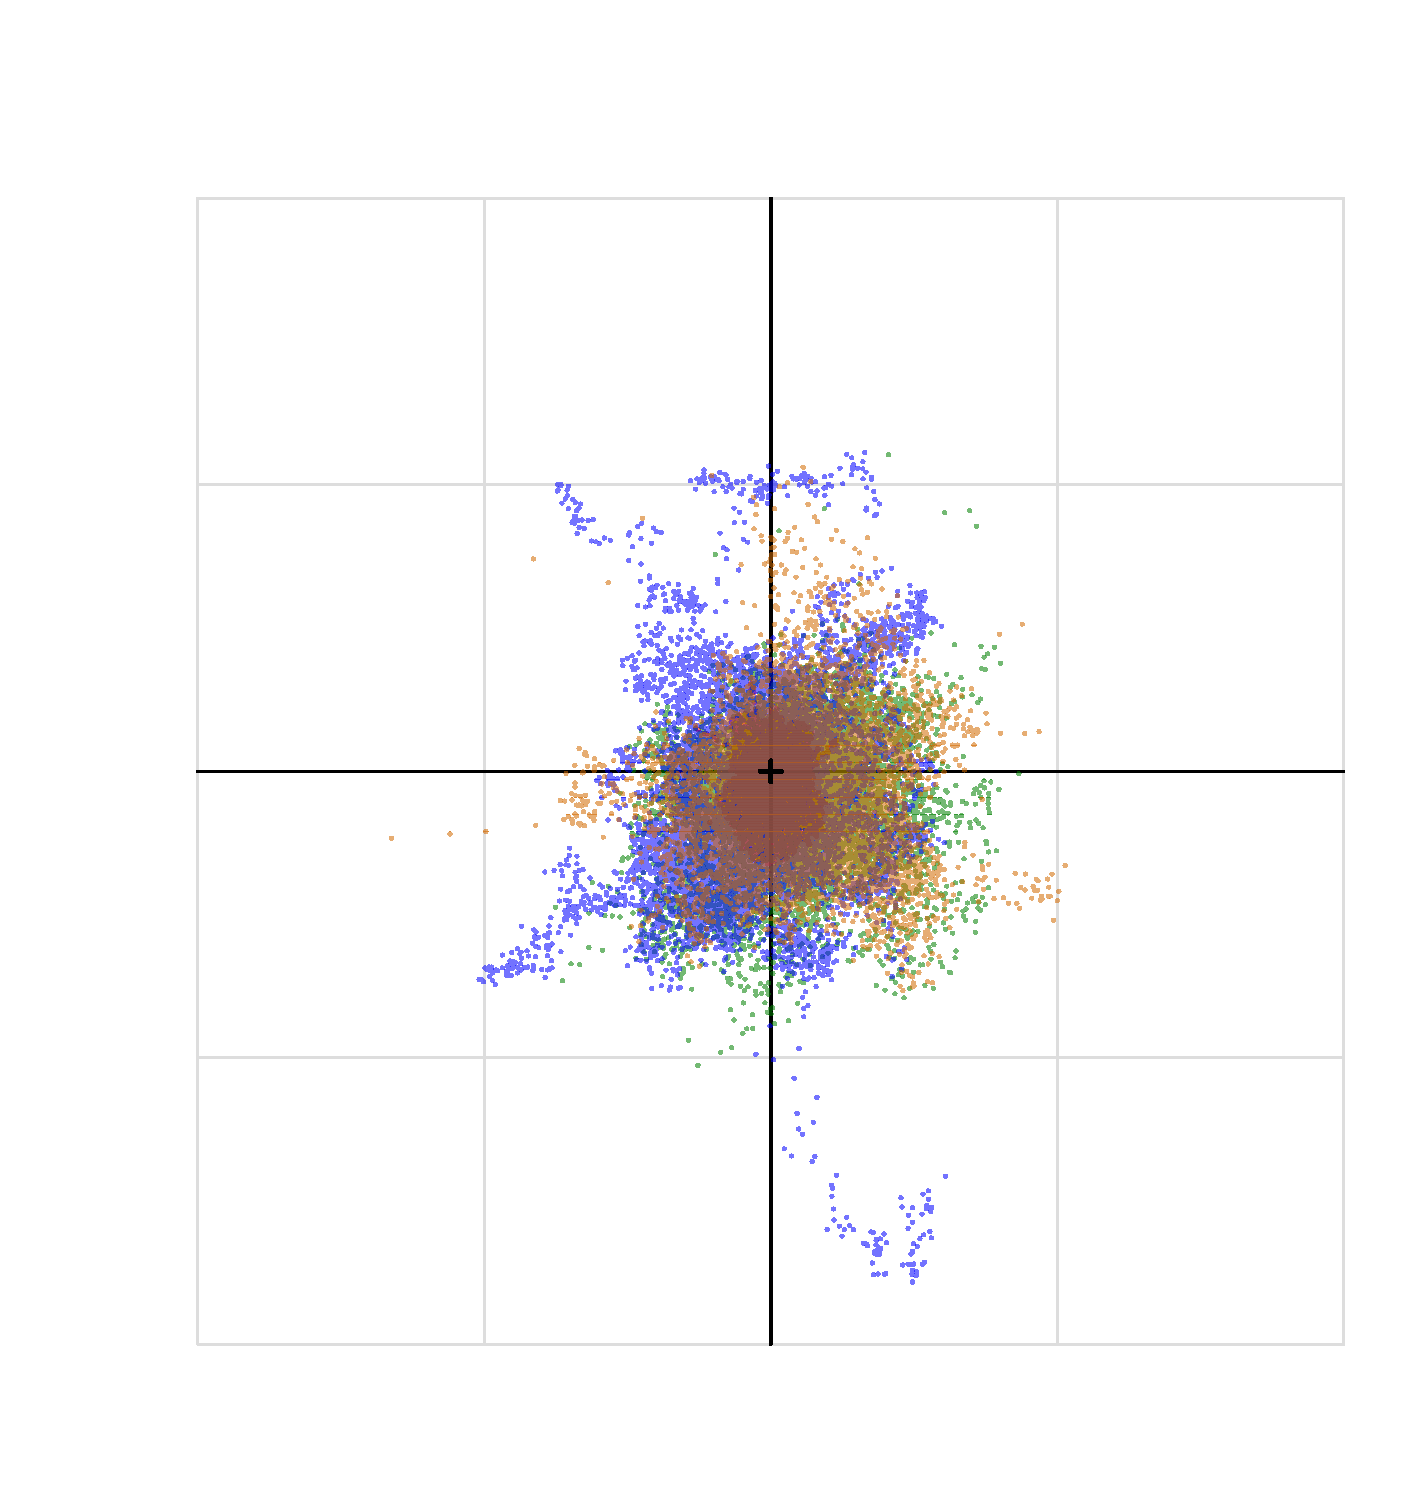
\includegraphics[width=680.0bp,height=715.0bp]{figures/horizontal_zh.pdf}}
\put(95.0,692.0){\makebox(0,0)[lb]{\color{black}\sffamily\fontsize{16}{16}\selectfont {\cjkfont 相}\allowbreak{}{\cjkfont 对}\allowbreak{}{\cjkfont 于}\allowbreak{}{\cjkfont 同}\allowbreak{}{\cjkfont 一}\allowbreak{}{\cjkfont 时}\allowbreak{}{\cjkfont 刻}\allowbreak{}{\cjkfont 理}\allowbreak{}{\cjkfont 论}\allowbreak{}{\cjkfont 圆}\allowbreak{}{\cjkfont 周}\allowbreak{}{\cjkfont 位}\allowbreak{}{\cjkfont 置}\allowbreak{}{\cjkfont 的}\allowbreak{}{\cjkfont 水}\allowbreak{}{\cjkfont 平}\allowbreak{}{\cjkfont 误}\allowbreak{}{\cjkfont 差}\allowbreak{}}}
\put(95.0,50.0){\makebox(0,0)[cb]{\color{black}\sffamily\fontsize{12}{12}\selectfont -0.1}}
\put(232.5,50.0){\makebox(0,0)[cb]{\color{black}\sffamily\fontsize{12}{12}\selectfont -0.05}}
\put(370.0,50.0){\makebox(0,0)[cb]{\color{black}\sffamily\fontsize{12}{12}\selectfont 0}}
\put(507.50000000000006,50.0){\makebox(0,0)[cb]{\color{black}\sffamily\fontsize{12}{12}\selectfont 0.05}}
\put(645.0,50.0){\makebox(0,0)[cb]{\color{black}\sffamily\fontsize{12}{12}\selectfont 0.1}}
\put(87.0,66.0){\makebox(0,0)[rb]{\color{black}\sffamily\fontsize{12}{12}\selectfont -0.1}}
\put(87.0,203.5){\makebox(0,0)[rb]{\color{black}\sffamily\fontsize{12}{12}\selectfont -0.05}}
\put(87.0,341.0){\makebox(0,0)[rb]{\color{black}\sffamily\fontsize{12}{12}\selectfont 0}}
\put(87.0,478.50000000000006){\makebox(0,0)[rb]{\color{black}\sffamily\fontsize{12}{12}\selectfont 0.05}}
\put(87.0,616.0){\makebox(0,0)[rb]{\color{black}\sffamily\fontsize{12}{12}\selectfont 0.1}}
\put(95.0,670.0){\makebox(0,0)[lb]{\color{red}\sffamily\fontsize{12}{12}\selectfont P23M\_0}}
\put(370.0,670.0){\makebox(0,0)[lb]{\color{green}\sffamily\fontsize{12}{12}\selectfont P23M\_1}}
\put(95.0,648.0){\makebox(0,0)[lb]{\color{blue}\sffamily\fontsize{12}{12}\selectfont UM980}}
\put(370.0,648.0){\makebox(0,0)[lb]{\color[HTML]{d26900}\sffamily\fontsize{12}{12}\selectfont LG290P}}
\put(378.0,353.0){\makebox(0,0)[lb]{\color{black}\sffamily\fontsize{12}{12}\selectfont {\cjkfont 理}\allowbreak{}{\cjkfont 论}\allowbreak{}{\cjkfont 值}\allowbreak{} (0,0)}}
\put(370.0,12.0){\makebox(0,0)[cb]{\color{black}\sffamily\fontsize{12}{12}\selectfont {\cjkfont 东}\allowbreak{}{\cjkfont 向}\allowbreak{}{\cjkfont 误}\allowbreak{}{\cjkfont 差}\allowbreak{} [m]}}
\put(19.0,345.0){\rotatebox{90}{\makebox(0,0)[b]{\color{black}\sffamily\fontsize{12}{12}\selectfont {\cjkfont 北}\allowbreak{}{\cjkfont 向}\allowbreak{}{\cjkfont 误}\allowbreak{}{\cjkfont 差}\allowbreak{} [m]}}}
\end{picture}}
\end{figure}
\begin{figure}[p]\centering
\resizebox{0.98\linewidth}{!}{%
\setlength{\unitlength}{1bp}\begin{picture}(680.0,715.0)
\put(0,0){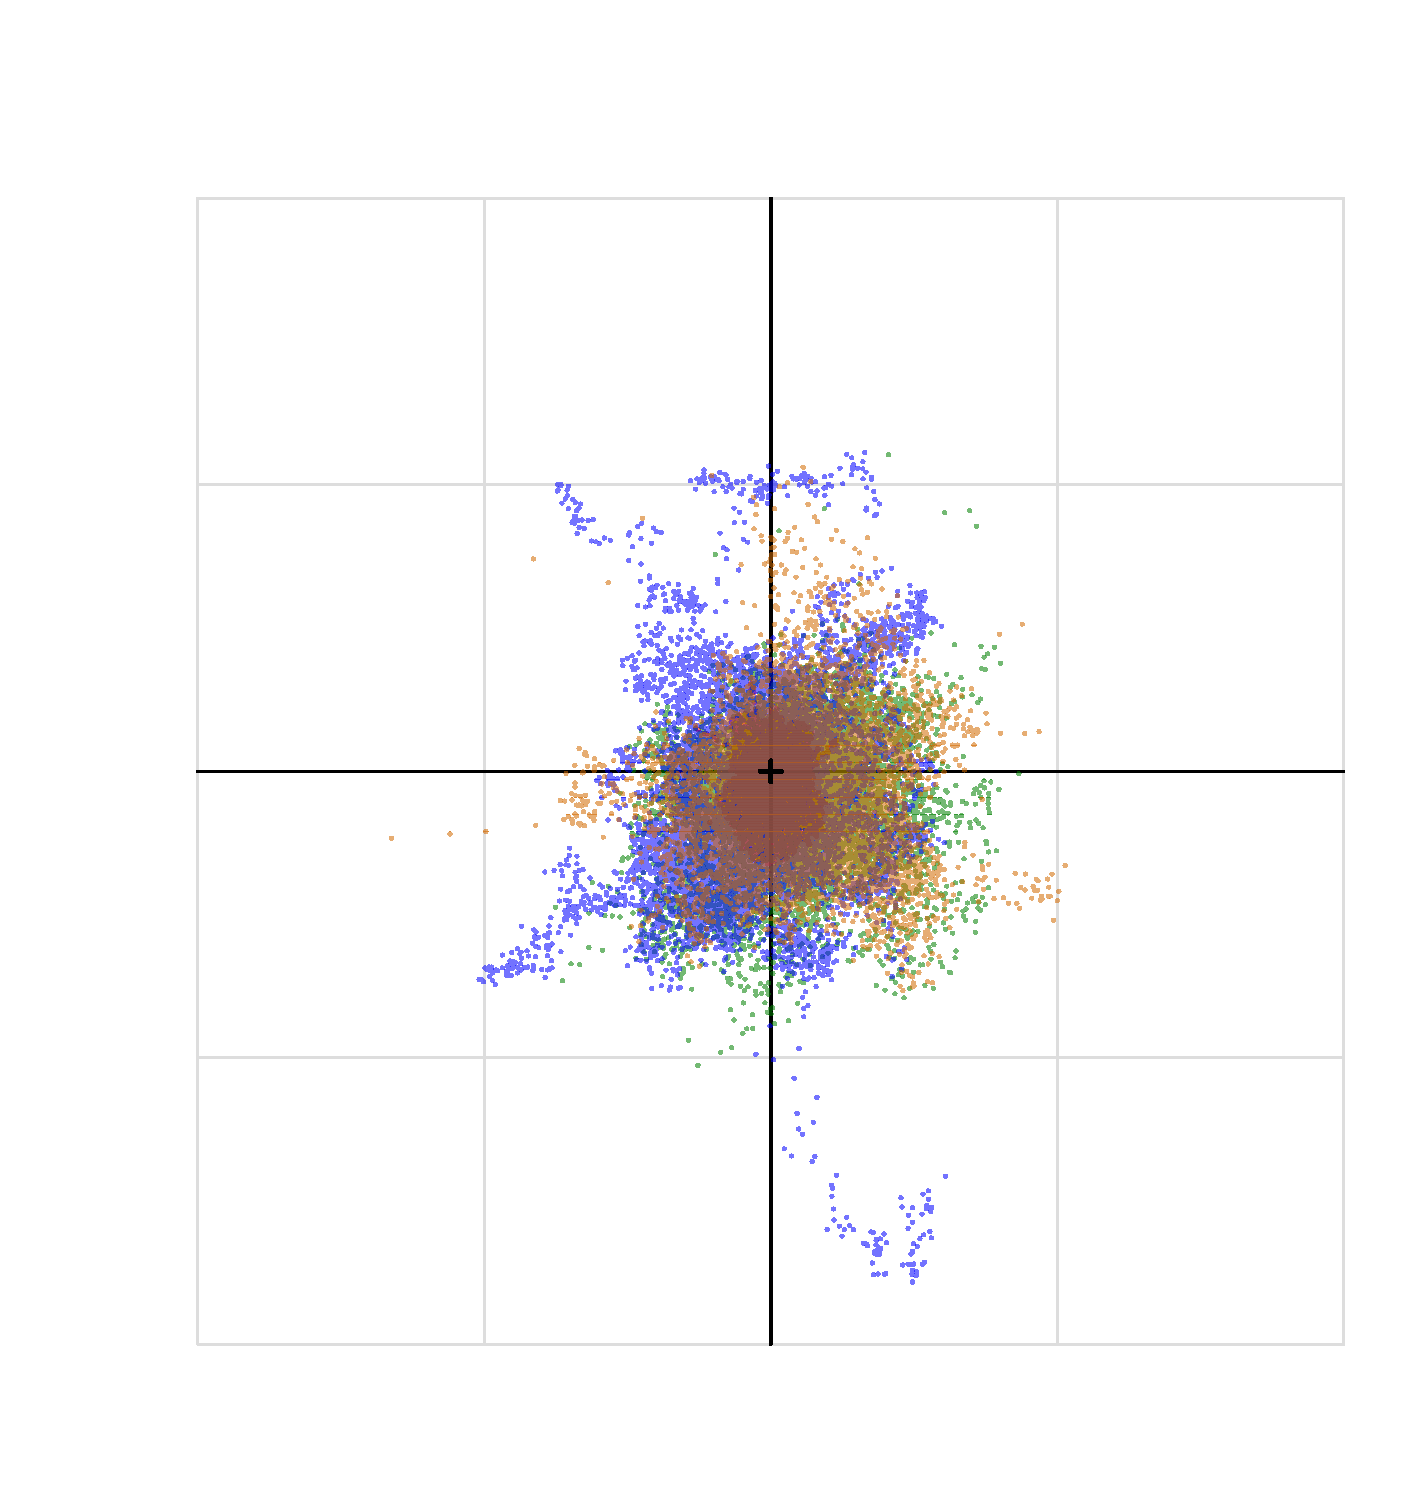
\includegraphics[width=680.0bp,height=715.0bp]{figures/horizontal_detail_zh.pdf}}
\put(95.0,692.0){\makebox(0,0)[lb]{\color{black}\sffamily\fontsize{16}{16}\selectfont {\cjkfont 局}\allowbreak{}{\cjkfont 部}\allowbreak{}{\cjkfont 视}\allowbreak{}{\cjkfont 图}\allowbreak{} ±0.10 m{\cjkfont （}\allowbreak{}{\cjkfont 不}\allowbreak{}{\cjkfont 显}\allowbreak{}{\cjkfont 示}\allowbreak{}{\cjkfont 范}\allowbreak{}{\cjkfont 围}\allowbreak{}{\cjkfont 外}\allowbreak{}{\cjkfont 的}\allowbreak{}{\cjkfont 误}\allowbreak{}{\cjkfont 差}\allowbreak{}{\cjkfont ）}\allowbreak{}}}
\put(95.0,50.0){\makebox(0,0)[cb]{\color{black}\sffamily\fontsize{12}{12}\selectfont -0.1}}
\put(232.5,50.0){\makebox(0,0)[cb]{\color{black}\sffamily\fontsize{12}{12}\selectfont -0.05}}
\put(370.0,50.0){\makebox(0,0)[cb]{\color{black}\sffamily\fontsize{12}{12}\selectfont 0}}
\put(507.50000000000006,50.0){\makebox(0,0)[cb]{\color{black}\sffamily\fontsize{12}{12}\selectfont 0.05}}
\put(645.0,50.0){\makebox(0,0)[cb]{\color{black}\sffamily\fontsize{12}{12}\selectfont 0.1}}
\put(87.0,66.0){\makebox(0,0)[rb]{\color{black}\sffamily\fontsize{12}{12}\selectfont -0.1}}
\put(87.0,203.5){\makebox(0,0)[rb]{\color{black}\sffamily\fontsize{12}{12}\selectfont -0.05}}
\put(87.0,341.0){\makebox(0,0)[rb]{\color{black}\sffamily\fontsize{12}{12}\selectfont 0}}
\put(87.0,478.50000000000006){\makebox(0,0)[rb]{\color{black}\sffamily\fontsize{12}{12}\selectfont 0.05}}
\put(87.0,616.0){\makebox(0,0)[rb]{\color{black}\sffamily\fontsize{12}{12}\selectfont 0.1}}
\put(95.0,670.0){\makebox(0,0)[lb]{\color{red}\sffamily\fontsize{12}{12}\selectfont P23M\_0}}
\put(370.0,670.0){\makebox(0,0)[lb]{\color{green}\sffamily\fontsize{12}{12}\selectfont P23M\_1}}
\put(95.0,648.0){\makebox(0,0)[lb]{\color{blue}\sffamily\fontsize{12}{12}\selectfont UM980}}
\put(370.0,648.0){\makebox(0,0)[lb]{\color[HTML]{d26900}\sffamily\fontsize{12}{12}\selectfont LG290P}}
\put(378.0,353.0){\makebox(0,0)[lb]{\color{black}\sffamily\fontsize{12}{12}\selectfont {\cjkfont 理}\allowbreak{}{\cjkfont 论}\allowbreak{}{\cjkfont 值}\allowbreak{} (0,0)}}
\put(370.0,12.0){\makebox(0,0)[cb]{\color{black}\sffamily\fontsize{12}{12}\selectfont {\cjkfont 东}\allowbreak{}{\cjkfont 向}\allowbreak{}{\cjkfont 误}\allowbreak{}{\cjkfont 差}\allowbreak{} [m]}}
\put(19.0,345.0){\rotatebox{90}{\makebox(0,0)[b]{\color{black}\sffamily\fontsize{12}{12}\selectfont {\cjkfont 北}\allowbreak{}{\cjkfont 向}\allowbreak{}{\cjkfont 误}\allowbreak{}{\cjkfont 差}\allowbreak{} [m]}}}
\end{picture}}
\end{figure}
\begin{figure}[p]\centering
\resizebox{0.98\linewidth}{!}{%
\setlength{\unitlength}{1bp}\begin{picture}(1000.0,430.0)
\put(0,0){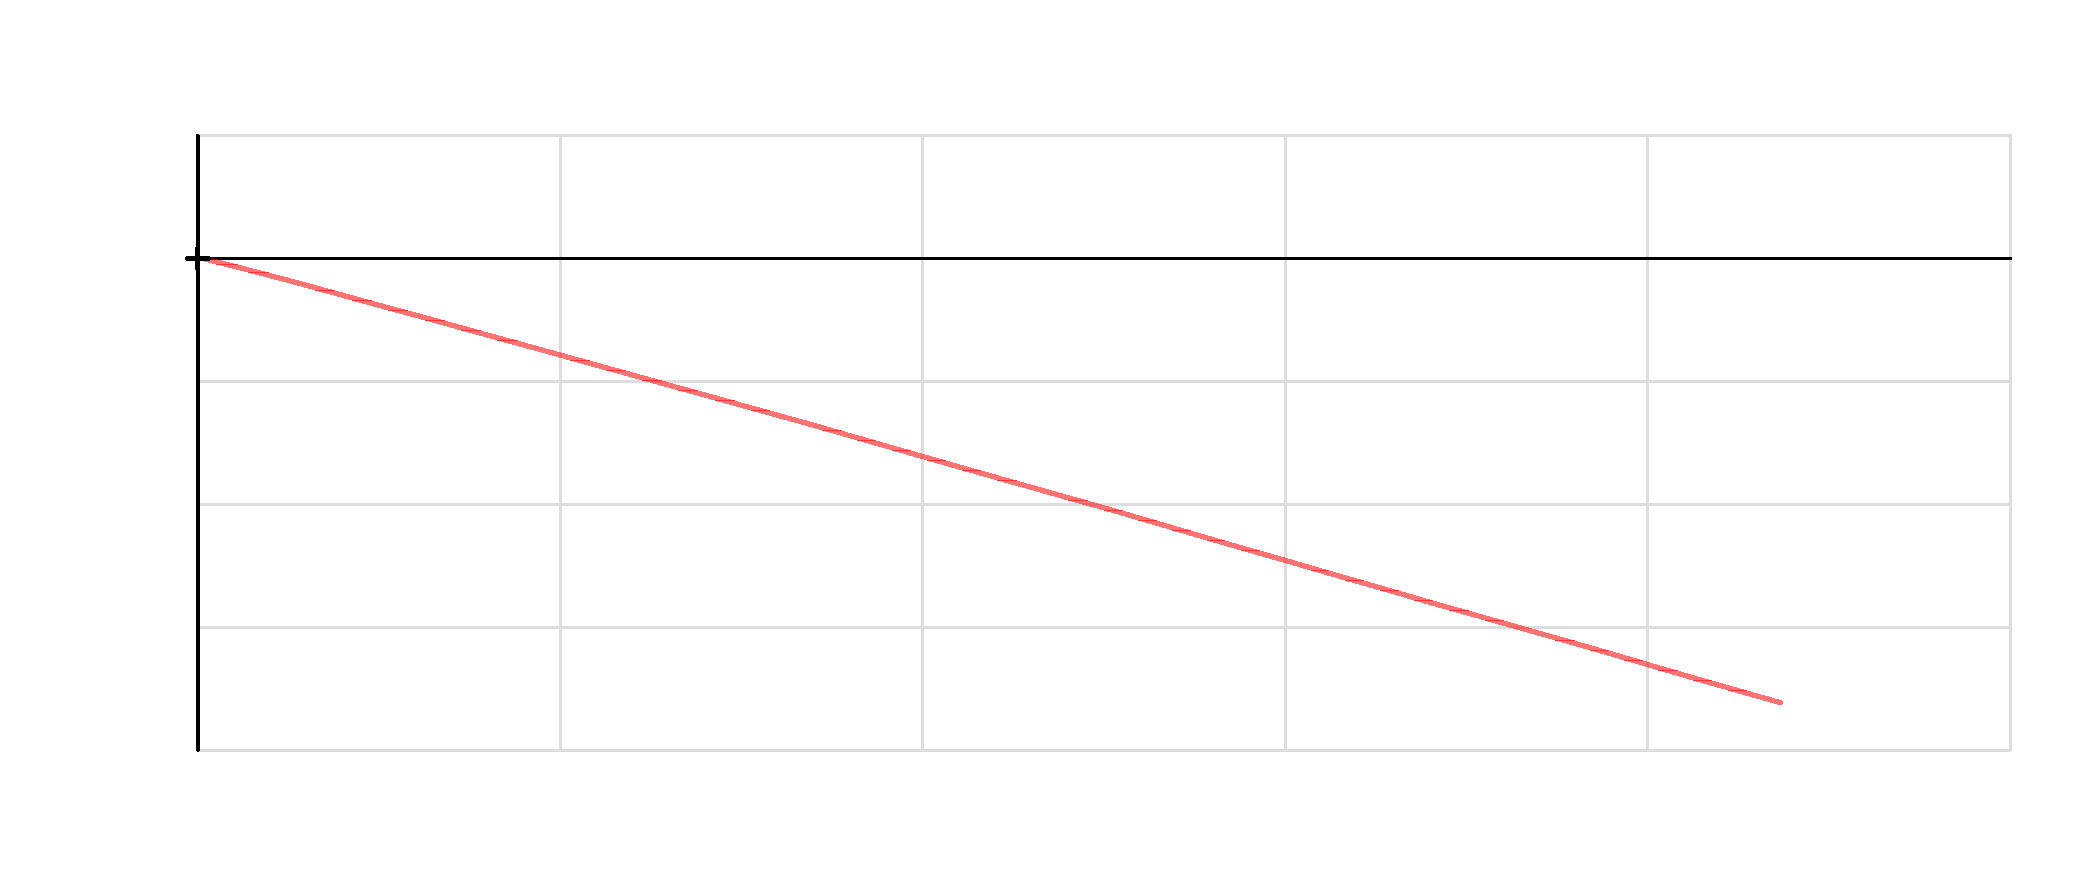
\includegraphics[width=1000.0bp,height=430.0bp]{figures/rotation_zh.pdf}}
\put(95.0,407.0){\makebox(0,0)[lb]{\color{black}\sffamily\fontsize{16}{16}\selectfont {\cjkfont 旋}\allowbreak{}{\cjkfont 转}\allowbreak{}{\cjkfont 圈}\allowbreak{}{\cjkfont 数}\allowbreak{}{\cjkfont ：}\allowbreak{}{\cjkfont 从}\allowbreak{}{\cjkfont 东}\allowbreak{}{\cjkfont 向}\allowbreak{}{\cjkfont 北}\allowbreak{}{\cjkfont 为}\allowbreak{}{\cjkfont 正}\allowbreak{}{\cjkfont 方}\allowbreak{}{\cjkfont 向}\allowbreak{}}}
\put(95.0,50.0){\makebox(0,0)[cb]{\color{black}\sffamily\fontsize{12}{12}\selectfont 0}}
\put(269.0,50.0){\makebox(0,0)[cb]{\color{black}\sffamily\fontsize{12}{12}\selectfont 50}}
\put(443.0,50.0){\makebox(0,0)[cb]{\color{black}\sffamily\fontsize{12}{12}\selectfont 100}}
\put(617.0,50.0){\makebox(0,0)[cb]{\color{black}\sffamily\fontsize{12}{12}\selectfont 150}}
\put(791.0,50.0){\makebox(0,0)[cb]{\color{black}\sffamily\fontsize{12}{12}\selectfont 200}}
\put(965.0,50.0){\makebox(0,0)[cb]{\color{black}\sffamily\fontsize{12}{12}\selectfont 250}}
\put(87.0,66.0){\makebox(0,0)[rb]{\color{black}\sffamily\fontsize{12}{12}\selectfont -80}}
\put(87.0,125.0){\makebox(0,0)[rb]{\color{black}\sffamily\fontsize{12}{12}\selectfont -60}}
\put(87.0,184.0){\makebox(0,0)[rb]{\color{black}\sffamily\fontsize{12}{12}\selectfont -40}}
\put(87.0,243.0){\makebox(0,0)[rb]{\color{black}\sffamily\fontsize{12}{12}\selectfont -20}}
\put(87.0,302.0){\makebox(0,0)[rb]{\color{black}\sffamily\fontsize{12}{12}\selectfont 0}}
\put(87.0,361.0){\makebox(0,0)[rb]{\color{black}\sffamily\fontsize{12}{12}\selectfont 20}}
\put(95.0,385.0){\makebox(0,0)[lb]{\color{red}\sffamily\fontsize{12}{12}\selectfont P23M\_0}}
\put(103.0,314.0){\makebox(0,0)[lb]{\color{black}\sffamily\fontsize{12}{12}\selectfont (0,0)}}
\put(530.0,12.0){\makebox(0,0)[cb]{\color{black}\sffamily\fontsize{12}{12}\selectfont {\cjkfont 自}\allowbreak{}{\cjkfont 共}\allowbreak{}{\cjkfont 同}\allowbreak{}{\cjkfont 起}\allowbreak{}{\cjkfont 始}\allowbreak{}{\cjkfont 时}\allowbreak{}{\cjkfont 刻}\allowbreak{}{\cjkfont 起}\allowbreak{}{\cjkfont 的}\allowbreak{}{\cjkfont 时}\allowbreak{}{\cjkfont 间}\allowbreak{} [min]}}
\put(19.0,217.5){\rotatebox{90}{\makebox(0,0)[b]{\color{black}\sffamily\fontsize{12}{12}\selectfont {\cjkfont 自}\allowbreak{}{\cjkfont 首}\allowbreak{}{\cjkfont 个}\allowbreak{}{\cjkfont 参}\allowbreak{}{\cjkfont 考}\allowbreak{}{\cjkfont 点}\allowbreak{}{\cjkfont 起}\allowbreak{}{\cjkfont 的}\allowbreak{}{\cjkfont 旋}\allowbreak{}{\cjkfont 转}\allowbreak{}{\cjkfont 圈}\allowbreak{}{\cjkfont 数}\allowbreak{}}}}
\end{picture}}
\end{figure}
\begin{figure}[p]\centering
\resizebox{0.98\linewidth}{!}{%
\setlength{\unitlength}{1bp}\begin{picture}(1000.0,435.0)
\put(0,0){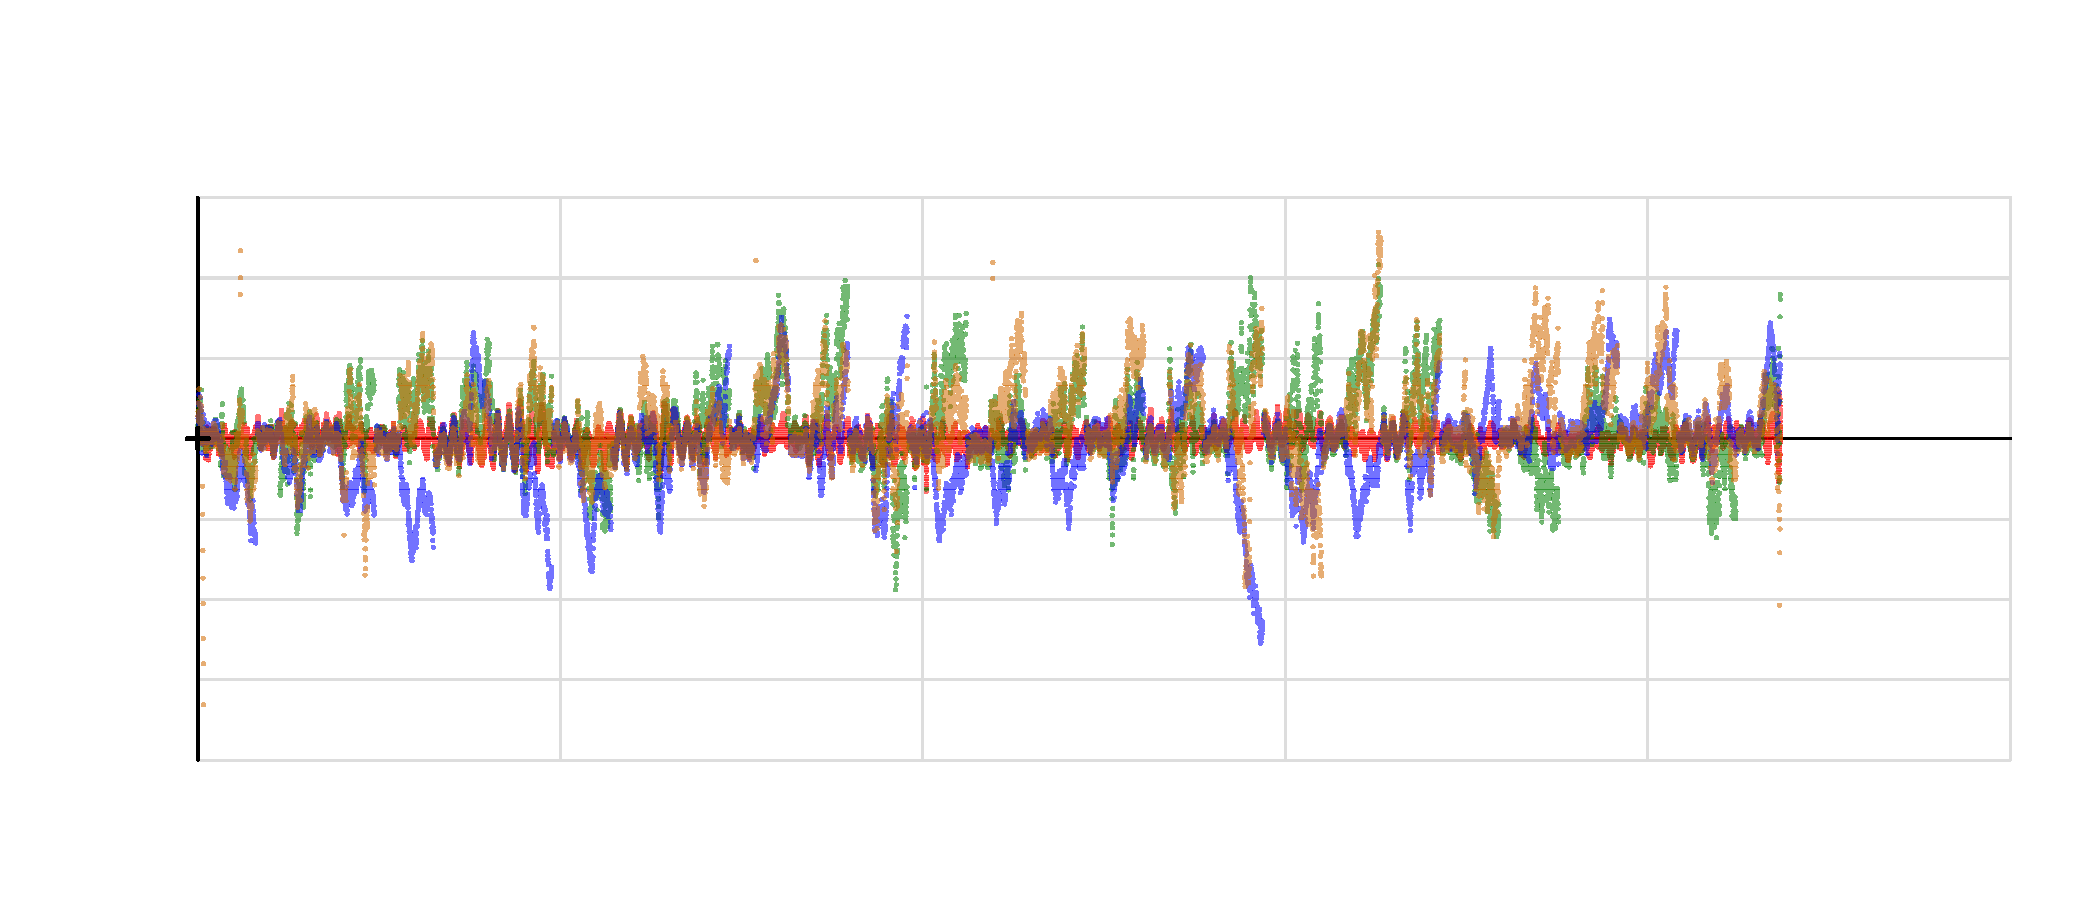
\includegraphics[width=1000.0bp,height=435.0bp]{figures/east_time_zh.pdf}}
\put(95.0,412.0){\makebox(0,0)[lb]{\color{black}\sffamily\fontsize{16}{16}\selectfont {\cjkfont 东}\allowbreak{}{\cjkfont 向}\allowbreak{}{\cjkfont 误}\allowbreak{}{\cjkfont 差}\allowbreak{}{\cjkfont 随}\allowbreak{}{\cjkfont 时}\allowbreak{}{\cjkfont 间}\allowbreak{}{\cjkfont 的}\allowbreak{}{\cjkfont 变}\allowbreak{}{\cjkfont 化}\allowbreak{}}}
\put(95.0,50.0){\makebox(0,0)[cb]{\color{black}\sffamily\fontsize{12}{12}\selectfont 0}}
\put(269.0,50.0){\makebox(0,0)[cb]{\color{black}\sffamily\fontsize{12}{12}\selectfont 50}}
\put(443.0,50.0){\makebox(0,0)[cb]{\color{black}\sffamily\fontsize{12}{12}\selectfont 100}}
\put(617.0,50.0){\makebox(0,0)[cb]{\color{black}\sffamily\fontsize{12}{12}\selectfont 150}}
\put(791.0,50.0){\makebox(0,0)[cb]{\color{black}\sffamily\fontsize{12}{12}\selectfont 200}}
\put(965.0,50.0){\makebox(0,0)[cb]{\color{black}\sffamily\fontsize{12}{12}\selectfont 250}}
\put(87.0,66.0){\makebox(0,0)[rb]{\color{black}\sffamily\fontsize{12}{12}\selectfont -0.08}}
\put(87.0,104.57142857142856){\makebox(0,0)[rb]{\color{black}\sffamily\fontsize{12}{12}\selectfont -0.06}}
\put(87.0,143.1428571428571){\makebox(0,0)[rb]{\color{black}\sffamily\fontsize{12}{12}\selectfont -0.04}}
\put(87.0,181.7142857142857){\makebox(0,0)[rb]{\color{black}\sffamily\fontsize{12}{12}\selectfont -0.02}}
\put(87.0,220.28571428571428){\makebox(0,0)[rb]{\color{black}\sffamily\fontsize{12}{12}\selectfont 0}}
\put(87.0,258.8571428571429){\makebox(0,0)[rb]{\color{black}\sffamily\fontsize{12}{12}\selectfont 0.02}}
\put(87.0,297.4285714285714){\makebox(0,0)[rb]{\color{black}\sffamily\fontsize{12}{12}\selectfont 0.04}}
\put(87.0,336.0){\makebox(0,0)[rb]{\color{black}\sffamily\fontsize{12}{12}\selectfont 0.06}}
\put(95.0,390.0){\makebox(0,0)[lb]{\color{red}\sffamily\fontsize{12}{12}\selectfont P23M\_0}}
\put(530.0,390.0){\makebox(0,0)[lb]{\color{green}\sffamily\fontsize{12}{12}\selectfont P23M\_1}}
\put(95.0,368.0){\makebox(0,0)[lb]{\color{blue}\sffamily\fontsize{12}{12}\selectfont UM980}}
\put(530.0,368.0){\makebox(0,0)[lb]{\color[HTML]{d26900}\sffamily\fontsize{12}{12}\selectfont LG290P}}
\put(103.0,232.28571428571428){\makebox(0,0)[lb]{\color{black}\sffamily\fontsize{12}{12}\selectfont (0,0)}}
\put(530.0,12.0){\makebox(0,0)[cb]{\color{black}\sffamily\fontsize{12}{12}\selectfont {\cjkfont 自}\allowbreak{}{\cjkfont 共}\allowbreak{}{\cjkfont 同}\allowbreak{}{\cjkfont 起}\allowbreak{}{\cjkfont 始}\allowbreak{}{\cjkfont 时}\allowbreak{}{\cjkfont 刻}\allowbreak{}{\cjkfont 起}\allowbreak{}{\cjkfont 的}\allowbreak{}{\cjkfont 时}\allowbreak{}{\cjkfont 间}\allowbreak{} [min]}}
\put(19.0,205.0){\rotatebox{90}{\makebox(0,0)[b]{\color{black}\sffamily\fontsize{12}{12}\selectfont {\cjkfont 东}\allowbreak{}{\cjkfont 向}\allowbreak{}{\cjkfont 误}\allowbreak{}{\cjkfont 差}\allowbreak{} [m]}}}
\end{picture}}
\end{figure}
\begin{figure}[p]\centering
\resizebox{0.98\linewidth}{!}{%
\setlength{\unitlength}{1bp}\begin{picture}(1000.0,435.0)
\put(0,0){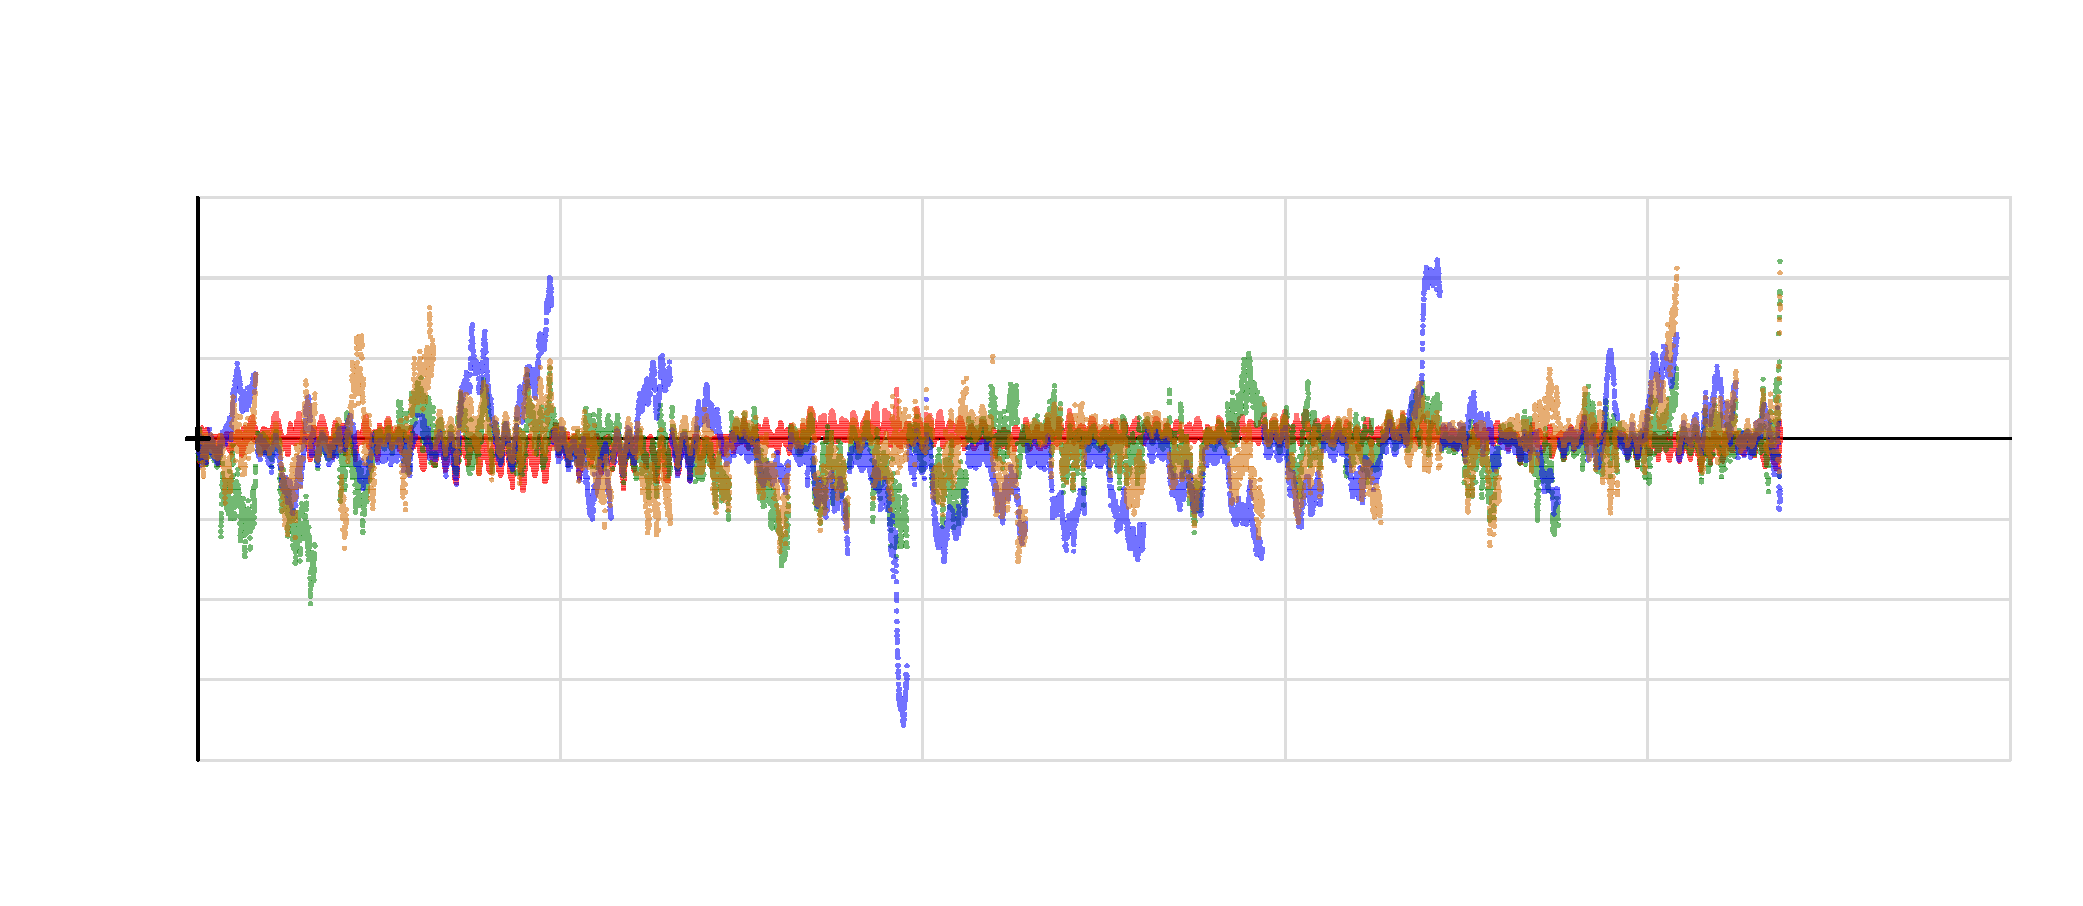
\includegraphics[width=1000.0bp,height=435.0bp]{figures/north_time_zh.pdf}}
\put(95.0,412.0){\makebox(0,0)[lb]{\color{black}\sffamily\fontsize{16}{16}\selectfont {\cjkfont 北}\allowbreak{}{\cjkfont 向}\allowbreak{}{\cjkfont 误}\allowbreak{}{\cjkfont 差}\allowbreak{}{\cjkfont 随}\allowbreak{}{\cjkfont 时}\allowbreak{}{\cjkfont 间}\allowbreak{}{\cjkfont 的}\allowbreak{}{\cjkfont 变}\allowbreak{}{\cjkfont 化}\allowbreak{}}}
\put(95.0,50.0){\makebox(0,0)[cb]{\color{black}\sffamily\fontsize{12}{12}\selectfont 0}}
\put(269.0,50.0){\makebox(0,0)[cb]{\color{black}\sffamily\fontsize{12}{12}\selectfont 50}}
\put(443.0,50.0){\makebox(0,0)[cb]{\color{black}\sffamily\fontsize{12}{12}\selectfont 100}}
\put(617.0,50.0){\makebox(0,0)[cb]{\color{black}\sffamily\fontsize{12}{12}\selectfont 150}}
\put(791.0,50.0){\makebox(0,0)[cb]{\color{black}\sffamily\fontsize{12}{12}\selectfont 200}}
\put(965.0,50.0){\makebox(0,0)[cb]{\color{black}\sffamily\fontsize{12}{12}\selectfont 250}}
\put(87.0,66.0){\makebox(0,0)[rb]{\color{black}\sffamily\fontsize{12}{12}\selectfont -0.1}}
\put(87.0,104.57142857142856){\makebox(0,0)[rb]{\color{black}\sffamily\fontsize{12}{12}\selectfont -0.075}}
\put(87.0,143.1428571428571){\makebox(0,0)[rb]{\color{black}\sffamily\fontsize{12}{12}\selectfont -0.05}}
\put(87.0,181.71428571428572){\makebox(0,0)[rb]{\color{black}\sffamily\fontsize{12}{12}\selectfont -0.025}}
\put(87.0,220.28571428571428){\makebox(0,0)[rb]{\color{black}\sffamily\fontsize{12}{12}\selectfont 0}}
\put(87.0,258.85714285714283){\makebox(0,0)[rb]{\color{black}\sffamily\fontsize{12}{12}\selectfont 0.025}}
\put(87.0,297.42857142857144){\makebox(0,0)[rb]{\color{black}\sffamily\fontsize{12}{12}\selectfont 0.05}}
\put(87.0,336.0){\makebox(0,0)[rb]{\color{black}\sffamily\fontsize{12}{12}\selectfont 0.075}}
\put(95.0,390.0){\makebox(0,0)[lb]{\color{red}\sffamily\fontsize{12}{12}\selectfont P23M\_0}}
\put(530.0,390.0){\makebox(0,0)[lb]{\color{green}\sffamily\fontsize{12}{12}\selectfont P23M\_1}}
\put(95.0,368.0){\makebox(0,0)[lb]{\color{blue}\sffamily\fontsize{12}{12}\selectfont UM980}}
\put(530.0,368.0){\makebox(0,0)[lb]{\color[HTML]{d26900}\sffamily\fontsize{12}{12}\selectfont LG290P}}
\put(103.0,232.28571428571428){\makebox(0,0)[lb]{\color{black}\sffamily\fontsize{12}{12}\selectfont (0,0)}}
\put(530.0,12.0){\makebox(0,0)[cb]{\color{black}\sffamily\fontsize{12}{12}\selectfont {\cjkfont 自}\allowbreak{}{\cjkfont 共}\allowbreak{}{\cjkfont 同}\allowbreak{}{\cjkfont 起}\allowbreak{}{\cjkfont 始}\allowbreak{}{\cjkfont 时}\allowbreak{}{\cjkfont 刻}\allowbreak{}{\cjkfont 起}\allowbreak{}{\cjkfont 的}\allowbreak{}{\cjkfont 时}\allowbreak{}{\cjkfont 间}\allowbreak{} [min]}}
\put(19.0,205.0){\rotatebox{90}{\makebox(0,0)[b]{\color{black}\sffamily\fontsize{12}{12}\selectfont {\cjkfont 北}\allowbreak{}{\cjkfont 向}\allowbreak{}{\cjkfont 误}\allowbreak{}{\cjkfont 差}\allowbreak{} [m]}}}
\end{picture}}
\end{figure}
\begin{figure}[p]\centering
\resizebox{0.98\linewidth}{!}{%
\setlength{\unitlength}{1bp}\begin{picture}(1000.0,435.0)
\put(0,0){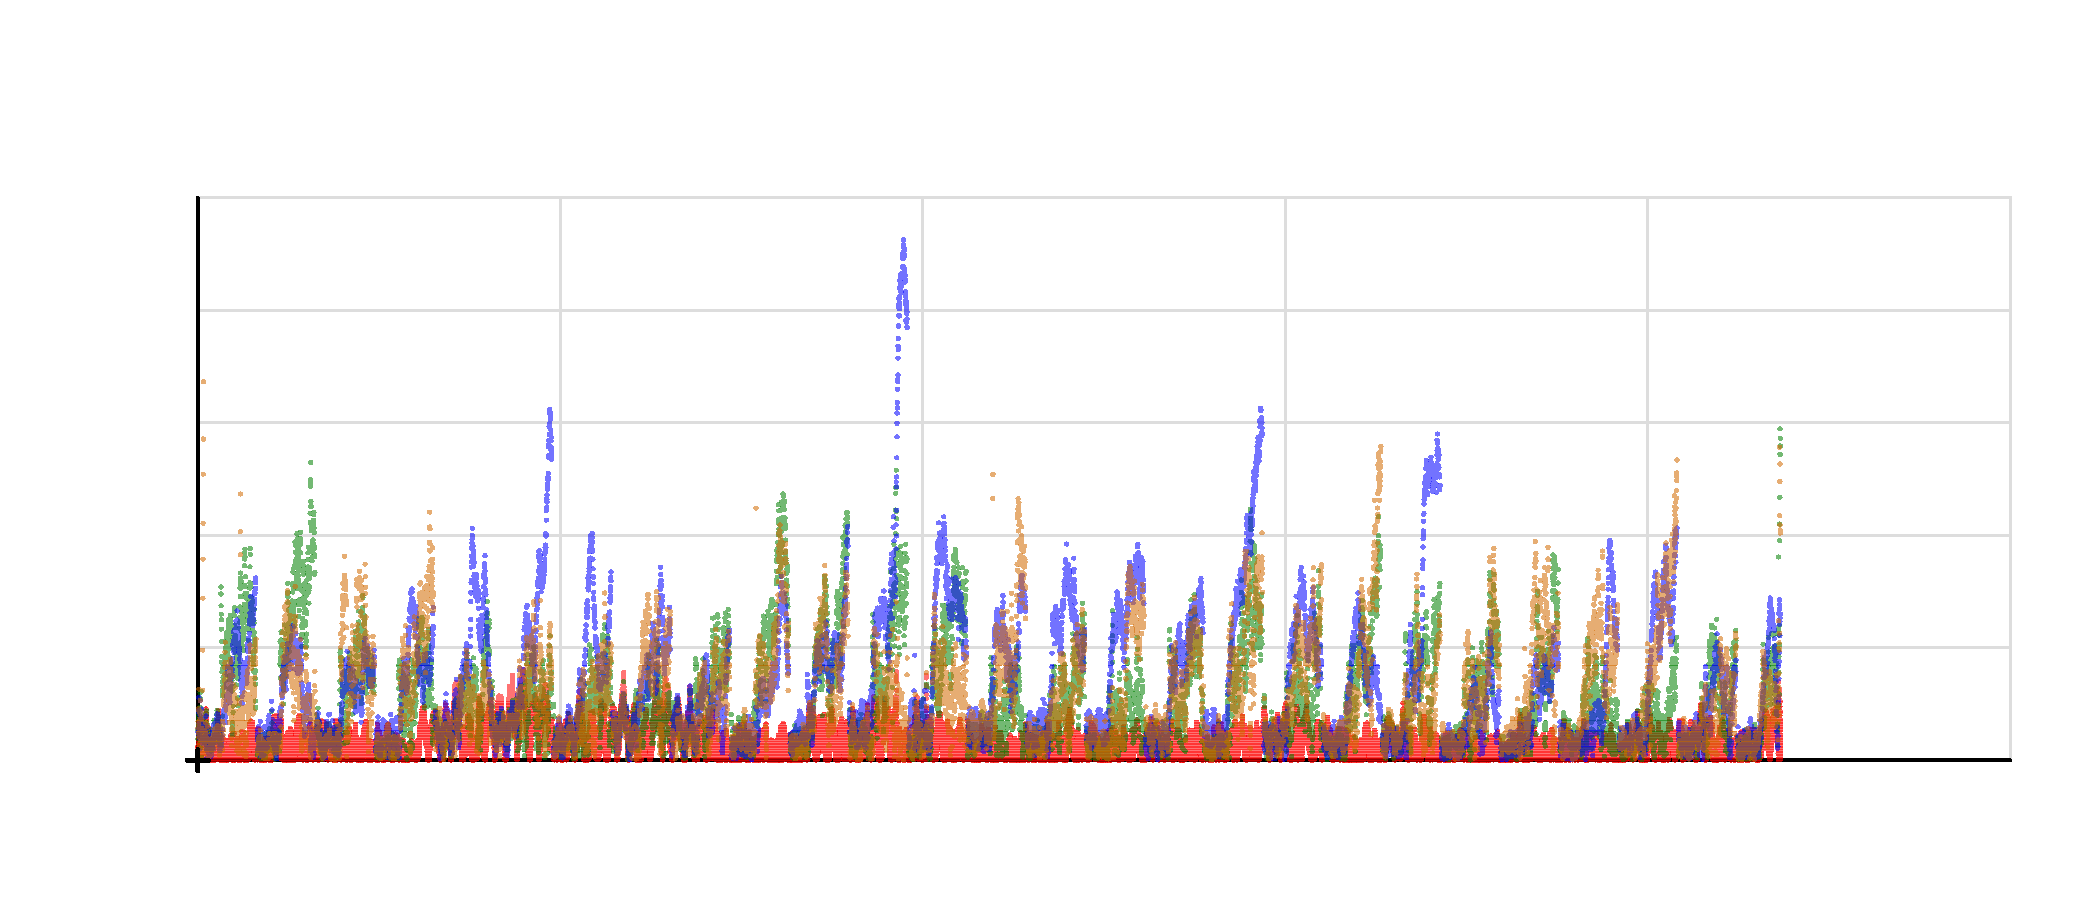
\includegraphics[width=1000.0bp,height=435.0bp]{figures/horizontal_time_zh.pdf}}
\put(95.0,412.0){\makebox(0,0)[lb]{\color{black}\sffamily\fontsize{16}{16}\selectfont {\cjkfont 水}\allowbreak{}{\cjkfont 平}\allowbreak{}{\cjkfont 误}\allowbreak{}{\cjkfont 差}\allowbreak{}{\cjkfont 随}\allowbreak{}{\cjkfont 时}\allowbreak{}{\cjkfont 间}\allowbreak{}{\cjkfont 的}\allowbreak{}{\cjkfont 变}\allowbreak{}{\cjkfont 化}\allowbreak{}}}
\put(95.0,50.0){\makebox(0,0)[cb]{\color{black}\sffamily\fontsize{12}{12}\selectfont 0}}
\put(269.0,50.0){\makebox(0,0)[cb]{\color{black}\sffamily\fontsize{12}{12}\selectfont 50}}
\put(443.0,50.0){\makebox(0,0)[cb]{\color{black}\sffamily\fontsize{12}{12}\selectfont 100}}
\put(617.0,50.0){\makebox(0,0)[cb]{\color{black}\sffamily\fontsize{12}{12}\selectfont 150}}
\put(791.0,50.0){\makebox(0,0)[cb]{\color{black}\sffamily\fontsize{12}{12}\selectfont 200}}
\put(965.0,50.0){\makebox(0,0)[cb]{\color{black}\sffamily\fontsize{12}{12}\selectfont 250}}
\put(87.0,66.0){\makebox(0,0)[rb]{\color{black}\sffamily\fontsize{12}{12}\selectfont 0}}
\put(87.0,120.0){\makebox(0,0)[rb]{\color{black}\sffamily\fontsize{12}{12}\selectfont 0.02}}
\put(87.0,174.0){\makebox(0,0)[rb]{\color{black}\sffamily\fontsize{12}{12}\selectfont 0.04}}
\put(87.0,228.0){\makebox(0,0)[rb]{\color{black}\sffamily\fontsize{12}{12}\selectfont 0.06}}
\put(87.0,282.0){\makebox(0,0)[rb]{\color{black}\sffamily\fontsize{12}{12}\selectfont 0.08}}
\put(87.0,336.0){\makebox(0,0)[rb]{\color{black}\sffamily\fontsize{12}{12}\selectfont 0.1}}
\put(95.0,390.0){\makebox(0,0)[lb]{\color{red}\sffamily\fontsize{12}{12}\selectfont P23M\_0}}
\put(530.0,390.0){\makebox(0,0)[lb]{\color{green}\sffamily\fontsize{12}{12}\selectfont P23M\_1}}
\put(95.0,368.0){\makebox(0,0)[lb]{\color{blue}\sffamily\fontsize{12}{12}\selectfont UM980}}
\put(530.0,368.0){\makebox(0,0)[lb]{\color[HTML]{d26900}\sffamily\fontsize{12}{12}\selectfont LG290P}}
\put(103.0,78.0){\makebox(0,0)[lb]{\color{black}\sffamily\fontsize{12}{12}\selectfont (0,0)}}
\put(530.0,12.0){\makebox(0,0)[cb]{\color{black}\sffamily\fontsize{12}{12}\selectfont {\cjkfont 自}\allowbreak{}{\cjkfont 共}\allowbreak{}{\cjkfont 同}\allowbreak{}{\cjkfont 起}\allowbreak{}{\cjkfont 始}\allowbreak{}{\cjkfont 时}\allowbreak{}{\cjkfont 刻}\allowbreak{}{\cjkfont 起}\allowbreak{}{\cjkfont 的}\allowbreak{}{\cjkfont 时}\allowbreak{}{\cjkfont 间}\allowbreak{} [min]}}
\put(19.0,205.0){\rotatebox{90}{\makebox(0,0)[b]{\color{black}\sffamily\fontsize{12}{12}\selectfont {\cjkfont 水}\allowbreak{}{\cjkfont 平}\allowbreak{}{\cjkfont 误}\allowbreak{}{\cjkfont 差}\allowbreak{} [m]}}}
\end{picture}}
\end{figure}
\begin{figure}[p]\centering
\resizebox{0.98\linewidth}{!}{%
\setlength{\unitlength}{1bp}\begin{picture}(1000.0,435.0)
\put(0,0){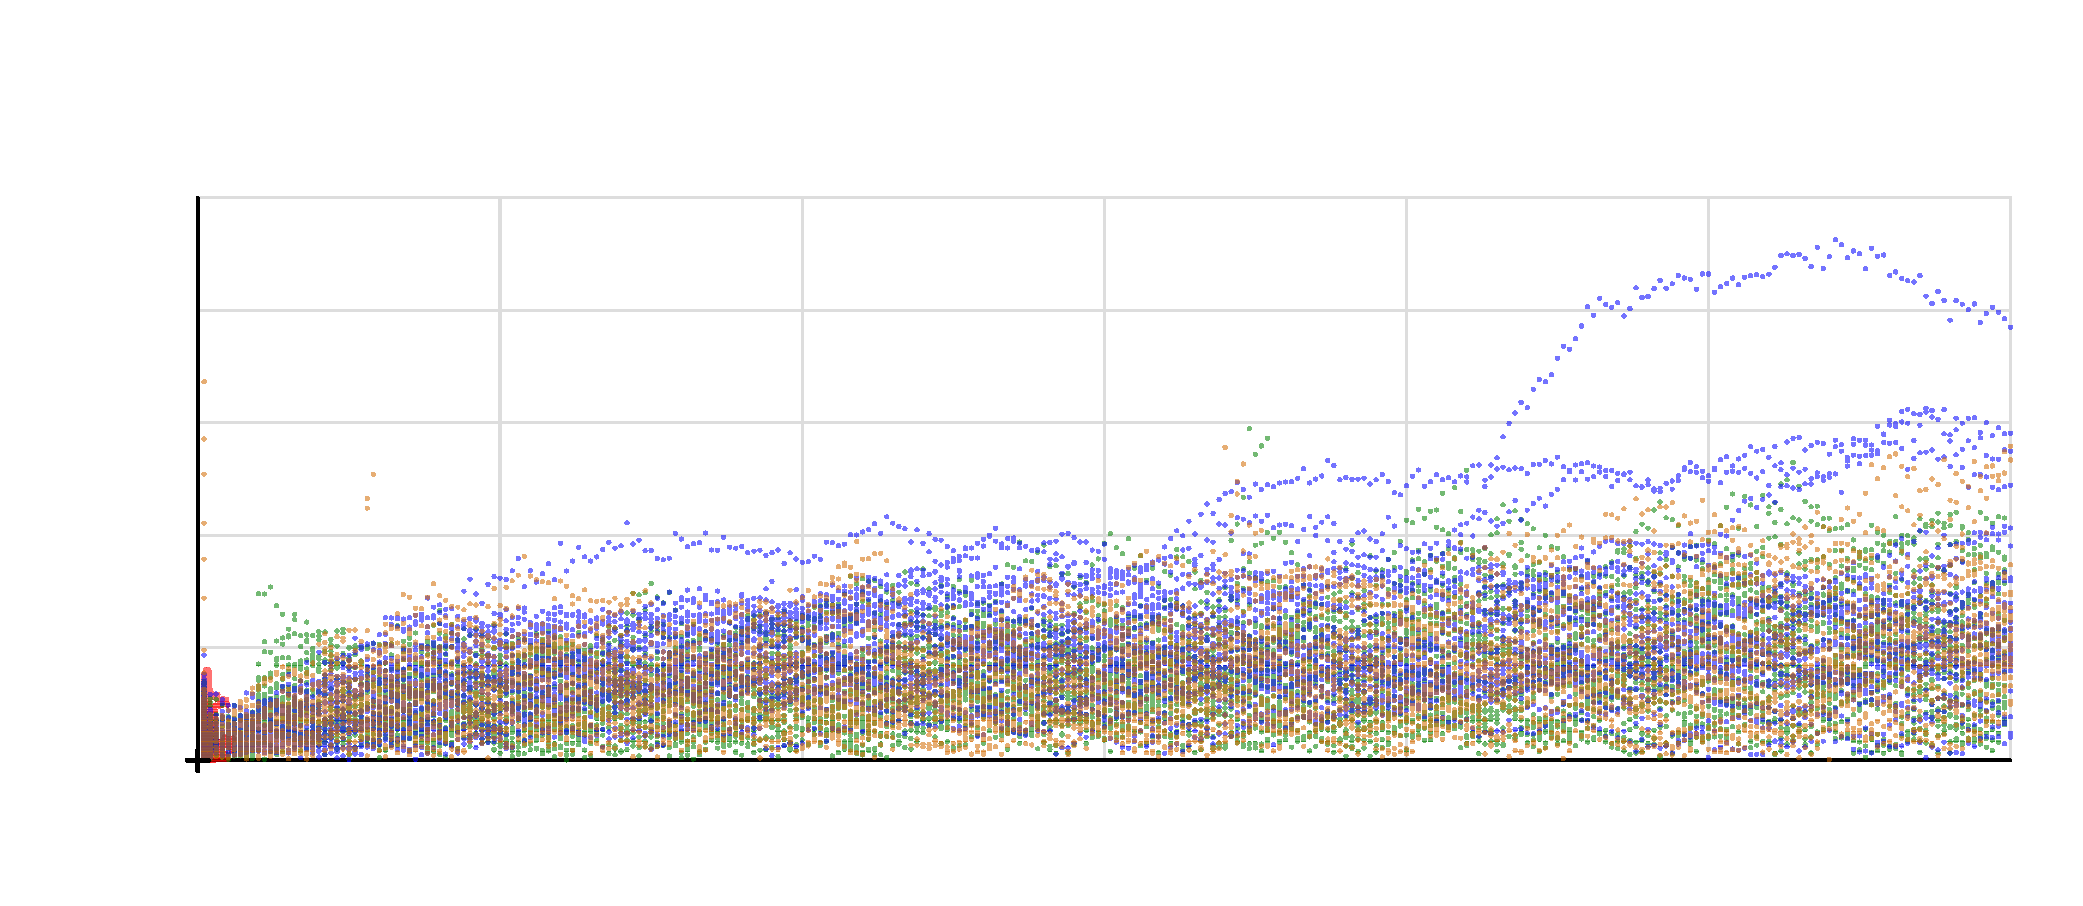
\includegraphics[width=1000.0bp,height=435.0bp]{figures/horizontal_dage_scatter_zh.pdf}}
\put(95.0,412.0){\makebox(0,0)[lb]{\color{black}\sffamily\fontsize{16}{16}\selectfont {\cjkfont 水}\allowbreak{}{\cjkfont 平}\allowbreak{}{\cjkfont 误}\allowbreak{}{\cjkfont 差}\allowbreak{}{\cjkfont 随}\allowbreak{} dAge {\cjkfont 的}\allowbreak{}{\cjkfont 变}\allowbreak{}{\cjkfont 化}\allowbreak{}{\cjkfont ：}\allowbreak{}{\cjkfont 全}\allowbreak{}{\cjkfont 部}\allowbreak{} RTK {\cjkfont 固}\allowbreak{}{\cjkfont 定}\allowbreak{}{\cjkfont 解}\allowbreak{}{\cjkfont 单}\allowbreak{}{\cjkfont 点}\allowbreak{}{\cjkfont 值}\allowbreak{}}}
\put(95.0,50.0){\makebox(0,0)[cb]{\color{black}\sffamily\fontsize{12}{12}\selectfont 0}}
\put(240.0,50.0){\makebox(0,0)[cb]{\color{black}\sffamily\fontsize{12}{12}\selectfont 50}}
\put(385.0,50.0){\makebox(0,0)[cb]{\color{black}\sffamily\fontsize{12}{12}\selectfont 100}}
\put(530.0,50.0){\makebox(0,0)[cb]{\color{black}\sffamily\fontsize{12}{12}\selectfont 150}}
\put(675.0,50.0){\makebox(0,0)[cb]{\color{black}\sffamily\fontsize{12}{12}\selectfont 200}}
\put(820.0,50.0){\makebox(0,0)[cb]{\color{black}\sffamily\fontsize{12}{12}\selectfont 250}}
\put(965.0,50.0){\makebox(0,0)[cb]{\color{black}\sffamily\fontsize{12}{12}\selectfont 300}}
\put(87.0,66.0){\makebox(0,0)[rb]{\color{black}\sffamily\fontsize{12}{12}\selectfont 0}}
\put(87.0,120.0){\makebox(0,0)[rb]{\color{black}\sffamily\fontsize{12}{12}\selectfont 20}}
\put(87.0,174.0){\makebox(0,0)[rb]{\color{black}\sffamily\fontsize{12}{12}\selectfont 40}}
\put(87.0,228.0){\makebox(0,0)[rb]{\color{black}\sffamily\fontsize{12}{12}\selectfont 60}}
\put(87.0,282.0){\makebox(0,0)[rb]{\color{black}\sffamily\fontsize{12}{12}\selectfont 80}}
\put(87.0,336.0){\makebox(0,0)[rb]{\color{black}\sffamily\fontsize{12}{12}\selectfont 100}}
\put(95.0,390.0){\makebox(0,0)[lb]{\color{red}\sffamily\fontsize{12}{12}\selectfont P23M\_0}}
\put(530.0,390.0){\makebox(0,0)[lb]{\color{green}\sffamily\fontsize{12}{12}\selectfont P23M\_1}}
\put(95.0,368.0){\makebox(0,0)[lb]{\color{blue}\sffamily\fontsize{12}{12}\selectfont UM980}}
\put(530.0,368.0){\makebox(0,0)[lb]{\color[HTML]{d26900}\sffamily\fontsize{12}{12}\selectfont LG290P}}
\put(103.0,78.0){\makebox(0,0)[lb]{\color{black}\sffamily\fontsize{12}{12}\selectfont (0,0)}}
\put(530.0,12.0){\makebox(0,0)[cb]{\color{black}\sffamily\fontsize{12}{12}\selectfont {\cjkfont 改}\allowbreak{}{\cjkfont 正}\allowbreak{}{\cjkfont 数}\allowbreak{}{\cjkfont 据}\allowbreak{}{\cjkfont 龄}\allowbreak{}{\cjkfont 期}\allowbreak{} dAge [s]}}
\put(19.0,205.0){\rotatebox{90}{\makebox(0,0)[b]{\color{black}\sffamily\fontsize{12}{12}\selectfont {\cjkfont 水}\allowbreak{}{\cjkfont 平}\allowbreak{}{\cjkfont 误}\allowbreak{}{\cjkfont 差}\allowbreak{} [mm]}}}
\end{picture}}
\end{figure}
\begin{figure}[p]\centering
\resizebox{0.98\linewidth}{!}{%
\setlength{\unitlength}{1bp}\begin{picture}(1000.0,479.0)
\put(0,0){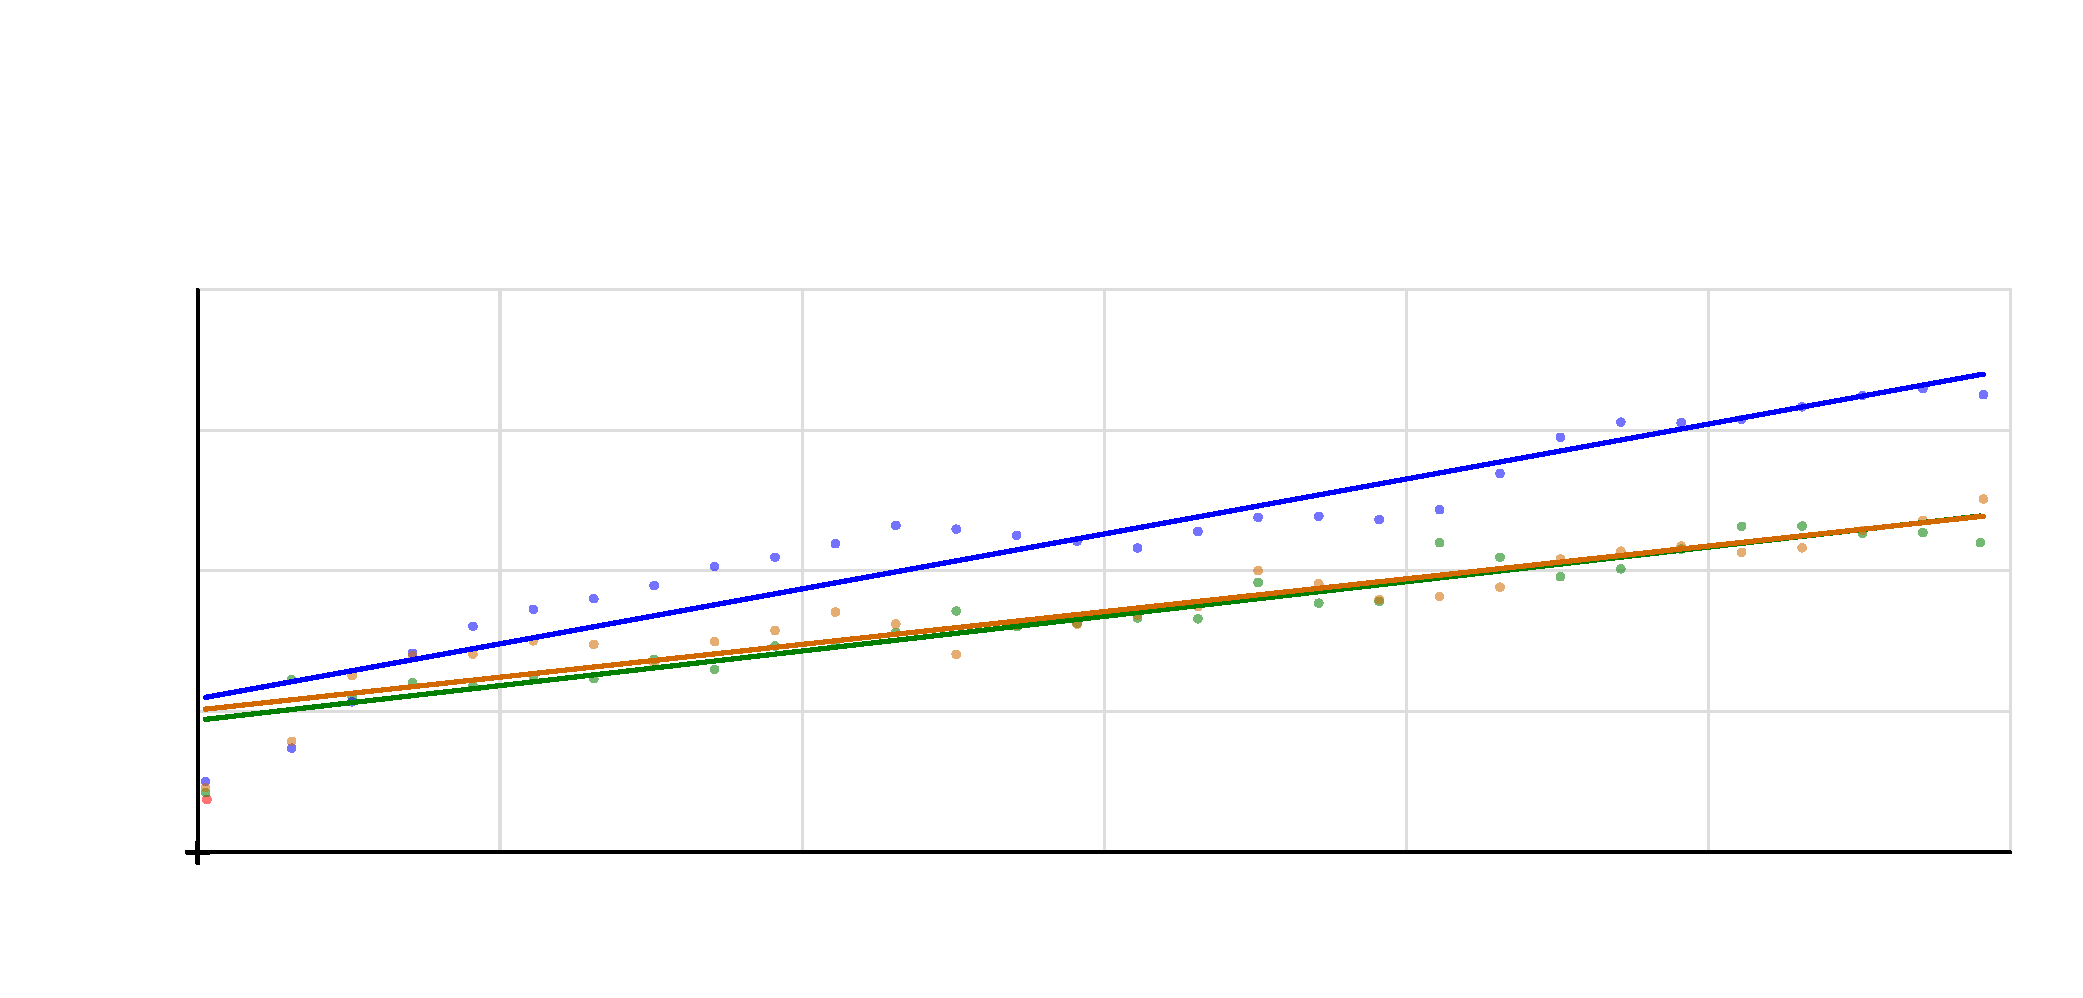
\includegraphics[width=1000.0bp,height=479.0bp]{figures/horizontal_dage_zh.pdf}}
\put(95.0,456.0){\makebox(0,0)[lb]{\color{black}\sffamily\fontsize{16}{16}\selectfont HRMS {\cjkfont 随}\allowbreak{} dAge {\cjkfont 的}\allowbreak{}{\cjkfont 变}\allowbreak{}{\cjkfont 化}\allowbreak{}{\cjkfont ：}\allowbreak{}10 {\cjkfont 秒}\allowbreak{}{\cjkfont 区}\allowbreak{}{\cjkfont 间}\allowbreak{}{\cjkfont 及}\allowbreak{}{\cjkfont 线}\allowbreak{}{\cjkfont 性}\allowbreak{}{\cjkfont 拟}\allowbreak{}{\cjkfont 合}\allowbreak{}}}
\put(95.0,50.0){\makebox(0,0)[cb]{\color{black}\sffamily\fontsize{12}{12}\selectfont 0}}
\put(240.0,50.0){\makebox(0,0)[cb]{\color{black}\sffamily\fontsize{12}{12}\selectfont 50}}
\put(385.0,50.0){\makebox(0,0)[cb]{\color{black}\sffamily\fontsize{12}{12}\selectfont 100}}
\put(530.0,50.0){\makebox(0,0)[cb]{\color{black}\sffamily\fontsize{12}{12}\selectfont 150}}
\put(675.0,50.0){\makebox(0,0)[cb]{\color{black}\sffamily\fontsize{12}{12}\selectfont 200}}
\put(820.0,50.0){\makebox(0,0)[cb]{\color{black}\sffamily\fontsize{12}{12}\selectfont 250}}
\put(965.0,50.0){\makebox(0,0)[cb]{\color{black}\sffamily\fontsize{12}{12}\selectfont 300}}
\put(87.0,66.0){\makebox(0,0)[rb]{\color{black}\sffamily\fontsize{12}{12}\selectfont 0}}
\put(87.0,133.5){\makebox(0,0)[rb]{\color{black}\sffamily\fontsize{12}{12}\selectfont 10}}
\put(87.0,201.0){\makebox(0,0)[rb]{\color{black}\sffamily\fontsize{12}{12}\selectfont 20}}
\put(87.0,268.5){\makebox(0,0)[rb]{\color{black}\sffamily\fontsize{12}{12}\selectfont 30}}
\put(87.0,336.0){\makebox(0,0)[rb]{\color{black}\sffamily\fontsize{12}{12}\selectfont 40}}
\put(95.0,434.0){\makebox(0,0)[lb]{\color{red}\sffamily\fontsize{12}{12}\selectfont P23M\_0}}
\put(530.0,434.0){\makebox(0,0)[lb]{\color{green}\sffamily\fontsize{12}{12}\selectfont P23M\_1}}
\put(95.0,412.0){\makebox(0,0)[lb]{\color{blue}\sffamily\fontsize{12}{12}\selectfont UM980}}
\put(530.0,412.0){\makebox(0,0)[lb]{\color[HTML]{d26900}\sffamily\fontsize{12}{12}\selectfont LG290P}}
\put(95.0,390.0){\makebox(0,0)[lb]{\color{green}\sffamily\fontsize{12}{12}\selectfont P23M\_1: +0.0492 mm/\allowbreak{}s}}
\put(530.0,390.0){\makebox(0,0)[lb]{\color{blue}\sffamily\fontsize{12}{12}\selectfont UM980: +0.0781 mm/\allowbreak{}s}}
\put(95.0,368.0){\makebox(0,0)[lb]{\color[HTML]{d26900}\sffamily\fontsize{12}{12}\selectfont LG290P: +0.0466 mm/\allowbreak{}s}}
\put(103.0,78.0){\makebox(0,0)[lb]{\color{black}\sffamily\fontsize{12}{12}\selectfont (0,0)}}
\put(530.0,12.0){\makebox(0,0)[cb]{\color{black}\sffamily\fontsize{12}{12}\selectfont {\cjkfont 改}\allowbreak{}{\cjkfont 正}\allowbreak{}{\cjkfont 数}\allowbreak{}{\cjkfont 据}\allowbreak{}{\cjkfont 龄}\allowbreak{}{\cjkfont 期}\allowbreak{} dAge [s]}}
\put(19.0,205.0){\rotatebox{90}{\makebox(0,0)[b]{\color{black}\sffamily\fontsize{12}{12}\selectfont {\cjkfont 水}\allowbreak{}{\cjkfont 平}\allowbreak{}{\cjkfont 均}\allowbreak{}{\cjkfont 方}\allowbreak{}{\cjkfont 根}\allowbreak{}{\cjkfont 误}\allowbreak{}{\cjkfont 差}\allowbreak{} HRMS [mm]}}}
\end{picture}}
\end{figure}
\begin{figure}[p]\centering
\resizebox{0.98\linewidth}{!}{%
\setlength{\unitlength}{1bp}\begin{picture}(1000.0,545.0)
\put(0,0){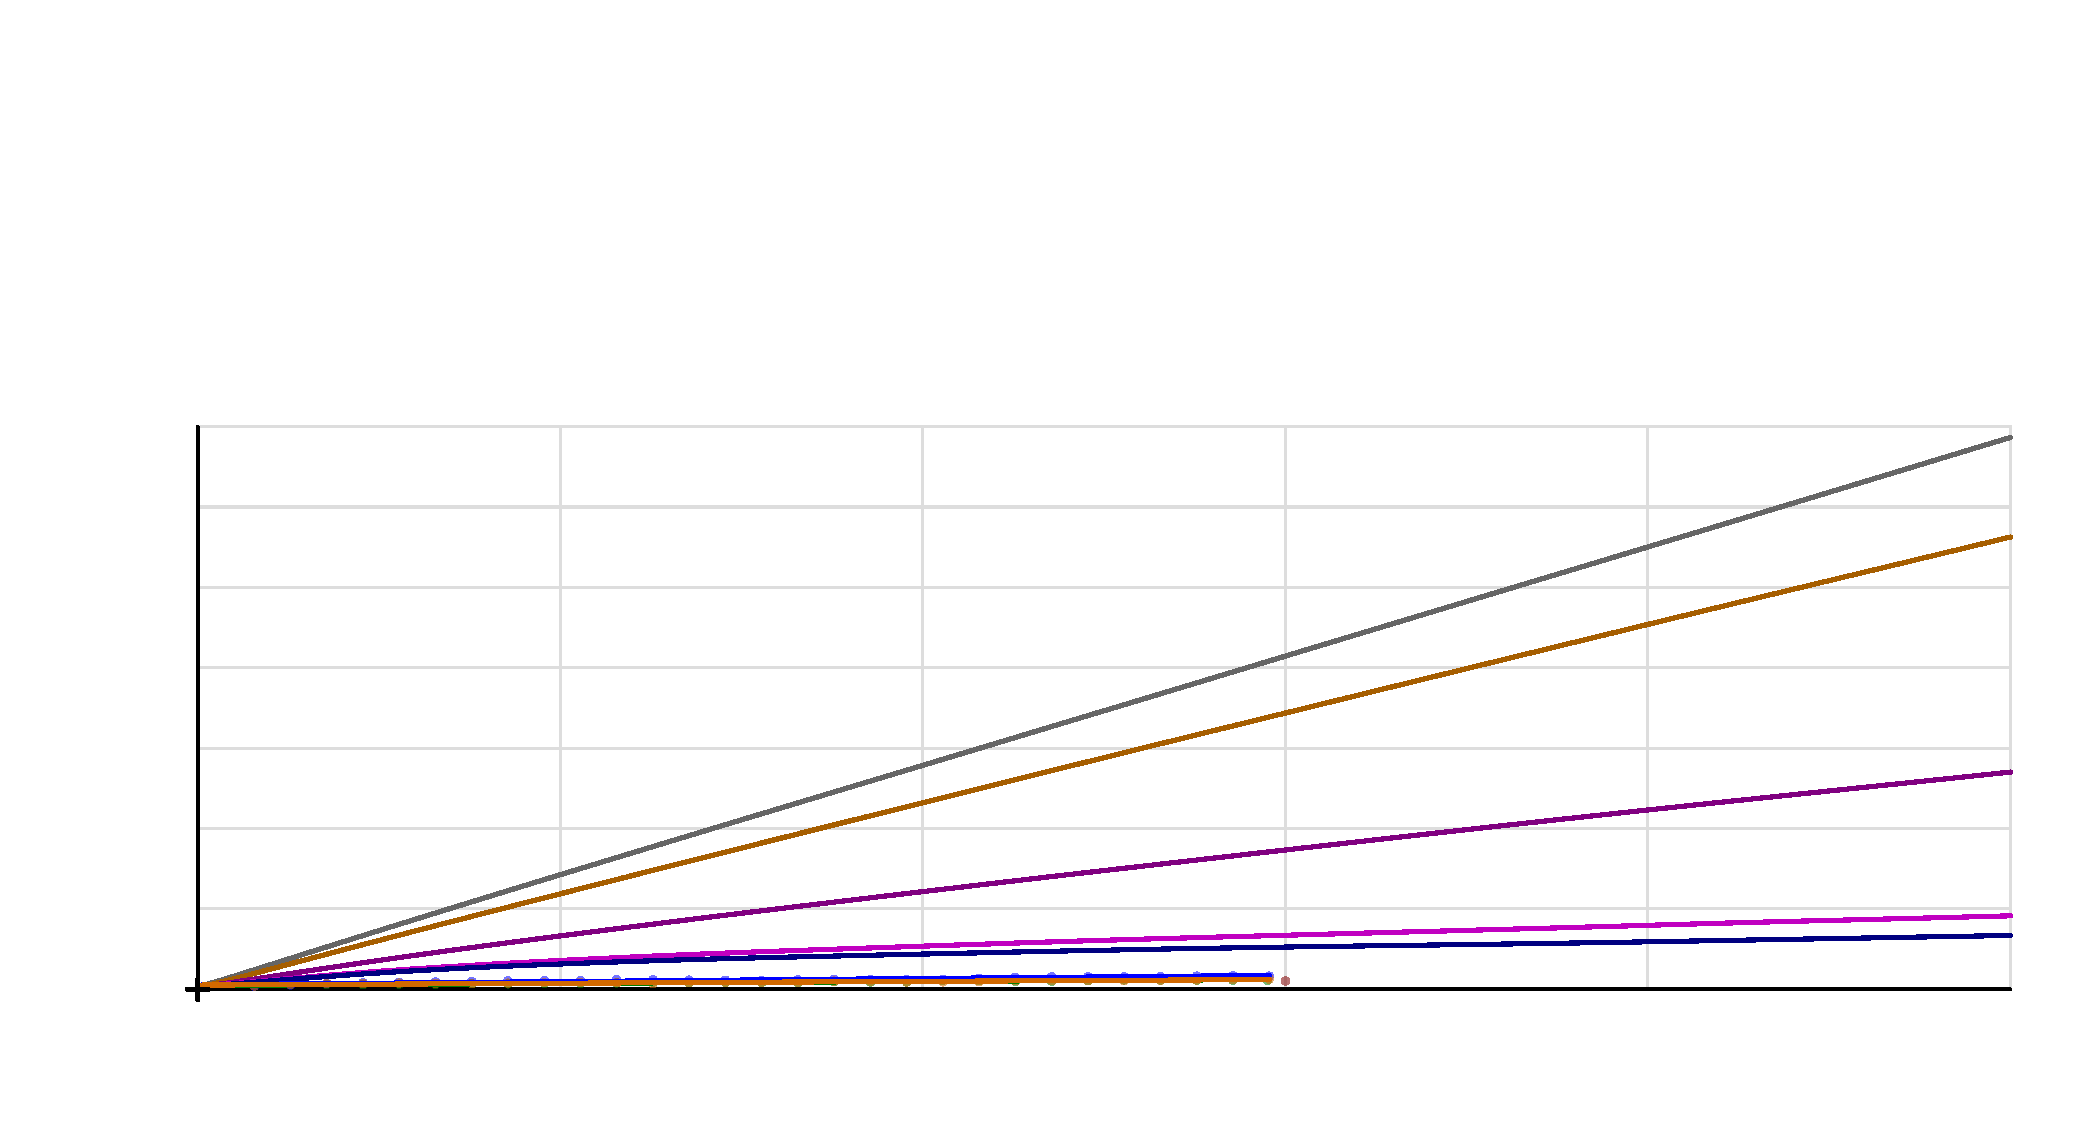
\includegraphics[width=1000.0bp,height=545.0bp]{figures/historical_comparison_zh.pdf}}
\put(95.0,522.0){\makebox(0,0)[lb]{\color{black}\sffamily\fontsize{16}{16}\selectfont HRMS(dAge){\cjkfont ：}\allowbreak{}{\cjkfont 历}\allowbreak{}{\cjkfont 史}\allowbreak{}{\cjkfont 研}\allowbreak{}{\cjkfont 究}\allowbreak{}{\cjkfont 与}\allowbreak{}{\cjkfont 新}\allowbreak{}{\cjkfont 结}\allowbreak{}{\cjkfont 果}\allowbreak{}}}
\put(95.0,50.0){\makebox(0,0)[cb]{\color{black}\sffamily\fontsize{12}{12}\selectfont 0}}
\put(269.0,50.0){\makebox(0,0)[cb]{\color{black}\sffamily\fontsize{12}{12}\selectfont 100}}
\put(443.0,50.0){\makebox(0,0)[cb]{\color{black}\sffamily\fontsize{12}{12}\selectfont 200}}
\put(617.0,50.0){\makebox(0,0)[cb]{\color{black}\sffamily\fontsize{12}{12}\selectfont 300}}
\put(791.0,50.0){\makebox(0,0)[cb]{\color{black}\sffamily\fontsize{12}{12}\selectfont 400}}
\put(965.0,50.0){\makebox(0,0)[cb]{\color{black}\sffamily\fontsize{12}{12}\selectfont 500}}
\put(87.0,66.0){\makebox(0,0)[rb]{\color{black}\sffamily\fontsize{12}{12}\selectfont 0}}
\put(87.0,104.57142857142856){\makebox(0,0)[rb]{\color{black}\sffamily\fontsize{12}{12}\selectfont 200}}
\put(87.0,143.1428571428571){\makebox(0,0)[rb]{\color{black}\sffamily\fontsize{12}{12}\selectfont 400}}
\put(87.0,181.71428571428572){\makebox(0,0)[rb]{\color{black}\sffamily\fontsize{12}{12}\selectfont 600}}
\put(87.0,220.28571428571428){\makebox(0,0)[rb]{\color{black}\sffamily\fontsize{12}{12}\selectfont 800}}
\put(87.0,258.8571428571429){\makebox(0,0)[rb]{\color{black}\sffamily\fontsize{12}{12}\selectfont 1000}}
\put(87.0,297.42857142857144){\makebox(0,0)[rb]{\color{black}\sffamily\fontsize{12}{12}\selectfont 1200}}
\put(87.0,336.0){\makebox(0,0)[rb]{\color{black}\sffamily\fontsize{12}{12}\selectfont 1400}}
\put(95.0,500.0){\makebox(0,0)[lb]{\color{red}\sffamily\fontsize{12}{12}\selectfont P23M\_0}}
\put(530.0,500.0){\makebox(0,0)[lb]{\color{green}\sffamily\fontsize{12}{12}\selectfont P23M\_1}}
\put(95.0,478.0){\makebox(0,0)[lb]{\color{blue}\sffamily\fontsize{12}{12}\selectfont UM980}}
\put(530.0,478.0){\makebox(0,0)[lb]{\color[HTML]{d26900}\sffamily\fontsize{12}{12}\selectfont LG290P}}
\put(95.0,456.0){\makebox(0,0)[lb]{\color[HTML]{800000}\sffamily\fontsize{12}{12}\selectfont {\cjkfont 历}\allowbreak{}{\cjkfont 史}\allowbreak{}{\cjkfont ：}\allowbreak{}{\cjkfont 精}\allowbreak{}{\cjkfont 密}\allowbreak{}{\cjkfont 钟}\allowbreak{}{\cjkfont 差}\allowbreak{}{\cjkfont （}\allowbreak{}{\cjkfont 单}\allowbreak{}{\cjkfont 点}\allowbreak{}{\cjkfont ）}\allowbreak{}}}
\put(95.0,434.0){\makebox(0,0)[lb]{\color[HTML]{666666}\sffamily\fontsize{12}{12}\selectfont {\cjkfont 历}\allowbreak{}{\cjkfont 史}\allowbreak{}{\cjkfont ：}\allowbreak{}{\cjkfont 无}\allowbreak{}{\cjkfont 卫}\allowbreak{}{\cjkfont 星}\allowbreak{}{\cjkfont 钟}\allowbreak{}{\cjkfont 差}\allowbreak{}}}
\put(530.0,434.0){\makebox(0,0)[lb]{\color[HTML]{a65e00}\sffamily\fontsize{12}{12}\selectfont {\cjkfont 历}\allowbreak{}{\cjkfont 史}\allowbreak{}{\cjkfont ：}\allowbreak{}{\cjkfont 卫}\allowbreak{}{\cjkfont 星}\allowbreak{}{\cjkfont 钟}\allowbreak{}{\cjkfont 差}\allowbreak{}}}
\put(95.0,412.0){\makebox(0,0)[lb]{\color[HTML]{800080}\sffamily\fontsize{12}{12}\selectfont {\cjkfont 历}\allowbreak{}{\cjkfont 史}\allowbreak{}{\cjkfont ：}\allowbreak{}{\cjkfont 卫}\allowbreak{}{\cjkfont 星}\allowbreak{}{\cjkfont 钟}\allowbreak{}{\cjkfont 差}\allowbreak{}{\cjkfont 及}\allowbreak{}{\cjkfont 相}\allowbreak{}{\cjkfont 对}\allowbreak{}{\cjkfont 论}\allowbreak{}{\cjkfont 修}\allowbreak{}{\cjkfont 正}\allowbreak{}}}
\put(530.0,412.0){\makebox(0,0)[lb]{\color[HTML]{c000c0}\sffamily\fontsize{12}{12}\selectfont {\cjkfont 历}\allowbreak{}{\cjkfont 史}\allowbreak{}{\cjkfont ：}\allowbreak{}{\cjkfont 加}\allowbreak{}{\cjkfont 超}\allowbreak{}{\cjkfont 快}\allowbreak{}{\cjkfont 速}\allowbreak{}{\cjkfont 产}\allowbreak{}{\cjkfont 品}\allowbreak{}}}
\put(95.0,390.0){\makebox(0,0)[lb]{\color[HTML]{000080}\sffamily\fontsize{12}{12}\selectfont {\cjkfont 历}\allowbreak{}{\cjkfont 史}\allowbreak{}{\cjkfont ：}\allowbreak{}{\cjkfont 加}\allowbreak{}{\cjkfont 精}\allowbreak{}{\cjkfont 密}\allowbreak{}{\cjkfont 轨}\allowbreak{}{\cjkfont 道}\allowbreak{}}}
\put(530.0,390.0){\makebox(0,0)[lb]{\color{green}\sffamily\fontsize{12}{12}\selectfont P23M\_1: +0.0492 mm/\allowbreak{}s}}
\put(95.0,368.0){\makebox(0,0)[lb]{\color{blue}\sffamily\fontsize{12}{12}\selectfont UM980: +0.0781 mm/\allowbreak{}s}}
\put(530.0,368.0){\makebox(0,0)[lb]{\color[HTML]{d26900}\sffamily\fontsize{12}{12}\selectfont LG290P: +0.0466 mm/\allowbreak{}s}}
\put(103.0,78.0){\makebox(0,0)[lb]{\color{black}\sffamily\fontsize{12}{12}\selectfont (0,0)}}
\put(530.0,12.0){\makebox(0,0)[cb]{\color{black}\sffamily\fontsize{12}{12}\selectfont {\cjkfont 改}\allowbreak{}{\cjkfont 正}\allowbreak{}{\cjkfont 数}\allowbreak{}{\cjkfont 据}\allowbreak{}{\cjkfont 龄}\allowbreak{}{\cjkfont 期}\allowbreak{} dAge [s]}}
\put(19.0,205.0){\rotatebox{90}{\makebox(0,0)[b]{\color{black}\sffamily\fontsize{12}{12}\selectfont {\cjkfont 水}\allowbreak{}{\cjkfont 平}\allowbreak{}{\cjkfont 均}\allowbreak{}{\cjkfont 方}\allowbreak{}{\cjkfont 根}\allowbreak{}{\cjkfont 误}\allowbreak{}{\cjkfont 差}\allowbreak{} HRMS [mm]}}}
\end{picture}}
\end{figure}
\begin{figure}[p]\centering
\resizebox{0.98\linewidth}{!}{%
\setlength{\unitlength}{1bp}\begin{picture}(1000.0,523.0)
\put(0,0){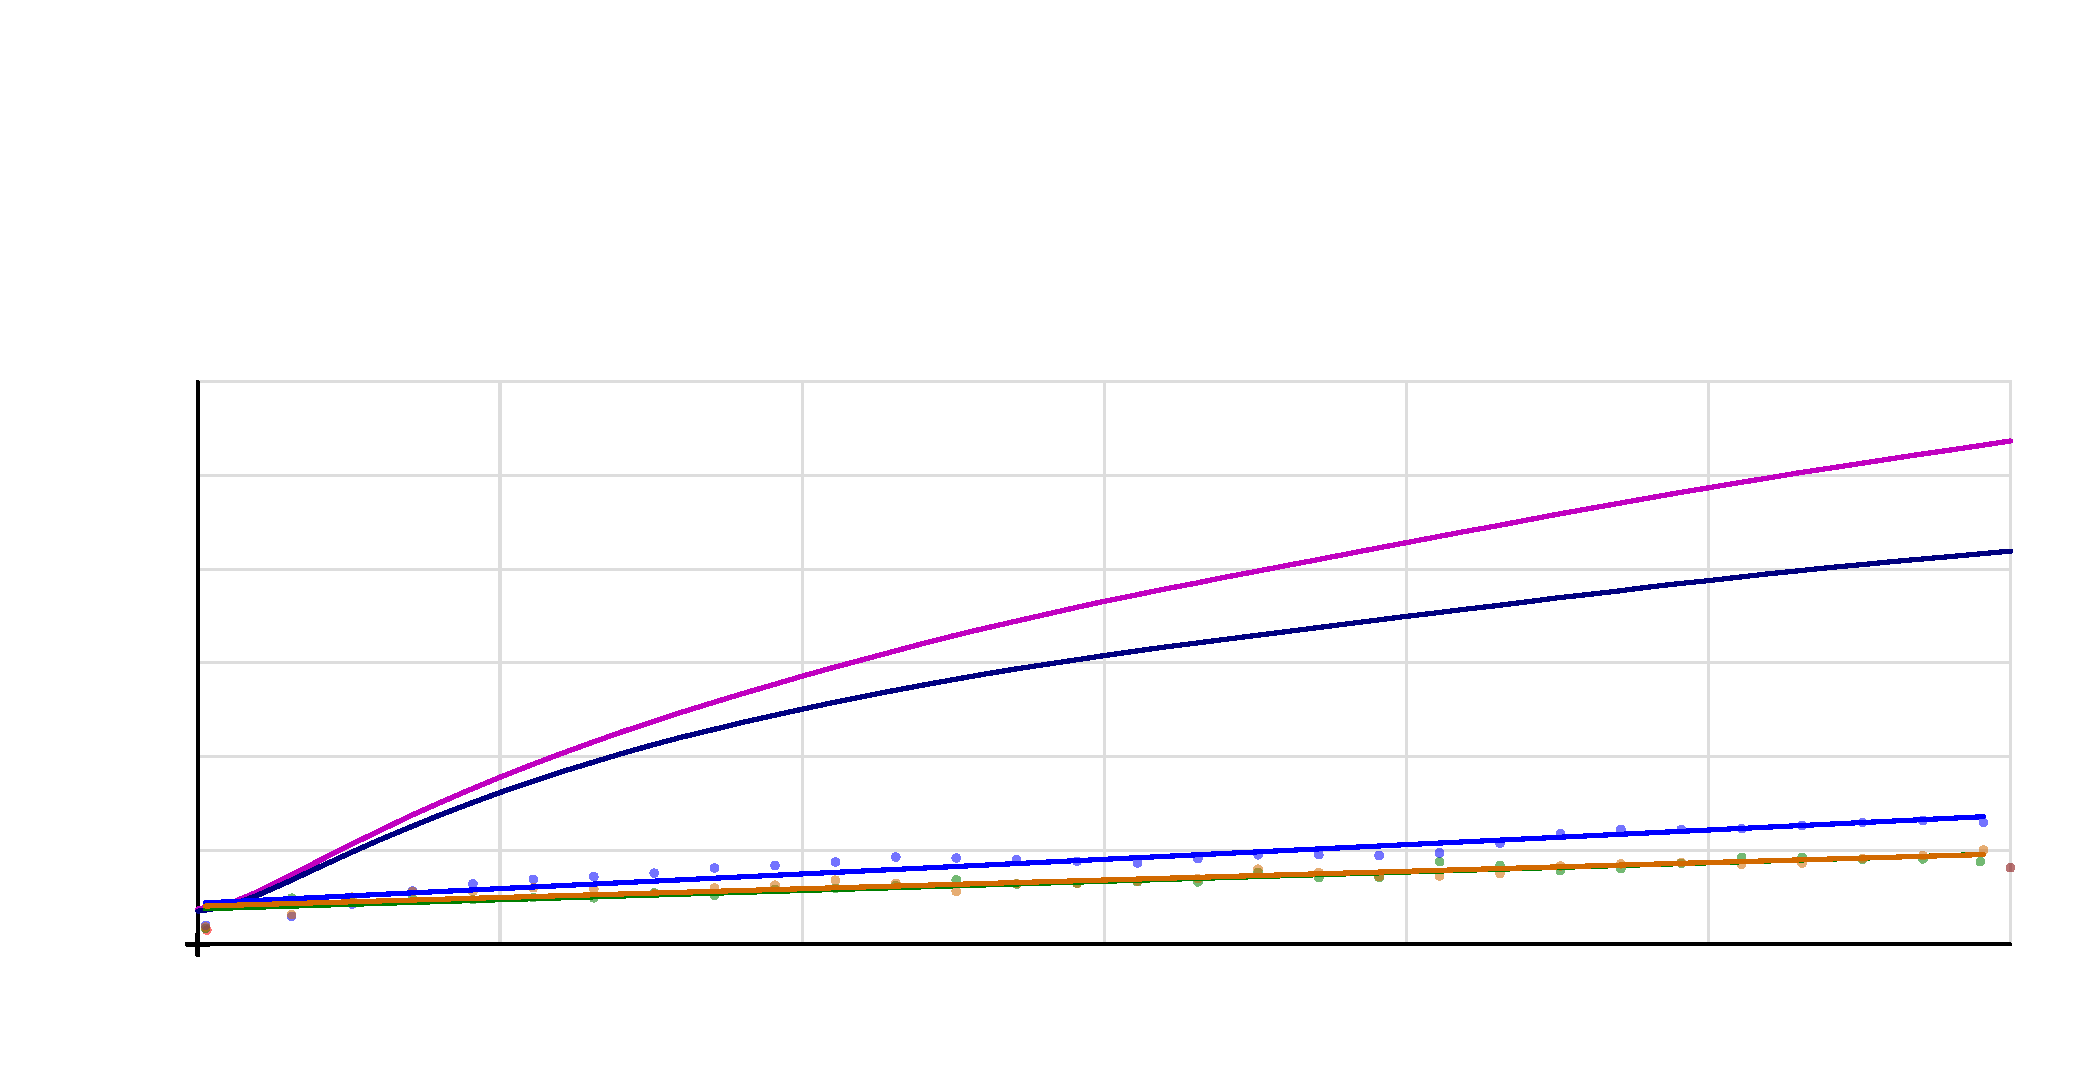
\includegraphics[width=1000.0bp,height=523.0bp]{figures/historical_comparison_detail_zh.pdf}}
\put(95.0,500.0){\makebox(0,0)[lb]{\color{black}\sffamily\fontsize{16}{16}\selectfont HRMS(dAge){\cjkfont ：}\allowbreak{}{\cjkfont 局}\allowbreak{}{\cjkfont 部}\allowbreak{}{\cjkfont 对}\allowbreak{}{\cjkfont 比}\allowbreak{}{\cjkfont （}\allowbreak{}0–300 {\cjkfont 秒}\allowbreak{}{\cjkfont ，}\allowbreak{}0–150 mm{\cjkfont ）}\allowbreak{}}}
\put(95.0,50.0){\makebox(0,0)[cb]{\color{black}\sffamily\fontsize{12}{12}\selectfont 0}}
\put(240.0,50.0){\makebox(0,0)[cb]{\color{black}\sffamily\fontsize{12}{12}\selectfont 50}}
\put(385.0,50.0){\makebox(0,0)[cb]{\color{black}\sffamily\fontsize{12}{12}\selectfont 100}}
\put(530.0,50.0){\makebox(0,0)[cb]{\color{black}\sffamily\fontsize{12}{12}\selectfont 150}}
\put(675.0,50.0){\makebox(0,0)[cb]{\color{black}\sffamily\fontsize{12}{12}\selectfont 200}}
\put(820.0,50.0){\makebox(0,0)[cb]{\color{black}\sffamily\fontsize{12}{12}\selectfont 250}}
\put(965.0,50.0){\makebox(0,0)[cb]{\color{black}\sffamily\fontsize{12}{12}\selectfont 300}}
\put(87.0,66.0){\makebox(0,0)[rb]{\color{black}\sffamily\fontsize{12}{12}\selectfont 0}}
\put(87.0,111.0){\makebox(0,0)[rb]{\color{black}\sffamily\fontsize{12}{12}\selectfont 25}}
\put(87.0,156.0){\makebox(0,0)[rb]{\color{black}\sffamily\fontsize{12}{12}\selectfont 50}}
\put(87.0,201.0){\makebox(0,0)[rb]{\color{black}\sffamily\fontsize{12}{12}\selectfont 75}}
\put(87.0,246.0){\makebox(0,0)[rb]{\color{black}\sffamily\fontsize{12}{12}\selectfont 100}}
\put(87.0,291.0){\makebox(0,0)[rb]{\color{black}\sffamily\fontsize{12}{12}\selectfont 125}}
\put(87.0,336.0){\makebox(0,0)[rb]{\color{black}\sffamily\fontsize{12}{12}\selectfont 150}}
\put(95.0,478.0){\makebox(0,0)[lb]{\color{red}\sffamily\fontsize{12}{12}\selectfont P23M\_0}}
\put(530.0,478.0){\makebox(0,0)[lb]{\color{green}\sffamily\fontsize{12}{12}\selectfont P23M\_1}}
\put(95.0,456.0){\makebox(0,0)[lb]{\color{blue}\sffamily\fontsize{12}{12}\selectfont UM980}}
\put(530.0,456.0){\makebox(0,0)[lb]{\color[HTML]{d26900}\sffamily\fontsize{12}{12}\selectfont LG290P}}
\put(95.0,434.0){\makebox(0,0)[lb]{\color[HTML]{800000}\sffamily\fontsize{12}{12}\selectfont {\cjkfont 历}\allowbreak{}{\cjkfont 史}\allowbreak{}{\cjkfont ：}\allowbreak{}{\cjkfont 精}\allowbreak{}{\cjkfont 密}\allowbreak{}{\cjkfont 钟}\allowbreak{}{\cjkfont 差}\allowbreak{}{\cjkfont （}\allowbreak{}{\cjkfont 单}\allowbreak{}{\cjkfont 点}\allowbreak{}{\cjkfont ）}\allowbreak{}}}
\put(95.0,412.0){\makebox(0,0)[lb]{\color[HTML]{c000c0}\sffamily\fontsize{12}{12}\selectfont {\cjkfont 历}\allowbreak{}{\cjkfont 史}\allowbreak{}{\cjkfont ：}\allowbreak{}{\cjkfont 加}\allowbreak{}{\cjkfont 超}\allowbreak{}{\cjkfont 快}\allowbreak{}{\cjkfont 速}\allowbreak{}{\cjkfont 产}\allowbreak{}{\cjkfont 品}\allowbreak{}}}
\put(530.0,412.0){\makebox(0,0)[lb]{\color[HTML]{000080}\sffamily\fontsize{12}{12}\selectfont {\cjkfont 历}\allowbreak{}{\cjkfont 史}\allowbreak{}{\cjkfont ：}\allowbreak{}{\cjkfont 加}\allowbreak{}{\cjkfont 精}\allowbreak{}{\cjkfont 密}\allowbreak{}{\cjkfont 轨}\allowbreak{}{\cjkfont 道}\allowbreak{}}}
\put(95.0,390.0){\makebox(0,0)[lb]{\color{green}\sffamily\fontsize{12}{12}\selectfont P23M\_1: +0.0492 mm/\allowbreak{}s}}
\put(530.0,390.0){\makebox(0,0)[lb]{\color{blue}\sffamily\fontsize{12}{12}\selectfont UM980: +0.0781 mm/\allowbreak{}s}}
\put(95.0,368.0){\makebox(0,0)[lb]{\color[HTML]{d26900}\sffamily\fontsize{12}{12}\selectfont LG290P: +0.0466 mm/\allowbreak{}s}}
\put(103.0,78.0){\makebox(0,0)[lb]{\color{black}\sffamily\fontsize{12}{12}\selectfont (0,0)}}
\put(530.0,12.0){\makebox(0,0)[cb]{\color{black}\sffamily\fontsize{12}{12}\selectfont {\cjkfont 改}\allowbreak{}{\cjkfont 正}\allowbreak{}{\cjkfont 数}\allowbreak{}{\cjkfont 据}\allowbreak{}{\cjkfont 龄}\allowbreak{}{\cjkfont 期}\allowbreak{} dAge [s]}}
\put(19.0,205.0){\rotatebox{90}{\makebox(0,0)[b]{\color{black}\sffamily\fontsize{12}{12}\selectfont {\cjkfont 水}\allowbreak{}{\cjkfont 平}\allowbreak{}{\cjkfont 均}\allowbreak{}{\cjkfont 方}\allowbreak{}{\cjkfont 根}\allowbreak{}{\cjkfont 误}\allowbreak{}{\cjkfont 差}\allowbreak{} HRMS [mm]}}}
\end{picture}}
\end{figure}\clearpage
\end{document}
